\documentclass[10pt]{report}% ===> this file was generated automatically by noweave --- better not edit it
\usepackage {noweb}
\usepackage {graphicx}
\graphicspath { {./images/} }

\usepackage[table,dvipsnames]{xcolor}
\definecolor {apple_white}{rgb}{0.9,0.9,0.9}
\def \bk0 {\cellcolor{black}}
\def \bl0 {\cellcolor{Cerulean}}
\def \bw0 {\cellcolor{apple_white}}
\def \bo0 {\cellcolor{orange}}

\usepackage {booktabs}
\usepackage {tikz}
\usetikzlibrary {positioning, shapes.geometric, svg.path}

\noweboptions {smallcode,longchunks}

% Generate assembly file with:
% notangle -Rpreamble main.nw > main.asm
%
% Generate tex file with:
% noweave -delay -index main.nw > main.tex
% pdflatex main.tex (run twice for two passes)
% Indents in code only appears in the PDF output
% under TeX Live 2019.
%
% See also: https://www.cs.tufts.edu/~nr/noweb/johnson-lj.pdf

\begin{document}
\pagestyle{noweb}

\nwfilename{main.nw}\nwbegindocs{1}\chapter{Lode Runner}

Lode Runner was a game originally written in 1982 by Douglas E. Smith (1960--2014) for
the Apple II series of computers, and published by Broderbund.

\begin{center}
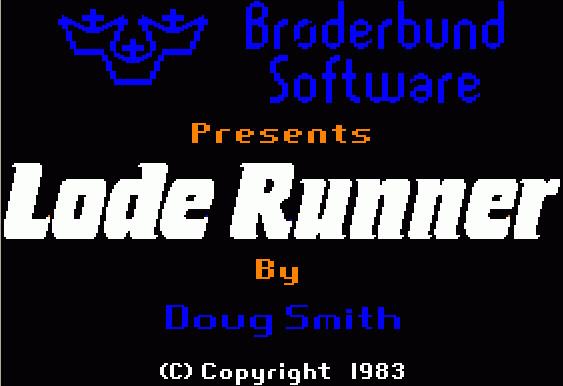
\includegraphics[width=\columnwidth]{title-screen}
\end{center}

You control the movement of your character, moving left and right along brick
and bedrock platforms, climbing ladders,
and "monkey-traversing" ropes strung across gaps. The object is to collect all the
gold boxes while avoiding being touched by the guards. You can dig holes in
brick parts of the floor which can allow you to reach otherwise unreachable caverns,
and the holes can also trap the guards for a short while. Holes fill themselves in
after a short time period, and if you're in a hole when that happens, you lose
a life. However, if a guard is in the hole and the hole fills, the guard disappears and
reappears somewhere along the top of the screen.

You get points for collecting boxes and forcing guards to respawn. Once you collect
all the boxes, a ladder will appear leading out of the top of the screen. This
gets you to the next level, and play continues.

\begin{center}
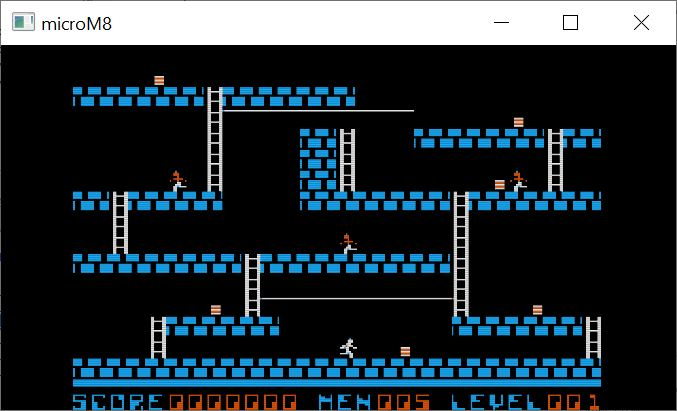
\includegraphics[width=\columnwidth]{screen}
\end{center}

Lode Runner included 150 levels and also a level editor.

\chapter{Apple II Graphics}
Hi-res graphics on the Apple II is odd. Graphics are memory-mapped, not exactly
consecutively, and bits don't always correspond to pixels. Color especially is
odd, compared to today's luxurious 32-bit per pixel RGBA.

The Apple II has two hi-res graphics pages, and maps the area from {\Tt{}{\$}2000-{\$}3FFF\nwendquote} to
high-res graphics page 1 (HGR1), and {\Tt{}{\$}4000-{\$}5FFF\nwendquote} to page 2 (HGR2).

We have routines to clear these screens.

\nwenddocs{}\nwbegincode{2}\sublabel{NW1Xx3lK-10jlgu-1}\nwmargintag{{\nwtagstyle{}\subpageref{NW1Xx3lK-10jlgu-1}}}\moddef{defines~{\nwtagstyle{}\subpageref{NW1Xx3lK-10jlgu-1}}}\endmoddef\nwstartdeflinemarkup\nwusesondefline{\\{NW1Xx3lK-1p0Y9w-1}}\nwprevnextdefs{\relax}{NW1Xx3lK-10jlgu-2}\nwenddeflinemarkup
    ORG     $0A
\nwlinkedidentc{TMP_PTR}{NW1Xx3lK-10jlgu-1}         DS.W    1
\nwindexdefn{\nwixident{TMP{\_}PTR}}{TMP:unPTR}{NW1Xx3lK-10jlgu-1}\eatline
\nwalsodefined{\\{NW1Xx3lK-10jlgu-2}\\{NW1Xx3lK-10jlgu-3}\\{NW1Xx3lK-10jlgu-4}\\{NW1Xx3lK-10jlgu-5}\\{NW1Xx3lK-10jlgu-6}\\{NW1Xx3lK-10jlgu-7}\\{NW1Xx3lK-10jlgu-8}\\{NW1Xx3lK-10jlgu-9}\\{NW1Xx3lK-10jlgu-A}\\{NW1Xx3lK-10jlgu-B}\\{NW1Xx3lK-10jlgu-C}\\{NW1Xx3lK-10jlgu-D}\\{NW1Xx3lK-10jlgu-E}\\{NW1Xx3lK-10jlgu-F}\\{NW1Xx3lK-10jlgu-G}\\{NW1Xx3lK-10jlgu-H}\\{NW1Xx3lK-10jlgu-I}\\{NW1Xx3lK-10jlgu-J}\\{NW1Xx3lK-10jlgu-K}\\{NW1Xx3lK-10jlgu-L}\\{NW1Xx3lK-10jlgu-M}\\{NW1Xx3lK-10jlgu-N}\\{NW1Xx3lK-10jlgu-O}\\{NW1Xx3lK-10jlgu-P}\\{NW1Xx3lK-10jlgu-Q}\\{NW1Xx3lK-10jlgu-R}\\{NW1Xx3lK-10jlgu-S}}\nwused{\\{NW1Xx3lK-1p0Y9w-1}}\nwidentdefs{\\{{\nwixident{TMP{\_}PTR}}{TMP:unPTR}}}\nwendcode{}\nwbegindocs{3}\nwdocspar
\nwenddocs{}\nwbegincode{4}\sublabel{NW1Xx3lK-8jv1b-1}\nwmargintag{{\nwtagstyle{}\subpageref{NW1Xx3lK-8jv1b-1}}}\moddef{routines~{\nwtagstyle{}\subpageref{NW1Xx3lK-8jv1b-1}}}\endmoddef\nwstartdeflinemarkup\nwusesondefline{\\{NW1Xx3lK-1p0Y9w-1}}\nwprevnextdefs{\relax}{NW1Xx3lK-8jv1b-2}\nwenddeflinemarkup
    ORG     $7A51
\nwlinkedidentc{CLEAR_HGR1}{NW1Xx3lK-8jv1b-1}:
    SUBROUTINE

    LDA     #$20                ; Start at $2000
    LDX     #$40                ; End at $4000 (but not including)
    BNE     CLEAR_PAGE          ; Unconditional jump

\nwlinkedidentc{CLEAR_HGR2}{NW1Xx3lK-8jv1b-1}:
    SUBROUTINE

    LDA     #$40                ; Start at $4000
    LDX     #$60                ; End at $6000 (but not including)
    ; fallthrough

CLEAR_PAGE:
    STA     \nwlinkedidentc{TMP_PTR}{NW1Xx3lK-10jlgu-1}+1           ; Start with the page in A.
    LDA     #$00
    STA     \nwlinkedidentc{TMP_PTR}{NW1Xx3lK-10jlgu-1}
    TAY
    LDA     #$80                ; fill byte = 0x80

.loop:
    STA     (\nwlinkedidentc{TMP_PTR}{NW1Xx3lK-10jlgu-1}),Y
    INY
    BNE     .loop
    INC     \nwlinkedidentc{TMP_PTR}{NW1Xx3lK-10jlgu-1}+1
    CPX     \nwlinkedidentc{TMP_PTR}{NW1Xx3lK-10jlgu-1}+1
    BNE     .loop               ; while \nwlinkedidentc{TMP_PTR}{NW1Xx3lK-10jlgu-1} != X * 0x100
    RTS
\nwindexdefn{\nwixident{CLEAR{\_}HGR1}}{CLEAR:unHGR1}{NW1Xx3lK-8jv1b-1}\nwindexdefn{\nwixident{CLEAR{\_}HGR2}}{CLEAR:unHGR2}{NW1Xx3lK-8jv1b-1}\eatline
\nwalsodefined{\\{NW1Xx3lK-8jv1b-2}\\{NW1Xx3lK-8jv1b-3}\\{NW1Xx3lK-8jv1b-4}\\{NW1Xx3lK-8jv1b-5}\\{NW1Xx3lK-8jv1b-6}\\{NW1Xx3lK-8jv1b-7}\\{NW1Xx3lK-8jv1b-8}\\{NW1Xx3lK-8jv1b-9}\\{NW1Xx3lK-8jv1b-A}\\{NW1Xx3lK-8jv1b-B}\\{NW1Xx3lK-8jv1b-C}\\{NW1Xx3lK-8jv1b-D}\\{NW1Xx3lK-8jv1b-E}\\{NW1Xx3lK-8jv1b-F}\\{NW1Xx3lK-8jv1b-G}\\{NW1Xx3lK-8jv1b-H}\\{NW1Xx3lK-8jv1b-I}\\{NW1Xx3lK-8jv1b-J}\\{NW1Xx3lK-8jv1b-K}}\nwused{\\{NW1Xx3lK-1p0Y9w-1}}\nwidentdefs{\\{{\nwixident{CLEAR{\_}HGR1}}{CLEAR:unHGR1}}\\{{\nwixident{CLEAR{\_}HGR2}}{CLEAR:unHGR2}}}\nwidentuses{\\{{\nwixident{TMP{\_}PTR}}{TMP:unPTR}}}\nwindexuse{\nwixident{TMP{\_}PTR}}{TMP:unPTR}{NW1Xx3lK-8jv1b-1}\nwendcode{}\nwbegindocs{5}\nwdocspar
\section{Pixels and their color}
First we'll talk about pixels. Nominally, the resolution of the hi-res graphics screen
is 280 pixels wide by 192 pixels tall. In the memory map, each row is represented
by 40 bytes. The high bit of each byte is not used for pixel data, but is used to
control color.

Here are some rules for how these bytes are turned into pixels:
\begin{itemize}
  \item Pixels are drawn to the screen from byte data least significant bit first.
        This means that for the first byte bit 0 is column 0, bit 1 is column 1,
        and so on.
  \item A pattern of {\Tt{}11\nwendquote} results in two white pixels at the {\Tt{}1\nwendquote} positions.
  \item A pattern of {\Tt{}010\nwendquote} results at least in a colored pixel at the {\Tt{}1\nwendquote} position.
  \item A pattern of {\Tt{}101\nwendquote} results at least in a colored pixel at the {\Tt{}0\nwendquote} position.
  \item So, a pattern of {\Tt{}01010\nwendquote} results in at least three consecutive colored
        pixels starting from the first {\Tt{}1\nwendquote} to the last {\Tt{}1\nwendquote}. The last {\Tt{}0\nwendquote} bit
        would also be colored if followed by a {\Tt{}1\nwendquote}.
  \item Likewise, a pattern of {\Tt{}11011\nwendquote} results in two white pixels, a colored pixel,
        and then two more white pixels.
  \item The color of a {\Tt{}010\nwendquote} pixel depends on the column that the {\Tt{}1\nwendquote} falls on, and
        also whether the high bit of its byte was set or not. 
  \item The color of a {\Tt{}11011\nwendquote} pixel depends on the column that the {\Tt{}0\nwendquote} falls on, and
        also whether the high bit of its byte was set or not.

        \begin{center}
        \begin{tabular}{@{}rcc@{}} \toprule
        & Odd & Even \\ \cmidrule(r){2-3}
        High bit clear & Green & Violet \\
        High bit set & Orange & Blue \\ \bottomrule
        \end{tabular}
        \end{center}

        The implication is that you can only select one pair of colors per byte.
\end{itemize}

An example would probably be good here. We will take one of the sprites from the game.

\begin{center}
\begin{tabular}{@{}rcc@{}} \toprule
Bytes & Bits & Pixel Data \\ \cmidrule{1-3}
{\Tt{}00\ 00\nwendquote} & {\Tt{}0000000\ 0000000\nwendquote} & {\Tt{}00000000000000\nwendquote} \\
{\Tt{}00\ 00\nwendquote} & {\Tt{}0000000\ 0000000\nwendquote} & {\Tt{}00000000000000\nwendquote} \\
{\Tt{}00\ 00\nwendquote} & {\Tt{}0000000\ 0000000\nwendquote} & {\Tt{}00000000000000\nwendquote} \\
{\Tt{}55\ 00\nwendquote} & {\Tt{}1010101\ 0000000\nwendquote} & {\Tt{}10101010000000\nwendquote} \\
{\Tt{}41\ 00\nwendquote} & {\Tt{}1000001\ 0000000\nwendquote} & {\Tt{}10000010000000\nwendquote} \\
{\Tt{}01\ 00\nwendquote} & {\Tt{}0000001\ 0000000\nwendquote} & {\Tt{}10000000000000\nwendquote} \\
{\Tt{}55\ 00\nwendquote} & {\Tt{}1010101\ 0000000\nwendquote} & {\Tt{}10101010000000\nwendquote} \\
{\Tt{}50\ 00\nwendquote} & {\Tt{}1010000\ 0000000\nwendquote} & {\Tt{}00001010000000\nwendquote} \\
{\Tt{}50\ 00\nwendquote} & {\Tt{}1010000\ 0000000\nwendquote} & {\Tt{}00001010000000\nwendquote} \\
{\Tt{}51\ 00\nwendquote} & {\Tt{}1010001\ 0000000\nwendquote} & {\Tt{}10001010000000\nwendquote} \\
{\Tt{}55\ 00\nwendquote} & {\Tt{}1010101\ 0000000\nwendquote} & {\Tt{}10101010000000\nwendquote} \\ \bottomrule
\end{tabular}
\end{center}

The game automatically sets the high bit of each byte, so we know we're going to see
orange and blue. Assuming that the following bits are all zero, and we place the
sprite starting at column 0, we should see this:

\begin{center}
\begin{tabular}{@{}rcccccccccccccc@{}}
 0 & \bk0 & \bk0 & \bk0 & \bk0 & \bk0 & \bk0 & \bk0 & \bk0 & \bk0 & \bk0 & \bk0 & \bk0 & \bk0 & \bk0 \\
 1 & \bk0 & \bk0 & \bk0 & \bk0 & \bk0 & \bk0 & \bk0 & \bk0 & \bk0 & \bk0 & \bk0 & \bk0 & \bk0 & \bk0 \\
 2 & \bk0 & \bk0 & \bk0 & \bk0 & \bk0 & \bk0 & \bk0 & \bk0 & \bk0 & \bk0 & \bk0 & \bk0 & \bk0 & \bk0 \\
 3 & \bl0 & \bl0 & \bl0 & \bl0 & \bl0 & \bl0 & \bl0 & \bk0 & \bk0 & \bk0 & \bk0 & \bk0 & \bk0 & \bk0 \\
 4 & \bl0 & \bk0 & \bk0 & \bk0 & \bk0 & \bk0 & \bl0 & \bk0 & \bk0 & \bk0 & \bk0 & \bk0 & \bk0 & \bk0 \\
 5 & \bl0 & \bk0 & \bk0 & \bk0 & \bk0 & \bk0 & \bk0 & \bk0 & \bk0 & \bk0 & \bk0 & \bk0 & \bk0 & \bk0 \\
 6 & \bl0 & \bl0 & \bl0 & \bl0 & \bl0 & \bl0 & \bl0 & \bk0 & \bk0 & \bk0 & \bk0 & \bk0 & \bk0 & \bk0 \\
 7 & \bk0 & \bk0 & \bk0 & \bk0 & \bl0 & \bl0 & \bl0 & \bk0 & \bk0 & \bk0 & \bk0 & \bk0 & \bk0 & \bk0 \\
 8 & \bk0 & \bk0 & \bk0 & \bk0 & \bl0 & \bl0 & \bl0 & \bk0 & \bk0 & \bk0 & \bk0 & \bk0 & \bk0 & \bk0 \\
 9 & \bl0 & \bk0 & \bk0 & \bk0 & \bl0 & \bl0 & \bl0 & \bk0 & \bk0 & \bk0 & \bk0 & \bk0 & \bk0 & \bk0 \\
10 & \bl0 & \bl0 & \bl0 & \bl0 & \bl0 & \bl0 & \bl0 & \bk0 & \bk0 & \bk0 & \bk0 & \bk0 & \bk0 & \bk0 \\
\end{tabular}
\end{center}

Here is a more complex sprite:

\begin{center}
\begin{tabular}{@{}rcc@{}} \toprule
Bytes & Bits & Pixel Data \\ \cmidrule{1-3}
{\Tt{}40\ 00\nwendquote} & {\Tt{}1000000\ 0000000\nwendquote} & {\Tt{}00000010000000\nwendquote} \\
{\Tt{}60\ 01\nwendquote} & {\Tt{}1100000\ 0000001\nwendquote} & {\Tt{}00000111000000\nwendquote} \\
{\Tt{}60\ 01\nwendquote} & {\Tt{}1100000\ 0000001\nwendquote} & {\Tt{}00000111000000\nwendquote} \\
{\Tt{}70\ 00\nwendquote} & {\Tt{}1110000\ 0000000\nwendquote} & {\Tt{}00001110000000\nwendquote} \\
{\Tt{}6C\ 01\nwendquote} & {\Tt{}1101100\ 0000001\nwendquote} & {\Tt{}00110111000000\nwendquote} \\
{\Tt{}36\ 06\nwendquote} & {\Tt{}0110110\ 0000110\nwendquote} & {\Tt{}01101100110000\nwendquote} \\
{\Tt{}30\ 00\nwendquote} & {\Tt{}0110000\ 0000000\nwendquote} & {\Tt{}00001100000000\nwendquote} \\
{\Tt{}70\ 00\nwendquote} & {\Tt{}1110000\ 0000000\nwendquote} & {\Tt{}00001110000000\nwendquote} \\
{\Tt{}5E\ 01\nwendquote} & {\Tt{}1011110\ 0000001\nwendquote} & {\Tt{}01111011000000\nwendquote} \\
{\Tt{}40\ 01\nwendquote} & {\Tt{}1000000\ 0000001\nwendquote} & {\Tt{}00000011000000\nwendquote} \\
{\Tt{}40\ 01\nwendquote} & {\Tt{}1000000\ 0000001\nwendquote} & {\Tt{}00000011000000\nwendquote} \\ \bottomrule
\end{tabular}
\end{center}

\begin{center}
\begin{tabular}{@{}rcccccccccccccc@{}}
0 & \bk0 & \bk0 & \bk0 & \bk0 & \bk0 & \bk0 & \bl0 & \bk0 & \bk0 & \bk0 & \bk0 & \bk0 & \bk0 & \bk0 \\
1 & \bk0 & \bk0 & \bk0 & \bk0 & \bk0 & \bw0 & \bw0 & \bw0 & \bk0 & \bk0 & \bk0 & \bk0 & \bk0 & \bk0 \\
2 & \bk0 & \bk0 & \bk0 & \bk0 & \bk0 & \bw0 & \bw0 & \bw0 & \bk0 & \bk0 & \bk0 & \bk0 & \bk0 & \bk0 \\
3 & \bk0 & \bk0 & \bk0 & \bk0 & \bw0 & \bw0 & \bw0 & \bk0 & \bk0 & \bk0 & \bk0 & \bk0 & \bk0 & \bk0 \\
4 & \bk0 & \bk0 & \bw0 & \bw0 & \bo0 & \bw0 & \bw0 & \bw0 & \bk0 & \bk0 & \bk0 & \bk0 & \bk0 & \bk0 \\
5 & \bk0 & \bw0 & \bw0 & \bl0 & \bw0 & \bw0 & \bk0 & \bk0 & \bw0 & \bw0 & \bk0 & \bk0 & \bk0 & \bk0 \\
6 & \bk0 & \bk0 & \bk0 & \bk0 & \bw0 & \bw0 & \bk0 & \bk0 & \bk0 & \bk0 & \bk0 & \bk0 & \bk0 & \bk0 \\
7 & \bk0 & \bk0 & \bk0 & \bk0 & \bw0 & \bw0 & \bw0 & \bk0 & \bk0 & \bk0 & \bk0 & \bk0 & \bk0 & \bk0 \\
8 & \bk0 & \bw0 & \bw0 & \bw0 & \bw0 & \bl0 & \bw0 & \bw0 & \bk0 & \bk0 & \bk0 & \bk0 & \bk0 & \bk0 \\
9 & \bk0 & \bk0 & \bk0 & \bk0 & \bk0 & \bk0 & \bw0 & \bw0 & \bk0 & \bk0 & \bk0 & \bk0 & \bk0 & \bk0 \\
10 & \bk0 & \bk0 & \bk0 & \bk0 & \bk0 & \bk0 & \bw0 & \bw0 & \bk0 & \bk0 & \bk0 & \bk0 & \bk0 & \bk0 \\
\end{tabular}
\end{center}

Take note of the orange and blue pixels. All the patterns noted in the rules above are used.

\section{The sprites}
Lode Runner defines 104 sprites, each being 11 rows, with two bytes per row. The first bytes of
all 104 sprites are in the table first, then the second bytes, then the third bytes, and so on.
Later we will see that only the leftmost 10 pixels out of the 14-pixel description is used.

\nwenddocs{}\nwbegincode{6}\sublabel{NW1Xx3lK-1W8AJS-1}\nwmargintag{{\nwtagstyle{}\subpageref{NW1Xx3lK-1W8AJS-1}}}\moddef{tables~{\nwtagstyle{}\subpageref{NW1Xx3lK-1W8AJS-1}}}\endmoddef\nwstartdeflinemarkup\nwusesondefline{\\{NW1Xx3lK-1p0Y9w-1}}\nwprevnextdefs{\relax}{NW1Xx3lK-1W8AJS-2}\nwenddeflinemarkup
    ORG     $AD00
\nwlinkedidentc{SPRITE_DATA}{NW1Xx3lK-1W8AJS-1}:
    INCLUDE "sprite_data.asm"
\nwindexdefn{\nwixident{SPRITE{\_}DATA}}{SPRITE:unDATA}{NW1Xx3lK-1W8AJS-1}\eatline
\nwalsodefined{\\{NW1Xx3lK-1W8AJS-2}\\{NW1Xx3lK-1W8AJS-3}\\{NW1Xx3lK-1W8AJS-4}\\{NW1Xx3lK-1W8AJS-5}\\{NW1Xx3lK-1W8AJS-6}\\{NW1Xx3lK-1W8AJS-7}\\{NW1Xx3lK-1W8AJS-8}\\{NW1Xx3lK-1W8AJS-9}\\{NW1Xx3lK-1W8AJS-A}\\{NW1Xx3lK-1W8AJS-B}\\{NW1Xx3lK-1W8AJS-C}\\{NW1Xx3lK-1W8AJS-D}\\{NW1Xx3lK-1W8AJS-E}\\{NW1Xx3lK-1W8AJS-F}\\{NW1Xx3lK-1W8AJS-G}\\{NW1Xx3lK-1W8AJS-H}}\nwused{\\{NW1Xx3lK-1p0Y9w-1}}\nwidentdefs{\\{{\nwixident{SPRITE{\_}DATA}}{SPRITE:unDATA}}}\nwendcode{}\nwbegindocs{7}\nwdocspar
\begin{center}
\scalebox{0.8}{
\begin{tabular}{@{}rcccccccccccccccccccccccccccccc@{}}
 & \multicolumn{14}{c}{Sprite 0} & & \multicolumn{14}{c}{Sprite 1} \\
0 & \bk0 & \bk0 & \bk0 & \bk0 & \bk0 & \bk0 & \bk0 & \bk0 & \bk0 & \bk0 & \bk0 & \bk0 & \bk0 & \bk0 & & \bl0 & \bl0 & \bl0 & \bl0 & \bl0 & \bk0 & \bk0 & \bk0 & \bl0 & \bk0 & \bk0 & \bk0 & \bk0 & \bk0 & \\
1 & \bk0 & \bk0 & \bk0 & \bk0 & \bk0 & \bk0 & \bk0 & \bk0 & \bk0 & \bk0 & \bk0 & \bk0 & \bk0 & \bk0 & & \bl0 & \bl0 & \bl0 & \bl0 & \bl0 & \bk0 & \bk0 & \bk0 & \bl0 & \bk0 & \bk0 & \bk0 & \bk0 & \bk0 & \\
2 & \bk0 & \bk0 & \bk0 & \bk0 & \bk0 & \bk0 & \bk0 & \bk0 & \bk0 & \bk0 & \bk0 & \bk0 & \bk0 & \bk0 & & \bl0 & \bl0 & \bl0 & \bl0 & \bl0 & \bk0 & \bk0 & \bk0 & \bl0 & \bk0 & \bk0 & \bk0 & \bk0 & \bk0 & \\
3 & \bk0 & \bk0 & \bk0 & \bk0 & \bk0 & \bk0 & \bk0 & \bk0 & \bk0 & \bk0 & \bk0 & \bk0 & \bk0 & \bk0 & & \bl0 & \bl0 & \bl0 & \bl0 & \bl0 & \bk0 & \bk0 & \bk0 & \bl0 & \bk0 & \bk0 & \bk0 & \bk0 & \bk0 & \\
4 & \bk0 & \bk0 & \bk0 & \bk0 & \bk0 & \bk0 & \bk0 & \bk0 & \bk0 & \bk0 & \bk0 & \bk0 & \bk0 & \bk0 & & \bk0 & \bk0 & \bk0 & \bk0 & \bk0 & \bk0 & \bk0 & \bk0 & \bk0 & \bk0 & \bk0 & \bk0 & \bk0 & \bk0 & \\
5 & \bk0 & \bk0 & \bk0 & \bk0 & \bk0 & \bk0 & \bk0 & \bk0 & \bk0 & \bk0 & \bk0 & \bk0 & \bk0 & \bk0 & & \bl0 & \bk0 & \bk0 & \bk0 & \bl0 & \bl0 & \bl0 & \bl0 & \bl0 & \bk0 & \bk0 & \bk0 & \bk0 & \bk0 & \\
6 & \bk0 & \bk0 & \bk0 & \bk0 & \bk0 & \bk0 & \bk0 & \bk0 & \bk0 & \bk0 & \bk0 & \bk0 & \bk0 & \bk0 & & \bl0 & \bk0 & \bk0 & \bk0 & \bl0 & \bl0 & \bl0 & \bl0 & \bl0 & \bk0 & \bk0 & \bk0 & \bk0 & \bk0 & \\
7 & \bk0 & \bk0 & \bk0 & \bk0 & \bk0 & \bk0 & \bk0 & \bk0 & \bk0 & \bk0 & \bk0 & \bk0 & \bk0 & \bk0 & & \bl0 & \bk0 & \bk0 & \bk0 & \bl0 & \bl0 & \bl0 & \bl0 & \bl0 & \bk0 & \bk0 & \bk0 & \bk0 & \bk0 & \\
8 & \bk0 & \bk0 & \bk0 & \bk0 & \bk0 & \bk0 & \bk0 & \bk0 & \bk0 & \bk0 & \bk0 & \bk0 & \bk0 & \bk0 & & \bl0 & \bk0 & \bk0 & \bk0 & \bl0 & \bl0 & \bl0 & \bl0 & \bl0 & \bk0 & \bk0 & \bk0 & \bk0 & \bk0 & \\
9 & \bk0 & \bk0 & \bk0 & \bk0 & \bk0 & \bk0 & \bk0 & \bk0 & \bk0 & \bk0 & \bk0 & \bk0 & \bk0 & \bk0 & & \bl0 & \bk0 & \bk0 & \bk0 & \bl0 & \bl0 & \bl0 & \bl0 & \bl0 & \bk0 & \bk0 & \bk0 & \bk0 & \bk0 & \\
10 & \bk0 & \bk0 & \bk0 & \bk0 & \bk0 & \bk0 & \bk0 & \bk0 & \bk0 & \bk0 & \bk0 & \bk0 & \bk0 & \bk0 & & \bk0 & \bk0 & \bk0 & \bk0 & \bk0 & \bk0 & \bk0 & \bk0 & \bk0 & \bk0 & \bk0 & \bk0 & \bk0 & \bk0 & \\
\end{tabular}
}
\end{center}
\begin{center}
\scalebox{0.8}{
\begin{tabular}{@{}rcccccccccccccccccccccccccccccc@{}}
 & \multicolumn{14}{c}{Sprite 2} & & \multicolumn{14}{c}{Sprite 3} \\
0 & \bl0 & \bl0 & \bl0 & \bl0 & \bl0 & \bl0 & \bl0 & \bl0 & \bl0 & \bk0 & \bk0 & \bk0 & \bk0 & \bk0 & & \bk0 & \bw0 & \bw0 & \bk0 & \bk0 & \bk0 & \bk0 & \bw0 & \bw0 & \bk0 & \bk0 & \bk0 & \bk0 & \bk0 & \\
1 & \bl0 & \bl0 & \bl0 & \bl0 & \bl0 & \bl0 & \bl0 & \bl0 & \bl0 & \bk0 & \bk0 & \bk0 & \bk0 & \bk0 & & \bk0 & \bw0 & \bw0 & \bk0 & \bk0 & \bk0 & \bk0 & \bw0 & \bw0 & \bk0 & \bk0 & \bk0 & \bk0 & \bk0 & \\
2 & \bl0 & \bl0 & \bl0 & \bl0 & \bl0 & \bl0 & \bl0 & \bl0 & \bl0 & \bk0 & \bk0 & \bk0 & \bk0 & \bk0 & & \bk0 & \bw0 & \bw0 & \bw0 & \bw0 & \bw0 & \bw0 & \bw0 & \bw0 & \bk0 & \bk0 & \bk0 & \bk0 & \bk0 & \\
3 & \bl0 & \bl0 & \bl0 & \bl0 & \bl0 & \bl0 & \bl0 & \bl0 & \bl0 & \bk0 & \bk0 & \bk0 & \bk0 & \bk0 & & \bk0 & \bw0 & \bw0 & \bk0 & \bk0 & \bk0 & \bk0 & \bw0 & \bw0 & \bk0 & \bk0 & \bk0 & \bk0 & \bk0 & \\
4 & \bl0 & \bl0 & \bl0 & \bl0 & \bl0 & \bl0 & \bl0 & \bl0 & \bl0 & \bk0 & \bk0 & \bk0 & \bk0 & \bk0 & & \bk0 & \bw0 & \bw0 & \bk0 & \bk0 & \bk0 & \bk0 & \bw0 & \bw0 & \bk0 & \bk0 & \bk0 & \bk0 & \bk0 & \\
5 & \bl0 & \bl0 & \bl0 & \bl0 & \bl0 & \bl0 & \bl0 & \bl0 & \bl0 & \bk0 & \bk0 & \bk0 & \bk0 & \bk0 & & \bk0 & \bw0 & \bw0 & \bk0 & \bk0 & \bk0 & \bk0 & \bw0 & \bw0 & \bk0 & \bk0 & \bk0 & \bk0 & \bk0 & \\
6 & \bl0 & \bl0 & \bl0 & \bl0 & \bl0 & \bl0 & \bl0 & \bl0 & \bl0 & \bk0 & \bk0 & \bk0 & \bk0 & \bk0 & & \bk0 & \bw0 & \bw0 & \bk0 & \bk0 & \bk0 & \bk0 & \bw0 & \bw0 & \bk0 & \bk0 & \bk0 & \bk0 & \bk0 & \\
7 & \bl0 & \bl0 & \bl0 & \bl0 & \bl0 & \bl0 & \bl0 & \bl0 & \bl0 & \bk0 & \bk0 & \bk0 & \bk0 & \bk0 & & \bk0 & \bw0 & \bw0 & \bw0 & \bw0 & \bw0 & \bw0 & \bw0 & \bw0 & \bk0 & \bk0 & \bk0 & \bk0 & \bk0 & \\
8 & \bl0 & \bl0 & \bl0 & \bl0 & \bl0 & \bl0 & \bl0 & \bl0 & \bl0 & \bk0 & \bk0 & \bk0 & \bk0 & \bk0 & & \bk0 & \bw0 & \bw0 & \bk0 & \bk0 & \bk0 & \bk0 & \bw0 & \bw0 & \bk0 & \bk0 & \bk0 & \bk0 & \bk0 & \\
9 & \bl0 & \bl0 & \bl0 & \bl0 & \bl0 & \bl0 & \bl0 & \bl0 & \bl0 & \bk0 & \bk0 & \bk0 & \bk0 & \bk0 & & \bk0 & \bw0 & \bw0 & \bk0 & \bk0 & \bk0 & \bk0 & \bw0 & \bw0 & \bk0 & \bk0 & \bk0 & \bk0 & \bk0 & \\
10 & \bk0 & \bk0 & \bk0 & \bk0 & \bk0 & \bk0 & \bk0 & \bk0 & \bk0 & \bk0 & \bk0 & \bk0 & \bk0 & \bk0 & & \bk0 & \bw0 & \bw0 & \bk0 & \bk0 & \bk0 & \bk0 & \bw0 & \bw0 & \bk0 & \bk0 & \bk0 & \bk0 & \bk0 & \\
\end{tabular}
}
\end{center}
\begin{center}
\scalebox{0.8}{
\begin{tabular}{@{}rcccccccccccccccccccccccccccccc@{}}
 & \multicolumn{14}{c}{Sprite 4} & & \multicolumn{14}{c}{Sprite 5} \\
0 & \bk0 & \bk0 & \bk0 & \bk0 & \bk0 & \bk0 & \bk0 & \bk0 & \bk0 & \bk0 & \bk0 & \bk0 & \bk0 & \bk0 & & \bl0 & \bl0 & \bl0 & \bl0 & \bl0 & \bl0 & \bl0 & \bl0 & \bl0 & \bk0 & \bk0 & \bk0 & \bk0 & \bk0 & \\
1 & \bw0 & \bw0 & \bw0 & \bw0 & \bw0 & \bw0 & \bw0 & \bw0 & \bw0 & \bw0 & \bk0 & \bk0 & \bk0 & \bk0 & & \bl0 & \bl0 & \bl0 & \bl0 & \bl0 & \bl0 & \bl0 & \bl0 & \bl0 & \bk0 & \bk0 & \bk0 & \bk0 & \bk0 & \\
2 & \bk0 & \bk0 & \bk0 & \bk0 & \bk0 & \bk0 & \bk0 & \bk0 & \bk0 & \bk0 & \bk0 & \bk0 & \bk0 & \bk0 & & \bk0 & \bk0 & \bk0 & \bk0 & \bk0 & \bk0 & \bk0 & \bk0 & \bk0 & \bk0 & \bk0 & \bk0 & \bk0 & \bk0 & \\
3 & \bk0 & \bk0 & \bk0 & \bk0 & \bk0 & \bk0 & \bk0 & \bk0 & \bk0 & \bk0 & \bk0 & \bk0 & \bk0 & \bk0 & & \bk0 & \bk0 & \bw0 & \bw0 & \bw0 & \bw0 & \bw0 & \bw0 & \bk0 & \bk0 & \bk0 & \bk0 & \bk0 & \bk0 & \\
4 & \bk0 & \bk0 & \bk0 & \bk0 & \bk0 & \bk0 & \bk0 & \bk0 & \bk0 & \bk0 & \bk0 & \bk0 & \bk0 & \bk0 & & \bk0 & \bk0 & \bk0 & \bk0 & \bw0 & \bw0 & \bk0 & \bk0 & \bk0 & \bk0 & \bk0 & \bk0 & \bk0 & \bk0 & \\
5 & \bk0 & \bk0 & \bk0 & \bk0 & \bk0 & \bk0 & \bk0 & \bk0 & \bk0 & \bk0 & \bk0 & \bk0 & \bk0 & \bk0 & & \bk0 & \bk0 & \bk0 & \bk0 & \bw0 & \bw0 & \bk0 & \bk0 & \bk0 & \bk0 & \bk0 & \bk0 & \bk0 & \bk0 & \\
6 & \bk0 & \bk0 & \bk0 & \bk0 & \bk0 & \bk0 & \bk0 & \bk0 & \bk0 & \bk0 & \bk0 & \bk0 & \bk0 & \bk0 & & \bk0 & \bk0 & \bk0 & \bk0 & \bw0 & \bw0 & \bk0 & \bk0 & \bk0 & \bk0 & \bk0 & \bk0 & \bk0 & \bk0 & \\
7 & \bk0 & \bk0 & \bk0 & \bk0 & \bk0 & \bk0 & \bk0 & \bk0 & \bk0 & \bk0 & \bk0 & \bk0 & \bk0 & \bk0 & & \bk0 & \bk0 & \bk0 & \bk0 & \bw0 & \bw0 & \bk0 & \bk0 & \bk0 & \bk0 & \bk0 & \bk0 & \bk0 & \bk0 & \\
8 & \bk0 & \bk0 & \bk0 & \bk0 & \bk0 & \bk0 & \bk0 & \bk0 & \bk0 & \bk0 & \bk0 & \bk0 & \bk0 & \bk0 & & \bl0 & \bl0 & \bl0 & \bl0 & \bl0 & \bl0 & \bl0 & \bl0 & \bl0 & \bk0 & \bk0 & \bk0 & \bk0 & \bk0 & \\
9 & \bk0 & \bk0 & \bk0 & \bk0 & \bk0 & \bk0 & \bk0 & \bk0 & \bk0 & \bk0 & \bk0 & \bk0 & \bk0 & \bk0 & & \bl0 & \bl0 & \bl0 & \bl0 & \bl0 & \bl0 & \bl0 & \bl0 & \bl0 & \bk0 & \bk0 & \bk0 & \bk0 & \bk0 & \\
10 & \bk0 & \bk0 & \bk0 & \bk0 & \bk0 & \bk0 & \bk0 & \bk0 & \bk0 & \bk0 & \bk0 & \bk0 & \bk0 & \bk0 & & \bk0 & \bk0 & \bk0 & \bk0 & \bk0 & \bk0 & \bk0 & \bk0 & \bk0 & \bk0 & \bk0 & \bk0 & \bk0 & \bk0 & \\
\end{tabular}
}
\end{center}
\begin{center}
\scalebox{0.8}{
\begin{tabular}{@{}rcccccccccccccccccccccccccccccc@{}}
 & \multicolumn{14}{c}{Sprite 6} & & \multicolumn{14}{c}{Sprite 7} \\
0 & \bk0 & \bw0 & \bw0 & \bk0 & \bk0 & \bk0 & \bk0 & \bk0 & \bk0 & \bk0 & \bk0 & \bk0 & \bk0 & \bk0 & & \bk0 & \bk0 & \bk0 & \bk0 & \bk0 & \bk0 & \bk0 & \bk0 & \bk0 & \bk0 & \bk0 & \bk0 & \bk0 & \bk0 & \\
1 & \bk0 & \bw0 & \bw0 & \bk0 & \bk0 & \bk0 & \bk0 & \bk0 & \bk0 & \bk0 & \bk0 & \bk0 & \bk0 & \bk0 & & \bk0 & \bk0 & \bk0 & \bk0 & \bk0 & \bk0 & \bk0 & \bk0 & \bk0 & \bk0 & \bk0 & \bk0 & \bk0 & \bk0 & \\
2 & \bk0 & \bw0 & \bw0 & \bw0 & \bw0 & \bw0 & \bw0 & \bw0 & \bw0 & \bk0 & \bk0 & \bk0 & \bk0 & \bk0 & & \bk0 & \bk0 & \bk0 & \bk0 & \bk0 & \bk0 & \bk0 & \bk0 & \bk0 & \bk0 & \bk0 & \bk0 & \bk0 & \bk0 & \\
3 & \bk0 & \bw0 & \bw0 & \bk0 & \bk0 & \bk0 & \bk0 & \bw0 & \bw0 & \bk0 & \bk0 & \bk0 & \bk0 & \bk0 & & \bk0 & \bk0 & \bk0 & \bk0 & \bk0 & \bk0 & \bk0 & \bk0 & \bk0 & \bk0 & \bk0 & \bk0 & \bk0 & \bk0 & \\
4 & \bk0 & \bk0 & \bk0 & \bk0 & \bk0 & \bk0 & \bk0 & \bw0 & \bw0 & \bk0 & \bk0 & \bk0 & \bk0 & \bk0 & & \bk0 & \bk0 & \bk0 & \bk0 & \bk0 & \bk0 & \bk0 & \bk0 & \bk0 & \bk0 & \bk0 & \bk0 & \bk0 & \bk0 & \\
5 & \bk0 & \bk0 & \bk0 & \bk0 & \bk0 & \bk0 & \bk0 & \bw0 & \bw0 & \bk0 & \bk0 & \bk0 & \bk0 & \bk0 & & \bk0 & \bk0 & \bk0 & \bw0 & \bw0 & \bw0 & \bw0 & \bw0 & \bk0 & \bk0 & \bk0 & \bk0 & \bk0 & \bk0 & \\
6 & \bk0 & \bk0 & \bk0 & \bk0 & \bk0 & \bk0 & \bk0 & \bw0 & \bw0 & \bk0 & \bk0 & \bk0 & \bk0 & \bk0 & & \bk0 & \bk0 & \bk0 & \bo0 & \bo0 & \bo0 & \bo0 & \bo0 & \bk0 & \bk0 & \bk0 & \bk0 & \bk0 & \bk0 & \\
7 & \bk0 & \bw0 & \bw0 & \bk0 & \bk0 & \bk0 & \bk0 & \bw0 & \bw0 & \bk0 & \bk0 & \bk0 & \bk0 & \bk0 & & \bk0 & \bk0 & \bk0 & \bw0 & \bw0 & \bw0 & \bw0 & \bw0 & \bk0 & \bk0 & \bk0 & \bk0 & \bk0 & \bk0 & \\
8 & \bk0 & \bw0 & \bw0 & \bw0 & \bw0 & \bw0 & \bw0 & \bw0 & \bw0 & \bk0 & \bk0 & \bk0 & \bk0 & \bk0 & & \bk0 & \bk0 & \bk0 & \bo0 & \bo0 & \bo0 & \bo0 & \bo0 & \bk0 & \bk0 & \bk0 & \bk0 & \bk0 & \bk0 & \\
9 & \bk0 & \bw0 & \bw0 & \bk0 & \bk0 & \bk0 & \bk0 & \bk0 & \bk0 & \bk0 & \bk0 & \bk0 & \bk0 & \bk0 & & \bk0 & \bk0 & \bk0 & \bw0 & \bw0 & \bw0 & \bw0 & \bw0 & \bk0 & \bk0 & \bk0 & \bk0 & \bk0 & \bk0 & \\
10 & \bk0 & \bw0 & \bw0 & \bk0 & \bk0 & \bk0 & \bk0 & \bk0 & \bk0 & \bk0 & \bk0 & \bk0 & \bk0 & \bk0 & & \bk0 & \bk0 & \bk0 & \bk0 & \bk0 & \bk0 & \bk0 & \bk0 & \bk0 & \bk0 & \bk0 & \bk0 & \bk0 & \bk0 & \\
\end{tabular}
}
\end{center}
\begin{center}
\scalebox{0.8}{
\begin{tabular}{@{}rcccccccccccccccccccccccccccccc@{}}
 & \multicolumn{14}{c}{Sprite 8} & & \multicolumn{14}{c}{Sprite 9} \\
0 & \bk0 & \bk0 & \bk0 & \bk0 & \bl0 & \bk0 & \bk0 & \bk0 & \bk0 & \bk0 & \bk0 & \bk0 & \bk0 & \bk0 & & \bk0 & \bk0 & \bk0 & \bk0 & \bk0 & \bk0 & \bl0 & \bk0 & \bk0 & \bk0 & \bk0 & \bk0 & \bk0 & \bk0 & \\
1 & \bk0 & \bk0 & \bk0 & \bo0 & \bo0 & \bo0 & \bk0 & \bk0 & \bk0 & \bk0 & \bk0 & \bk0 & \bk0 & \bk0 & & \bk0 & \bk0 & \bk0 & \bk0 & \bk0 & \bw0 & \bw0 & \bw0 & \bk0 & \bk0 & \bk0 & \bk0 & \bk0 & \bk0 & \\
2 & \bk0 & \bk0 & \bk0 & \bo0 & \bo0 & \bo0 & \bk0 & \bk0 & \bk0 & \bk0 & \bk0 & \bk0 & \bk0 & \bk0 & & \bk0 & \bk0 & \bk0 & \bk0 & \bk0 & \bw0 & \bw0 & \bw0 & \bk0 & \bk0 & \bk0 & \bk0 & \bk0 & \bk0 & \\
3 & \bk0 & \bk0 & \bk0 & \bk0 & \bk0 & \bo0 & \bk0 & \bk0 & \bk0 & \bk0 & \bk0 & \bk0 & \bk0 & \bk0 & & \bk0 & \bk0 & \bk0 & \bk0 & \bw0 & \bw0 & \bw0 & \bk0 & \bk0 & \bk0 & \bk0 & \bk0 & \bk0 & \bk0 & \\
4 & \bk0 & \bk0 & \bk0 & \bo0 & \bo0 & \bo0 & \bo0 & \bo0 & \bk0 & \bk0 & \bk0 & \bk0 & \bk0 & \bk0 & & \bk0 & \bk0 & \bw0 & \bw0 & \bo0 & \bw0 & \bw0 & \bw0 & \bk0 & \bk0 & \bk0 & \bk0 & \bk0 & \bk0 & \\
5 & \bk0 & \bo0 & \bk0 & \bk0 & \bk0 & \bo0 & \bk0 & \bk0 & \bk0 & \bo0 & \bk0 & \bk0 & \bk0 & \bk0 & & \bk0 & \bw0 & \bw0 & \bl0 & \bw0 & \bw0 & \bk0 & \bk0 & \bw0 & \bw0 & \bk0 & \bk0 & \bk0 & \bk0 & \\
6 & \bk0 & \bk0 & \bk0 & \bk0 & \bk0 & \bw0 & \bw0 & \bk0 & \bk0 & \bk0 & \bk0 & \bk0 & \bk0 & \bk0 & & \bk0 & \bk0 & \bk0 & \bk0 & \bw0 & \bw0 & \bk0 & \bk0 & \bk0 & \bk0 & \bk0 & \bk0 & \bk0 & \bk0 & \\
7 & \bk0 & \bk0 & \bk0 & \bk0 & \bw0 & \bw0 & \bw0 & \bk0 & \bk0 & \bk0 & \bk0 & \bk0 & \bk0 & \bk0 & & \bk0 & \bk0 & \bk0 & \bk0 & \bw0 & \bw0 & \bw0 & \bk0 & \bk0 & \bk0 & \bk0 & \bk0 & \bk0 & \bk0 & \\
8 & \bk0 & \bk0 & \bk0 & \bw0 & \bw0 & \bl0 & \bw0 & \bw0 & \bw0 & \bw0 & \bk0 & \bk0 & \bk0 & \bk0 & & \bk0 & \bw0 & \bw0 & \bw0 & \bw0 & \bl0 & \bw0 & \bw0 & \bk0 & \bk0 & \bk0 & \bk0 & \bk0 & \bk0 & \\
9 & \bk0 & \bk0 & \bk0 & \bw0 & \bw0 & \bk0 & \bk0 & \bk0 & \bk0 & \bk0 & \bk0 & \bk0 & \bk0 & \bk0 & & \bk0 & \bk0 & \bk0 & \bk0 & \bk0 & \bk0 & \bw0 & \bw0 & \bk0 & \bk0 & \bk0 & \bk0 & \bk0 & \bk0 & \\
10 & \bk0 & \bk0 & \bk0 & \bw0 & \bw0 & \bk0 & \bk0 & \bk0 & \bk0 & \bk0 & \bk0 & \bk0 & \bk0 & \bk0 & & \bk0 & \bk0 & \bk0 & \bk0 & \bk0 & \bk0 & \bw0 & \bw0 & \bk0 & \bk0 & \bk0 & \bk0 & \bk0 & \bk0 & \\
\end{tabular}
}
\end{center}
\begin{center}
\scalebox{0.8}{
\begin{tabular}{@{}rcccccccccccccccccccccccccccccc@{}}
 & \multicolumn{14}{c}{Sprite 10} & & \multicolumn{14}{c}{Sprite 11} \\
0 & \bw0 & \bw0 & \bw0 & \bw0 & \bw0 & \bw0 & \bw0 & \bw0 & \bw0 & \bw0 & \bk0 & \bk0 & \bk0 & \bk0 & & \bk0 & \bk0 & \bk0 & \bo0 & \bk0 & \bk0 & \bk0 & \bk0 & \bk0 & \bk0 & \bk0 & \bk0 & \bk0 & \bk0 & \\
1 & \bw0 & \bw0 & \bw0 & \bw0 & \bw0 & \bw0 & \bw0 & \bw0 & \bw0 & \bw0 & \bk0 & \bk0 & \bk0 & \bk0 & & \bk0 & \bk0 & \bw0 & \bw0 & \bw0 & \bk0 & \bk0 & \bk0 & \bk0 & \bk0 & \bk0 & \bk0 & \bk0 & \bk0 & \\
2 & \bw0 & \bw0 & \bw0 & \bw0 & \bw0 & \bw0 & \bw0 & \bw0 & \bw0 & \bw0 & \bk0 & \bk0 & \bk0 & \bk0 & & \bk0 & \bk0 & \bw0 & \bw0 & \bw0 & \bk0 & \bk0 & \bk0 & \bk0 & \bk0 & \bk0 & \bk0 & \bk0 & \bk0 & \\
3 & \bw0 & \bw0 & \bw0 & \bw0 & \bw0 & \bw0 & \bw0 & \bw0 & \bw0 & \bw0 & \bk0 & \bk0 & \bk0 & \bk0 & & \bk0 & \bk0 & \bk0 & \bw0 & \bw0 & \bw0 & \bk0 & \bk0 & \bk0 & \bk0 & \bk0 & \bk0 & \bk0 & \bk0 & \\
4 & \bw0 & \bw0 & \bw0 & \bw0 & \bw0 & \bw0 & \bw0 & \bw0 & \bw0 & \bw0 & \bk0 & \bk0 & \bk0 & \bk0 & & \bk0 & \bk0 & \bw0 & \bw0 & \bw0 & \bl0 & \bw0 & \bw0 & \bk0 & \bk0 & \bk0 & \bk0 & \bk0 & \bk0 & \\
5 & \bw0 & \bw0 & \bw0 & \bw0 & \bw0 & \bw0 & \bw0 & \bw0 & \bw0 & \bw0 & \bk0 & \bk0 & \bk0 & \bk0 & & \bw0 & \bw0 & \bk0 & \bk0 & \bw0 & \bw0 & \bo0 & \bw0 & \bw0 & \bk0 & \bk0 & \bk0 & \bk0 & \bk0 & \\
6 & \bw0 & \bw0 & \bw0 & \bw0 & \bw0 & \bw0 & \bw0 & \bw0 & \bw0 & \bw0 & \bk0 & \bk0 & \bk0 & \bk0 & & \bk0 & \bk0 & \bk0 & \bk0 & \bw0 & \bw0 & \bk0 & \bk0 & \bk0 & \bk0 & \bk0 & \bk0 & \bk0 & \bk0 & \\
7 & \bw0 & \bw0 & \bw0 & \bw0 & \bw0 & \bw0 & \bw0 & \bw0 & \bw0 & \bw0 & \bk0 & \bk0 & \bk0 & \bk0 & & \bk0 & \bk0 & \bk0 & \bw0 & \bw0 & \bw0 & \bk0 & \bk0 & \bk0 & \bk0 & \bk0 & \bk0 & \bk0 & \bk0 & \\
8 & \bw0 & \bw0 & \bw0 & \bw0 & \bw0 & \bw0 & \bw0 & \bw0 & \bw0 & \bw0 & \bk0 & \bk0 & \bk0 & \bk0 & & \bk0 & \bk0 & \bw0 & \bw0 & \bo0 & \bw0 & \bw0 & \bw0 & \bw0 & \bk0 & \bk0 & \bk0 & \bk0 & \bk0 & \\
9 & \bw0 & \bw0 & \bw0 & \bw0 & \bw0 & \bw0 & \bw0 & \bw0 & \bw0 & \bw0 & \bk0 & \bk0 & \bk0 & \bk0 & & \bk0 & \bk0 & \bw0 & \bw0 & \bk0 & \bk0 & \bk0 & \bk0 & \bk0 & \bk0 & \bk0 & \bk0 & \bk0 & \bk0 & \\
10 & \bw0 & \bw0 & \bw0 & \bw0 & \bw0 & \bw0 & \bw0 & \bw0 & \bw0 & \bw0 & \bk0 & \bk0 & \bk0 & \bk0 & & \bk0 & \bk0 & \bw0 & \bw0 & \bk0 & \bk0 & \bk0 & \bk0 & \bk0 & \bk0 & \bk0 & \bk0 & \bk0 & \bk0 & \\
\end{tabular}
}
\end{center}
\begin{center}
\scalebox{0.8}{
\begin{tabular}{@{}rcccccccccccccccccccccccccccccc@{}}
 & \multicolumn{14}{c}{Sprite 12} & & \multicolumn{14}{c}{Sprite 13} \\
0 & \bk0 & \bk0 & \bk0 & \bo0 & \bk0 & \bk0 & \bk0 & \bk0 & \bk0 & \bk0 & \bk0 & \bk0 & \bk0 & \bk0 & & \bk0 & \bk0 & \bk0 & \bo0 & \bk0 & \bk0 & \bk0 & \bk0 & \bk0 & \bk0 & \bk0 & \bk0 & \bk0 & \bk0 & \\
1 & \bk0 & \bk0 & \bw0 & \bw0 & \bw0 & \bk0 & \bk0 & \bk0 & \bk0 & \bk0 & \bk0 & \bk0 & \bk0 & \bk0 & & \bk0 & \bk0 & \bw0 & \bw0 & \bw0 & \bk0 & \bk0 & \bk0 & \bk0 & \bk0 & \bk0 & \bk0 & \bk0 & \bk0 & \\
2 & \bk0 & \bk0 & \bw0 & \bw0 & \bw0 & \bk0 & \bk0 & \bk0 & \bk0 & \bk0 & \bk0 & \bk0 & \bk0 & \bk0 & & \bk0 & \bk0 & \bw0 & \bw0 & \bw0 & \bk0 & \bk0 & \bk0 & \bk0 & \bk0 & \bk0 & \bk0 & \bk0 & \bk0 & \\
3 & \bk0 & \bk0 & \bk0 & \bw0 & \bw0 & \bk0 & \bk0 & \bk0 & \bk0 & \bk0 & \bk0 & \bk0 & \bk0 & \bk0 & & \bk0 & \bk0 & \bk0 & \bw0 & \bw0 & \bk0 & \bk0 & \bk0 & \bk0 & \bk0 & \bk0 & \bk0 & \bk0 & \bk0 & \\
4 & \bk0 & \bk0 & \bk0 & \bw0 & \bw0 & \bw0 & \bk0 & \bk0 & \bk0 & \bk0 & \bk0 & \bk0 & \bk0 & \bk0 & & \bk0 & \bo0 & \bo0 & \bw0 & \bw0 & \bw0 & \bw0 & \bk0 & \bk0 & \bk0 & \bk0 & \bk0 & \bk0 & \bk0 & \\
5 & \bk0 & \bk0 & \bw0 & \bw0 & \bw0 & \bw0 & \bw0 & \bk0 & \bk0 & \bk0 & \bk0 & \bk0 & \bk0 & \bk0 & & \bk0 & \bw0 & \bw0 & \bw0 & \bw0 & \bl0 & \bw0 & \bw0 & \bk0 & \bk0 & \bk0 & \bk0 & \bk0 & \bk0 & \\
6 & \bw0 & \bw0 & \bo0 & \bw0 & \bw0 & \bw0 & \bw0 & \bk0 & \bk0 & \bk0 & \bk0 & \bk0 & \bk0 & \bk0 & & \bk0 & \bk0 & \bk0 & \bw0 & \bw0 & \bk0 & \bk0 & \bk0 & \bk0 & \bk0 & \bk0 & \bk0 & \bk0 & \bk0 & \\
7 & \bk0 & \bk0 & \bw0 & \bw0 & \bw0 & \bk0 & \bk0 & \bk0 & \bk0 & \bk0 & \bk0 & \bk0 & \bk0 & \bk0 & & \bk0 & \bk0 & \bw0 & \bw0 & \bw0 & \bw0 & \bk0 & \bk0 & \bk0 & \bk0 & \bk0 & \bk0 & \bk0 & \bk0 & \\
8 & \bk0 & \bk0 & \bw0 & \bw0 & \bw0 & \bw0 & \bk0 & \bk0 & \bk0 & \bk0 & \bk0 & \bk0 & \bk0 & \bk0 & & \bk0 & \bw0 & \bw0 & \bk0 & \bk0 & \bw0 & \bw0 & \bk0 & \bk0 & \bk0 & \bk0 & \bk0 & \bk0 & \bk0 & \\
9 & \bk0 & \bk0 & \bk0 & \bk0 & \bw0 & \bw0 & \bw0 & \bk0 & \bk0 & \bk0 & \bk0 & \bk0 & \bk0 & \bk0 & & \bk0 & \bw0 & \bw0 & \bk0 & \bk0 & \bk0 & \bw0 & \bw0 & \bk0 & \bk0 & \bk0 & \bk0 & \bk0 & \bk0 & \\
10 & \bk0 & \bk0 & \bk0 & \bk0 & \bw0 & \bw0 & \bk0 & \bk0 & \bk0 & \bk0 & \bk0 & \bk0 & \bk0 & \bk0 & & \bk0 & \bk0 & \bk0 & \bk0 & \bk0 & \bk0 & \bw0 & \bw0 & \bk0 & \bk0 & \bk0 & \bk0 & \bk0 & \bk0 & \\
\end{tabular}
}
\end{center}
\begin{center}
\scalebox{0.8}{
\begin{tabular}{@{}rcccccccccccccccccccccccccccccc@{}}
 & \multicolumn{14}{c}{Sprite 14} & & \multicolumn{14}{c}{Sprite 15} \\
0 & \bk0 & \bk0 & \bk0 & \bk0 & \bw0 & \bw0 & \bk0 & \bk0 & \bk0 & \bk0 & \bk0 & \bk0 & \bk0 & \bk0 & & \bk0 & \bk0 & \bk0 & \bk0 & \bk0 & \bk0 & \bl0 & \bk0 & \bk0 & \bk0 & \bk0 & \bk0 & \bk0 & \bk0 & \\
1 & \bk0 & \bk0 & \bk0 & \bk0 & \bw0 & \bw0 & \bk0 & \bk0 & \bk0 & \bo0 & \bk0 & \bk0 & \bk0 & \bk0 & & \bk0 & \bk0 & \bk0 & \bk0 & \bk0 & \bw0 & \bw0 & \bw0 & \bk0 & \bk0 & \bk0 & \bk0 & \bk0 & \bk0 & \\
2 & \bk0 & \bk0 & \bk0 & \bk0 & \bw0 & \bw0 & \bw0 & \bw0 & \bw0 & \bw0 & \bk0 & \bk0 & \bk0 & \bk0 & & \bk0 & \bk0 & \bk0 & \bk0 & \bk0 & \bw0 & \bw0 & \bw0 & \bk0 & \bk0 & \bk0 & \bk0 & \bk0 & \bk0 & \\
3 & \bk0 & \bo0 & \bk0 & \bk0 & \bw0 & \bw0 & \bw0 & \bk0 & \bk0 & \bk0 & \bk0 & \bk0 & \bk0 & \bk0 & & \bk0 & \bk0 & \bk0 & \bk0 & \bk0 & \bk0 & \bw0 & \bw0 & \bk0 & \bk0 & \bk0 & \bk0 & \bk0 & \bk0 & \\
4 & \bk0 & \bw0 & \bw0 & \bw0 & \bw0 & \bw0 & \bw0 & \bk0 & \bk0 & \bk0 & \bk0 & \bk0 & \bk0 & \bk0 & & \bk0 & \bk0 & \bk0 & \bk0 & \bw0 & \bw0 & \bw0 & \bw0 & \bw0 & \bw0 & \bk0 & \bk0 & \bk0 & \bk0 & \\
5 & \bk0 & \bk0 & \bk0 & \bk0 & \bw0 & \bw0 & \bw0 & \bk0 & \bk0 & \bk0 & \bk0 & \bk0 & \bk0 & \bk0 & & \bk0 & \bo0 & \bo0 & \bw0 & \bw0 & \bl0 & \bw0 & \bw0 & \bo0 & \bo0 & \bk0 & \bk0 & \bk0 & \bk0 & \\
6 & \bk0 & \bk0 & \bk0 & \bk0 & \bw0 & \bw0 & \bw0 & \bk0 & \bk0 & \bk0 & \bk0 & \bk0 & \bk0 & \bk0 & & \bk0 & \bo0 & \bk0 & \bk0 & \bk0 & \bk0 & \bw0 & \bw0 & \bk0 & \bk0 & \bk0 & \bk0 & \bk0 & \bk0 & \\
7 & \bk0 & \bk0 & \bk0 & \bw0 & \bw0 & \bl0 & \bw0 & \bw0 & \bk0 & \bk0 & \bk0 & \bk0 & \bk0 & \bk0 & & \bk0 & \bk0 & \bk0 & \bk0 & \bk0 & \bw0 & \bw0 & \bw0 & \bk0 & \bk0 & \bk0 & \bk0 & \bk0 & \bk0 & \\
8 & \bk0 & \bk0 & \bk0 & \bw0 & \bw0 & \bl0 & \bw0 & \bw0 & \bw0 & \bk0 & \bk0 & \bk0 & \bk0 & \bk0 & & \bk0 & \bk0 & \bk0 & \bk0 & \bw0 & \bw0 & \bo0 & \bw0 & \bw0 & \bk0 & \bk0 & \bk0 & \bk0 & \bk0 & \\
9 & \bk0 & \bk0 & \bk0 & \bw0 & \bw0 & \bk0 & \bk0 & \bk0 & \bk0 & \bk0 & \bk0 & \bk0 & \bk0 & \bk0 & & \bk0 & \bk0 & \bk0 & \bk0 & \bw0 & \bw0 & \bo0 & \bw0 & \bw0 & \bk0 & \bk0 & \bk0 & \bk0 & \bk0 & \\
10 & \bk0 & \bk0 & \bw0 & \bw0 & \bw0 & \bk0 & \bk0 & \bk0 & \bk0 & \bk0 & \bk0 & \bk0 & \bk0 & \bk0 & & \bk0 & \bk0 & \bk0 & \bk0 & \bw0 & \bw0 & \bo0 & \bw0 & \bw0 & \bk0 & \bk0 & \bk0 & \bk0 & \bk0 & \\
\end{tabular}
}
\end{center}
\begin{center}
\scalebox{0.8}{
\begin{tabular}{@{}rcccccccccccccccccccccccccccccc@{}}
 & \multicolumn{14}{c}{Sprite 16} & & \multicolumn{14}{c}{Sprite 17} \\
0 & \bk0 & \bk0 & \bk0 & \bk0 & \bk0 & \bk0 & \bl0 & \bk0 & \bk0 & \bk0 & \bk0 & \bk0 & \bk0 & \bk0 & & \bk0 & \bk0 & \bk0 & \bk0 & \bk0 & \bk0 & \bl0 & \bk0 & \bk0 & \bk0 & \bk0 & \bk0 & \bk0 & \bk0 & \\
1 & \bk0 & \bk0 & \bk0 & \bk0 & \bk0 & \bw0 & \bw0 & \bw0 & \bk0 & \bk0 & \bk0 & \bk0 & \bk0 & \bk0 & & \bk0 & \bk0 & \bk0 & \bk0 & \bk0 & \bw0 & \bw0 & \bw0 & \bk0 & \bk0 & \bk0 & \bk0 & \bk0 & \bk0 & \\
2 & \bk0 & \bk0 & \bk0 & \bk0 & \bk0 & \bw0 & \bw0 & \bw0 & \bk0 & \bk0 & \bk0 & \bk0 & \bk0 & \bk0 & & \bk0 & \bk0 & \bk0 & \bk0 & \bk0 & \bw0 & \bw0 & \bw0 & \bk0 & \bk0 & \bk0 & \bk0 & \bk0 & \bk0 & \\
3 & \bk0 & \bk0 & \bk0 & \bk0 & \bk0 & \bw0 & \bw0 & \bk0 & \bk0 & \bk0 & \bk0 & \bk0 & \bk0 & \bk0 & & \bk0 & \bk0 & \bk0 & \bk0 & \bk0 & \bw0 & \bw0 & \bk0 & \bk0 & \bk0 & \bk0 & \bk0 & \bk0 & \bk0 & \\
4 & \bk0 & \bk0 & \bk0 & \bk0 & \bw0 & \bw0 & \bw0 & \bk0 & \bk0 & \bk0 & \bk0 & \bk0 & \bk0 & \bk0 & & \bk0 & \bk0 & \bk0 & \bw0 & \bw0 & \bw0 & \bw0 & \bl0 & \bl0 & \bk0 & \bk0 & \bk0 & \bk0 & \bk0 & \\
5 & \bk0 & \bk0 & \bk0 & \bw0 & \bw0 & \bw0 & \bw0 & \bw0 & \bk0 & \bk0 & \bk0 & \bk0 & \bk0 & \bk0 & & \bk0 & \bk0 & \bw0 & \bw0 & \bo0 & \bw0 & \bw0 & \bw0 & \bw0 & \bk0 & \bk0 & \bk0 & \bk0 & \bk0 & \\
6 & \bk0 & \bk0 & \bk0 & \bw0 & \bw0 & \bw0 & \bw0 & \bl0 & \bw0 & \bw0 & \bk0 & \bk0 & \bk0 & \bk0 & & \bk0 & \bk0 & \bk0 & \bk0 & \bk0 & \bw0 & \bw0 & \bk0 & \bk0 & \bk0 & \bk0 & \bk0 & \bk0 & \bk0 & \\
7 & \bk0 & \bk0 & \bk0 & \bk0 & \bk0 & \bw0 & \bw0 & \bw0 & \bk0 & \bk0 & \bk0 & \bk0 & \bk0 & \bk0 & & \bk0 & \bk0 & \bk0 & \bk0 & \bw0 & \bw0 & \bw0 & \bw0 & \bk0 & \bk0 & \bk0 & \bk0 & \bk0 & \bk0 & \\
8 & \bk0 & \bk0 & \bk0 & \bk0 & \bw0 & \bw0 & \bw0 & \bw0 & \bk0 & \bk0 & \bk0 & \bk0 & \bk0 & \bk0 & & \bk0 & \bk0 & \bk0 & \bw0 & \bw0 & \bk0 & \bk0 & \bw0 & \bw0 & \bk0 & \bk0 & \bk0 & \bk0 & \bk0 & \\
9 & \bk0 & \bk0 & \bk0 & \bw0 & \bw0 & \bw0 & \bk0 & \bk0 & \bk0 & \bk0 & \bk0 & \bk0 & \bk0 & \bk0 & & \bk0 & \bk0 & \bw0 & \bw0 & \bk0 & \bk0 & \bk0 & \bw0 & \bw0 & \bk0 & \bk0 & \bk0 & \bk0 & \bk0 & \\
10 & \bk0 & \bk0 & \bk0 & \bk0 & \bw0 & \bw0 & \bk0 & \bk0 & \bk0 & \bk0 & \bk0 & \bk0 & \bk0 & \bk0 & & \bk0 & \bk0 & \bw0 & \bw0 & \bk0 & \bk0 & \bk0 & \bk0 & \bk0 & \bk0 & \bk0 & \bk0 & \bk0 & \bk0 & \\
\end{tabular}
}
\end{center}
\begin{center}
\scalebox{0.8}{
\begin{tabular}{@{}rcccccccccccccccccccccccccccccc@{}}
 & \multicolumn{14}{c}{Sprite 18} & & \multicolumn{14}{c}{Sprite 19} \\
0 & \bk0 & \bk0 & \bk0 & \bk0 & \bw0 & \bw0 & \bk0 & \bk0 & \bk0 & \bk0 & \bk0 & \bk0 & \bk0 & \bk0 & & \bk0 & \bw0 & \bw0 & \bk0 & \bk0 & \bo0 & \bk0 & \bk0 & \bw0 & \bw0 & \bk0 & \bk0 & \bk0 & \bk0 & \\
1 & \bl0 & \bk0 & \bk0 & \bk0 & \bw0 & \bw0 & \bk0 & \bk0 & \bk0 & \bk0 & \bk0 & \bk0 & \bk0 & \bk0 & & \bk0 & \bw0 & \bw0 & \bl0 & \bw0 & \bw0 & \bw0 & \bl0 & \bw0 & \bw0 & \bk0 & \bk0 & \bk0 & \bk0 & \\
2 & \bw0 & \bw0 & \bw0 & \bw0 & \bw0 & \bw0 & \bk0 & \bk0 & \bk0 & \bk0 & \bk0 & \bk0 & \bk0 & \bk0 & & \bk0 & \bw0 & \bw0 & \bl0 & \bw0 & \bw0 & \bw0 & \bl0 & \bw0 & \bw0 & \bk0 & \bk0 & \bk0 & \bk0 & \\
3 & \bk0 & \bk0 & \bk0 & \bw0 & \bw0 & \bw0 & \bk0 & \bk0 & \bl0 & \bk0 & \bk0 & \bk0 & \bk0 & \bk0 & & \bk0 & \bk0 & \bw0 & \bw0 & \bw0 & \bw0 & \bw0 & \bw0 & \bw0 & \bk0 & \bk0 & \bk0 & \bk0 & \bk0 & \\
4 & \bk0 & \bk0 & \bk0 & \bw0 & \bw0 & \bw0 & \bw0 & \bw0 & \bw0 & \bk0 & \bk0 & \bk0 & \bk0 & \bk0 & & \bk0 & \bk0 & \bk0 & \bk0 & \bk0 & \bw0 & \bw0 & \bk0 & \bk0 & \bk0 & \bk0 & \bk0 & \bk0 & \bk0 & \\
5 & \bk0 & \bk0 & \bk0 & \bw0 & \bw0 & \bw0 & \bk0 & \bk0 & \bk0 & \bk0 & \bk0 & \bk0 & \bk0 & \bk0 & & \bk0 & \bk0 & \bk0 & \bk0 & \bk0 & \bw0 & \bw0 & \bk0 & \bk0 & \bk0 & \bk0 & \bk0 & \bk0 & \bk0 & \\
6 & \bk0 & \bk0 & \bk0 & \bw0 & \bw0 & \bw0 & \bk0 & \bk0 & \bk0 & \bk0 & \bk0 & \bk0 & \bk0 & \bk0 & & \bk0 & \bk0 & \bk0 & \bw0 & \bw0 & \bw0 & \bw0 & \bk0 & \bk0 & \bk0 & \bk0 & \bk0 & \bk0 & \bk0 & \\
7 & \bk0 & \bk0 & \bw0 & \bw0 & \bo0 & \bw0 & \bw0 & \bk0 & \bk0 & \bk0 & \bk0 & \bk0 & \bk0 & \bk0 & & \bk0 & \bk0 & \bw0 & \bw0 & \bo0 & \bw0 & \bw0 & \bk0 & \bk0 & \bk0 & \bk0 & \bk0 & \bk0 & \bk0 & \\
8 & \bk0 & \bw0 & \bw0 & \bw0 & \bo0 & \bw0 & \bw0 & \bk0 & \bk0 & \bk0 & \bk0 & \bk0 & \bk0 & \bk0 & & \bk0 & \bk0 & \bw0 & \bw0 & \bo0 & \bw0 & \bw0 & \bk0 & \bk0 & \bk0 & \bk0 & \bk0 & \bk0 & \bk0 & \\
9 & \bk0 & \bk0 & \bk0 & \bk0 & \bk0 & \bw0 & \bw0 & \bk0 & \bk0 & \bk0 & \bk0 & \bk0 & \bk0 & \bk0 & & \bk0 & \bk0 & \bw0 & \bw0 & \bo0 & \bw0 & \bw0 & \bk0 & \bk0 & \bk0 & \bk0 & \bk0 & \bk0 & \bk0 & \\
10 & \bk0 & \bk0 & \bk0 & \bk0 & \bk0 & \bw0 & \bw0 & \bw0 & \bk0 & \bk0 & \bk0 & \bk0 & \bk0 & \bk0 & & \bk0 & \bk0 & \bk0 & \bk0 & \bk0 & \bw0 & \bw0 & \bk0 & \bk0 & \bk0 & \bk0 & \bk0 & \bk0 & \bk0 & \\
\end{tabular}
}
\end{center}
\begin{center}
\scalebox{0.8}{
\begin{tabular}{@{}rcccccccccccccccccccccccccccccc@{}}
 & \multicolumn{14}{c}{Sprite 20} & & \multicolumn{14}{c}{Sprite 21} \\
0 & \bw0 & \bw0 & \bk0 & \bk0 & \bl0 & \bk0 & \bk0 & \bw0 & \bw0 & \bk0 & \bk0 & \bk0 & \bk0 & \bk0 & & \bk0 & \bw0 & \bw0 & \bk0 & \bk0 & \bk0 & \bk0 & \bw0 & \bw0 & \bk0 & \bk0 & \bk0 & \bk0 & \bk0 & \\
1 & \bw0 & \bw0 & \bo0 & \bw0 & \bw0 & \bw0 & \bo0 & \bw0 & \bw0 & \bk0 & \bk0 & \bk0 & \bk0 & \bk0 & & \bk0 & \bw0 & \bw0 & \bk0 & \bk0 & \bk0 & \bk0 & \bw0 & \bw0 & \bk0 & \bk0 & \bk0 & \bk0 & \bk0 & \\
2 & \bw0 & \bw0 & \bo0 & \bw0 & \bw0 & \bw0 & \bo0 & \bw0 & \bw0 & \bk0 & \bk0 & \bk0 & \bk0 & \bk0 & & \bk0 & \bw0 & \bw0 & \bl0 & \bw0 & \bw0 & \bo0 & \bw0 & \bw0 & \bk0 & \bk0 & \bk0 & \bk0 & \bk0 & \\
3 & \bk0 & \bw0 & \bw0 & \bw0 & \bw0 & \bw0 & \bw0 & \bw0 & \bk0 & \bk0 & \bk0 & \bk0 & \bk0 & \bk0 & & \bk0 & \bw0 & \bw0 & \bl0 & \bw0 & \bw0 & \bw0 & \bw0 & \bk0 & \bk0 & \bk0 & \bk0 & \bk0 & \bk0 & \\
4 & \bk0 & \bk0 & \bk0 & \bw0 & \bw0 & \bk0 & \bk0 & \bk0 & \bk0 & \bk0 & \bk0 & \bk0 & \bk0 & \bk0 & & \bk0 & \bk0 & \bw0 & \bw0 & \bw0 & \bw0 & \bk0 & \bk0 & \bk0 & \bk0 & \bk0 & \bk0 & \bk0 & \bk0 & \\
5 & \bk0 & \bk0 & \bk0 & \bw0 & \bw0 & \bk0 & \bk0 & \bk0 & \bk0 & \bk0 & \bk0 & \bk0 & \bk0 & \bk0 & & \bk0 & \bk0 & \bk0 & \bw0 & \bw0 & \bk0 & \bk0 & \bk0 & \bk0 & \bk0 & \bk0 & \bk0 & \bk0 & \bk0 & \\
6 & \bk0 & \bk0 & \bk0 & \bw0 & \bw0 & \bw0 & \bw0 & \bk0 & \bk0 & \bk0 & \bk0 & \bk0 & \bk0 & \bk0 & & \bk0 & \bk0 & \bk0 & \bw0 & \bw0 & \bk0 & \bk0 & \bk0 & \bk0 & \bk0 & \bk0 & \bk0 & \bk0 & \bk0 & \\
7 & \bk0 & \bk0 & \bk0 & \bw0 & \bw0 & \bl0 & \bw0 & \bw0 & \bk0 & \bk0 & \bk0 & \bk0 & \bk0 & \bk0 & & \bk0 & \bw0 & \bw0 & \bw0 & \bw0 & \bk0 & \bk0 & \bk0 & \bk0 & \bk0 & \bk0 & \bk0 & \bk0 & \bk0 & \\
8 & \bk0 & \bk0 & \bk0 & \bw0 & \bw0 & \bl0 & \bw0 & \bw0 & \bk0 & \bk0 & \bk0 & \bk0 & \bk0 & \bk0 & & \bw0 & \bw0 & \bk0 & \bk0 & \bl0 & \bk0 & \bk0 & \bk0 & \bk0 & \bk0 & \bk0 & \bk0 & \bk0 & \bk0 & \\
9 & \bk0 & \bk0 & \bk0 & \bw0 & \bw0 & \bl0 & \bw0 & \bw0 & \bk0 & \bk0 & \bk0 & \bk0 & \bk0 & \bk0 & & \bw0 & \bw0 & \bo0 & \bw0 & \bw0 & \bk0 & \bk0 & \bk0 & \bk0 & \bk0 & \bk0 & \bk0 & \bk0 & \bk0 & \\
10 & \bk0 & \bk0 & \bk0 & \bw0 & \bw0 & \bk0 & \bk0 & \bk0 & \bk0 & \bk0 & \bk0 & \bk0 & \bk0 & \bk0 & & \bl0 & \bl0 & \bw0 & \bw0 & \bk0 & \bk0 & \bk0 & \bk0 & \bk0 & \bk0 & \bk0 & \bk0 & \bk0 & \bk0 & \\
\end{tabular}
}
\end{center}
\begin{center}
\scalebox{0.8}{
\begin{tabular}{@{}rcccccccccccccccccccccccccccccc@{}}
 & \multicolumn{14}{c}{Sprite 22} & & \multicolumn{14}{c}{Sprite 23} \\
0 & \bk0 & \bk0 & \bk0 & \bk0 & \bk0 & \bw0 & \bw0 & \bk0 & \bk0 & \bk0 & \bk0 & \bk0 & \bk0 & \bk0 & & \bk0 & \bk0 & \bk0 & \bw0 & \bw0 & \bk0 & \bk0 & \bk0 & \bk0 & \bk0 & \bk0 & \bk0 & \bk0 & \bk0 & \\
1 & \bk0 & \bk0 & \bk0 & \bk0 & \bk0 & \bw0 & \bw0 & \bk0 & \bk0 & \bk0 & \bk0 & \bk0 & \bk0 & \bk0 & & \bk0 & \bk0 & \bk0 & \bw0 & \bw0 & \bk0 & \bk0 & \bk0 & \bk0 & \bk0 & \bk0 & \bk0 & \bk0 & \bk0 & \\
2 & \bk0 & \bk0 & \bk0 & \bw0 & \bw0 & \bw0 & \bw0 & \bk0 & \bk0 & \bk0 & \bk0 & \bk0 & \bk0 & \bk0 & & \bk0 & \bk0 & \bk0 & \bw0 & \bw0 & \bw0 & \bw0 & \bk0 & \bk0 & \bk0 & \bk0 & \bk0 & \bk0 & \bk0 & \\
3 & \bk0 & \bk0 & \bk0 & \bw0 & \bw0 & \bw0 & \bk0 & \bk0 & \bk0 & \bk0 & \bk0 & \bk0 & \bk0 & \bk0 & & \bk0 & \bk0 & \bk0 & \bk0 & \bw0 & \bw0 & \bw0 & \bl0 & \bw0 & \bw0 & \bk0 & \bk0 & \bk0 & \bk0 & \\
4 & \bk0 & \bw0 & \bw0 & \bw0 & \bw0 & \bk0 & \bk0 & \bk0 & \bk0 & \bk0 & \bk0 & \bk0 & \bk0 & \bk0 & & \bk0 & \bk0 & \bk0 & \bk0 & \bk0 & \bw0 & \bw0 & \bw0 & \bw0 & \bk0 & \bk0 & \bk0 & \bk0 & \bk0 & \\
5 & \bw0 & \bw0 & \bo0 & \bw0 & \bw0 & \bk0 & \bk0 & \bk0 & \bk0 & \bk0 & \bk0 & \bk0 & \bk0 & \bk0 & & \bk0 & \bk0 & \bk0 & \bk0 & \bk0 & \bw0 & \bw0 & \bk0 & \bk0 & \bk0 & \bk0 & \bk0 & \bk0 & \bk0 & \\
6 & \bk0 & \bk0 & \bk0 & \bw0 & \bw0 & \bk0 & \bk0 & \bk0 & \bk0 & \bk0 & \bk0 & \bk0 & \bk0 & \bk0 & & \bk0 & \bk0 & \bk0 & \bk0 & \bk0 & \bw0 & \bw0 & \bk0 & \bk0 & \bk0 & \bk0 & \bk0 & \bk0 & \bk0 & \\
7 & \bk0 & \bk0 & \bw0 & \bw0 & \bw0 & \bk0 & \bk0 & \bk0 & \bk0 & \bk0 & \bk0 & \bk0 & \bk0 & \bk0 & & \bk0 & \bk0 & \bk0 & \bk0 & \bw0 & \bw0 & \bw0 & \bk0 & \bk0 & \bk0 & \bk0 & \bk0 & \bk0 & \bk0 & \\
8 & \bk0 & \bw0 & \bw0 & \bl0 & \bw0 & \bw0 & \bk0 & \bk0 & \bk0 & \bk0 & \bk0 & \bk0 & \bk0 & \bk0 & & \bk0 & \bk0 & \bk0 & \bw0 & \bw0 & \bl0 & \bw0 & \bw0 & \bk0 & \bk0 & \bk0 & \bk0 & \bk0 & \bk0 & \\
9 & \bk0 & \bw0 & \bw0 & \bl0 & \bw0 & \bw0 & \bk0 & \bk0 & \bk0 & \bk0 & \bk0 & \bk0 & \bk0 & \bk0 & & \bk0 & \bk0 & \bk0 & \bw0 & \bw0 & \bl0 & \bw0 & \bw0 & \bk0 & \bk0 & \bk0 & \bk0 & \bk0 & \bk0 & \\
10 & \bk0 & \bw0 & \bw0 & \bl0 & \bw0 & \bw0 & \bk0 & \bk0 & \bk0 & \bk0 & \bk0 & \bk0 & \bk0 & \bk0 & & \bk0 & \bk0 & \bk0 & \bw0 & \bw0 & \bl0 & \bw0 & \bw0 & \bk0 & \bk0 & \bk0 & \bk0 & \bk0 & \bk0 & \\
\end{tabular}
}
\end{center}
\begin{center}
\scalebox{0.8}{
\begin{tabular}{@{}rcccccccccccccccccccccccccccccc@{}}
 & \multicolumn{14}{c}{Sprite 24} & & \multicolumn{14}{c}{Sprite 25} \\
0 & \bk0 & \bw0 & \bw0 & \bk0 & \bk0 & \bk0 & \bk0 & \bw0 & \bw0 & \bk0 & \bk0 & \bk0 & \bk0 & \bk0 & & \bk0 & \bk0 & \bk0 & \bw0 & \bw0 & \bk0 & \bk0 & \bk0 & \bk0 & \bk0 & \bk0 & \bk0 & \bk0 & \bk0 & \\
1 & \bk0 & \bw0 & \bw0 & \bk0 & \bk0 & \bk0 & \bk0 & \bw0 & \bw0 & \bk0 & \bk0 & \bk0 & \bk0 & \bk0 & & \bk0 & \bk0 & \bk0 & \bw0 & \bw0 & \bk0 & \bk0 & \bk0 & \bk0 & \bk0 & \bk0 & \bk0 & \bk0 & \bk0 & \\
2 & \bk0 & \bw0 & \bw0 & \bl0 & \bw0 & \bw0 & \bo0 & \bw0 & \bw0 & \bk0 & \bk0 & \bk0 & \bk0 & \bk0 & & \bk0 & \bk0 & \bk0 & \bw0 & \bw0 & \bw0 & \bw0 & \bk0 & \bk0 & \bk0 & \bk0 & \bk0 & \bk0 & \bk0 & \\
3 & \bk0 & \bk0 & \bw0 & \bw0 & \bw0 & \bw0 & \bo0 & \bw0 & \bw0 & \bk0 & \bk0 & \bk0 & \bk0 & \bk0 & & \bk0 & \bk0 & \bk0 & \bk0 & \bw0 & \bw0 & \bw0 & \bk0 & \bk0 & \bk0 & \bk0 & \bk0 & \bk0 & \bk0 & \\
4 & \bk0 & \bk0 & \bk0 & \bk0 & \bw0 & \bw0 & \bw0 & \bw0 & \bk0 & \bk0 & \bk0 & \bk0 & \bk0 & \bk0 & & \bk0 & \bk0 & \bk0 & \bk0 & \bk0 & \bw0 & \bw0 & \bw0 & \bw0 & \bk0 & \bk0 & \bk0 & \bk0 & \bk0 & \\
5 & \bk0 & \bk0 & \bk0 & \bk0 & \bk0 & \bw0 & \bw0 & \bk0 & \bk0 & \bk0 & \bk0 & \bk0 & \bk0 & \bk0 & & \bk0 & \bk0 & \bk0 & \bk0 & \bk0 & \bw0 & \bw0 & \bl0 & \bw0 & \bw0 & \bk0 & \bk0 & \bk0 & \bk0 & \\
6 & \bk0 & \bk0 & \bk0 & \bk0 & \bk0 & \bw0 & \bw0 & \bk0 & \bk0 & \bk0 & \bk0 & \bk0 & \bk0 & \bk0 & & \bk0 & \bk0 & \bk0 & \bk0 & \bk0 & \bw0 & \bw0 & \bk0 & \bk0 & \bk0 & \bk0 & \bk0 & \bk0 & \bk0 & \\
7 & \bk0 & \bk0 & \bk0 & \bk0 & \bk0 & \bw0 & \bw0 & \bw0 & \bw0 & \bk0 & \bk0 & \bk0 & \bk0 & \bk0 & & \bk0 & \bk0 & \bk0 & \bk0 & \bk0 & \bw0 & \bw0 & \bw0 & \bk0 & \bk0 & \bk0 & \bk0 & \bk0 & \bk0 & \\
8 & \bk0 & \bk0 & \bk0 & \bk0 & \bk0 & \bo0 & \bk0 & \bk0 & \bw0 & \bw0 & \bk0 & \bk0 & \bk0 & \bk0 & & \bk0 & \bk0 & \bk0 & \bk0 & \bw0 & \bw0 & \bo0 & \bw0 & \bw0 & \bk0 & \bk0 & \bk0 & \bk0 & \bk0 & \\
9 & \bk0 & \bk0 & \bk0 & \bk0 & \bk0 & \bw0 & \bw0 & \bl0 & \bw0 & \bw0 & \bk0 & \bk0 & \bk0 & \bk0 & & \bk0 & \bk0 & \bk0 & \bk0 & \bw0 & \bw0 & \bo0 & \bw0 & \bw0 & \bk0 & \bk0 & \bk0 & \bk0 & \bk0 & \\
10 & \bk0 & \bk0 & \bk0 & \bk0 & \bk0 & \bk0 & \bw0 & \bw0 & \bo0 & \bo0 & \bk0 & \bk0 & \bk0 & \bk0 & & \bk0 & \bk0 & \bk0 & \bk0 & \bw0 & \bw0 & \bo0 & \bw0 & \bw0 & \bk0 & \bk0 & \bk0 & \bk0 & \bk0 & \\
\end{tabular}
}
\end{center}
\begin{center}
\scalebox{0.8}{
\begin{tabular}{@{}rcccccccccccccccccccccccccccccc@{}}
 & \multicolumn{14}{c}{Sprite 26} & & \multicolumn{14}{c}{Sprite 27} \\
0 & \bk0 & \bk0 & \bk0 & \bk0 & \bk0 & \bw0 & \bw0 & \bk0 & \bk0 & \bk0 & \bk0 & \bk0 & \bk0 & \bk0 & & \bk0 & \bk0 & \bk0 & \bk0 & \bk0 & \bk0 & \bk0 & \bk0 & \bk0 & \bk0 & \bk0 & \bk0 & \bk0 & \bk0 & \\
1 & \bk0 & \bk0 & \bk0 & \bk0 & \bk0 & \bw0 & \bw0 & \bk0 & \bk0 & \bk0 & \bk0 & \bk0 & \bk0 & \bk0 & & \bk0 & \bk0 & \bk0 & \bk0 & \bk0 & \bk0 & \bk0 & \bk0 & \bk0 & \bk0 & \bk0 & \bk0 & \bk0 & \bk0 & \\
2 & \bk0 & \bk0 & \bk0 & \bw0 & \bw0 & \bw0 & \bw0 & \bk0 & \bk0 & \bk0 & \bk0 & \bk0 & \bk0 & \bk0 & & \bk0 & \bk0 & \bk0 & \bk0 & \bk0 & \bk0 & \bk0 & \bk0 & \bk0 & \bk0 & \bk0 & \bk0 & \bk0 & \bk0 & \\
3 & \bw0 & \bw0 & \bo0 & \bw0 & \bw0 & \bw0 & \bk0 & \bk0 & \bk0 & \bk0 & \bk0 & \bk0 & \bk0 & \bk0 & & \bk0 & \bk0 & \bk0 & \bk0 & \bk0 & \bk0 & \bk0 & \bk0 & \bk0 & \bk0 & \bk0 & \bk0 & \bk0 & \bk0 & \\
4 & \bk0 & \bw0 & \bw0 & \bw0 & \bw0 & \bk0 & \bk0 & \bk0 & \bk0 & \bk0 & \bk0 & \bk0 & \bk0 & \bk0 & & \bk0 & \bk0 & \bk0 & \bk0 & \bk0 & \bk0 & \bk0 & \bk0 & \bk0 & \bk0 & \bk0 & \bk0 & \bk0 & \bk0 & \\
5 & \bk0 & \bk0 & \bk0 & \bw0 & \bw0 & \bk0 & \bk0 & \bk0 & \bk0 & \bk0 & \bk0 & \bk0 & \bk0 & \bk0 & & \bk0 & \bk0 & \bk0 & \bk0 & \bk0 & \bk0 & \bk0 & \bk0 & \bk0 & \bk0 & \bk0 & \bk0 & \bk0 & \bk0 & \\
6 & \bk0 & \bk0 & \bk0 & \bw0 & \bw0 & \bk0 & \bk0 & \bk0 & \bk0 & \bk0 & \bk0 & \bk0 & \bk0 & \bk0 & & \bk0 & \bk0 & \bk0 & \bk0 & \bl0 & \bk0 & \bk0 & \bk0 & \bk0 & \bk0 & \bk0 & \bk0 & \bk0 & \bk0 & \\
7 & \bk0 & \bk0 & \bk0 & \bw0 & \bw0 & \bw0 & \bk0 & \bk0 & \bk0 & \bk0 & \bk0 & \bk0 & \bk0 & \bk0 & & \bk0 & \bk0 & \bk0 & \bk0 & \bk0 & \bk0 & \bl0 & \bk0 & \bk0 & \bo0 & \bk0 & \bk0 & \bk0 & \bk0 & \\
8 & \bk0 & \bk0 & \bw0 & \bw0 & \bo0 & \bw0 & \bw0 & \bk0 & \bk0 & \bk0 & \bk0 & \bk0 & \bk0 & \bk0 & & \bk0 & \bk0 & \bl0 & \bk0 & \bk0 & \bk0 & \bk0 & \bk0 & \bk0 & \bo0 & \bk0 & \bk0 & \bk0 & \bk0 & \\
9 & \bk0 & \bk0 & \bw0 & \bw0 & \bo0 & \bw0 & \bw0 & \bk0 & \bk0 & \bk0 & \bk0 & \bk0 & \bk0 & \bk0 & & \bk0 & \bk0 & \bk0 & \bk0 & \bl0 & \bk0 & \bk0 & \bo0 & \bk0 & \bk0 & \bk0 & \bk0 & \bk0 & \bk0 & \\
10 & \bk0 & \bk0 & \bw0 & \bw0 & \bo0 & \bw0 & \bw0 & \bk0 & \bk0 & \bk0 & \bk0 & \bk0 & \bk0 & \bk0 & & \bk0 & \bk0 & \bk0 & \bk0 & \bk0 & \bk0 & \bk0 & \bo0 & \bk0 & \bk0 & \bk0 & \bk0 & \bk0 & \bk0 & \\
\end{tabular}
}
\end{center}
\begin{center}
\scalebox{0.8}{
\begin{tabular}{@{}rcccccccccccccccccccccccccccccc@{}}
 & \multicolumn{14}{c}{Sprite 28} & & \multicolumn{14}{c}{Sprite 29} \\
0 & \bk0 & \bk0 & \bk0 & \bk0 & \bk0 & \bk0 & \bk0 & \bk0 & \bk0 & \bk0 & \bk0 & \bk0 & \bk0 & \bk0 & & \bk0 & \bk0 & \bk0 & \bk0 & \bl0 & \bk0 & \bk0 & \bk0 & \bk0 & \bk0 & \bk0 & \bk0 & \bk0 & \bk0 & \\
1 & \bk0 & \bk0 & \bk0 & \bk0 & \bk0 & \bk0 & \bk0 & \bk0 & \bk0 & \bk0 & \bk0 & \bk0 & \bk0 & \bk0 & & \bk0 & \bk0 & \bk0 & \bk0 & \bk0 & \bk0 & \bk0 & \bk0 & \bk0 & \bk0 & \bk0 & \bk0 & \bk0 & \bk0 & \\
2 & \bk0 & \bk0 & \bk0 & \bk0 & \bk0 & \bk0 & \bk0 & \bk0 & \bk0 & \bk0 & \bk0 & \bk0 & \bk0 & \bk0 & & \bk0 & \bk0 & \bk0 & \bk0 & \bk0 & \bk0 & \bk0 & \bk0 & \bk0 & \bk0 & \bk0 & \bk0 & \bk0 & \bk0 & \\
3 & \bk0 & \bk0 & \bk0 & \bk0 & \bl0 & \bk0 & \bk0 & \bk0 & \bk0 & \bk0 & \bk0 & \bk0 & \bk0 & \bk0 & & \bk0 & \bk0 & \bk0 & \bk0 & \bk0 & \bk0 & \bk0 & \bk0 & \bk0 & \bk0 & \bk0 & \bk0 & \bk0 & \bk0 & \\
4 & \bk0 & \bk0 & \bk0 & \bk0 & \bk0 & \bk0 & \bk0 & \bk0 & \bk0 & \bk0 & \bk0 & \bk0 & \bk0 & \bk0 & & \bk0 & \bk0 & \bk0 & \bk0 & \bk0 & \bk0 & \bk0 & \bk0 & \bk0 & \bk0 & \bk0 & \bk0 & \bk0 & \bk0 & \\
5 & \bk0 & \bk0 & \bk0 & \bk0 & \bk0 & \bk0 & \bk0 & \bk0 & \bl0 & \bk0 & \bk0 & \bk0 & \bk0 & \bk0 & & \bl0 & \bk0 & \bk0 & \bk0 & \bl0 & \bk0 & \bk0 & \bk0 & \bk0 & \bk0 & \bk0 & \bk0 & \bk0 & \bk0 & \\
6 & \bl0 & \bk0 & \bk0 & \bk0 & \bk0 & \bk0 & \bk0 & \bk0 & \bk0 & \bk0 & \bk0 & \bk0 & \bk0 & \bk0 & & \bk0 & \bk0 & \bk0 & \bk0 & \bk0 & \bk0 & \bk0 & \bk0 & \bl0 & \bk0 & \bk0 & \bk0 & \bk0 & \bk0 & \\
7 & \bk0 & \bk0 & \bl0 & \bk0 & \bk0 & \bk0 & \bk0 & \bk0 & \bk0 & \bk0 & \bk0 & \bk0 & \bk0 & \bk0 & & \bl0 & \bk0 & \bk0 & \bk0 & \bk0 & \bk0 & \bk0 & \bk0 & \bk0 & \bk0 & \bk0 & \bk0 & \bk0 & \bk0 & \\
8 & \bk0 & \bk0 & \bk0 & \bk0 & \bl0 & \bl0 & \bl0 & \bk0 & \bk0 & \bo0 & \bk0 & \bk0 & \bk0 & \bk0 & & \bk0 & \bk0 & \bl0 & \bk0 & \bk0 & \bk0 & \bk0 & \bk0 & \bk0 & \bk0 & \bk0 & \bk0 & \bk0 & \bk0 & \\
9 & \bk0 & \bk0 & \bl0 & \bk0 & \bk0 & \bk0 & \bk0 & \bo0 & \bo0 & \bo0 & \bk0 & \bk0 & \bk0 & \bk0 & & \bk0 & \bk0 & \bk0 & \bk0 & \bk0 & \bk0 & \bl0 & \bk0 & \bk0 & \bk0 & \bk0 & \bk0 & \bk0 & \bk0 & \\
10 & \bk0 & \bk0 & \bk0 & \bk0 & \bl0 & \bk0 & \bk0 & \bo0 & \bk0 & \bk0 & \bk0 & \bk0 & \bk0 & \bk0 & & \bk0 & \bk0 & \bk0 & \bk0 & \bk0 & \bk0 & \bk0 & \bk0 & \bk0 & \bk0 & \bk0 & \bk0 & \bk0 & \bk0 & \\
\end{tabular}
}
\end{center}
\begin{center}
\scalebox{0.8}{
\begin{tabular}{@{}rcccccccccccccccccccccccccccccc@{}}
 & \multicolumn{14}{c}{Sprite 30} & & \multicolumn{14}{c}{Sprite 31} \\
0 & \bk0 & \bk0 & \bk0 & \bk0 & \bk0 & \bk0 & \bk0 & \bk0 & \bk0 & \bk0 & \bk0 & \bk0 & \bk0 & \bk0 & & \bl0 & \bl0 & \bl0 & \bk0 & \bk0 & \bo0 & \bk0 & \bk0 & \bl0 & \bk0 & \bk0 & \bk0 & \bk0 & \bk0 & \\
1 & \bk0 & \bk0 & \bk0 & \bk0 & \bk0 & \bk0 & \bk0 & \bk0 & \bk0 & \bk0 & \bk0 & \bk0 & \bk0 & \bk0 & & \bl0 & \bl0 & \bl0 & \bl0 & \bl0 & \bk0 & \bk0 & \bk0 & \bl0 & \bk0 & \bk0 & \bk0 & \bk0 & \bk0 & \\
2 & \bk0 & \bk0 & \bk0 & \bk0 & \bk0 & \bk0 & \bk0 & \bk0 & \bk0 & \bk0 & \bk0 & \bk0 & \bk0 & \bk0 & & \bl0 & \bl0 & \bl0 & \bl0 & \bl0 & \bk0 & \bk0 & \bk0 & \bl0 & \bk0 & \bk0 & \bk0 & \bk0 & \bk0 & \\
3 & \bk0 & \bk0 & \bk0 & \bk0 & \bl0 & \bk0 & \bk0 & \bk0 & \bk0 & \bk0 & \bk0 & \bk0 & \bk0 & \bk0 & & \bl0 & \bl0 & \bl0 & \bl0 & \bl0 & \bk0 & \bk0 & \bk0 & \bl0 & \bk0 & \bk0 & \bk0 & \bk0 & \bk0 & \\
4 & \bk0 & \bk0 & \bk0 & \bk0 & \bk0 & \bk0 & \bk0 & \bk0 & \bk0 & \bk0 & \bk0 & \bk0 & \bk0 & \bk0 & & \bk0 & \bk0 & \bk0 & \bk0 & \bk0 & \bk0 & \bk0 & \bk0 & \bk0 & \bk0 & \bk0 & \bk0 & \bk0 & \bk0 & \\
5 & \bl0 & \bk0 & \bk0 & \bk0 & \bk0 & \bk0 & \bk0 & \bk0 & \bk0 & \bk0 & \bk0 & \bk0 & \bk0 & \bk0 & & \bl0 & \bk0 & \bk0 & \bk0 & \bl0 & \bl0 & \bl0 & \bl0 & \bl0 & \bk0 & \bk0 & \bk0 & \bk0 & \bk0 & \\
6 & \bk0 & \bk0 & \bk0 & \bk0 & \bk0 & \bk0 & \bk0 & \bk0 & \bk0 & \bk0 & \bk0 & \bk0 & \bk0 & \bk0 & & \bl0 & \bk0 & \bk0 & \bk0 & \bl0 & \bl0 & \bl0 & \bl0 & \bl0 & \bk0 & \bk0 & \bk0 & \bk0 & \bk0 & \\
7 & \bk0 & \bk0 & \bk0 & \bk0 & \bk0 & \bk0 & \bk0 & \bk0 & \bl0 & \bk0 & \bk0 & \bk0 & \bk0 & \bk0 & & \bl0 & \bk0 & \bk0 & \bk0 & \bl0 & \bl0 & \bl0 & \bl0 & \bl0 & \bk0 & \bk0 & \bk0 & \bk0 & \bk0 & \\
8 & \bk0 & \bk0 & \bk0 & \bk0 & \bk0 & \bk0 & \bk0 & \bk0 & \bk0 & \bk0 & \bk0 & \bk0 & \bk0 & \bk0 & & \bl0 & \bk0 & \bk0 & \bk0 & \bl0 & \bl0 & \bl0 & \bl0 & \bl0 & \bk0 & \bk0 & \bk0 & \bk0 & \bk0 & \\
9 & \bk0 & \bk0 & \bk0 & \bk0 & \bk0 & \bk0 & \bk0 & \bk0 & \bk0 & \bk0 & \bk0 & \bk0 & \bk0 & \bk0 & & \bl0 & \bk0 & \bk0 & \bk0 & \bl0 & \bl0 & \bl0 & \bl0 & \bl0 & \bk0 & \bk0 & \bk0 & \bk0 & \bk0 & \\
10 & \bk0 & \bk0 & \bk0 & \bk0 & \bk0 & \bk0 & \bk0 & \bk0 & \bk0 & \bk0 & \bk0 & \bk0 & \bk0 & \bk0 & & \bk0 & \bk0 & \bk0 & \bk0 & \bk0 & \bk0 & \bk0 & \bk0 & \bk0 & \bk0 & \bk0 & \bk0 & \bk0 & \bk0 & \\
\end{tabular}
}
\end{center}
\begin{center}
\scalebox{0.8}{
\begin{tabular}{@{}rcccccccccccccccccccccccccccccc@{}}
 & \multicolumn{14}{c}{Sprite 32} & & \multicolumn{14}{c}{Sprite 33} \\
0 & \bk0 & \bk0 & \bk0 & \bk0 & \bk0 & \bo0 & \bk0 & \bk0 & \bk0 & \bk0 & \bk0 & \bk0 & \bk0 & \bk0 & & \bk0 & \bk0 & \bk0 & \bk0 & \bk0 & \bk0 & \bk0 & \bk0 & \bk0 & \bk0 & \bk0 & \bk0 & \bk0 & \bk0 & \\
1 & \bk0 & \bk0 & \bk0 & \bo0 & \bo0 & \bo0 & \bk0 & \bk0 & \bk0 & \bk0 & \bk0 & \bk0 & \bk0 & \bk0 & & \bk0 & \bk0 & \bk0 & \bk0 & \bk0 & \bo0 & \bk0 & \bk0 & \bk0 & \bk0 & \bk0 & \bk0 & \bk0 & \bk0 & \\
2 & \bl0 & \bk0 & \bk0 & \bk0 & \bk0 & \bk0 & \bk0 & \bk0 & \bl0 & \bk0 & \bk0 & \bk0 & \bk0 & \bk0 & & \bk0 & \bk0 & \bk0 & \bo0 & \bo0 & \bo0 & \bk0 & \bk0 & \bk0 & \bk0 & \bk0 & \bk0 & \bk0 & \bk0 & \\
3 & \bl0 & \bl0 & \bl0 & \bl0 & \bl0 & \bk0 & \bk0 & \bk0 & \bl0 & \bk0 & \bk0 & \bk0 & \bk0 & \bk0 & & \bl0 & \bk0 & \bk0 & \bo0 & \bo0 & \bo0 & \bk0 & \bk0 & \bl0 & \bk0 & \bk0 & \bk0 & \bk0 & \bk0 & \\
4 & \bk0 & \bk0 & \bk0 & \bk0 & \bk0 & \bk0 & \bk0 & \bk0 & \bk0 & \bk0 & \bk0 & \bk0 & \bk0 & \bk0 & & \bk0 & \bk0 & \bk0 & \bk0 & \bk0 & \bk0 & \bk0 & \bk0 & \bk0 & \bk0 & \bk0 & \bk0 & \bk0 & \bk0 & \\
5 & \bl0 & \bk0 & \bk0 & \bk0 & \bl0 & \bl0 & \bl0 & \bl0 & \bl0 & \bk0 & \bk0 & \bk0 & \bk0 & \bk0 & & \bl0 & \bk0 & \bk0 & \bk0 & \bl0 & \bl0 & \bl0 & \bl0 & \bl0 & \bk0 & \bk0 & \bk0 & \bk0 & \bk0 & \\
6 & \bl0 & \bk0 & \bk0 & \bk0 & \bl0 & \bl0 & \bl0 & \bl0 & \bl0 & \bk0 & \bk0 & \bk0 & \bk0 & \bk0 & & \bl0 & \bk0 & \bk0 & \bk0 & \bl0 & \bl0 & \bl0 & \bl0 & \bl0 & \bk0 & \bk0 & \bk0 & \bk0 & \bk0 & \\
7 & \bl0 & \bk0 & \bk0 & \bk0 & \bl0 & \bl0 & \bl0 & \bl0 & \bl0 & \bk0 & \bk0 & \bk0 & \bk0 & \bk0 & & \bl0 & \bk0 & \bk0 & \bk0 & \bl0 & \bl0 & \bl0 & \bl0 & \bl0 & \bk0 & \bk0 & \bk0 & \bk0 & \bk0 & \\
8 & \bl0 & \bk0 & \bk0 & \bk0 & \bl0 & \bl0 & \bl0 & \bl0 & \bl0 & \bk0 & \bk0 & \bk0 & \bk0 & \bk0 & & \bl0 & \bk0 & \bk0 & \bk0 & \bl0 & \bl0 & \bl0 & \bl0 & \bl0 & \bk0 & \bk0 & \bk0 & \bk0 & \bk0 & \\
9 & \bl0 & \bk0 & \bk0 & \bk0 & \bl0 & \bl0 & \bl0 & \bl0 & \bl0 & \bk0 & \bk0 & \bk0 & \bk0 & \bk0 & & \bl0 & \bk0 & \bk0 & \bk0 & \bl0 & \bl0 & \bl0 & \bl0 & \bl0 & \bk0 & \bk0 & \bk0 & \bk0 & \bk0 & \\
10 & \bk0 & \bk0 & \bk0 & \bk0 & \bk0 & \bk0 & \bk0 & \bk0 & \bk0 & \bk0 & \bk0 & \bk0 & \bk0 & \bk0 & & \bk0 & \bk0 & \bk0 & \bk0 & \bk0 & \bk0 & \bk0 & \bk0 & \bk0 & \bk0 & \bk0 & \bk0 & \bk0 & \bk0 & \\
\end{tabular}
}
\end{center}
\begin{center}
\scalebox{0.8}{
\begin{tabular}{@{}rcccccccccccccccccccccccccccccc@{}}
 & \multicolumn{14}{c}{Sprite 34} & & \multicolumn{14}{c}{Sprite 35} \\
0 & \bk0 & \bk0 & \bk0 & \bk0 & \bk0 & \bk0 & \bk0 & \bk0 & \bk0 & \bk0 & \bk0 & \bk0 & \bk0 & \bk0 & & \bk0 & \bk0 & \bk0 & \bk0 & \bk0 & \bk0 & \bk0 & \bk0 & \bk0 & \bk0 & \bk0 & \bk0 & \bk0 & \bk0 & \\
1 & \bk0 & \bk0 & \bk0 & \bk0 & \bk0 & \bk0 & \bk0 & \bk0 & \bk0 & \bk0 & \bk0 & \bk0 & \bk0 & \bk0 & & \bk0 & \bk0 & \bk0 & \bk0 & \bk0 & \bk0 & \bk0 & \bk0 & \bk0 & \bk0 & \bk0 & \bk0 & \bk0 & \bk0 & \\
2 & \bk0 & \bk0 & \bk0 & \bk0 & \bk0 & \bk0 & \bk0 & \bk0 & \bk0 & \bk0 & \bk0 & \bk0 & \bk0 & \bk0 & & \bk0 & \bk0 & \bk0 & \bk0 & \bk0 & \bk0 & \bk0 & \bk0 & \bk0 & \bk0 & \bk0 & \bk0 & \bk0 & \bk0 & \\
3 & \bk0 & \bk0 & \bk0 & \bk0 & \bk0 & \bo0 & \bk0 & \bk0 & \bk0 & \bk0 & \bk0 & \bk0 & \bk0 & \bk0 & & \bk0 & \bk0 & \bk0 & \bk0 & \bk0 & \bk0 & \bk0 & \bk0 & \bk0 & \bk0 & \bk0 & \bk0 & \bk0 & \bk0 & \\
4 & \bk0 & \bk0 & \bk0 & \bo0 & \bo0 & \bo0 & \bk0 & \bk0 & \bk0 & \bk0 & \bk0 & \bk0 & \bk0 & \bk0 & & \bk0 & \bk0 & \bk0 & \bk0 & \bk0 & \bk0 & \bk0 & \bk0 & \bk0 & \bk0 & \bk0 & \bk0 & \bk0 & \bk0 & \\
5 & \bk0 & \bk0 & \bk0 & \bo0 & \bo0 & \bo0 & \bo0 & \bo0 & \bk0 & \bk0 & \bk0 & \bk0 & \bk0 & \bk0 & & \bk0 & \bk0 & \bk0 & \bk0 & \bk0 & \bo0 & \bk0 & \bk0 & \bk0 & \bk0 & \bk0 & \bk0 & \bk0 & \bk0 & \\
6 & \bk0 & \bk0 & \bk0 & \bk0 & \bk0 & \bk0 & \bk0 & \bk0 & \bk0 & \bk0 & \bk0 & \bk0 & \bk0 & \bk0 & & \bk0 & \bk0 & \bk0 & \bk0 & \bk0 & \bo0 & \bo0 & \bo0 & \bk0 & \bk0 & \bk0 & \bk0 & \bk0 & \bk0 & \\
7 & \bl0 & \bk0 & \bk0 & \bk0 & \bl0 & \bl0 & \bl0 & \bl0 & \bl0 & \bk0 & \bk0 & \bk0 & \bk0 & \bk0 & & \bl0 & \bk0 & \bk0 & \bo0 & \bo0 & \bo0 & \bo0 & \bo0 & \bk0 & \bk0 & \bk0 & \bk0 & \bk0 & \bk0 & \\
8 & \bl0 & \bk0 & \bk0 & \bk0 & \bl0 & \bl0 & \bl0 & \bl0 & \bl0 & \bk0 & \bk0 & \bk0 & \bk0 & \bk0 & & \bl0 & \bk0 & \bk0 & \bk0 & \bk0 & \bk0 & \bk0 & \bk0 & \bk0 & \bk0 & \bk0 & \bk0 & \bk0 & \bk0 & \\
9 & \bl0 & \bk0 & \bk0 & \bk0 & \bl0 & \bl0 & \bl0 & \bl0 & \bl0 & \bk0 & \bk0 & \bk0 & \bk0 & \bk0 & & \bl0 & \bk0 & \bk0 & \bk0 & \bl0 & \bl0 & \bl0 & \bl0 & \bl0 & \bk0 & \bk0 & \bk0 & \bk0 & \bk0 & \\
10 & \bk0 & \bk0 & \bk0 & \bk0 & \bk0 & \bk0 & \bk0 & \bk0 & \bk0 & \bk0 & \bk0 & \bk0 & \bk0 & \bk0 & & \bk0 & \bk0 & \bk0 & \bk0 & \bk0 & \bk0 & \bk0 & \bk0 & \bk0 & \bk0 & \bk0 & \bk0 & \bk0 & \bk0 & \\
\end{tabular}
}
\end{center}
\begin{center}
\scalebox{0.8}{
\begin{tabular}{@{}rcccccccccccccccccccccccccccccc@{}}
 & \multicolumn{14}{c}{Sprite 36} & & \multicolumn{14}{c}{Sprite 37} \\
0 & \bk0 & \bk0 & \bk0 & \bk0 & \bk0 & \bk0 & \bk0 & \bk0 & \bk0 & \bk0 & \bk0 & \bk0 & \bk0 & \bk0 & & \bk0 & \bk0 & \bk0 & \bk0 & \bl0 & \bk0 & \bk0 & \bk0 & \bk0 & \bk0 & \bk0 & \bk0 & \bk0 & \bk0 & \\
1 & \bk0 & \bk0 & \bk0 & \bk0 & \bk0 & \bk0 & \bk0 & \bk0 & \bk0 & \bk0 & \bk0 & \bk0 & \bk0 & \bk0 & & \bk0 & \bk0 & \bk0 & \bw0 & \bw0 & \bw0 & \bk0 & \bk0 & \bk0 & \bk0 & \bk0 & \bk0 & \bk0 & \bk0 & \\
2 & \bk0 & \bk0 & \bk0 & \bk0 & \bk0 & \bk0 & \bk0 & \bk0 & \bk0 & \bk0 & \bk0 & \bk0 & \bk0 & \bk0 & & \bk0 & \bk0 & \bk0 & \bw0 & \bw0 & \bw0 & \bk0 & \bk0 & \bk0 & \bk0 & \bk0 & \bk0 & \bk0 & \bk0 & \\
3 & \bk0 & \bk0 & \bk0 & \bk0 & \bk0 & \bk0 & \bk0 & \bk0 & \bk0 & \bk0 & \bk0 & \bk0 & \bk0 & \bk0 & & \bk0 & \bk0 & \bk0 & \bw0 & \bw0 & \bk0 & \bk0 & \bk0 & \bk0 & \bk0 & \bk0 & \bk0 & \bk0 & \bk0 & \\
4 & \bk0 & \bk0 & \bk0 & \bk0 & \bk0 & \bk0 & \bk0 & \bk0 & \bk0 & \bk0 & \bk0 & \bk0 & \bk0 & \bk0 & & \bk0 & \bw0 & \bw0 & \bw0 & \bw0 & \bw0 & \bw0 & \bk0 & \bk0 & \bk0 & \bk0 & \bk0 & \bk0 & \bk0 & \\
5 & \bk0 & \bk0 & \bk0 & \bk0 & \bk0 & \bk0 & \bk0 & \bk0 & \bk0 & \bk0 & \bk0 & \bk0 & \bk0 & \bk0 & & \bk0 & \bo0 & \bo0 & \bw0 & \bw0 & \bl0 & \bw0 & \bw0 & \bo0 & \bo0 & \bk0 & \bk0 & \bk0 & \bk0 & \\
6 & \bk0 & \bk0 & \bk0 & \bk0 & \bk0 & \bk0 & \bk0 & \bk0 & \bk0 & \bk0 & \bk0 & \bk0 & \bk0 & \bk0 & & \bk0 & \bk0 & \bk0 & \bw0 & \bw0 & \bk0 & \bk0 & \bk0 & \bk0 & \bo0 & \bk0 & \bk0 & \bk0 & \bk0 & \\
7 & \bk0 & \bk0 & \bk0 & \bk0 & \bk0 & \bo0 & \bk0 & \bk0 & \bk0 & \bk0 & \bk0 & \bk0 & \bk0 & \bk0 & & \bk0 & \bk0 & \bk0 & \bw0 & \bw0 & \bw0 & \bk0 & \bk0 & \bk0 & \bk0 & \bk0 & \bk0 & \bk0 & \bk0 & \\
8 & \bk0 & \bk0 & \bk0 & \bo0 & \bo0 & \bo0 & \bk0 & \bk0 & \bk0 & \bk0 & \bk0 & \bk0 & \bk0 & \bk0 & & \bk0 & \bk0 & \bw0 & \bw0 & \bo0 & \bw0 & \bw0 & \bk0 & \bk0 & \bk0 & \bk0 & \bk0 & \bk0 & \bk0 & \\
9 & \bk0 & \bk0 & \bk0 & \bo0 & \bo0 & \bo0 & \bo0 & \bo0 & \bk0 & \bk0 & \bk0 & \bk0 & \bk0 & \bk0 & & \bk0 & \bk0 & \bw0 & \bw0 & \bo0 & \bw0 & \bw0 & \bk0 & \bk0 & \bk0 & \bk0 & \bk0 & \bk0 & \bk0 & \\
10 & \bk0 & \bk0 & \bk0 & \bk0 & \bk0 & \bk0 & \bk0 & \bk0 & \bk0 & \bk0 & \bk0 & \bk0 & \bk0 & \bk0 & & \bk0 & \bk0 & \bw0 & \bw0 & \bo0 & \bw0 & \bw0 & \bk0 & \bk0 & \bk0 & \bk0 & \bk0 & \bk0 & \bk0 & \\
\end{tabular}
}
\end{center}
\begin{center}
\scalebox{0.8}{
\begin{tabular}{@{}rcccccccccccccccccccccccccccccc@{}}
 & \multicolumn{14}{c}{Sprite 38} & & \multicolumn{14}{c}{Sprite 39} \\
0 & \bk0 & \bk0 & \bk0 & \bk0 & \bk0 & \bk0 & \bk0 & \bk0 & \bk0 & \bk0 & \bk0 & \bk0 & \bk0 & \bk0 & & \bk0 & \bk0 & \bk0 & \bk0 & \bk0 & \bk0 & \bk0 & \bk0 & \bk0 & \bk0 & \bk0 & \bk0 & \bk0 & \bk0 & \\
1 & \bk0 & \bk0 & \bk0 & \bk0 & \bk0 & \bk0 & \bk0 & \bk0 & \bk0 & \bk0 & \bk0 & \bk0 & \bk0 & \bk0 & & \bk0 & \bk0 & \bk0 & \bk0 & \bk0 & \bk0 & \bk0 & \bk0 & \bk0 & \bk0 & \bk0 & \bk0 & \bk0 & \bk0 & \\
2 & \bk0 & \bk0 & \bk0 & \bk0 & \bk0 & \bk0 & \bk0 & \bk0 & \bk0 & \bk0 & \bk0 & \bk0 & \bk0 & \bk0 & & \bk0 & \bk0 & \bk0 & \bk0 & \bk0 & \bk0 & \bk0 & \bk0 & \bk0 & \bk0 & \bk0 & \bk0 & \bk0 & \bk0 & \\
3 & \bk0 & \bk0 & \bk0 & \bk0 & \bk0 & \bk0 & \bk0 & \bk0 & \bk0 & \bk0 & \bk0 & \bk0 & \bk0 & \bk0 & & \bk0 & \bk0 & \bk0 & \bk0 & \bl0 & \bk0 & \bk0 & \bk0 & \bk0 & \bk0 & \bk0 & \bk0 & \bk0 & \bk0 & \\
4 & \bk0 & \bk0 & \bk0 & \bk0 & \bk0 & \bk0 & \bk0 & \bk0 & \bk0 & \bk0 & \bk0 & \bk0 & \bk0 & \bk0 & & \bk0 & \bk0 & \bk0 & \bk0 & \bk0 & \bk0 & \bk0 & \bk0 & \bk0 & \bk0 & \bk0 & \bk0 & \bk0 & \bk0 & \\
5 & \bk0 & \bk0 & \bk0 & \bk0 & \bk0 & \bk0 & \bk0 & \bk0 & \bk0 & \bk0 & \bk0 & \bk0 & \bk0 & \bk0 & & \bk0 & \bk0 & \bk0 & \bk0 & \bk0 & \bk0 & \bk0 & \bk0 & \bl0 & \bk0 & \bk0 & \bk0 & \bk0 & \bk0 & \\
6 & \bk0 & \bk0 & \bk0 & \bk0 & \bl0 & \bk0 & \bk0 & \bk0 & \bk0 & \bk0 & \bk0 & \bk0 & \bk0 & \bk0 & & \bl0 & \bl0 & \bl0 & \bk0 & \bk0 & \bk0 & \bk0 & \bk0 & \bk0 & \bk0 & \bk0 & \bk0 & \bk0 & \bk0 & \\
7 & \bk0 & \bk0 & \bl0 & \bk0 & \bk0 & \bk0 & \bl0 & \bk0 & \bk0 & \bk0 & \bk0 & \bk0 & \bk0 & \bk0 & & \bk0 & \bo0 & \bk0 & \bk0 & \bk0 & \bk0 & \bk0 & \bk0 & \bk0 & \bk0 & \bk0 & \bk0 & \bk0 & \bk0 & \\
8 & \bk0 & \bo0 & \bk0 & \bk0 & \bl0 & \bk0 & \bk0 & \bk0 & \bk0 & \bk0 & \bk0 & \bk0 & \bk0 & \bk0 & & \bk0 & \bo0 & \bk0 & \bk0 & \bl0 & \bl0 & \bl0 & \bk0 & \bk0 & \bk0 & \bk0 & \bk0 & \bk0 & \bk0 & \\
9 & \bk0 & \bo0 & \bo0 & \bo0 & \bk0 & \bk0 & \bk0 & \bk0 & \bl0 & \bk0 & \bk0 & \bk0 & \bk0 & \bk0 & & \bk0 & \bk0 & \bk0 & \bo0 & \bk0 & \bk0 & \bk0 & \bo0 & \bk0 & \bk0 & \bk0 & \bk0 & \bk0 & \bk0 & \\
10 & \bk0 & \bk0 & \bk0 & \bo0 & \bk0 & \bk0 & \bk0 & \bk0 & \bk0 & \bk0 & \bk0 & \bk0 & \bk0 & \bk0 & & \bk0 & \bk0 & \bk0 & \bo0 & \bk0 & \bk0 & \bk0 & \bo0 & \bk0 & \bk0 & \bk0 & \bk0 & \bk0 & \bk0 & \\
\end{tabular}
}
\end{center}
\begin{center}
\scalebox{0.8}{
\begin{tabular}{@{}rcccccccccccccccccccccccccccccc@{}}
 & \multicolumn{14}{c}{Sprite 40} & & \multicolumn{14}{c}{Sprite 41} \\
0 & \bk0 & \bk0 & \bk0 & \bk0 & \bk0 & \bk0 & \bl0 & \bk0 & \bk0 & \bk0 & \bk0 & \bk0 & \bk0 & \bk0 & & \bk0 & \bk0 & \bk0 & \bk0 & \bk0 & \bk0 & \bl0 & \bk0 & \bk0 & \bk0 & \bk0 & \bk0 & \bk0 & \bk0 & \\
1 & \bk0 & \bk0 & \bk0 & \bk0 & \bk0 & \bo0 & \bo0 & \bo0 & \bk0 & \bk0 & \bk0 & \bk0 & \bk0 & \bk0 & & \bk0 & \bk0 & \bk0 & \bk0 & \bk0 & \bo0 & \bo0 & \bo0 & \bk0 & \bk0 & \bk0 & \bk0 & \bk0 & \bk0 & \\
2 & \bk0 & \bk0 & \bk0 & \bk0 & \bk0 & \bo0 & \bo0 & \bo0 & \bk0 & \bk0 & \bk0 & \bk0 & \bk0 & \bk0 & & \bk0 & \bk0 & \bk0 & \bk0 & \bk0 & \bo0 & \bo0 & \bo0 & \bk0 & \bk0 & \bk0 & \bk0 & \bk0 & \bk0 & \\
3 & \bk0 & \bk0 & \bk0 & \bk0 & \bk0 & \bo0 & \bk0 & \bk0 & \bk0 & \bk0 & \bk0 & \bk0 & \bk0 & \bk0 & & \bk0 & \bk0 & \bk0 & \bk0 & \bk0 & \bo0 & \bk0 & \bk0 & \bk0 & \bk0 & \bk0 & \bk0 & \bk0 & \bk0 & \\
4 & \bk0 & \bk0 & \bk0 & \bo0 & \bo0 & \bo0 & \bo0 & \bo0 & \bk0 & \bk0 & \bk0 & \bk0 & \bk0 & \bk0 & & \bk0 & \bk0 & \bk0 & \bo0 & \bo0 & \bo0 & \bk0 & \bk0 & \bk0 & \bk0 & \bk0 & \bk0 & \bk0 & \bk0 & \\
5 & \bk0 & \bo0 & \bk0 & \bk0 & \bk0 & \bo0 & \bk0 & \bk0 & \bk0 & \bo0 & \bk0 & \bk0 & \bk0 & \bk0 & & \bk0 & \bk0 & \bk0 & \bo0 & \bo0 & \bo0 & \bo0 & \bo0 & \bk0 & \bk0 & \bk0 & \bk0 & \bk0 & \bk0 & \\
6 & \bk0 & \bk0 & \bk0 & \bk0 & \bw0 & \bw0 & \bk0 & \bk0 & \bk0 & \bk0 & \bk0 & \bk0 & \bk0 & \bk0 & & \bk0 & \bk0 & \bk0 & \bk0 & \bk0 & \bw0 & \bw0 & \bk0 & \bk0 & \bo0 & \bk0 & \bk0 & \bk0 & \bk0 & \\
7 & \bk0 & \bk0 & \bk0 & \bk0 & \bw0 & \bw0 & \bw0 & \bk0 & \bk0 & \bk0 & \bk0 & \bk0 & \bk0 & \bk0 & & \bk0 & \bk0 & \bk0 & \bk0 & \bk0 & \bw0 & \bw0 & \bw0 & \bk0 & \bk0 & \bk0 & \bk0 & \bk0 & \bk0 & \\
8 & \bk0 & \bw0 & \bw0 & \bw0 & \bw0 & \bl0 & \bw0 & \bw0 & \bk0 & \bk0 & \bk0 & \bk0 & \bk0 & \bk0 & & \bk0 & \bk0 & \bk0 & \bk0 & \bw0 & \bw0 & \bw0 & \bw0 & \bk0 & \bk0 & \bk0 & \bk0 & \bk0 & \bk0 & \\
9 & \bk0 & \bk0 & \bk0 & \bk0 & \bk0 & \bk0 & \bw0 & \bw0 & \bk0 & \bk0 & \bk0 & \bk0 & \bk0 & \bk0 & & \bk0 & \bk0 & \bk0 & \bw0 & \bw0 & \bw0 & \bk0 & \bk0 & \bk0 & \bk0 & \bk0 & \bk0 & \bk0 & \bk0 & \\
10 & \bk0 & \bk0 & \bk0 & \bk0 & \bk0 & \bk0 & \bw0 & \bw0 & \bk0 & \bk0 & \bk0 & \bk0 & \bk0 & \bk0 & & \bk0 & \bk0 & \bk0 & \bk0 & \bw0 & \bw0 & \bk0 & \bk0 & \bk0 & \bk0 & \bk0 & \bk0 & \bk0 & \bk0 & \\
\end{tabular}
}
\end{center}
\begin{center}
\scalebox{0.8}{
\begin{tabular}{@{}rcccccccccccccccccccccccccccccc@{}}
 & \multicolumn{14}{c}{Sprite 42} & & \multicolumn{14}{c}{Sprite 43} \\
0 & \bk0 & \bk0 & \bk0 & \bk0 & \bk0 & \bk0 & \bl0 & \bk0 & \bk0 & \bk0 & \bk0 & \bk0 & \bk0 & \bk0 & & \bk0 & \bk0 & \bk0 & \bk0 & \bl0 & \bk0 & \bk0 & \bk0 & \bk0 & \bk0 & \bk0 & \bk0 & \bk0 & \bk0 & \\
1 & \bk0 & \bk0 & \bk0 & \bk0 & \bk0 & \bo0 & \bo0 & \bo0 & \bk0 & \bk0 & \bk0 & \bk0 & \bk0 & \bk0 & & \bk0 & \bk0 & \bk0 & \bo0 & \bo0 & \bo0 & \bk0 & \bk0 & \bk0 & \bk0 & \bk0 & \bk0 & \bk0 & \bk0 & \\
2 & \bk0 & \bk0 & \bk0 & \bk0 & \bk0 & \bo0 & \bo0 & \bo0 & \bk0 & \bk0 & \bk0 & \bk0 & \bk0 & \bk0 & & \bk0 & \bk0 & \bk0 & \bo0 & \bo0 & \bo0 & \bk0 & \bk0 & \bk0 & \bk0 & \bk0 & \bk0 & \bk0 & \bk0 & \\
3 & \bk0 & \bk0 & \bk0 & \bk0 & \bk0 & \bo0 & \bk0 & \bk0 & \bk0 & \bk0 & \bk0 & \bk0 & \bk0 & \bk0 & & \bk0 & \bk0 & \bk0 & \bk0 & \bk0 & \bo0 & \bk0 & \bk0 & \bk0 & \bk0 & \bk0 & \bk0 & \bk0 & \bk0 & \\
4 & \bk0 & \bk0 & \bk0 & \bo0 & \bo0 & \bo0 & \bo0 & \bo0 & \bk0 & \bk0 & \bk0 & \bk0 & \bk0 & \bk0 & & \bk0 & \bk0 & \bk0 & \bk0 & \bk0 & \bo0 & \bo0 & \bo0 & \bk0 & \bk0 & \bk0 & \bk0 & \bk0 & \bk0 & \\
5 & \bk0 & \bo0 & \bk0 & \bk0 & \bk0 & \bo0 & \bo0 & \bo0 & \bk0 & \bk0 & \bk0 & \bk0 & \bk0 & \bk0 & & \bk0 & \bk0 & \bk0 & \bo0 & \bo0 & \bo0 & \bo0 & \bo0 & \bk0 & \bk0 & \bk0 & \bk0 & \bk0 & \bk0 & \\
6 & \bk0 & \bk0 & \bk0 & \bk0 & \bk0 & \bw0 & \bw0 & \bk0 & \bk0 & \bk0 & \bk0 & \bk0 & \bk0 & \bk0 & & \bk0 & \bo0 & \bk0 & \bk0 & \bw0 & \bw0 & \bk0 & \bk0 & \bk0 & \bk0 & \bk0 & \bk0 & \bk0 & \bk0 & \\
7 & \bk0 & \bk0 & \bk0 & \bk0 & \bw0 & \bw0 & \bw0 & \bw0 & \bk0 & \bk0 & \bk0 & \bk0 & \bk0 & \bk0 & & \bk0 & \bk0 & \bk0 & \bw0 & \bw0 & \bw0 & \bk0 & \bk0 & \bk0 & \bk0 & \bk0 & \bk0 & \bk0 & \bk0 & \\
8 & \bk0 & \bk0 & \bk0 & \bw0 & \bw0 & \bk0 & \bk0 & \bw0 & \bw0 & \bk0 & \bk0 & \bk0 & \bk0 & \bk0 & & \bk0 & \bk0 & \bk0 & \bw0 & \bw0 & \bw0 & \bw0 & \bk0 & \bk0 & \bk0 & \bk0 & \bk0 & \bk0 & \bk0 & \\
9 & \bk0 & \bk0 & \bw0 & \bw0 & \bk0 & \bk0 & \bk0 & \bw0 & \bw0 & \bk0 & \bk0 & \bk0 & \bk0 & \bk0 & & \bk0 & \bk0 & \bk0 & \bk0 & \bk0 & \bw0 & \bw0 & \bw0 & \bk0 & \bk0 & \bk0 & \bk0 & \bk0 & \bk0 & \\
10 & \bk0 & \bk0 & \bw0 & \bw0 & \bk0 & \bk0 & \bk0 & \bk0 & \bk0 & \bk0 & \bk0 & \bk0 & \bk0 & \bk0 & & \bk0 & \bk0 & \bk0 & \bk0 & \bk0 & \bw0 & \bw0 & \bk0 & \bk0 & \bk0 & \bk0 & \bk0 & \bk0 & \bk0 & \\
\end{tabular}
}
\end{center}
\begin{center}
\scalebox{0.8}{
\begin{tabular}{@{}rcccccccccccccccccccccccccccccc@{}}
 & \multicolumn{14}{c}{Sprite 44} & & \multicolumn{14}{c}{Sprite 45} \\
0 & \bk0 & \bk0 & \bk0 & \bk0 & \bl0 & \bk0 & \bk0 & \bk0 & \bk0 & \bk0 & \bk0 & \bk0 & \bk0 & \bk0 & & \bk0 & \bo0 & \bk0 & \bk0 & \bk0 & \bk0 & \bk0 & \bo0 & \bk0 & \bk0 & \bk0 & \bk0 & \bk0 & \bk0 & \\
1 & \bk0 & \bk0 & \bk0 & \bo0 & \bo0 & \bo0 & \bk0 & \bk0 & \bk0 & \bk0 & \bk0 & \bk0 & \bk0 & \bk0 & & \bk0 & \bo0 & \bk0 & \bk0 & \bk0 & \bk0 & \bk0 & \bo0 & \bk0 & \bk0 & \bk0 & \bk0 & \bk0 & \bk0 & \\
2 & \bk0 & \bk0 & \bk0 & \bo0 & \bo0 & \bo0 & \bk0 & \bk0 & \bk0 & \bk0 & \bk0 & \bk0 & \bk0 & \bk0 & & \bk0 & \bo0 & \bk0 & \bk0 & \bk0 & \bo0 & \bo0 & \bo0 & \bk0 & \bk0 & \bk0 & \bk0 & \bk0 & \bk0 & \\
3 & \bk0 & \bk0 & \bk0 & \bk0 & \bk0 & \bo0 & \bk0 & \bk0 & \bk0 & \bk0 & \bk0 & \bk0 & \bk0 & \bk0 & & \bk0 & \bo0 & \bk0 & \bk0 & \bk0 & \bo0 & \bo0 & \bo0 & \bk0 & \bk0 & \bk0 & \bk0 & \bk0 & \bk0 & \\
4 & \bk0 & \bk0 & \bk0 & \bo0 & \bo0 & \bo0 & \bo0 & \bo0 & \bk0 & \bk0 & \bk0 & \bk0 & \bk0 & \bk0 & & \bk0 & \bk0 & \bk0 & \bo0 & \bo0 & \bo0 & \bk0 & \bk0 & \bk0 & \bk0 & \bk0 & \bk0 & \bk0 & \bk0 & \\
5 & \bk0 & \bk0 & \bk0 & \bo0 & \bo0 & \bo0 & \bk0 & \bk0 & \bk0 & \bo0 & \bk0 & \bk0 & \bk0 & \bk0 & & \bk0 & \bk0 & \bk0 & \bo0 & \bk0 & \bk0 & \bk0 & \bk0 & \bk0 & \bk0 & \bk0 & \bk0 & \bk0 & \bk0 & \\
6 & \bk0 & \bk0 & \bk0 & \bk0 & \bw0 & \bw0 & \bk0 & \bk0 & \bk0 & \bk0 & \bk0 & \bk0 & \bk0 & \bk0 & & \bk0 & \bk0 & \bk0 & \bo0 & \bk0 & \bk0 & \bk0 & \bk0 & \bk0 & \bk0 & \bk0 & \bk0 & \bk0 & \bk0 & \\
7 & \bk0 & \bk0 & \bk0 & \bw0 & \bw0 & \bw0 & \bw0 & \bk0 & \bk0 & \bk0 & \bk0 & \bk0 & \bk0 & \bk0 & & \bk0 & \bw0 & \bw0 & \bw0 & \bw0 & \bk0 & \bk0 & \bk0 & \bk0 & \bk0 & \bk0 & \bk0 & \bk0 & \bk0 & \\
8 & \bk0 & \bk0 & \bw0 & \bw0 & \bk0 & \bk0 & \bw0 & \bw0 & \bk0 & \bk0 & \bk0 & \bk0 & \bk0 & \bk0 & & \bw0 & \bw0 & \bk0 & \bk0 & \bl0 & \bk0 & \bk0 & \bk0 & \bk0 & \bk0 & \bk0 & \bk0 & \bk0 & \bk0 & \\
9 & \bk0 & \bk0 & \bw0 & \bw0 & \bk0 & \bk0 & \bk0 & \bw0 & \bw0 & \bk0 & \bk0 & \bk0 & \bk0 & \bk0 & & \bw0 & \bw0 & \bo0 & \bw0 & \bw0 & \bk0 & \bk0 & \bk0 & \bk0 & \bk0 & \bk0 & \bk0 & \bk0 & \bk0 & \\
10 & \bk0 & \bk0 & \bk0 & \bk0 & \bk0 & \bk0 & \bk0 & \bw0 & \bw0 & \bk0 & \bk0 & \bk0 & \bk0 & \bk0 & & \bl0 & \bl0 & \bw0 & \bw0 & \bk0 & \bk0 & \bk0 & \bk0 & \bk0 & \bk0 & \bk0 & \bk0 & \bk0 & \bk0 & \\
\end{tabular}
}
\end{center}
\begin{center}
\scalebox{0.8}{
\begin{tabular}{@{}rcccccccccccccccccccccccccccccc@{}}
 & \multicolumn{14}{c}{Sprite 46} & & \multicolumn{14}{c}{Sprite 47} \\
0 & \bk0 & \bk0 & \bk0 & \bk0 & \bk0 & \bo0 & \bk0 & \bk0 & \bk0 & \bk0 & \bk0 & \bk0 & \bk0 & \bk0 & & \bk0 & \bk0 & \bk0 & \bo0 & \bk0 & \bk0 & \bk0 & \bk0 & \bk0 & \bk0 & \bk0 & \bk0 & \bk0 & \bk0 & \\
1 & \bk0 & \bk0 & \bk0 & \bk0 & \bk0 & \bo0 & \bk0 & \bk0 & \bk0 & \bk0 & \bk0 & \bk0 & \bk0 & \bk0 & & \bk0 & \bk0 & \bk0 & \bo0 & \bk0 & \bk0 & \bk0 & \bk0 & \bk0 & \bk0 & \bk0 & \bk0 & \bk0 & \bk0 & \\
2 & \bk0 & \bk0 & \bk0 & \bo0 & \bo0 & \bo0 & \bk0 & \bk0 & \bk0 & \bk0 & \bk0 & \bk0 & \bk0 & \bk0 & & \bk0 & \bk0 & \bk0 & \bo0 & \bo0 & \bo0 & \bk0 & \bk0 & \bk0 & \bk0 & \bk0 & \bk0 & \bk0 & \bk0 & \\
3 & \bk0 & \bk0 & \bk0 & \bo0 & \bo0 & \bo0 & \bk0 & \bk0 & \bk0 & \bk0 & \bk0 & \bk0 & \bk0 & \bk0 & & \bk0 & \bk0 & \bk0 & \bk0 & \bk0 & \bo0 & \bk0 & \bk0 & \bk0 & \bo0 & \bk0 & \bk0 & \bk0 & \bk0 & \\
4 & \bk0 & \bo0 & \bo0 & \bo0 & \bk0 & \bk0 & \bk0 & \bk0 & \bk0 & \bk0 & \bk0 & \bk0 & \bk0 & \bk0 & & \bk0 & \bk0 & \bk0 & \bk0 & \bk0 & \bo0 & \bo0 & \bo0 & \bk0 & \bk0 & \bk0 & \bk0 & \bk0 & \bk0 & \\
5 & \bk0 & \bo0 & \bo0 & \bo0 & \bk0 & \bk0 & \bk0 & \bk0 & \bk0 & \bk0 & \bk0 & \bk0 & \bk0 & \bk0 & & \bk0 & \bk0 & \bk0 & \bk0 & \bk0 & \bo0 & \bk0 & \bk0 & \bk0 & \bk0 & \bk0 & \bk0 & \bk0 & \bk0 & \\
6 & \bk0 & \bk0 & \bk0 & \bo0 & \bk0 & \bk0 & \bk0 & \bk0 & \bk0 & \bk0 & \bk0 & \bk0 & \bk0 & \bk0 & & \bk0 & \bk0 & \bk0 & \bk0 & \bk0 & \bo0 & \bk0 & \bk0 & \bk0 & \bk0 & \bk0 & \bk0 & \bk0 & \bk0 & \\
7 & \bk0 & \bk0 & \bw0 & \bw0 & \bw0 & \bk0 & \bk0 & \bk0 & \bk0 & \bk0 & \bk0 & \bk0 & \bk0 & \bk0 & & \bk0 & \bk0 & \bk0 & \bk0 & \bw0 & \bw0 & \bw0 & \bk0 & \bk0 & \bk0 & \bk0 & \bk0 & \bk0 & \bk0 & \\
8 & \bk0 & \bw0 & \bw0 & \bl0 & \bw0 & \bw0 & \bk0 & \bk0 & \bk0 & \bk0 & \bk0 & \bk0 & \bk0 & \bk0 & & \bk0 & \bk0 & \bk0 & \bw0 & \bw0 & \bl0 & \bw0 & \bw0 & \bk0 & \bk0 & \bk0 & \bk0 & \bk0 & \bk0 & \\
9 & \bk0 & \bw0 & \bw0 & \bl0 & \bw0 & \bw0 & \bk0 & \bk0 & \bk0 & \bk0 & \bk0 & \bk0 & \bk0 & \bk0 & & \bk0 & \bk0 & \bk0 & \bw0 & \bw0 & \bl0 & \bw0 & \bw0 & \bk0 & \bk0 & \bk0 & \bk0 & \bk0 & \bk0 & \\
10 & \bk0 & \bk0 & \bk0 & \bk0 & \bw0 & \bw0 & \bk0 & \bk0 & \bk0 & \bk0 & \bk0 & \bk0 & \bk0 & \bk0 & & \bk0 & \bk0 & \bk0 & \bw0 & \bw0 & \bl0 & \bw0 & \bw0 & \bk0 & \bk0 & \bk0 & \bk0 & \bk0 & \bk0 & \\
\end{tabular}
}
\end{center}
\begin{center}
\scalebox{0.8}{
\begin{tabular}{@{}rcccccccccccccccccccccccccccccc@{}}
 & \multicolumn{14}{c}{Sprite 48} & & \multicolumn{14}{c}{Sprite 49} \\
0 & \bk0 & \bo0 & \bk0 & \bk0 & \bk0 & \bk0 & \bk0 & \bo0 & \bk0 & \bk0 & \bk0 & \bk0 & \bk0 & \bk0 & & \bk0 & \bk0 & \bk0 & \bo0 & \bk0 & \bk0 & \bk0 & \bk0 & \bk0 & \bk0 & \bk0 & \bk0 & \bk0 & \bk0 & \\
1 & \bk0 & \bo0 & \bk0 & \bk0 & \bk0 & \bk0 & \bk0 & \bo0 & \bk0 & \bk0 & \bk0 & \bk0 & \bk0 & \bk0 & & \bk0 & \bk0 & \bk0 & \bo0 & \bk0 & \bk0 & \bk0 & \bk0 & \bk0 & \bk0 & \bk0 & \bk0 & \bk0 & \bk0 & \\
2 & \bk0 & \bo0 & \bo0 & \bo0 & \bk0 & \bk0 & \bk0 & \bo0 & \bk0 & \bk0 & \bk0 & \bk0 & \bk0 & \bk0 & & \bk0 & \bk0 & \bk0 & \bo0 & \bo0 & \bo0 & \bk0 & \bk0 & \bk0 & \bk0 & \bk0 & \bk0 & \bk0 & \bk0 & \\
3 & \bk0 & \bo0 & \bo0 & \bo0 & \bk0 & \bk0 & \bk0 & \bo0 & \bk0 & \bk0 & \bk0 & \bk0 & \bk0 & \bk0 & & \bk0 & \bk0 & \bk0 & \bo0 & \bo0 & \bo0 & \bk0 & \bk0 & \bk0 & \bk0 & \bk0 & \bk0 & \bk0 & \bk0 & \\
4 & \bk0 & \bk0 & \bk0 & \bo0 & \bo0 & \bo0 & \bk0 & \bk0 & \bk0 & \bk0 & \bk0 & \bk0 & \bk0 & \bk0 & & \bk0 & \bk0 & \bk0 & \bk0 & \bk0 & \bo0 & \bo0 & \bo0 & \bk0 & \bk0 & \bk0 & \bk0 & \bk0 & \bk0 & \\
5 & \bk0 & \bk0 & \bk0 & \bk0 & \bk0 & \bo0 & \bk0 & \bk0 & \bk0 & \bk0 & \bk0 & \bk0 & \bk0 & \bk0 & & \bk0 & \bk0 & \bk0 & \bk0 & \bk0 & \bo0 & \bo0 & \bo0 & \bk0 & \bk0 & \bk0 & \bk0 & \bk0 & \bk0 & \\
6 & \bk0 & \bk0 & \bk0 & \bk0 & \bk0 & \bo0 & \bk0 & \bk0 & \bk0 & \bk0 & \bk0 & \bk0 & \bk0 & \bk0 & & \bk0 & \bk0 & \bk0 & \bk0 & \bk0 & \bo0 & \bk0 & \bk0 & \bk0 & \bk0 & \bk0 & \bk0 & \bk0 & \bk0 & \\
7 & \bk0 & \bk0 & \bk0 & \bk0 & \bw0 & \bw0 & \bw0 & \bw0 & \bk0 & \bk0 & \bk0 & \bk0 & \bk0 & \bk0 & & \bk0 & \bk0 & \bk0 & \bk0 & \bw0 & \bw0 & \bw0 & \bk0 & \bk0 & \bk0 & \bk0 & \bk0 & \bk0 & \bk0 & \\
8 & \bk0 & \bk0 & \bk0 & \bk0 & \bl0 & \bk0 & \bk0 & \bw0 & \bw0 & \bk0 & \bk0 & \bk0 & \bk0 & \bk0 & & \bk0 & \bk0 & \bk0 & \bw0 & \bw0 & \bl0 & \bw0 & \bw0 & \bk0 & \bk0 & \bk0 & \bk0 & \bk0 & \bk0 & \\
9 & \bk0 & \bk0 & \bk0 & \bk0 & \bw0 & \bw0 & \bo0 & \bw0 & \bw0 & \bk0 & \bk0 & \bk0 & \bk0 & \bk0 & & \bk0 & \bk0 & \bk0 & \bw0 & \bw0 & \bl0 & \bw0 & \bw0 & \bk0 & \bk0 & \bk0 & \bk0 & \bk0 & \bk0 & \\
10 & \bk0 & \bk0 & \bk0 & \bk0 & \bk0 & \bw0 & \bw0 & \bl0 & \bl0 & \bk0 & \bk0 & \bk0 & \bk0 & \bk0 & & \bk0 & \bk0 & \bk0 & \bw0 & \bw0 & \bl0 & \bw0 & \bw0 & \bk0 & \bk0 & \bk0 & \bk0 & \bk0 & \bk0 & \\
\end{tabular}
}
\end{center}
\begin{center}
\scalebox{0.8}{
\begin{tabular}{@{}rcccccccccccccccccccccccccccccc@{}}
 & \multicolumn{14}{c}{Sprite 50} & & \multicolumn{14}{c}{Sprite 51} \\
0 & \bk0 & \bk0 & \bk0 & \bk0 & \bk0 & \bo0 & \bk0 & \bk0 & \bk0 & \bk0 & \bk0 & \bk0 & \bk0 & \bk0 & & \bk0 & \bk0 & \bk0 & \bk0 & \bk0 & \bo0 & \bk0 & \bk0 & \bk0 & \bk0 & \bk0 & \bk0 & \bk0 & \bk0 & \\
1 & \bk0 & \bk0 & \bk0 & \bk0 & \bk0 & \bo0 & \bk0 & \bk0 & \bk0 & \bk0 & \bk0 & \bk0 & \bk0 & \bk0 & & \bk0 & \bk0 & \bk0 & \bk0 & \bk0 & \bo0 & \bk0 & \bk0 & \bk0 & \bo0 & \bk0 & \bk0 & \bk0 & \bk0 & \\
2 & \bk0 & \bk0 & \bk0 & \bo0 & \bo0 & \bo0 & \bk0 & \bk0 & \bk0 & \bk0 & \bk0 & \bk0 & \bk0 & \bk0 & & \bk0 & \bk0 & \bk0 & \bk0 & \bk0 & \bo0 & \bo0 & \bo0 & \bo0 & \bo0 & \bk0 & \bk0 & \bk0 & \bk0 & \\
3 & \bk0 & \bk0 & \bk0 & \bo0 & \bk0 & \bk0 & \bk0 & \bk0 & \bk0 & \bk0 & \bk0 & \bk0 & \bk0 & \bk0 & & \bk0 & \bo0 & \bk0 & \bk0 & \bk0 & \bo0 & \bk0 & \bk0 & \bk0 & \bk0 & \bk0 & \bk0 & \bk0 & \bk0 & \\
4 & \bk0 & \bo0 & \bo0 & \bo0 & \bk0 & \bk0 & \bk0 & \bk0 & \bk0 & \bk0 & \bk0 & \bk0 & \bk0 & \bk0 & & \bk0 & \bo0 & \bo0 & \bo0 & \bo0 & \bo0 & \bk0 & \bk0 & \bk0 & \bk0 & \bk0 & \bk0 & \bk0 & \bk0 & \\
5 & \bk0 & \bk0 & \bk0 & \bo0 & \bk0 & \bk0 & \bk0 & \bk0 & \bk0 & \bk0 & \bk0 & \bk0 & \bk0 & \bk0 & & \bk0 & \bk0 & \bk0 & \bk0 & \bk0 & \bo0 & \bk0 & \bk0 & \bk0 & \bk0 & \bk0 & \bk0 & \bk0 & \bk0 & \\
6 & \bk0 & \bk0 & \bk0 & \bo0 & \bk0 & \bk0 & \bk0 & \bk0 & \bk0 & \bk0 & \bk0 & \bk0 & \bk0 & \bk0 & & \bk0 & \bk0 & \bk0 & \bk0 & \bw0 & \bw0 & \bw0 & \bk0 & \bk0 & \bk0 & \bk0 & \bk0 & \bk0 & \bk0 & \\
7 & \bk0 & \bk0 & \bw0 & \bw0 & \bw0 & \bk0 & \bk0 & \bk0 & \bk0 & \bk0 & \bk0 & \bk0 & \bk0 & \bk0 & & \bk0 & \bk0 & \bk0 & \bw0 & \bw0 & \bl0 & \bw0 & \bw0 & \bk0 & \bk0 & \bk0 & \bk0 & \bk0 & \bk0 & \\
8 & \bk0 & \bw0 & \bw0 & \bl0 & \bw0 & \bw0 & \bk0 & \bk0 & \bk0 & \bk0 & \bk0 & \bk0 & \bk0 & \bk0 & & \bk0 & \bk0 & \bk0 & \bw0 & \bw0 & \bl0 & \bw0 & \bw0 & \bw0 & \bk0 & \bk0 & \bk0 & \bk0 & \bk0 & \\
9 & \bk0 & \bw0 & \bw0 & \bl0 & \bw0 & \bw0 & \bk0 & \bk0 & \bk0 & \bk0 & \bk0 & \bk0 & \bk0 & \bk0 & & \bk0 & \bk0 & \bk0 & \bw0 & \bw0 & \bk0 & \bk0 & \bk0 & \bk0 & \bk0 & \bk0 & \bk0 & \bk0 & \bk0 & \\
10 & \bk0 & \bw0 & \bw0 & \bl0 & \bw0 & \bw0 & \bk0 & \bk0 & \bk0 & \bk0 & \bk0 & \bk0 & \bk0 & \bk0 & & \bk0 & \bk0 & \bw0 & \bw0 & \bw0 & \bk0 & \bk0 & \bk0 & \bk0 & \bk0 & \bk0 & \bk0 & \bk0 & \bk0 & \\
\end{tabular}
}
\end{center}
\begin{center}
\scalebox{0.8}{
\begin{tabular}{@{}rcccccccccccccccccccccccccccccc@{}}
 & \multicolumn{14}{c}{Sprite 52} & & \multicolumn{14}{c}{Sprite 53} \\
0 & \bk0 & \bk0 & \bk0 & \bk0 & \bk0 & \bo0 & \bk0 & \bk0 & \bk0 & \bk0 & \bk0 & \bk0 & \bk0 & \bk0 & & \bk0 & \bo0 & \bk0 & \bk0 & \bk0 & \bo0 & \bk0 & \bk0 & \bk0 & \bo0 & \bk0 & \bk0 & \bk0 & \bk0 & \\
1 & \bl0 & \bk0 & \bk0 & \bk0 & \bk0 & \bo0 & \bk0 & \bk0 & \bk0 & \bk0 & \bk0 & \bk0 & \bk0 & \bk0 & & \bk0 & \bo0 & \bk0 & \bk0 & \bk0 & \bo0 & \bk0 & \bk0 & \bk0 & \bo0 & \bk0 & \bk0 & \bk0 & \bk0 & \\
2 & \bw0 & \bw0 & \bo0 & \bo0 & \bo0 & \bo0 & \bk0 & \bk0 & \bk0 & \bk0 & \bk0 & \bk0 & \bk0 & \bk0 & & \bk0 & \bo0 & \bk0 & \bk0 & \bk0 & \bo0 & \bk0 & \bk0 & \bk0 & \bo0 & \bk0 & \bk0 & \bk0 & \bk0 & \\
3 & \bk0 & \bk0 & \bk0 & \bo0 & \bo0 & \bo0 & \bk0 & \bk0 & \bl0 & \bk0 & \bk0 & \bk0 & \bk0 & \bk0 & & \bk0 & \bk0 & \bk0 & \bo0 & \bo0 & \bo0 & \bo0 & \bo0 & \bk0 & \bk0 & \bk0 & \bk0 & \bk0 & \bk0 & \\
4 & \bk0 & \bk0 & \bk0 & \bo0 & \bo0 & \bo0 & \bo0 & \bw0 & \bw0 & \bk0 & \bk0 & \bk0 & \bk0 & \bk0 & & \bk0 & \bk0 & \bk0 & \bk0 & \bk0 & \bo0 & \bk0 & \bk0 & \bk0 & \bk0 & \bk0 & \bk0 & \bk0 & \bk0 & \\
5 & \bk0 & \bk0 & \bk0 & \bo0 & \bo0 & \bo0 & \bk0 & \bk0 & \bk0 & \bk0 & \bk0 & \bk0 & \bk0 & \bk0 & & \bk0 & \bk0 & \bk0 & \bk0 & \bk0 & \bo0 & \bk0 & \bk0 & \bk0 & \bk0 & \bk0 & \bk0 & \bk0 & \bk0 & \\
6 & \bk0 & \bk0 & \bk0 & \bw0 & \bw0 & \bw0 & \bk0 & \bk0 & \bk0 & \bk0 & \bk0 & \bk0 & \bk0 & \bk0 & & \bk0 & \bk0 & \bk0 & \bk0 & \bw0 & \bw0 & \bw0 & \bw0 & \bk0 & \bk0 & \bk0 & \bk0 & \bk0 & \bk0 & \\
7 & \bk0 & \bk0 & \bw0 & \bw0 & \bo0 & \bw0 & \bw0 & \bk0 & \bk0 & \bk0 & \bk0 & \bk0 & \bk0 & \bk0 & & \bk0 & \bk0 & \bk0 & \bk0 & \bw0 & \bw0 & \bo0 & \bw0 & \bw0 & \bk0 & \bk0 & \bk0 & \bk0 & \bk0 & \\
8 & \bk0 & \bw0 & \bw0 & \bw0 & \bo0 & \bw0 & \bw0 & \bk0 & \bk0 & \bk0 & \bk0 & \bk0 & \bk0 & \bk0 & & \bk0 & \bk0 & \bk0 & \bk0 & \bw0 & \bw0 & \bo0 & \bw0 & \bw0 & \bk0 & \bk0 & \bk0 & \bk0 & \bk0 & \\
9 & \bk0 & \bk0 & \bk0 & \bk0 & \bk0 & \bw0 & \bw0 & \bk0 & \bk0 & \bk0 & \bk0 & \bk0 & \bk0 & \bk0 & & \bk0 & \bk0 & \bk0 & \bk0 & \bw0 & \bw0 & \bo0 & \bw0 & \bw0 & \bk0 & \bk0 & \bk0 & \bk0 & \bk0 & \\
10 & \bk0 & \bk0 & \bk0 & \bk0 & \bk0 & \bw0 & \bw0 & \bw0 & \bk0 & \bk0 & \bk0 & \bk0 & \bk0 & \bk0 & & \bk0 & \bk0 & \bk0 & \bk0 & \bw0 & \bw0 & \bk0 & \bk0 & \bk0 & \bk0 & \bk0 & \bk0 & \bk0 & \bk0 & \\
\end{tabular}
}
\end{center}
\begin{center}
\scalebox{0.8}{
\begin{tabular}{@{}rcccccccccccccccccccccccccccccc@{}}
 & \multicolumn{14}{c}{Sprite 54} & & \multicolumn{14}{c}{Sprite 55} \\
0 & \bk0 & \bo0 & \bk0 & \bk0 & \bk0 & \bo0 & \bk0 & \bk0 & \bk0 & \bo0 & \bk0 & \bk0 & \bk0 & \bk0 & & \bk0 & \bk0 & \bk0 & \bk0 & \bk0 & \bk0 & \bk0 & \bk0 & \bk0 & \bk0 & \bk0 & \bk0 & \bk0 & \bk0 & \\
1 & \bk0 & \bo0 & \bk0 & \bk0 & \bk0 & \bo0 & \bk0 & \bk0 & \bk0 & \bo0 & \bk0 & \bk0 & \bk0 & \bk0 & & \bk0 & \bk0 & \bk0 & \bk0 & \bk0 & \bk0 & \bk0 & \bk0 & \bk0 & \bk0 & \bk0 & \bk0 & \bk0 & \bk0 & \\
2 & \bk0 & \bo0 & \bk0 & \bk0 & \bk0 & \bo0 & \bk0 & \bk0 & \bk0 & \bo0 & \bk0 & \bk0 & \bk0 & \bk0 & & \bk0 & \bk0 & \bk0 & \bk0 & \bk0 & \bk0 & \bk0 & \bk0 & \bk0 & \bk0 & \bk0 & \bk0 & \bk0 & \bk0 & \\
3 & \bk0 & \bk0 & \bk0 & \bo0 & \bo0 & \bo0 & \bo0 & \bo0 & \bk0 & \bk0 & \bk0 & \bk0 & \bk0 & \bk0 & & \bk0 & \bk0 & \bk0 & \bk0 & \bk0 & \bk0 & \bk0 & \bk0 & \bk0 & \bk0 & \bk0 & \bk0 & \bk0 & \bk0 & \\
4 & \bk0 & \bk0 & \bk0 & \bk0 & \bk0 & \bo0 & \bk0 & \bk0 & \bk0 & \bk0 & \bk0 & \bk0 & \bk0 & \bk0 & & \bk0 & \bk0 & \bk0 & \bk0 & \bk0 & \bk0 & \bk0 & \bk0 & \bk0 & \bk0 & \bk0 & \bk0 & \bk0 & \bk0 & \\
5 & \bk0 & \bk0 & \bk0 & \bk0 & \bk0 & \bo0 & \bk0 & \bk0 & \bk0 & \bk0 & \bk0 & \bk0 & \bk0 & \bk0 & & \bk0 & \bk0 & \bk0 & \bk0 & \bk0 & \bk0 & \bk0 & \bk0 & \bk0 & \bk0 & \bk0 & \bk0 & \bk0 & \bk0 & \\
6 & \bk0 & \bk0 & \bk0 & \bw0 & \bw0 & \bw0 & \bw0 & \bk0 & \bk0 & \bk0 & \bk0 & \bk0 & \bk0 & \bk0 & & \bk0 & \bk0 & \bk0 & \bk0 & \bk0 & \bk0 & \bk0 & \bk0 & \bk0 & \bk0 & \bk0 & \bk0 & \bk0 & \bk0 & \\
7 & \bk0 & \bk0 & \bw0 & \bw0 & \bo0 & \bw0 & \bw0 & \bk0 & \bk0 & \bk0 & \bk0 & \bk0 & \bk0 & \bk0 & & \bk0 & \bk0 & \bk0 & \bk0 & \bk0 & \bk0 & \bk0 & \bk0 & \bk0 & \bk0 & \bk0 & \bk0 & \bk0 & \bk0 & \\
8 & \bk0 & \bk0 & \bw0 & \bw0 & \bo0 & \bw0 & \bw0 & \bk0 & \bk0 & \bk0 & \bk0 & \bk0 & \bk0 & \bk0 & & \bl0 & \bk0 & \bk0 & \bk0 & \bk0 & \bk0 & \bk0 & \bk0 & \bl0 & \bk0 & \bk0 & \bk0 & \bk0 & \bk0 & \\
9 & \bk0 & \bk0 & \bw0 & \bw0 & \bo0 & \bw0 & \bw0 & \bk0 & \bk0 & \bk0 & \bk0 & \bk0 & \bk0 & \bk0 & & \bl0 & \bk0 & \bk0 & \bk0 & \bk0 & \bk0 & \bk0 & \bk0 & \bl0 & \bk0 & \bk0 & \bk0 & \bk0 & \bk0 & \\
10 & \bk0 & \bk0 & \bk0 & \bk0 & \bk0 & \bw0 & \bw0 & \bk0 & \bk0 & \bk0 & \bk0 & \bk0 & \bk0 & \bk0 & & \bk0 & \bk0 & \bk0 & \bk0 & \bk0 & \bk0 & \bk0 & \bk0 & \bk0 & \bk0 & \bk0 & \bk0 & \bk0 & \bk0 & \\
\end{tabular}
}
\end{center}
\begin{center}
\scalebox{0.8}{
\begin{tabular}{@{}rcccccccccccccccccccccccccccccc@{}}
 & \multicolumn{14}{c}{Sprite 56} & & \multicolumn{14}{c}{Sprite 57} \\
0 & \bk0 & \bk0 & \bk0 & \bk0 & \bk0 & \bk0 & \bk0 & \bk0 & \bk0 & \bk0 & \bk0 & \bk0 & \bk0 & \bk0 & & \bk0 & \bk0 & \bk0 & \bk0 & \bk0 & \bk0 & \bk0 & \bk0 & \bk0 & \bk0 & \bk0 & \bk0 & \bk0 & \bk0 & \\
1 & \bk0 & \bk0 & \bk0 & \bk0 & \bk0 & \bk0 & \bk0 & \bk0 & \bk0 & \bk0 & \bk0 & \bk0 & \bk0 & \bk0 & & \bk0 & \bk0 & \bk0 & \bk0 & \bk0 & \bk0 & \bk0 & \bk0 & \bk0 & \bk0 & \bk0 & \bk0 & \bk0 & \bk0 & \\
2 & \bk0 & \bk0 & \bk0 & \bk0 & \bk0 & \bk0 & \bk0 & \bk0 & \bk0 & \bk0 & \bk0 & \bk0 & \bk0 & \bk0 & & \bk0 & \bk0 & \bk0 & \bk0 & \bk0 & \bk0 & \bk0 & \bk0 & \bk0 & \bk0 & \bk0 & \bk0 & \bk0 & \bk0 & \\
3 & \bk0 & \bk0 & \bk0 & \bk0 & \bk0 & \bk0 & \bk0 & \bk0 & \bk0 & \bk0 & \bk0 & \bk0 & \bk0 & \bk0 & & \bk0 & \bk0 & \bk0 & \bk0 & \bk0 & \bk0 & \bk0 & \bk0 & \bk0 & \bk0 & \bk0 & \bk0 & \bk0 & \bk0 & \\
4 & \bk0 & \bk0 & \bk0 & \bk0 & \bk0 & \bk0 & \bk0 & \bk0 & \bk0 & \bk0 & \bk0 & \bk0 & \bk0 & \bk0 & & \bk0 & \bk0 & \bk0 & \bk0 & \bk0 & \bk0 & \bk0 & \bk0 & \bk0 & \bk0 & \bk0 & \bk0 & \bk0 & \bk0 & \\
5 & \bk0 & \bk0 & \bk0 & \bk0 & \bk0 & \bk0 & \bk0 & \bk0 & \bk0 & \bk0 & \bk0 & \bk0 & \bk0 & \bk0 & & \bk0 & \bk0 & \bk0 & \bk0 & \bk0 & \bk0 & \bk0 & \bk0 & \bk0 & \bk0 & \bk0 & \bk0 & \bk0 & \bk0 & \\
6 & \bl0 & \bk0 & \bk0 & \bk0 & \bk0 & \bk0 & \bk0 & \bk0 & \bl0 & \bk0 & \bk0 & \bk0 & \bk0 & \bk0 & & \bk0 & \bk0 & \bk0 & \bk0 & \bk0 & \bk0 & \bk0 & \bk0 & \bk0 & \bk0 & \bk0 & \bk0 & \bk0 & \bk0 & \\
7 & \bl0 & \bk0 & \bk0 & \bk0 & \bk0 & \bk0 & \bk0 & \bk0 & \bl0 & \bk0 & \bk0 & \bk0 & \bk0 & \bk0 & & \bk0 & \bk0 & \bk0 & \bk0 & \bk0 & \bk0 & \bk0 & \bk0 & \bk0 & \bk0 & \bk0 & \bk0 & \bk0 & \bk0 & \\
8 & \bl0 & \bk0 & \bk0 & \bk0 & \bk0 & \bk0 & \bk0 & \bk0 & \bl0 & \bk0 & \bk0 & \bk0 & \bk0 & \bk0 & & \bk0 & \bk0 & \bk0 & \bk0 & \bk0 & \bk0 & \bk0 & \bk0 & \bk0 & \bk0 & \bk0 & \bk0 & \bk0 & \bk0 & \\
9 & \bl0 & \bk0 & \bk0 & \bk0 & \bk0 & \bk0 & \bk0 & \bk0 & \bl0 & \bk0 & \bk0 & \bk0 & \bk0 & \bk0 & & \bk0 & \bk0 & \bk0 & \bo0 & \bo0 & \bo0 & \bk0 & \bk0 & \bk0 & \bk0 & \bk0 & \bk0 & \bk0 & \bk0 & \\
10 & \bk0 & \bk0 & \bk0 & \bk0 & \bk0 & \bk0 & \bk0 & \bk0 & \bk0 & \bk0 & \bk0 & \bk0 & \bk0 & \bk0 & & \bk0 & \bo0 & \bo0 & \bo0 & \bo0 & \bo0 & \bo0 & \bo0 & \bk0 & \bk0 & \bk0 & \bk0 & \bk0 & \bk0 & \\
\end{tabular}
}
\end{center}
\begin{center}
\scalebox{0.8}{
\begin{tabular}{@{}rcccccccccccccccccccccccccccccc@{}}
 & \multicolumn{14}{c}{Sprite 58} & & \multicolumn{14}{c}{Sprite 59} \\
0 & \bk0 & \bk0 & \bk0 & \bk0 & \bk0 & \bk0 & \bk0 & \bk0 & \bk0 & \bk0 & \bk0 & \bk0 & \bk0 & \bk0 & & \bk0 & \bk0 & \bk0 & \bk0 & \bk0 & \bk0 & \bk0 & \bk0 & \bk0 & \bk0 & \bk0 & \bk0 & \bk0 & \bk0 & \\
1 & \bk0 & \bk0 & \bk0 & \bk0 & \bk0 & \bk0 & \bk0 & \bk0 & \bk0 & \bk0 & \bk0 & \bk0 & \bk0 & \bk0 & & \bk0 & \bk0 & \bk0 & \bk0 & \bk0 & \bk0 & \bk0 & \bk0 & \bk0 & \bk0 & \bk0 & \bk0 & \bk0 & \bk0 & \\
2 & \bk0 & \bk0 & \bk0 & \bk0 & \bk0 & \bk0 & \bk0 & \bk0 & \bk0 & \bk0 & \bk0 & \bk0 & \bk0 & \bk0 & & \bk0 & \bk0 & \bk0 & \bk0 & \bk0 & \bk0 & \bk0 & \bk0 & \bk0 & \bk0 & \bk0 & \bk0 & \bk0 & \bk0 & \\
3 & \bk0 & \bk0 & \bk0 & \bk0 & \bk0 & \bk0 & \bk0 & \bk0 & \bk0 & \bk0 & \bk0 & \bk0 & \bk0 & \bk0 & & \bk0 & \bo0 & \bo0 & \bo0 & \bo0 & \bo0 & \bo0 & \bo0 & \bk0 & \bk0 & \bk0 & \bk0 & \bk0 & \bk0 & \\
4 & \bk0 & \bk0 & \bk0 & \bk0 & \bk0 & \bk0 & \bk0 & \bk0 & \bk0 & \bk0 & \bk0 & \bk0 & \bk0 & \bk0 & & \bk0 & \bo0 & \bk0 & \bk0 & \bk0 & \bk0 & \bk0 & \bo0 & \bk0 & \bk0 & \bk0 & \bk0 & \bk0 & \bk0 & \\
5 & \bk0 & \bk0 & \bk0 & \bk0 & \bk0 & \bk0 & \bk0 & \bk0 & \bk0 & \bk0 & \bk0 & \bk0 & \bk0 & \bk0 & & \bk0 & \bo0 & \bk0 & \bk0 & \bk0 & \bk0 & \bk0 & \bo0 & \bk0 & \bk0 & \bk0 & \bk0 & \bk0 & \bk0 & \\
6 & \bk0 & \bk0 & \bk0 & \bk0 & \bk0 & \bk0 & \bk0 & \bk0 & \bk0 & \bk0 & \bk0 & \bk0 & \bk0 & \bk0 & & \bk0 & \bo0 & \bk0 & \bk0 & \bk0 & \bk0 & \bk0 & \bo0 & \bk0 & \bk0 & \bk0 & \bk0 & \bk0 & \bk0 & \\
7 & \bk0 & \bk0 & \bk0 & \bk0 & \bk0 & \bk0 & \bk0 & \bk0 & \bk0 & \bk0 & \bk0 & \bk0 & \bk0 & \bk0 & & \bk0 & \bo0 & \bk0 & \bk0 & \bk0 & \bo0 & \bo0 & \bo0 & \bk0 & \bk0 & \bk0 & \bk0 & \bk0 & \bk0 & \\
8 & \bk0 & \bk0 & \bk0 & \bo0 & \bo0 & \bo0 & \bk0 & \bk0 & \bk0 & \bk0 & \bk0 & \bk0 & \bk0 & \bk0 & & \bk0 & \bo0 & \bk0 & \bk0 & \bk0 & \bo0 & \bo0 & \bo0 & \bk0 & \bk0 & \bk0 & \bk0 & \bk0 & \bk0 & \\
9 & \bk0 & \bo0 & \bo0 & \bo0 & \bo0 & \bo0 & \bo0 & \bo0 & \bk0 & \bk0 & \bk0 & \bk0 & \bk0 & \bk0 & & \bk0 & \bo0 & \bk0 & \bk0 & \bk0 & \bo0 & \bo0 & \bo0 & \bk0 & \bk0 & \bk0 & \bk0 & \bk0 & \bk0 & \\
10 & \bk0 & \bo0 & \bo0 & \bo0 & \bo0 & \bo0 & \bo0 & \bo0 & \bk0 & \bk0 & \bk0 & \bk0 & \bk0 & \bk0 & & \bk0 & \bo0 & \bo0 & \bo0 & \bo0 & \bo0 & \bo0 & \bo0 & \bk0 & \bk0 & \bk0 & \bk0 & \bk0 & \bk0 & \\
\end{tabular}
}
\end{center}
\begin{center}
\scalebox{0.8}{
\begin{tabular}{@{}rcccccccccccccccccccccccccccccc@{}}
 & \multicolumn{14}{c}{Sprite 60} & & \multicolumn{14}{c}{Sprite 61} \\
0 & \bk0 & \bk0 & \bk0 & \bk0 & \bk0 & \bk0 & \bk0 & \bk0 & \bk0 & \bk0 & \bk0 & \bk0 & \bk0 & \bk0 & & \bk0 & \bk0 & \bk0 & \bk0 & \bk0 & \bk0 & \bk0 & \bk0 & \bk0 & \bk0 & \bk0 & \bk0 & \bk0 & \bk0 & \\
1 & \bk0 & \bk0 & \bk0 & \bk0 & \bk0 & \bk0 & \bk0 & \bk0 & \bk0 & \bk0 & \bk0 & \bk0 & \bk0 & \bk0 & & \bk0 & \bk0 & \bk0 & \bk0 & \bk0 & \bk0 & \bk0 & \bk0 & \bk0 & \bk0 & \bk0 & \bk0 & \bk0 & \bk0 & \\
2 & \bk0 & \bk0 & \bk0 & \bk0 & \bk0 & \bk0 & \bk0 & \bk0 & \bk0 & \bk0 & \bk0 & \bk0 & \bk0 & \bk0 & & \bk0 & \bk0 & \bk0 & \bk0 & \bk0 & \bk0 & \bk0 & \bk0 & \bk0 & \bk0 & \bk0 & \bk0 & \bk0 & \bk0 & \\
3 & \bk0 & \bk0 & \bk0 & \bo0 & \bo0 & \bo0 & \bk0 & \bk0 & \bk0 & \bk0 & \bk0 & \bk0 & \bk0 & \bk0 & & \bk0 & \bo0 & \bo0 & \bo0 & \bo0 & \bo0 & \bo0 & \bo0 & \bk0 & \bk0 & \bk0 & \bk0 & \bk0 & \bk0 & \\
4 & \bk0 & \bk0 & \bk0 & \bo0 & \bo0 & \bo0 & \bk0 & \bk0 & \bk0 & \bk0 & \bk0 & \bk0 & \bk0 & \bk0 & & \bk0 & \bo0 & \bk0 & \bk0 & \bk0 & \bk0 & \bk0 & \bo0 & \bk0 & \bk0 & \bk0 & \bk0 & \bk0 & \bk0 & \\
5 & \bk0 & \bk0 & \bk0 & \bk0 & \bk0 & \bo0 & \bk0 & \bk0 & \bk0 & \bk0 & \bk0 & \bk0 & \bk0 & \bk0 & & \bk0 & \bk0 & \bk0 & \bk0 & \bk0 & \bk0 & \bk0 & \bo0 & \bk0 & \bk0 & \bk0 & \bk0 & \bk0 & \bk0 & \\
6 & \bk0 & \bk0 & \bk0 & \bk0 & \bk0 & \bo0 & \bk0 & \bk0 & \bk0 & \bk0 & \bk0 & \bk0 & \bk0 & \bk0 & & \bk0 & \bo0 & \bo0 & \bo0 & \bo0 & \bo0 & \bo0 & \bo0 & \bk0 & \bk0 & \bk0 & \bk0 & \bk0 & \bk0 & \\
7 & \bk0 & \bk0 & \bk0 & \bk0 & \bk0 & \bo0 & \bk0 & \bk0 & \bk0 & \bk0 & \bk0 & \bk0 & \bk0 & \bk0 & & \bk0 & \bo0 & \bk0 & \bk0 & \bk0 & \bk0 & \bk0 & \bk0 & \bk0 & \bk0 & \bk0 & \bk0 & \bk0 & \bk0 & \\
8 & \bk0 & \bk0 & \bk0 & \bk0 & \bk0 & \bo0 & \bk0 & \bk0 & \bk0 & \bk0 & \bk0 & \bk0 & \bk0 & \bk0 & & \bk0 & \bo0 & \bk0 & \bk0 & \bk0 & \bk0 & \bk0 & \bk0 & \bk0 & \bk0 & \bk0 & \bk0 & \bk0 & \bk0 & \\
9 & \bk0 & \bk0 & \bk0 & \bo0 & \bo0 & \bo0 & \bo0 & \bo0 & \bk0 & \bk0 & \bk0 & \bk0 & \bk0 & \bk0 & & \bk0 & \bo0 & \bk0 & \bk0 & \bk0 & \bo0 & \bo0 & \bo0 & \bk0 & \bk0 & \bk0 & \bk0 & \bk0 & \bk0 & \\
10 & \bk0 & \bk0 & \bk0 & \bo0 & \bo0 & \bo0 & \bo0 & \bo0 & \bk0 & \bk0 & \bk0 & \bk0 & \bk0 & \bk0 & & \bk0 & \bo0 & \bo0 & \bo0 & \bo0 & \bo0 & \bo0 & \bo0 & \bk0 & \bk0 & \bk0 & \bk0 & \bk0 & \bk0 & \\
\end{tabular}
}
\end{center}
\begin{center}
\scalebox{0.8}{
\begin{tabular}{@{}rcccccccccccccccccccccccccccccc@{}}
 & \multicolumn{14}{c}{Sprite 62} & & \multicolumn{14}{c}{Sprite 63} \\
0 & \bk0 & \bk0 & \bk0 & \bk0 & \bk0 & \bk0 & \bk0 & \bk0 & \bk0 & \bk0 & \bk0 & \bk0 & \bk0 & \bk0 & & \bk0 & \bk0 & \bk0 & \bk0 & \bk0 & \bk0 & \bk0 & \bk0 & \bk0 & \bk0 & \bk0 & \bk0 & \bk0 & \bk0 & \\
1 & \bk0 & \bk0 & \bk0 & \bk0 & \bk0 & \bk0 & \bk0 & \bk0 & \bk0 & \bk0 & \bk0 & \bk0 & \bk0 & \bk0 & & \bk0 & \bk0 & \bk0 & \bk0 & \bk0 & \bk0 & \bk0 & \bk0 & \bk0 & \bk0 & \bk0 & \bk0 & \bk0 & \bk0 & \\
2 & \bk0 & \bk0 & \bk0 & \bk0 & \bk0 & \bk0 & \bk0 & \bk0 & \bk0 & \bk0 & \bk0 & \bk0 & \bk0 & \bk0 & & \bk0 & \bk0 & \bk0 & \bk0 & \bk0 & \bk0 & \bk0 & \bk0 & \bk0 & \bk0 & \bk0 & \bk0 & \bk0 & \bk0 & \\
3 & \bk0 & \bo0 & \bo0 & \bo0 & \bo0 & \bo0 & \bo0 & \bo0 & \bk0 & \bk0 & \bk0 & \bk0 & \bk0 & \bk0 & & \bk0 & \bo0 & \bo0 & \bo0 & \bk0 & \bk0 & \bk0 & \bo0 & \bk0 & \bk0 & \bk0 & \bk0 & \bk0 & \bk0 & \\
4 & \bk0 & \bo0 & \bk0 & \bk0 & \bk0 & \bk0 & \bk0 & \bo0 & \bk0 & \bk0 & \bk0 & \bk0 & \bk0 & \bk0 & & \bk0 & \bo0 & \bo0 & \bo0 & \bk0 & \bk0 & \bk0 & \bo0 & \bk0 & \bk0 & \bk0 & \bk0 & \bk0 & \bk0 & \\
5 & \bk0 & \bk0 & \bk0 & \bk0 & \bk0 & \bk0 & \bk0 & \bo0 & \bk0 & \bk0 & \bk0 & \bk0 & \bk0 & \bk0 & & \bk0 & \bo0 & \bo0 & \bo0 & \bk0 & \bk0 & \bk0 & \bo0 & \bk0 & \bk0 & \bk0 & \bk0 & \bk0 & \bk0 & \\
6 & \bk0 & \bk0 & \bk0 & \bo0 & \bo0 & \bo0 & \bo0 & \bo0 & \bk0 & \bk0 & \bk0 & \bk0 & \bk0 & \bk0 & & \bk0 & \bo0 & \bo0 & \bo0 & \bo0 & \bo0 & \bo0 & \bo0 & \bk0 & \bk0 & \bk0 & \bk0 & \bk0 & \bk0 & \\
7 & \bk0 & \bk0 & \bk0 & \bk0 & \bk0 & \bk0 & \bk0 & \bo0 & \bk0 & \bk0 & \bk0 & \bk0 & \bk0 & \bk0 & & \bk0 & \bk0 & \bk0 & \bk0 & \bk0 & \bk0 & \bk0 & \bo0 & \bk0 & \bk0 & \bk0 & \bk0 & \bk0 & \bk0 & \\
8 & \bk0 & \bk0 & \bk0 & \bk0 & \bk0 & \bk0 & \bk0 & \bo0 & \bk0 & \bk0 & \bk0 & \bk0 & \bk0 & \bk0 & & \bk0 & \bk0 & \bk0 & \bk0 & \bk0 & \bk0 & \bk0 & \bo0 & \bk0 & \bk0 & \bk0 & \bk0 & \bk0 & \bk0 & \\
9 & \bk0 & \bo0 & \bk0 & \bk0 & \bk0 & \bk0 & \bk0 & \bo0 & \bk0 & \bk0 & \bk0 & \bk0 & \bk0 & \bk0 & & \bk0 & \bk0 & \bk0 & \bk0 & \bk0 & \bk0 & \bk0 & \bo0 & \bk0 & \bk0 & \bk0 & \bk0 & \bk0 & \bk0 & \\
10 & \bk0 & \bo0 & \bo0 & \bo0 & \bo0 & \bo0 & \bo0 & \bo0 & \bk0 & \bk0 & \bk0 & \bk0 & \bk0 & \bk0 & & \bk0 & \bk0 & \bk0 & \bk0 & \bk0 & \bk0 & \bk0 & \bo0 & \bk0 & \bk0 & \bk0 & \bk0 & \bk0 & \bk0 & \\
\end{tabular}
}
\end{center}
\begin{center}
\scalebox{0.8}{
\begin{tabular}{@{}rcccccccccccccccccccccccccccccc@{}}
 & \multicolumn{14}{c}{Sprite 64} & & \multicolumn{14}{c}{Sprite 65} \\
0 & \bk0 & \bk0 & \bk0 & \bk0 & \bk0 & \bk0 & \bk0 & \bk0 & \bk0 & \bk0 & \bk0 & \bk0 & \bk0 & \bk0 & & \bk0 & \bk0 & \bk0 & \bk0 & \bk0 & \bk0 & \bk0 & \bk0 & \bk0 & \bk0 & \bk0 & \bk0 & \bk0 & \bk0 & \\
1 & \bk0 & \bk0 & \bk0 & \bk0 & \bk0 & \bk0 & \bk0 & \bk0 & \bk0 & \bk0 & \bk0 & \bk0 & \bk0 & \bk0 & & \bk0 & \bk0 & \bk0 & \bk0 & \bk0 & \bk0 & \bk0 & \bk0 & \bk0 & \bk0 & \bk0 & \bk0 & \bk0 & \bk0 & \\
2 & \bk0 & \bk0 & \bk0 & \bk0 & \bk0 & \bk0 & \bk0 & \bk0 & \bk0 & \bk0 & \bk0 & \bk0 & \bk0 & \bk0 & & \bk0 & \bk0 & \bk0 & \bk0 & \bk0 & \bk0 & \bk0 & \bk0 & \bk0 & \bk0 & \bk0 & \bk0 & \bk0 & \bk0 & \\
3 & \bk0 & \bo0 & \bo0 & \bo0 & \bo0 & \bo0 & \bo0 & \bo0 & \bk0 & \bk0 & \bk0 & \bk0 & \bk0 & \bk0 & & \bk0 & \bo0 & \bo0 & \bo0 & \bo0 & \bo0 & \bo0 & \bo0 & \bk0 & \bk0 & \bk0 & \bk0 & \bk0 & \bk0 & \\
4 & \bk0 & \bo0 & \bk0 & \bk0 & \bk0 & \bk0 & \bk0 & \bk0 & \bk0 & \bk0 & \bk0 & \bk0 & \bk0 & \bk0 & & \bk0 & \bo0 & \bk0 & \bk0 & \bk0 & \bk0 & \bk0 & \bo0 & \bk0 & \bk0 & \bk0 & \bk0 & \bk0 & \bk0 & \\
5 & \bk0 & \bo0 & \bk0 & \bk0 & \bk0 & \bk0 & \bk0 & \bk0 & \bk0 & \bk0 & \bk0 & \bk0 & \bk0 & \bk0 & & \bk0 & \bo0 & \bk0 & \bk0 & \bk0 & \bk0 & \bk0 & \bk0 & \bk0 & \bk0 & \bk0 & \bk0 & \bk0 & \bk0 & \\
6 & \bk0 & \bo0 & \bo0 & \bo0 & \bo0 & \bo0 & \bo0 & \bo0 & \bk0 & \bk0 & \bk0 & \bk0 & \bk0 & \bk0 & & \bk0 & \bo0 & \bk0 & \bk0 & \bk0 & \bk0 & \bk0 & \bk0 & \bk0 & \bk0 & \bk0 & \bk0 & \bk0 & \bk0 & \\
7 & \bk0 & \bk0 & \bk0 & \bk0 & \bk0 & \bo0 & \bo0 & \bo0 & \bk0 & \bk0 & \bk0 & \bk0 & \bk0 & \bk0 & & \bk0 & \bo0 & \bo0 & \bo0 & \bo0 & \bo0 & \bo0 & \bo0 & \bk0 & \bk0 & \bk0 & \bk0 & \bk0 & \bk0 & \\
8 & \bk0 & \bk0 & \bk0 & \bk0 & \bk0 & \bo0 & \bo0 & \bo0 & \bk0 & \bk0 & \bk0 & \bk0 & \bk0 & \bk0 & & \bk0 & \bo0 & \bk0 & \bk0 & \bk0 & \bo0 & \bo0 & \bo0 & \bk0 & \bk0 & \bk0 & \bk0 & \bk0 & \bk0 & \\
9 & \bk0 & \bk0 & \bk0 & \bk0 & \bk0 & \bo0 & \bo0 & \bo0 & \bk0 & \bk0 & \bk0 & \bk0 & \bk0 & \bk0 & & \bk0 & \bo0 & \bk0 & \bk0 & \bk0 & \bo0 & \bo0 & \bo0 & \bk0 & \bk0 & \bk0 & \bk0 & \bk0 & \bk0 & \\
10 & \bk0 & \bo0 & \bo0 & \bo0 & \bo0 & \bo0 & \bo0 & \bo0 & \bk0 & \bk0 & \bk0 & \bk0 & \bk0 & \bk0 & & \bk0 & \bo0 & \bo0 & \bo0 & \bo0 & \bo0 & \bo0 & \bo0 & \bk0 & \bk0 & \bk0 & \bk0 & \bk0 & \bk0 & \\
\end{tabular}
}
\end{center}
\begin{center}
\scalebox{0.8}{
\begin{tabular}{@{}rcccccccccccccccccccccccccccccc@{}}
 & \multicolumn{14}{c}{Sprite 66} & & \multicolumn{14}{c}{Sprite 67} \\
0 & \bk0 & \bk0 & \bk0 & \bk0 & \bk0 & \bk0 & \bk0 & \bk0 & \bk0 & \bk0 & \bk0 & \bk0 & \bk0 & \bk0 & & \bk0 & \bk0 & \bk0 & \bk0 & \bk0 & \bk0 & \bk0 & \bk0 & \bk0 & \bk0 & \bk0 & \bk0 & \bk0 & \bk0 & \\
1 & \bk0 & \bk0 & \bk0 & \bk0 & \bk0 & \bk0 & \bk0 & \bk0 & \bk0 & \bk0 & \bk0 & \bk0 & \bk0 & \bk0 & & \bk0 & \bk0 & \bk0 & \bk0 & \bk0 & \bk0 & \bk0 & \bk0 & \bk0 & \bk0 & \bk0 & \bk0 & \bk0 & \bk0 & \\
2 & \bk0 & \bk0 & \bk0 & \bk0 & \bk0 & \bk0 & \bk0 & \bk0 & \bk0 & \bk0 & \bk0 & \bk0 & \bk0 & \bk0 & & \bk0 & \bk0 & \bk0 & \bk0 & \bk0 & \bk0 & \bk0 & \bk0 & \bk0 & \bk0 & \bk0 & \bk0 & \bk0 & \bk0 & \\
3 & \bk0 & \bo0 & \bo0 & \bo0 & \bo0 & \bo0 & \bo0 & \bo0 & \bk0 & \bk0 & \bk0 & \bk0 & \bk0 & \bk0 & & \bk0 & \bk0 & \bk0 & \bo0 & \bo0 & \bo0 & \bo0 & \bo0 & \bk0 & \bk0 & \bk0 & \bk0 & \bk0 & \bk0 & \\
4 & \bk0 & \bk0 & \bk0 & \bk0 & \bk0 & \bo0 & \bo0 & \bo0 & \bk0 & \bk0 & \bk0 & \bk0 & \bk0 & \bk0 & & \bk0 & \bk0 & \bk0 & \bo0 & \bk0 & \bk0 & \bk0 & \bo0 & \bk0 & \bk0 & \bk0 & \bk0 & \bk0 & \bk0 & \\
5 & \bk0 & \bk0 & \bk0 & \bk0 & \bk0 & \bo0 & \bo0 & \bo0 & \bk0 & \bk0 & \bk0 & \bk0 & \bk0 & \bk0 & & \bk0 & \bk0 & \bk0 & \bo0 & \bk0 & \bk0 & \bk0 & \bo0 & \bk0 & \bk0 & \bk0 & \bk0 & \bk0 & \bk0 & \\
6 & \bk0 & \bk0 & \bk0 & \bk0 & \bk0 & \bo0 & \bo0 & \bo0 & \bk0 & \bk0 & \bk0 & \bk0 & \bk0 & \bk0 & & \bk0 & \bo0 & \bo0 & \bo0 & \bo0 & \bo0 & \bo0 & \bo0 & \bk0 & \bk0 & \bk0 & \bk0 & \bk0 & \bk0 & \\
7 & \bk0 & \bk0 & \bk0 & \bo0 & \bo0 & \bo0 & \bk0 & \bk0 & \bk0 & \bk0 & \bk0 & \bk0 & \bk0 & \bk0 & & \bk0 & \bo0 & \bk0 & \bk0 & \bk0 & \bk0 & \bk0 & \bo0 & \bk0 & \bk0 & \bk0 & \bk0 & \bk0 & \bk0 & \\
8 & \bk0 & \bk0 & \bk0 & \bo0 & \bk0 & \bk0 & \bk0 & \bk0 & \bk0 & \bk0 & \bk0 & \bk0 & \bk0 & \bk0 & & \bk0 & \bo0 & \bk0 & \bk0 & \bk0 & \bk0 & \bk0 & \bo0 & \bk0 & \bk0 & \bk0 & \bk0 & \bk0 & \bk0 & \\
9 & \bk0 & \bk0 & \bk0 & \bo0 & \bk0 & \bk0 & \bk0 & \bk0 & \bk0 & \bk0 & \bk0 & \bk0 & \bk0 & \bk0 & & \bk0 & \bo0 & \bk0 & \bk0 & \bk0 & \bk0 & \bk0 & \bo0 & \bk0 & \bk0 & \bk0 & \bk0 & \bk0 & \bk0 & \\
10 & \bk0 & \bk0 & \bk0 & \bo0 & \bk0 & \bk0 & \bk0 & \bk0 & \bk0 & \bk0 & \bk0 & \bk0 & \bk0 & \bk0 & & \bk0 & \bo0 & \bo0 & \bo0 & \bo0 & \bo0 & \bo0 & \bo0 & \bk0 & \bk0 & \bk0 & \bk0 & \bk0 & \bk0 & \\
\end{tabular}
}
\end{center}
\begin{center}
\scalebox{0.8}{
\begin{tabular}{@{}rcccccccccccccccccccccccccccccc@{}}
 & \multicolumn{14}{c}{Sprite 68} & & \multicolumn{14}{c}{Sprite 69} \\
0 & \bk0 & \bk0 & \bk0 & \bk0 & \bk0 & \bk0 & \bk0 & \bk0 & \bk0 & \bk0 & \bk0 & \bk0 & \bk0 & \bk0 & & \bk0 & \bk0 & \bk0 & \bk0 & \bk0 & \bk0 & \bk0 & \bk0 & \bk0 & \bk0 & \bk0 & \bk0 & \bk0 & \bk0 & \\
1 & \bk0 & \bk0 & \bk0 & \bk0 & \bk0 & \bk0 & \bk0 & \bk0 & \bk0 & \bk0 & \bk0 & \bk0 & \bk0 & \bk0 & & \bk0 & \bk0 & \bk0 & \bk0 & \bk0 & \bk0 & \bk0 & \bk0 & \bk0 & \bk0 & \bk0 & \bk0 & \bk0 & \bk0 & \\
2 & \bk0 & \bk0 & \bk0 & \bk0 & \bk0 & \bk0 & \bk0 & \bk0 & \bk0 & \bk0 & \bk0 & \bk0 & \bk0 & \bk0 & & \bk0 & \bk0 & \bk0 & \bk0 & \bk0 & \bk0 & \bk0 & \bk0 & \bk0 & \bk0 & \bk0 & \bk0 & \bk0 & \bk0 & \\
3 & \bk0 & \bo0 & \bo0 & \bo0 & \bo0 & \bo0 & \bo0 & \bo0 & \bk0 & \bk0 & \bk0 & \bk0 & \bk0 & \bk0 & & \bk0 & \bk0 & \bl0 & \bl0 & \bl0 & \bl0 & \bl0 & \bk0 & \bk0 & \bk0 & \bk0 & \bk0 & \bk0 & \bk0 & \\
4 & \bk0 & \bo0 & \bk0 & \bk0 & \bk0 & \bk0 & \bk0 & \bo0 & \bk0 & \bk0 & \bk0 & \bk0 & \bk0 & \bk0 & & \bk0 & \bk0 & \bl0 & \bk0 & \bk0 & \bk0 & \bl0 & \bk0 & \bk0 & \bk0 & \bk0 & \bk0 & \bk0 & \bk0 & \\
5 & \bk0 & \bo0 & \bk0 & \bk0 & \bk0 & \bk0 & \bk0 & \bo0 & \bk0 & \bk0 & \bk0 & \bk0 & \bk0 & \bk0 & & \bk0 & \bk0 & \bl0 & \bk0 & \bk0 & \bk0 & \bl0 & \bk0 & \bk0 & \bk0 & \bk0 & \bk0 & \bk0 & \bk0 & \\
6 & \bk0 & \bo0 & \bo0 & \bo0 & \bo0 & \bo0 & \bo0 & \bo0 & \bk0 & \bk0 & \bk0 & \bk0 & \bk0 & \bk0 & & \bl0 & \bl0 & \bl0 & \bl0 & \bl0 & \bl0 & \bl0 & \bk0 & \bk0 & \bk0 & \bk0 & \bk0 & \bk0 & \bk0 & \\
7 & \bk0 & \bk0 & \bk0 & \bk0 & \bk0 & \bo0 & \bo0 & \bo0 & \bk0 & \bk0 & \bk0 & \bk0 & \bk0 & \bk0 & & \bl0 & \bk0 & \bk0 & \bk0 & \bk0 & \bk0 & \bl0 & \bk0 & \bk0 & \bk0 & \bk0 & \bk0 & \bk0 & \bk0 & \\
8 & \bk0 & \bk0 & \bk0 & \bk0 & \bk0 & \bo0 & \bo0 & \bo0 & \bk0 & \bk0 & \bk0 & \bk0 & \bk0 & \bk0 & & \bl0 & \bk0 & \bk0 & \bk0 & \bk0 & \bk0 & \bl0 & \bk0 & \bk0 & \bk0 & \bk0 & \bk0 & \bk0 & \bk0 & \\
9 & \bk0 & \bk0 & \bk0 & \bk0 & \bk0 & \bo0 & \bo0 & \bo0 & \bk0 & \bk0 & \bk0 & \bk0 & \bk0 & \bk0 & & \bl0 & \bk0 & \bk0 & \bk0 & \bl0 & \bl0 & \bl0 & \bk0 & \bk0 & \bk0 & \bk0 & \bk0 & \bk0 & \bk0 & \\
10 & \bk0 & \bk0 & \bk0 & \bk0 & \bk0 & \bo0 & \bo0 & \bo0 & \bk0 & \bk0 & \bk0 & \bk0 & \bk0 & \bk0 & & \bl0 & \bk0 & \bk0 & \bk0 & \bl0 & \bl0 & \bl0 & \bk0 & \bk0 & \bk0 & \bk0 & \bk0 & \bk0 & \bk0 & \\
\end{tabular}
}
\end{center}
\begin{center}
\scalebox{0.8}{
\begin{tabular}{@{}rcccccccccccccccccccccccccccccc@{}}
 & \multicolumn{14}{c}{Sprite 70} & & \multicolumn{14}{c}{Sprite 71} \\
0 & \bk0 & \bk0 & \bk0 & \bk0 & \bk0 & \bk0 & \bk0 & \bk0 & \bk0 & \bk0 & \bk0 & \bk0 & \bk0 & \bk0 & & \bk0 & \bk0 & \bk0 & \bk0 & \bk0 & \bk0 & \bk0 & \bk0 & \bk0 & \bk0 & \bk0 & \bk0 & \bk0 & \bk0 & \\
1 & \bk0 & \bk0 & \bk0 & \bk0 & \bk0 & \bk0 & \bk0 & \bk0 & \bk0 & \bk0 & \bk0 & \bk0 & \bk0 & \bk0 & & \bk0 & \bk0 & \bk0 & \bk0 & \bk0 & \bk0 & \bk0 & \bk0 & \bk0 & \bk0 & \bk0 & \bk0 & \bk0 & \bk0 & \\
2 & \bk0 & \bk0 & \bk0 & \bk0 & \bk0 & \bk0 & \bk0 & \bk0 & \bk0 & \bk0 & \bk0 & \bk0 & \bk0 & \bk0 & & \bk0 & \bk0 & \bk0 & \bk0 & \bk0 & \bk0 & \bk0 & \bk0 & \bk0 & \bk0 & \bk0 & \bk0 & \bk0 & \bk0 & \\
3 & \bl0 & \bl0 & \bl0 & \bl0 & \bl0 & \bk0 & \bk0 & \bk0 & \bk0 & \bk0 & \bk0 & \bk0 & \bk0 & \bk0 & & \bl0 & \bl0 & \bl0 & \bl0 & \bl0 & \bl0 & \bl0 & \bk0 & \bk0 & \bk0 & \bk0 & \bk0 & \bk0 & \bk0 & \\
4 & \bl0 & \bk0 & \bk0 & \bk0 & \bl0 & \bk0 & \bk0 & \bk0 & \bk0 & \bk0 & \bk0 & \bk0 & \bk0 & \bk0 & & \bl0 & \bk0 & \bk0 & \bk0 & \bk0 & \bk0 & \bl0 & \bk0 & \bk0 & \bk0 & \bk0 & \bk0 & \bk0 & \bk0 & \\
5 & \bl0 & \bk0 & \bk0 & \bk0 & \bl0 & \bk0 & \bk0 & \bk0 & \bk0 & \bk0 & \bk0 & \bk0 & \bk0 & \bk0 & & \bl0 & \bk0 & \bk0 & \bk0 & \bk0 & \bk0 & \bk0 & \bk0 & \bk0 & \bk0 & \bk0 & \bk0 & \bk0 & \bk0 & \\
6 & \bl0 & \bl0 & \bl0 & \bl0 & \bl0 & \bl0 & \bl0 & \bk0 & \bk0 & \bk0 & \bk0 & \bk0 & \bk0 & \bk0 & & \bl0 & \bk0 & \bk0 & \bk0 & \bk0 & \bk0 & \bk0 & \bk0 & \bk0 & \bk0 & \bk0 & \bk0 & \bk0 & \bk0 & \\
7 & \bl0 & \bk0 & \bk0 & \bk0 & \bk0 & \bk0 & \bl0 & \bk0 & \bk0 & \bk0 & \bk0 & \bk0 & \bk0 & \bk0 & & \bl0 & \bl0 & \bl0 & \bk0 & \bk0 & \bk0 & \bk0 & \bk0 & \bk0 & \bk0 & \bk0 & \bk0 & \bk0 & \bk0 & \\
8 & \bl0 & \bk0 & \bk0 & \bk0 & \bk0 & \bk0 & \bl0 & \bk0 & \bk0 & \bk0 & \bk0 & \bk0 & \bk0 & \bk0 & & \bl0 & \bl0 & \bl0 & \bk0 & \bk0 & \bk0 & \bk0 & \bk0 & \bk0 & \bk0 & \bk0 & \bk0 & \bk0 & \bk0 & \\
9 & \bl0 & \bk0 & \bk0 & \bk0 & \bk0 & \bk0 & \bl0 & \bk0 & \bk0 & \bk0 & \bk0 & \bk0 & \bk0 & \bk0 & & \bl0 & \bl0 & \bl0 & \bk0 & \bk0 & \bk0 & \bl0 & \bk0 & \bk0 & \bk0 & \bk0 & \bk0 & \bk0 & \bk0 & \\
10 & \bl0 & \bl0 & \bl0 & \bl0 & \bl0 & \bl0 & \bl0 & \bk0 & \bk0 & \bk0 & \bk0 & \bk0 & \bk0 & \bk0 & & \bl0 & \bl0 & \bl0 & \bl0 & \bl0 & \bl0 & \bl0 & \bk0 & \bk0 & \bk0 & \bk0 & \bk0 & \bk0 & \bk0 & \\
\end{tabular}
}
\end{center}
\begin{center}
\scalebox{0.8}{
\begin{tabular}{@{}rcccccccccccccccccccccccccccccc@{}}
 & \multicolumn{14}{c}{Sprite 72} & & \multicolumn{14}{c}{Sprite 73} \\
0 & \bk0 & \bk0 & \bk0 & \bk0 & \bk0 & \bk0 & \bk0 & \bk0 & \bk0 & \bk0 & \bk0 & \bk0 & \bk0 & \bk0 & & \bk0 & \bk0 & \bk0 & \bk0 & \bk0 & \bk0 & \bk0 & \bk0 & \bk0 & \bk0 & \bk0 & \bk0 & \bk0 & \bk0 & \\
1 & \bk0 & \bk0 & \bk0 & \bk0 & \bk0 & \bk0 & \bk0 & \bk0 & \bk0 & \bk0 & \bk0 & \bk0 & \bk0 & \bk0 & & \bk0 & \bk0 & \bk0 & \bk0 & \bk0 & \bk0 & \bk0 & \bk0 & \bk0 & \bk0 & \bk0 & \bk0 & \bk0 & \bk0 & \\
2 & \bk0 & \bk0 & \bk0 & \bk0 & \bk0 & \bk0 & \bk0 & \bk0 & \bk0 & \bk0 & \bk0 & \bk0 & \bk0 & \bk0 & & \bk0 & \bk0 & \bk0 & \bk0 & \bk0 & \bk0 & \bk0 & \bk0 & \bk0 & \bk0 & \bk0 & \bk0 & \bk0 & \bk0 & \\
3 & \bl0 & \bl0 & \bl0 & \bl0 & \bl0 & \bk0 & \bk0 & \bk0 & \bk0 & \bk0 & \bk0 & \bk0 & \bk0 & \bk0 & & \bl0 & \bl0 & \bl0 & \bl0 & \bl0 & \bl0 & \bl0 & \bk0 & \bk0 & \bk0 & \bk0 & \bk0 & \bk0 & \bk0 & \\
4 & \bl0 & \bk0 & \bk0 & \bk0 & \bk0 & \bk0 & \bl0 & \bk0 & \bk0 & \bk0 & \bk0 & \bk0 & \bk0 & \bk0 & & \bl0 & \bl0 & \bl0 & \bk0 & \bk0 & \bk0 & \bk0 & \bk0 & \bk0 & \bk0 & \bk0 & \bk0 & \bk0 & \bk0 & \\
5 & \bl0 & \bk0 & \bk0 & \bk0 & \bk0 & \bk0 & \bl0 & \bk0 & \bk0 & \bk0 & \bk0 & \bk0 & \bk0 & \bk0 & & \bl0 & \bl0 & \bl0 & \bk0 & \bk0 & \bk0 & \bk0 & \bk0 & \bk0 & \bk0 & \bk0 & \bk0 & \bk0 & \bk0 & \\
6 & \bl0 & \bk0 & \bk0 & \bk0 & \bk0 & \bk0 & \bl0 & \bk0 & \bk0 & \bk0 & \bk0 & \bk0 & \bk0 & \bk0 & & \bl0 & \bl0 & \bl0 & \bl0 & \bl0 & \bk0 & \bk0 & \bk0 & \bk0 & \bk0 & \bk0 & \bk0 & \bk0 & \bk0 & \\
7 & \bl0 & \bl0 & \bl0 & \bk0 & \bk0 & \bk0 & \bl0 & \bk0 & \bk0 & \bk0 & \bk0 & \bk0 & \bk0 & \bk0 & & \bl0 & \bk0 & \bk0 & \bk0 & \bk0 & \bk0 & \bk0 & \bk0 & \bk0 & \bk0 & \bk0 & \bk0 & \bk0 & \bk0 & \\
8 & \bl0 & \bl0 & \bl0 & \bk0 & \bk0 & \bk0 & \bl0 & \bk0 & \bk0 & \bk0 & \bk0 & \bk0 & \bk0 & \bk0 & & \bl0 & \bk0 & \bk0 & \bk0 & \bk0 & \bk0 & \bk0 & \bk0 & \bk0 & \bk0 & \bk0 & \bk0 & \bk0 & \bk0 & \\
9 & \bl0 & \bl0 & \bl0 & \bk0 & \bk0 & \bk0 & \bl0 & \bk0 & \bk0 & \bk0 & \bk0 & \bk0 & \bk0 & \bk0 & & \bl0 & \bk0 & \bk0 & \bk0 & \bk0 & \bk0 & \bk0 & \bk0 & \bk0 & \bk0 & \bk0 & \bk0 & \bk0 & \bk0 & \\
10 & \bl0 & \bl0 & \bl0 & \bl0 & \bl0 & \bk0 & \bk0 & \bk0 & \bk0 & \bk0 & \bk0 & \bk0 & \bk0 & \bk0 & & \bl0 & \bl0 & \bl0 & \bl0 & \bl0 & \bl0 & \bl0 & \bk0 & \bk0 & \bk0 & \bk0 & \bk0 & \bk0 & \bk0 & \\
\end{tabular}
}
\end{center}
\begin{center}
\scalebox{0.8}{
\begin{tabular}{@{}rcccccccccccccccccccccccccccccc@{}}
 & \multicolumn{14}{c}{Sprite 74} & & \multicolumn{14}{c}{Sprite 75} \\
0 & \bk0 & \bk0 & \bk0 & \bk0 & \bk0 & \bk0 & \bk0 & \bk0 & \bk0 & \bk0 & \bk0 & \bk0 & \bk0 & \bk0 & & \bk0 & \bk0 & \bk0 & \bk0 & \bk0 & \bk0 & \bk0 & \bk0 & \bk0 & \bk0 & \bk0 & \bk0 & \bk0 & \bk0 & \\
1 & \bk0 & \bk0 & \bk0 & \bk0 & \bk0 & \bk0 & \bk0 & \bk0 & \bk0 & \bk0 & \bk0 & \bk0 & \bk0 & \bk0 & & \bk0 & \bk0 & \bk0 & \bk0 & \bk0 & \bk0 & \bk0 & \bk0 & \bk0 & \bk0 & \bk0 & \bk0 & \bk0 & \bk0 & \\
2 & \bk0 & \bk0 & \bk0 & \bk0 & \bk0 & \bk0 & \bk0 & \bk0 & \bk0 & \bk0 & \bk0 & \bk0 & \bk0 & \bk0 & & \bk0 & \bk0 & \bk0 & \bk0 & \bk0 & \bk0 & \bk0 & \bk0 & \bk0 & \bk0 & \bk0 & \bk0 & \bk0 & \bk0 & \\
3 & \bl0 & \bl0 & \bl0 & \bl0 & \bl0 & \bl0 & \bl0 & \bk0 & \bk0 & \bk0 & \bk0 & \bk0 & \bk0 & \bk0 & & \bl0 & \bl0 & \bl0 & \bl0 & \bl0 & \bl0 & \bl0 & \bk0 & \bk0 & \bk0 & \bk0 & \bk0 & \bk0 & \bk0 & \\
4 & \bl0 & \bl0 & \bl0 & \bk0 & \bk0 & \bk0 & \bk0 & \bk0 & \bk0 & \bk0 & \bk0 & \bk0 & \bk0 & \bk0 & & \bl0 & \bk0 & \bk0 & \bk0 & \bk0 & \bk0 & \bl0 & \bk0 & \bk0 & \bk0 & \bk0 & \bk0 & \bk0 & \bk0 & \\
5 & \bl0 & \bl0 & \bl0 & \bk0 & \bk0 & \bk0 & \bk0 & \bk0 & \bk0 & \bk0 & \bk0 & \bk0 & \bk0 & \bk0 & & \bl0 & \bk0 & \bk0 & \bk0 & \bk0 & \bk0 & \bk0 & \bk0 & \bk0 & \bk0 & \bk0 & \bk0 & \bk0 & \bk0 & \\
6 & \bl0 & \bl0 & \bl0 & \bl0 & \bl0 & \bk0 & \bk0 & \bk0 & \bk0 & \bk0 & \bk0 & \bk0 & \bk0 & \bk0 & & \bl0 & \bk0 & \bk0 & \bk0 & \bk0 & \bk0 & \bk0 & \bk0 & \bk0 & \bk0 & \bk0 & \bk0 & \bk0 & \bk0 & \\
7 & \bl0 & \bk0 & \bk0 & \bk0 & \bk0 & \bk0 & \bk0 & \bk0 & \bk0 & \bk0 & \bk0 & \bk0 & \bk0 & \bk0 & & \bl0 & \bk0 & \bk0 & \bk0 & \bl0 & \bl0 & \bl0 & \bk0 & \bk0 & \bk0 & \bk0 & \bk0 & \bk0 & \bk0 & \\
8 & \bl0 & \bk0 & \bk0 & \bk0 & \bk0 & \bk0 & \bk0 & \bk0 & \bk0 & \bk0 & \bk0 & \bk0 & \bk0 & \bk0 & & \bl0 & \bk0 & \bk0 & \bk0 & \bl0 & \bl0 & \bl0 & \bk0 & \bk0 & \bk0 & \bk0 & \bk0 & \bk0 & \bk0 & \\
9 & \bl0 & \bk0 & \bk0 & \bk0 & \bk0 & \bk0 & \bk0 & \bk0 & \bk0 & \bk0 & \bk0 & \bk0 & \bk0 & \bk0 & & \bl0 & \bk0 & \bk0 & \bk0 & \bk0 & \bk0 & \bl0 & \bk0 & \bk0 & \bk0 & \bk0 & \bk0 & \bk0 & \bk0 & \\
10 & \bl0 & \bk0 & \bk0 & \bk0 & \bk0 & \bk0 & \bk0 & \bk0 & \bk0 & \bk0 & \bk0 & \bk0 & \bk0 & \bk0 & & \bl0 & \bl0 & \bl0 & \bl0 & \bl0 & \bl0 & \bl0 & \bk0 & \bk0 & \bk0 & \bk0 & \bk0 & \bk0 & \bk0 & \\
\end{tabular}
}
\end{center}
\begin{center}
\scalebox{0.8}{
\begin{tabular}{@{}rcccccccccccccccccccccccccccccc@{}}
 & \multicolumn{14}{c}{Sprite 76} & & \multicolumn{14}{c}{Sprite 77} \\
0 & \bk0 & \bk0 & \bk0 & \bk0 & \bk0 & \bk0 & \bk0 & \bk0 & \bk0 & \bk0 & \bk0 & \bk0 & \bk0 & \bk0 & & \bk0 & \bk0 & \bk0 & \bk0 & \bk0 & \bk0 & \bk0 & \bk0 & \bk0 & \bk0 & \bk0 & \bk0 & \bk0 & \bk0 & \\
1 & \bk0 & \bk0 & \bk0 & \bk0 & \bk0 & \bk0 & \bk0 & \bk0 & \bk0 & \bk0 & \bk0 & \bk0 & \bk0 & \bk0 & & \bk0 & \bk0 & \bk0 & \bk0 & \bk0 & \bk0 & \bk0 & \bk0 & \bk0 & \bk0 & \bk0 & \bk0 & \bk0 & \bk0 & \\
2 & \bk0 & \bk0 & \bk0 & \bk0 & \bk0 & \bk0 & \bk0 & \bk0 & \bk0 & \bk0 & \bk0 & \bk0 & \bk0 & \bk0 & & \bk0 & \bk0 & \bk0 & \bk0 & \bk0 & \bk0 & \bk0 & \bk0 & \bk0 & \bk0 & \bk0 & \bk0 & \bk0 & \bk0 & \\
3 & \bl0 & \bk0 & \bk0 & \bk0 & \bk0 & \bk0 & \bl0 & \bk0 & \bk0 & \bk0 & \bk0 & \bk0 & \bk0 & \bk0 & & \bk0 & \bk0 & \bl0 & \bk0 & \bk0 & \bk0 & \bk0 & \bk0 & \bk0 & \bk0 & \bk0 & \bk0 & \bk0 & \bk0 & \\
4 & \bl0 & \bk0 & \bk0 & \bk0 & \bk0 & \bk0 & \bl0 & \bk0 & \bk0 & \bk0 & \bk0 & \bk0 & \bk0 & \bk0 & & \bk0 & \bk0 & \bl0 & \bk0 & \bk0 & \bk0 & \bk0 & \bk0 & \bk0 & \bk0 & \bk0 & \bk0 & \bk0 & \bk0 & \\
5 & \bl0 & \bk0 & \bk0 & \bk0 & \bk0 & \bk0 & \bl0 & \bk0 & \bk0 & \bk0 & \bk0 & \bk0 & \bk0 & \bk0 & & \bk0 & \bk0 & \bl0 & \bk0 & \bk0 & \bk0 & \bk0 & \bk0 & \bk0 & \bk0 & \bk0 & \bk0 & \bk0 & \bk0 & \\
6 & \bl0 & \bl0 & \bl0 & \bl0 & \bl0 & \bl0 & \bl0 & \bk0 & \bk0 & \bk0 & \bk0 & \bk0 & \bk0 & \bk0 & & \bk0 & \bk0 & \bl0 & \bl0 & \bl0 & \bk0 & \bk0 & \bk0 & \bk0 & \bk0 & \bk0 & \bk0 & \bk0 & \bk0 & \\
7 & \bl0 & \bl0 & \bl0 & \bk0 & \bk0 & \bk0 & \bl0 & \bk0 & \bk0 & \bk0 & \bk0 & \bk0 & \bk0 & \bk0 & & \bk0 & \bk0 & \bl0 & \bl0 & \bl0 & \bk0 & \bk0 & \bk0 & \bk0 & \bk0 & \bk0 & \bk0 & \bk0 & \bk0 & \\
8 & \bl0 & \bl0 & \bl0 & \bk0 & \bk0 & \bk0 & \bl0 & \bk0 & \bk0 & \bk0 & \bk0 & \bk0 & \bk0 & \bk0 & & \bk0 & \bk0 & \bl0 & \bl0 & \bl0 & \bk0 & \bk0 & \bk0 & \bk0 & \bk0 & \bk0 & \bk0 & \bk0 & \bk0 & \\
9 & \bl0 & \bl0 & \bl0 & \bk0 & \bk0 & \bk0 & \bl0 & \bk0 & \bk0 & \bk0 & \bk0 & \bk0 & \bk0 & \bk0 & & \bk0 & \bk0 & \bl0 & \bl0 & \bl0 & \bk0 & \bk0 & \bk0 & \bk0 & \bk0 & \bk0 & \bk0 & \bk0 & \bk0 & \\
10 & \bl0 & \bl0 & \bl0 & \bk0 & \bk0 & \bk0 & \bl0 & \bk0 & \bk0 & \bk0 & \bk0 & \bk0 & \bk0 & \bk0 & & \bk0 & \bk0 & \bl0 & \bl0 & \bl0 & \bk0 & \bk0 & \bk0 & \bk0 & \bk0 & \bk0 & \bk0 & \bk0 & \bk0 & \\
\end{tabular}
}
\end{center}
\begin{center}
\scalebox{0.8}{
\begin{tabular}{@{}rcccccccccccccccccccccccccccccc@{}}
 & \multicolumn{14}{c}{Sprite 78} & & \multicolumn{14}{c}{Sprite 79} \\
0 & \bk0 & \bk0 & \bk0 & \bk0 & \bk0 & \bk0 & \bk0 & \bk0 & \bk0 & \bk0 & \bk0 & \bk0 & \bk0 & \bk0 & & \bk0 & \bk0 & \bk0 & \bk0 & \bk0 & \bk0 & \bk0 & \bk0 & \bk0 & \bk0 & \bk0 & \bk0 & \bk0 & \bk0 & \\
1 & \bk0 & \bk0 & \bk0 & \bk0 & \bk0 & \bk0 & \bk0 & \bk0 & \bk0 & \bk0 & \bk0 & \bk0 & \bk0 & \bk0 & & \bk0 & \bk0 & \bk0 & \bk0 & \bk0 & \bk0 & \bk0 & \bk0 & \bk0 & \bk0 & \bk0 & \bk0 & \bk0 & \bk0 & \\
2 & \bk0 & \bk0 & \bk0 & \bk0 & \bk0 & \bk0 & \bk0 & \bk0 & \bk0 & \bk0 & \bk0 & \bk0 & \bk0 & \bk0 & & \bk0 & \bk0 & \bk0 & \bk0 & \bk0 & \bk0 & \bk0 & \bk0 & \bk0 & \bk0 & \bk0 & \bk0 & \bk0 & \bk0 & \\
3 & \bk0 & \bk0 & \bk0 & \bk0 & \bl0 & \bk0 & \bk0 & \bk0 & \bk0 & \bk0 & \bk0 & \bk0 & \bk0 & \bk0 & & \bl0 & \bk0 & \bk0 & \bk0 & \bk0 & \bk0 & \bl0 & \bk0 & \bk0 & \bk0 & \bk0 & \bk0 & \bk0 & \bk0 & \\
4 & \bk0 & \bk0 & \bk0 & \bk0 & \bl0 & \bk0 & \bk0 & \bk0 & \bk0 & \bk0 & \bk0 & \bk0 & \bk0 & \bk0 & & \bl0 & \bk0 & \bk0 & \bk0 & \bl0 & \bl0 & \bl0 & \bk0 & \bk0 & \bk0 & \bk0 & \bk0 & \bk0 & \bk0 & \\
5 & \bk0 & \bk0 & \bk0 & \bk0 & \bl0 & \bk0 & \bk0 & \bk0 & \bk0 & \bk0 & \bk0 & \bk0 & \bk0 & \bk0 & & \bl0 & \bk0 & \bk0 & \bk0 & \bl0 & \bk0 & \bk0 & \bk0 & \bk0 & \bk0 & \bk0 & \bk0 & \bk0 & \bk0 & \\
6 & \bk0 & \bk0 & \bk0 & \bk0 & \bl0 & \bl0 & \bl0 & \bk0 & \bk0 & \bk0 & \bk0 & \bk0 & \bk0 & \bk0 & & \bl0 & \bl0 & \bl0 & \bl0 & \bl0 & \bk0 & \bk0 & \bk0 & \bk0 & \bk0 & \bk0 & \bk0 & \bk0 & \bk0 & \\
7 & \bk0 & \bk0 & \bk0 & \bk0 & \bl0 & \bl0 & \bl0 & \bk0 & \bk0 & \bk0 & \bk0 & \bk0 & \bk0 & \bk0 & & \bl0 & \bl0 & \bl0 & \bl0 & \bl0 & \bl0 & \bl0 & \bk0 & \bk0 & \bk0 & \bk0 & \bk0 & \bk0 & \bk0 & \\
8 & \bk0 & \bk0 & \bk0 & \bk0 & \bl0 & \bl0 & \bl0 & \bk0 & \bk0 & \bk0 & \bk0 & \bk0 & \bk0 & \bk0 & & \bl0 & \bl0 & \bl0 & \bk0 & \bk0 & \bk0 & \bl0 & \bk0 & \bk0 & \bk0 & \bk0 & \bk0 & \bk0 & \bk0 & \\
9 & \bl0 & \bk0 & \bk0 & \bk0 & \bl0 & \bl0 & \bl0 & \bk0 & \bk0 & \bk0 & \bk0 & \bk0 & \bk0 & \bk0 & & \bl0 & \bl0 & \bl0 & \bk0 & \bk0 & \bk0 & \bl0 & \bk0 & \bk0 & \bk0 & \bk0 & \bk0 & \bk0 & \bk0 & \\
10 & \bl0 & \bl0 & \bl0 & \bl0 & \bl0 & \bl0 & \bl0 & \bk0 & \bk0 & \bk0 & \bk0 & \bk0 & \bk0 & \bk0 & & \bl0 & \bl0 & \bl0 & \bk0 & \bk0 & \bk0 & \bl0 & \bk0 & \bk0 & \bk0 & \bk0 & \bk0 & \bk0 & \bk0 & \\
\end{tabular}
}
\end{center}
\begin{center}
\scalebox{0.8}{
\begin{tabular}{@{}rcccccccccccccccccccccccccccccc@{}}
 & \multicolumn{14}{c}{Sprite 80} & & \multicolumn{14}{c}{Sprite 81} \\
0 & \bk0 & \bk0 & \bk0 & \bk0 & \bk0 & \bk0 & \bk0 & \bk0 & \bk0 & \bk0 & \bk0 & \bk0 & \bk0 & \bk0 & & \bk0 & \bk0 & \bk0 & \bk0 & \bk0 & \bk0 & \bk0 & \bk0 & \bk0 & \bk0 & \bk0 & \bk0 & \bk0 & \bk0 & \\
1 & \bk0 & \bk0 & \bk0 & \bk0 & \bk0 & \bk0 & \bk0 & \bk0 & \bk0 & \bk0 & \bk0 & \bk0 & \bk0 & \bk0 & & \bk0 & \bk0 & \bk0 & \bk0 & \bk0 & \bk0 & \bk0 & \bk0 & \bk0 & \bk0 & \bk0 & \bk0 & \bk0 & \bk0 & \\
2 & \bk0 & \bk0 & \bk0 & \bk0 & \bk0 & \bk0 & \bk0 & \bk0 & \bk0 & \bk0 & \bk0 & \bk0 & \bk0 & \bk0 & & \bk0 & \bk0 & \bk0 & \bk0 & \bk0 & \bk0 & \bk0 & \bk0 & \bk0 & \bk0 & \bk0 & \bk0 & \bk0 & \bk0 & \\
3 & \bl0 & \bk0 & \bk0 & \bk0 & \bk0 & \bk0 & \bk0 & \bk0 & \bk0 & \bk0 & \bk0 & \bk0 & \bk0 & \bk0 & & \bl0 & \bk0 & \bk0 & \bk0 & \bk0 & \bk0 & \bl0 & \bk0 & \bk0 & \bk0 & \bk0 & \bk0 & \bk0 & \bk0 & \\
4 & \bl0 & \bk0 & \bk0 & \bk0 & \bk0 & \bk0 & \bk0 & \bk0 & \bk0 & \bk0 & \bk0 & \bk0 & \bk0 & \bk0 & & \bl0 & \bl0 & \bl0 & \bk0 & \bk0 & \bk0 & \bl0 & \bk0 & \bk0 & \bk0 & \bk0 & \bk0 & \bk0 & \bk0 & \\
5 & \bl0 & \bk0 & \bk0 & \bk0 & \bk0 & \bk0 & \bk0 & \bk0 & \bk0 & \bk0 & \bk0 & \bk0 & \bk0 & \bk0 & & \bl0 & \bl0 & \bl0 & \bl0 & \bl0 & \bl0 & \bl0 & \bk0 & \bk0 & \bk0 & \bk0 & \bk0 & \bk0 & \bk0 & \\
6 & \bl0 & \bk0 & \bk0 & \bk0 & \bk0 & \bk0 & \bk0 & \bk0 & \bk0 & \bk0 & \bk0 & \bk0 & \bk0 & \bk0 & & \bl0 & \bl0 & \bl0 & \bl0 & \bl0 & \bl0 & \bl0 & \bk0 & \bk0 & \bk0 & \bk0 & \bk0 & \bk0 & \bk0 & \\
7 & \bl0 & \bl0 & \bl0 & \bk0 & \bk0 & \bk0 & \bk0 & \bk0 & \bk0 & \bk0 & \bk0 & \bk0 & \bk0 & \bk0 & & \bl0 & \bk0 & \bk0 & \bk0 & \bk0 & \bk0 & \bl0 & \bk0 & \bk0 & \bk0 & \bk0 & \bk0 & \bk0 & \bk0 & \\
8 & \bl0 & \bl0 & \bl0 & \bk0 & \bk0 & \bk0 & \bk0 & \bk0 & \bk0 & \bk0 & \bk0 & \bk0 & \bk0 & \bk0 & & \bl0 & \bk0 & \bk0 & \bk0 & \bk0 & \bk0 & \bl0 & \bk0 & \bk0 & \bk0 & \bk0 & \bk0 & \bk0 & \bk0 & \\
9 & \bl0 & \bl0 & \bl0 & \bk0 & \bk0 & \bk0 & \bk0 & \bk0 & \bk0 & \bk0 & \bk0 & \bk0 & \bk0 & \bk0 & & \bl0 & \bk0 & \bk0 & \bk0 & \bk0 & \bk0 & \bl0 & \bk0 & \bk0 & \bk0 & \bk0 & \bk0 & \bk0 & \bk0 & \\
10 & \bl0 & \bl0 & \bl0 & \bl0 & \bl0 & \bl0 & \bl0 & \bk0 & \bk0 & \bk0 & \bk0 & \bk0 & \bk0 & \bk0 & & \bl0 & \bk0 & \bk0 & \bk0 & \bk0 & \bk0 & \bl0 & \bk0 & \bk0 & \bk0 & \bk0 & \bk0 & \bk0 & \bk0 & \\
\end{tabular}
}
\end{center}
\begin{center}
\scalebox{0.8}{
\begin{tabular}{@{}rcccccccccccccccccccccccccccccc@{}}
 & \multicolumn{14}{c}{Sprite 82} & & \multicolumn{14}{c}{Sprite 83} \\
0 & \bk0 & \bk0 & \bk0 & \bk0 & \bk0 & \bk0 & \bk0 & \bk0 & \bk0 & \bk0 & \bk0 & \bk0 & \bk0 & \bk0 & & \bk0 & \bk0 & \bk0 & \bk0 & \bk0 & \bk0 & \bk0 & \bk0 & \bk0 & \bk0 & \bk0 & \bk0 & \bk0 & \bk0 & \\
1 & \bk0 & \bk0 & \bk0 & \bk0 & \bk0 & \bk0 & \bk0 & \bk0 & \bk0 & \bk0 & \bk0 & \bk0 & \bk0 & \bk0 & & \bk0 & \bk0 & \bk0 & \bk0 & \bk0 & \bk0 & \bk0 & \bk0 & \bk0 & \bk0 & \bk0 & \bk0 & \bk0 & \bk0 & \\
2 & \bk0 & \bk0 & \bk0 & \bk0 & \bk0 & \bk0 & \bk0 & \bk0 & \bk0 & \bk0 & \bk0 & \bk0 & \bk0 & \bk0 & & \bk0 & \bk0 & \bk0 & \bk0 & \bk0 & \bk0 & \bk0 & \bk0 & \bk0 & \bk0 & \bk0 & \bk0 & \bk0 & \bk0 & \\
3 & \bl0 & \bk0 & \bk0 & \bk0 & \bk0 & \bk0 & \bl0 & \bk0 & \bk0 & \bk0 & \bk0 & \bk0 & \bk0 & \bk0 & & \bl0 & \bl0 & \bl0 & \bl0 & \bl0 & \bl0 & \bl0 & \bk0 & \bk0 & \bk0 & \bk0 & \bk0 & \bk0 & \bk0 & \\
4 & \bl0 & \bk0 & \bk0 & \bk0 & \bk0 & \bk0 & \bl0 & \bk0 & \bk0 & \bk0 & \bk0 & \bk0 & \bk0 & \bk0 & & \bl0 & \bk0 & \bk0 & \bk0 & \bl0 & \bl0 & \bl0 & \bk0 & \bk0 & \bk0 & \bk0 & \bk0 & \bk0 & \bk0 & \\
5 & \bl0 & \bl0 & \bl0 & \bk0 & \bk0 & \bk0 & \bl0 & \bk0 & \bk0 & \bk0 & \bk0 & \bk0 & \bk0 & \bk0 & & \bl0 & \bk0 & \bk0 & \bk0 & \bl0 & \bl0 & \bl0 & \bk0 & \bk0 & \bk0 & \bk0 & \bk0 & \bk0 & \bk0 & \\
6 & \bl0 & \bl0 & \bl0 & \bl0 & \bl0 & \bl0 & \bl0 & \bk0 & \bk0 & \bk0 & \bk0 & \bk0 & \bk0 & \bk0 & & \bl0 & \bk0 & \bk0 & \bk0 & \bk0 & \bk0 & \bl0 & \bk0 & \bk0 & \bk0 & \bk0 & \bk0 & \bk0 & \bk0 & \\
7 & \bl0 & \bl0 & \bl0 & \bl0 & \bl0 & \bl0 & \bl0 & \bk0 & \bk0 & \bk0 & \bk0 & \bk0 & \bk0 & \bk0 & & \bl0 & \bk0 & \bk0 & \bk0 & \bk0 & \bk0 & \bl0 & \bk0 & \bk0 & \bk0 & \bk0 & \bk0 & \bk0 & \bk0 & \\
8 & \bl0 & \bk0 & \bk0 & \bk0 & \bl0 & \bl0 & \bl0 & \bk0 & \bk0 & \bk0 & \bk0 & \bk0 & \bk0 & \bk0 & & \bl0 & \bk0 & \bk0 & \bk0 & \bk0 & \bk0 & \bl0 & \bk0 & \bk0 & \bk0 & \bk0 & \bk0 & \bk0 & \bk0 & \\
9 & \bl0 & \bk0 & \bk0 & \bk0 & \bk0 & \bk0 & \bl0 & \bk0 & \bk0 & \bk0 & \bk0 & \bk0 & \bk0 & \bk0 & & \bl0 & \bk0 & \bk0 & \bk0 & \bk0 & \bk0 & \bl0 & \bk0 & \bk0 & \bk0 & \bk0 & \bk0 & \bk0 & \bk0 & \\
10 & \bl0 & \bk0 & \bk0 & \bk0 & \bk0 & \bk0 & \bl0 & \bk0 & \bk0 & \bk0 & \bk0 & \bk0 & \bk0 & \bk0 & & \bl0 & \bl0 & \bl0 & \bl0 & \bl0 & \bl0 & \bl0 & \bk0 & \bk0 & \bk0 & \bk0 & \bk0 & \bk0 & \bk0 & \\
\end{tabular}
}
\end{center}
\begin{center}
\scalebox{0.8}{
\begin{tabular}{@{}rcccccccccccccccccccccccccccccc@{}}
 & \multicolumn{14}{c}{Sprite 84} & & \multicolumn{14}{c}{Sprite 85} \\
0 & \bk0 & \bk0 & \bk0 & \bk0 & \bk0 & \bk0 & \bk0 & \bk0 & \bk0 & \bk0 & \bk0 & \bk0 & \bk0 & \bk0 & & \bk0 & \bk0 & \bk0 & \bk0 & \bk0 & \bk0 & \bk0 & \bk0 & \bk0 & \bk0 & \bk0 & \bk0 & \bk0 & \bk0 & \\
1 & \bk0 & \bk0 & \bk0 & \bk0 & \bk0 & \bk0 & \bk0 & \bk0 & \bk0 & \bk0 & \bk0 & \bk0 & \bk0 & \bk0 & & \bk0 & \bk0 & \bk0 & \bk0 & \bk0 & \bk0 & \bk0 & \bk0 & \bk0 & \bk0 & \bk0 & \bk0 & \bk0 & \bk0 & \\
2 & \bk0 & \bk0 & \bk0 & \bk0 & \bk0 & \bk0 & \bk0 & \bk0 & \bk0 & \bk0 & \bk0 & \bk0 & \bk0 & \bk0 & & \bk0 & \bk0 & \bk0 & \bk0 & \bk0 & \bk0 & \bk0 & \bk0 & \bk0 & \bk0 & \bk0 & \bk0 & \bk0 & \bk0 & \\
3 & \bl0 & \bl0 & \bl0 & \bl0 & \bl0 & \bl0 & \bl0 & \bk0 & \bk0 & \bk0 & \bk0 & \bk0 & \bk0 & \bk0 & & \bl0 & \bl0 & \bl0 & \bl0 & \bl0 & \bl0 & \bl0 & \bk0 & \bk0 & \bk0 & \bk0 & \bk0 & \bk0 & \bk0 & \\
4 & \bl0 & \bk0 & \bk0 & \bk0 & \bk0 & \bk0 & \bl0 & \bk0 & \bk0 & \bk0 & \bk0 & \bk0 & \bk0 & \bk0 & & \bl0 & \bk0 & \bk0 & \bk0 & \bl0 & \bl0 & \bl0 & \bk0 & \bk0 & \bk0 & \bk0 & \bk0 & \bk0 & \bk0 & \\
5 & \bl0 & \bk0 & \bk0 & \bk0 & \bk0 & \bk0 & \bl0 & \bk0 & \bk0 & \bk0 & \bk0 & \bk0 & \bk0 & \bk0 & & \bl0 & \bk0 & \bk0 & \bk0 & \bl0 & \bl0 & \bl0 & \bk0 & \bk0 & \bk0 & \bk0 & \bk0 & \bk0 & \bk0 & \\
6 & \bl0 & \bl0 & \bl0 & \bl0 & \bl0 & \bl0 & \bl0 & \bk0 & \bk0 & \bk0 & \bk0 & \bk0 & \bk0 & \bk0 & & \bl0 & \bk0 & \bk0 & \bk0 & \bk0 & \bk0 & \bl0 & \bk0 & \bk0 & \bk0 & \bk0 & \bk0 & \bk0 & \bk0 & \\
7 & \bl0 & \bl0 & \bl0 & \bk0 & \bk0 & \bk0 & \bk0 & \bk0 & \bk0 & \bk0 & \bk0 & \bk0 & \bk0 & \bk0 & & \bl0 & \bk0 & \bk0 & \bk0 & \bk0 & \bk0 & \bl0 & \bk0 & \bk0 & \bk0 & \bk0 & \bk0 & \bk0 & \bk0 & \\
8 & \bl0 & \bl0 & \bl0 & \bk0 & \bk0 & \bk0 & \bk0 & \bk0 & \bk0 & \bk0 & \bk0 & \bk0 & \bk0 & \bk0 & & \bl0 & \bk0 & \bk0 & \bk0 & \bk0 & \bk0 & \bl0 & \bk0 & \bk0 & \bk0 & \bk0 & \bk0 & \bk0 & \bk0 & \\
9 & \bl0 & \bl0 & \bl0 & \bk0 & \bk0 & \bk0 & \bk0 & \bk0 & \bk0 & \bk0 & \bk0 & \bk0 & \bk0 & \bk0 & & \bl0 & \bk0 & \bk0 & \bk0 & \bl0 & \bk0 & \bk0 & \bk0 & \bk0 & \bk0 & \bk0 & \bk0 & \bk0 & \bk0 & \\
10 & \bl0 & \bl0 & \bl0 & \bk0 & \bk0 & \bk0 & \bk0 & \bk0 & \bk0 & \bk0 & \bk0 & \bk0 & \bk0 & \bk0 & & \bl0 & \bl0 & \bl0 & \bk0 & \bk0 & \bk0 & \bl0 & \bk0 & \bk0 & \bk0 & \bk0 & \bk0 & \bk0 & \bk0 & \\
\end{tabular}
}
\end{center}
\begin{center}
\scalebox{0.8}{
\begin{tabular}{@{}rcccccccccccccccccccccccccccccc@{}}
 & \multicolumn{14}{c}{Sprite 86} & & \multicolumn{14}{c}{Sprite 87} \\
0 & \bk0 & \bk0 & \bk0 & \bk0 & \bk0 & \bk0 & \bk0 & \bk0 & \bk0 & \bk0 & \bk0 & \bk0 & \bk0 & \bk0 & & \bk0 & \bk0 & \bk0 & \bk0 & \bk0 & \bk0 & \bk0 & \bk0 & \bk0 & \bk0 & \bk0 & \bk0 & \bk0 & \bk0 & \\
1 & \bk0 & \bk0 & \bk0 & \bk0 & \bk0 & \bk0 & \bk0 & \bk0 & \bk0 & \bk0 & \bk0 & \bk0 & \bk0 & \bk0 & & \bk0 & \bk0 & \bk0 & \bk0 & \bk0 & \bk0 & \bk0 & \bk0 & \bk0 & \bk0 & \bk0 & \bk0 & \bk0 & \bk0 & \\
2 & \bk0 & \bk0 & \bk0 & \bk0 & \bk0 & \bk0 & \bk0 & \bk0 & \bk0 & \bk0 & \bk0 & \bk0 & \bk0 & \bk0 & & \bk0 & \bk0 & \bk0 & \bk0 & \bk0 & \bk0 & \bk0 & \bk0 & \bk0 & \bk0 & \bk0 & \bk0 & \bk0 & \bk0 & \\
3 & \bl0 & \bl0 & \bl0 & \bl0 & \bl0 & \bl0 & \bl0 & \bk0 & \bk0 & \bk0 & \bk0 & \bk0 & \bk0 & \bk0 & & \bl0 & \bl0 & \bl0 & \bl0 & \bl0 & \bl0 & \bl0 & \bk0 & \bk0 & \bk0 & \bk0 & \bk0 & \bk0 & \bk0 & \\
4 & \bl0 & \bk0 & \bk0 & \bk0 & \bk0 & \bk0 & \bl0 & \bk0 & \bk0 & \bk0 & \bk0 & \bk0 & \bk0 & \bk0 & & \bl0 & \bk0 & \bk0 & \bk0 & \bk0 & \bk0 & \bl0 & \bk0 & \bk0 & \bk0 & \bk0 & \bk0 & \bk0 & \bk0 & \\
5 & \bl0 & \bk0 & \bk0 & \bk0 & \bk0 & \bk0 & \bl0 & \bk0 & \bk0 & \bk0 & \bk0 & \bk0 & \bk0 & \bk0 & & \bl0 & \bk0 & \bk0 & \bk0 & \bk0 & \bk0 & \bk0 & \bk0 & \bk0 & \bk0 & \bk0 & \bk0 & \bk0 & \bk0 & \\
6 & \bl0 & \bl0 & \bl0 & \bl0 & \bl0 & \bl0 & \bl0 & \bk0 & \bk0 & \bk0 & \bk0 & \bk0 & \bk0 & \bk0 & & \bl0 & \bl0 & \bl0 & \bl0 & \bl0 & \bl0 & \bl0 & \bk0 & \bk0 & \bk0 & \bk0 & \bk0 & \bk0 & \bk0 & \\
7 & \bl0 & \bl0 & \bl0 & \bl0 & \bl0 & \bk0 & \bk0 & \bk0 & \bk0 & \bk0 & \bk0 & \bk0 & \bk0 & \bk0 & & \bk0 & \bk0 & \bk0 & \bk0 & \bl0 & \bl0 & \bl0 & \bk0 & \bk0 & \bk0 & \bk0 & \bk0 & \bk0 & \bk0 & \\
8 & \bl0 & \bl0 & \bl0 & \bl0 & \bl0 & \bk0 & \bk0 & \bk0 & \bk0 & \bk0 & \bk0 & \bk0 & \bk0 & \bk0 & & \bk0 & \bk0 & \bk0 & \bk0 & \bl0 & \bl0 & \bl0 & \bk0 & \bk0 & \bk0 & \bk0 & \bk0 & \bk0 & \bk0 & \\
9 & \bl0 & \bl0 & \bl0 & \bk0 & \bk0 & \bk0 & \bl0 & \bk0 & \bk0 & \bk0 & \bk0 & \bk0 & \bk0 & \bk0 & & \bl0 & \bk0 & \bk0 & \bk0 & \bl0 & \bl0 & \bl0 & \bk0 & \bk0 & \bk0 & \bk0 & \bk0 & \bk0 & \bk0 & \\
10 & \bl0 & \bl0 & \bl0 & \bk0 & \bk0 & \bk0 & \bl0 & \bk0 & \bk0 & \bk0 & \bk0 & \bk0 & \bk0 & \bk0 & & \bl0 & \bl0 & \bl0 & \bl0 & \bl0 & \bl0 & \bl0 & \bk0 & \bk0 & \bk0 & \bk0 & \bk0 & \bk0 & \bk0 & \\
\end{tabular}
}
\end{center}
\begin{center}
\scalebox{0.8}{
\begin{tabular}{@{}rcccccccccccccccccccccccccccccc@{}}
 & \multicolumn{14}{c}{Sprite 88} & & \multicolumn{14}{c}{Sprite 89} \\
0 & \bk0 & \bk0 & \bk0 & \bk0 & \bk0 & \bk0 & \bk0 & \bk0 & \bk0 & \bk0 & \bk0 & \bk0 & \bk0 & \bk0 & & \bk0 & \bk0 & \bk0 & \bk0 & \bk0 & \bk0 & \bk0 & \bk0 & \bk0 & \bk0 & \bk0 & \bk0 & \bk0 & \bk0 & \\
1 & \bk0 & \bk0 & \bk0 & \bk0 & \bk0 & \bk0 & \bk0 & \bk0 & \bk0 & \bk0 & \bk0 & \bk0 & \bk0 & \bk0 & & \bk0 & \bk0 & \bk0 & \bk0 & \bk0 & \bk0 & \bk0 & \bk0 & \bk0 & \bk0 & \bk0 & \bk0 & \bk0 & \bk0 & \\
2 & \bk0 & \bk0 & \bk0 & \bk0 & \bk0 & \bk0 & \bk0 & \bk0 & \bk0 & \bk0 & \bk0 & \bk0 & \bk0 & \bk0 & & \bk0 & \bk0 & \bk0 & \bk0 & \bk0 & \bk0 & \bk0 & \bk0 & \bk0 & \bk0 & \bk0 & \bk0 & \bk0 & \bk0 & \\
3 & \bl0 & \bl0 & \bl0 & \bl0 & \bl0 & \bl0 & \bl0 & \bk0 & \bk0 & \bk0 & \bk0 & \bk0 & \bk0 & \bk0 & & \bl0 & \bk0 & \bk0 & \bk0 & \bk0 & \bk0 & \bl0 & \bk0 & \bk0 & \bk0 & \bk0 & \bk0 & \bk0 & \bk0 & \\
4 & \bk0 & \bk0 & \bl0 & \bk0 & \bk0 & \bk0 & \bk0 & \bk0 & \bk0 & \bk0 & \bk0 & \bk0 & \bk0 & \bk0 & & \bl0 & \bk0 & \bk0 & \bk0 & \bk0 & \bk0 & \bl0 & \bk0 & \bk0 & \bk0 & \bk0 & \bk0 & \bk0 & \bk0 & \\
5 & \bk0 & \bk0 & \bl0 & \bk0 & \bk0 & \bk0 & \bk0 & \bk0 & \bk0 & \bk0 & \bk0 & \bk0 & \bk0 & \bk0 & & \bl0 & \bk0 & \bk0 & \bk0 & \bk0 & \bk0 & \bl0 & \bk0 & \bk0 & \bk0 & \bk0 & \bk0 & \bk0 & \bk0 & \\
6 & \bk0 & \bk0 & \bl0 & \bk0 & \bk0 & \bk0 & \bk0 & \bk0 & \bk0 & \bk0 & \bk0 & \bk0 & \bk0 & \bk0 & & \bl0 & \bk0 & \bk0 & \bk0 & \bk0 & \bk0 & \bl0 & \bk0 & \bk0 & \bk0 & \bk0 & \bk0 & \bk0 & \bk0 & \\
7 & \bk0 & \bk0 & \bl0 & \bl0 & \bl0 & \bk0 & \bk0 & \bk0 & \bk0 & \bk0 & \bk0 & \bk0 & \bk0 & \bk0 & & \bl0 & \bl0 & \bl0 & \bk0 & \bk0 & \bk0 & \bl0 & \bk0 & \bk0 & \bk0 & \bk0 & \bk0 & \bk0 & \bk0 & \\
8 & \bk0 & \bk0 & \bl0 & \bl0 & \bl0 & \bk0 & \bk0 & \bk0 & \bk0 & \bk0 & \bk0 & \bk0 & \bk0 & \bk0 & & \bl0 & \bl0 & \bl0 & \bk0 & \bk0 & \bk0 & \bl0 & \bk0 & \bk0 & \bk0 & \bk0 & \bk0 & \bk0 & \bk0 & \\
9 & \bk0 & \bk0 & \bl0 & \bl0 & \bl0 & \bk0 & \bk0 & \bk0 & \bk0 & \bk0 & \bk0 & \bk0 & \bk0 & \bk0 & & \bl0 & \bl0 & \bl0 & \bk0 & \bk0 & \bk0 & \bl0 & \bk0 & \bk0 & \bk0 & \bk0 & \bk0 & \bk0 & \bk0 & \\
10 & \bk0 & \bk0 & \bl0 & \bl0 & \bl0 & \bk0 & \bk0 & \bk0 & \bk0 & \bk0 & \bk0 & \bk0 & \bk0 & \bk0 & & \bl0 & \bl0 & \bl0 & \bl0 & \bl0 & \bl0 & \bl0 & \bk0 & \bk0 & \bk0 & \bk0 & \bk0 & \bk0 & \bk0 & \\
\end{tabular}
}
\end{center}
\begin{center}
\scalebox{0.8}{
\begin{tabular}{@{}rcccccccccccccccccccccccccccccc@{}}
 & \multicolumn{14}{c}{Sprite 90} & & \multicolumn{14}{c}{Sprite 91} \\
0 & \bk0 & \bk0 & \bk0 & \bk0 & \bk0 & \bk0 & \bk0 & \bk0 & \bk0 & \bk0 & \bk0 & \bk0 & \bk0 & \bk0 & & \bk0 & \bk0 & \bk0 & \bk0 & \bk0 & \bk0 & \bk0 & \bk0 & \bk0 & \bk0 & \bk0 & \bk0 & \bk0 & \bk0 & \\
1 & \bk0 & \bk0 & \bk0 & \bk0 & \bk0 & \bk0 & \bk0 & \bk0 & \bk0 & \bk0 & \bk0 & \bk0 & \bk0 & \bk0 & & \bk0 & \bk0 & \bk0 & \bk0 & \bk0 & \bk0 & \bk0 & \bk0 & \bk0 & \bk0 & \bk0 & \bk0 & \bk0 & \bk0 & \\
2 & \bk0 & \bk0 & \bk0 & \bk0 & \bk0 & \bk0 & \bk0 & \bk0 & \bk0 & \bk0 & \bk0 & \bk0 & \bk0 & \bk0 & & \bk0 & \bk0 & \bk0 & \bk0 & \bk0 & \bk0 & \bk0 & \bk0 & \bk0 & \bk0 & \bk0 & \bk0 & \bk0 & \bk0 & \\
3 & \bl0 & \bl0 & \bl0 & \bk0 & \bk0 & \bk0 & \bl0 & \bk0 & \bk0 & \bk0 & \bk0 & \bk0 & \bk0 & \bk0 & & \bl0 & \bk0 & \bk0 & \bk0 & \bk0 & \bk0 & \bl0 & \bk0 & \bk0 & \bk0 & \bk0 & \bk0 & \bk0 & \bk0 & \\
4 & \bl0 & \bl0 & \bl0 & \bk0 & \bk0 & \bk0 & \bl0 & \bk0 & \bk0 & \bk0 & \bk0 & \bk0 & \bk0 & \bk0 & & \bl0 & \bk0 & \bk0 & \bk0 & \bk0 & \bk0 & \bl0 & \bk0 & \bk0 & \bk0 & \bk0 & \bk0 & \bk0 & \bk0 & \\
5 & \bl0 & \bl0 & \bl0 & \bk0 & \bk0 & \bk0 & \bl0 & \bk0 & \bk0 & \bk0 & \bk0 & \bk0 & \bk0 & \bk0 & & \bl0 & \bk0 & \bk0 & \bk0 & \bk0 & \bk0 & \bl0 & \bk0 & \bk0 & \bk0 & \bk0 & \bk0 & \bk0 & \bk0 & \\
6 & \bl0 & \bl0 & \bl0 & \bk0 & \bk0 & \bk0 & \bl0 & \bk0 & \bk0 & \bk0 & \bk0 & \bk0 & \bk0 & \bk0 & & \bl0 & \bk0 & \bk0 & \bk0 & \bk0 & \bk0 & \bl0 & \bk0 & \bk0 & \bk0 & \bk0 & \bk0 & \bk0 & \bk0 & \\
7 & \bl0 & \bl0 & \bl0 & \bk0 & \bk0 & \bk0 & \bl0 & \bk0 & \bk0 & \bk0 & \bk0 & \bk0 & \bk0 & \bk0 & & \bl0 & \bl0 & \bl0 & \bl0 & \bl0 & \bl0 & \bl0 & \bk0 & \bk0 & \bk0 & \bk0 & \bk0 & \bk0 & \bk0 & \\
8 & \bl0 & \bl0 & \bl0 & \bl0 & \bl0 & \bl0 & \bl0 & \bk0 & \bk0 & \bk0 & \bk0 & \bk0 & \bk0 & \bk0 & & \bl0 & \bl0 & \bl0 & \bl0 & \bl0 & \bl0 & \bl0 & \bk0 & \bk0 & \bk0 & \bk0 & \bk0 & \bk0 & \bk0 & \\
9 & \bk0 & \bk0 & \bl0 & \bl0 & \bl0 & \bk0 & \bk0 & \bk0 & \bk0 & \bk0 & \bk0 & \bk0 & \bk0 & \bk0 & & \bl0 & \bl0 & \bl0 & \bk0 & \bk0 & \bk0 & \bl0 & \bk0 & \bk0 & \bk0 & \bk0 & \bk0 & \bk0 & \bk0 & \\
10 & \bk0 & \bk0 & \bl0 & \bk0 & \bk0 & \bk0 & \bk0 & \bk0 & \bk0 & \bk0 & \bk0 & \bk0 & \bk0 & \bk0 & & \bl0 & \bk0 & \bk0 & \bk0 & \bk0 & \bk0 & \bl0 & \bk0 & \bk0 & \bk0 & \bk0 & \bk0 & \bk0 & \bk0 & \\
\end{tabular}
}
\end{center}
\begin{center}
\scalebox{0.8}{
\begin{tabular}{@{}rcccccccccccccccccccccccccccccc@{}}
 & \multicolumn{14}{c}{Sprite 92} & & \multicolumn{14}{c}{Sprite 93} \\
0 & \bk0 & \bk0 & \bk0 & \bk0 & \bk0 & \bk0 & \bk0 & \bk0 & \bk0 & \bk0 & \bk0 & \bk0 & \bk0 & \bk0 & & \bk0 & \bk0 & \bk0 & \bk0 & \bk0 & \bk0 & \bk0 & \bk0 & \bk0 & \bk0 & \bk0 & \bk0 & \bk0 & \bk0 & \\
1 & \bk0 & \bk0 & \bk0 & \bk0 & \bk0 & \bk0 & \bk0 & \bk0 & \bk0 & \bk0 & \bk0 & \bk0 & \bk0 & \bk0 & & \bk0 & \bk0 & \bk0 & \bk0 & \bk0 & \bk0 & \bk0 & \bk0 & \bk0 & \bk0 & \bk0 & \bk0 & \bk0 & \bk0 & \\
2 & \bk0 & \bk0 & \bk0 & \bk0 & \bk0 & \bk0 & \bk0 & \bk0 & \bk0 & \bk0 & \bk0 & \bk0 & \bk0 & \bk0 & & \bk0 & \bk0 & \bk0 & \bk0 & \bk0 & \bk0 & \bk0 & \bk0 & \bk0 & \bk0 & \bk0 & \bk0 & \bk0 & \bk0 & \\
3 & \bl0 & \bk0 & \bk0 & \bk0 & \bk0 & \bk0 & \bl0 & \bk0 & \bk0 & \bk0 & \bk0 & \bk0 & \bk0 & \bk0 & & \bl0 & \bk0 & \bk0 & \bk0 & \bl0 & \bl0 & \bl0 & \bk0 & \bk0 & \bk0 & \bk0 & \bk0 & \bk0 & \bk0 & \\
4 & \bl0 & \bk0 & \bk0 & \bk0 & \bk0 & \bk0 & \bl0 & \bk0 & \bk0 & \bk0 & \bk0 & \bk0 & \bk0 & \bk0 & & \bl0 & \bk0 & \bk0 & \bk0 & \bl0 & \bl0 & \bl0 & \bk0 & \bk0 & \bk0 & \bk0 & \bk0 & \bk0 & \bk0 & \\
5 & \bl0 & \bk0 & \bk0 & \bk0 & \bk0 & \bk0 & \bl0 & \bk0 & \bk0 & \bk0 & \bk0 & \bk0 & \bk0 & \bk0 & & \bl0 & \bk0 & \bk0 & \bk0 & \bl0 & \bl0 & \bl0 & \bk0 & \bk0 & \bk0 & \bk0 & \bk0 & \bk0 & \bk0 & \\
6 & \bk0 & \bk0 & \bl0 & \bl0 & \bl0 & \bk0 & \bk0 & \bk0 & \bk0 & \bk0 & \bk0 & \bk0 & \bk0 & \bk0 & & \bl0 & \bl0 & \bl0 & \bl0 & \bl0 & \bl0 & \bl0 & \bk0 & \bk0 & \bk0 & \bk0 & \bk0 & \bk0 & \bk0 & \\
7 & \bk0 & \bk0 & \bl0 & \bl0 & \bl0 & \bk0 & \bk0 & \bk0 & \bk0 & \bk0 & \bk0 & \bk0 & \bk0 & \bk0 & & \bk0 & \bk0 & \bl0 & \bl0 & \bl0 & \bk0 & \bk0 & \bk0 & \bk0 & \bk0 & \bk0 & \bk0 & \bk0 & \bk0 & \\
8 & \bl0 & \bk0 & \bk0 & \bk0 & \bk0 & \bk0 & \bl0 & \bk0 & \bk0 & \bk0 & \bk0 & \bk0 & \bk0 & \bk0 & & \bk0 & \bk0 & \bl0 & \bl0 & \bl0 & \bk0 & \bk0 & \bk0 & \bk0 & \bk0 & \bk0 & \bk0 & \bk0 & \bk0 & \\
9 & \bl0 & \bk0 & \bk0 & \bk0 & \bk0 & \bk0 & \bl0 & \bk0 & \bk0 & \bk0 & \bk0 & \bk0 & \bk0 & \bk0 & & \bk0 & \bk0 & \bl0 & \bl0 & \bl0 & \bk0 & \bk0 & \bk0 & \bk0 & \bk0 & \bk0 & \bk0 & \bk0 & \bk0 & \\
10 & \bl0 & \bk0 & \bk0 & \bk0 & \bk0 & \bk0 & \bl0 & \bk0 & \bk0 & \bk0 & \bk0 & \bk0 & \bk0 & \bk0 & & \bk0 & \bk0 & \bl0 & \bl0 & \bl0 & \bk0 & \bk0 & \bk0 & \bk0 & \bk0 & \bk0 & \bk0 & \bk0 & \bk0 & \\
\end{tabular}
}
\end{center}
\begin{center}
\scalebox{0.8}{
\begin{tabular}{@{}rcccccccccccccccccccccccccccccc@{}}
 & \multicolumn{14}{c}{Sprite 94} & & \multicolumn{14}{c}{Sprite 95} \\
0 & \bk0 & \bk0 & \bk0 & \bk0 & \bk0 & \bk0 & \bk0 & \bk0 & \bk0 & \bk0 & \bk0 & \bk0 & \bk0 & \bk0 & & \bk0 & \bk0 & \bk0 & \bk0 & \bk0 & \bk0 & \bk0 & \bk0 & \bk0 & \bk0 & \bk0 & \bk0 & \bk0 & \bk0 & \\
1 & \bk0 & \bk0 & \bk0 & \bk0 & \bk0 & \bk0 & \bk0 & \bk0 & \bk0 & \bk0 & \bk0 & \bk0 & \bk0 & \bk0 & & \bk0 & \bk0 & \bk0 & \bk0 & \bk0 & \bk0 & \bk0 & \bk0 & \bk0 & \bk0 & \bk0 & \bk0 & \bk0 & \bk0 & \\
2 & \bk0 & \bk0 & \bk0 & \bk0 & \bk0 & \bk0 & \bk0 & \bk0 & \bk0 & \bk0 & \bk0 & \bk0 & \bk0 & \bk0 & & \bk0 & \bk0 & \bk0 & \bk0 & \bk0 & \bk0 & \bk0 & \bk0 & \bk0 & \bk0 & \bk0 & \bk0 & \bk0 & \bk0 & \\
3 & \bl0 & \bl0 & \bl0 & \bl0 & \bl0 & \bl0 & \bl0 & \bk0 & \bk0 & \bk0 & \bk0 & \bk0 & \bk0 & \bk0 & & \bl0 & \bk0 & \bk0 & \bk0 & \bk0 & \bk0 & \bk0 & \bk0 & \bk0 & \bk0 & \bk0 & \bk0 & \bk0 & \bk0 & \\
4 & \bl0 & \bk0 & \bk0 & \bk0 & \bk0 & \bk0 & \bl0 & \bk0 & \bk0 & \bk0 & \bk0 & \bk0 & \bk0 & \bk0 & & \bl0 & \bl0 & \bl0 & \bk0 & \bk0 & \bk0 & \bk0 & \bk0 & \bk0 & \bk0 & \bk0 & \bk0 & \bk0 & \bk0 & \\
5 & \bl0 & \bk0 & \bk0 & \bk0 & \bk0 & \bk0 & \bl0 & \bk0 & \bk0 & \bk0 & \bk0 & \bk0 & \bk0 & \bk0 & & \bk0 & \bk0 & \bl0 & \bl0 & \bl0 & \bk0 & \bk0 & \bk0 & \bk0 & \bk0 & \bk0 & \bk0 & \bk0 & \bk0 & \\
6 & \bk0 & \bk0 & \bk0 & \bk0 & \bl0 & \bk0 & \bk0 & \bk0 & \bk0 & \bk0 & \bk0 & \bk0 & \bk0 & \bk0 & & \bk0 & \bk0 & \bk0 & \bk0 & \bl0 & \bl0 & \bl0 & \bk0 & \bk0 & \bk0 & \bk0 & \bk0 & \bk0 & \bk0 & \\
7 & \bk0 & \bk0 & \bl0 & \bl0 & \bl0 & \bk0 & \bk0 & \bk0 & \bk0 & \bk0 & \bk0 & \bk0 & \bk0 & \bk0 & & \bk0 & \bk0 & \bk0 & \bk0 & \bl0 & \bl0 & \bl0 & \bk0 & \bk0 & \bk0 & \bk0 & \bk0 & \bk0 & \bk0 & \\
8 & \bl0 & \bk0 & \bk0 & \bk0 & \bk0 & \bk0 & \bk0 & \bk0 & \bk0 & \bk0 & \bk0 & \bk0 & \bk0 & \bk0 & & \bk0 & \bk0 & \bl0 & \bl0 & \bl0 & \bk0 & \bk0 & \bk0 & \bk0 & \bk0 & \bk0 & \bk0 & \bk0 & \bk0 & \\
9 & \bl0 & \bk0 & \bk0 & \bk0 & \bl0 & \bl0 & \bl0 & \bk0 & \bk0 & \bk0 & \bk0 & \bk0 & \bk0 & \bk0 & & \bl0 & \bl0 & \bl0 & \bk0 & \bk0 & \bk0 & \bk0 & \bk0 & \bk0 & \bk0 & \bk0 & \bk0 & \bk0 & \bk0 & \\
10 & \bl0 & \bl0 & \bl0 & \bl0 & \bl0 & \bl0 & \bl0 & \bk0 & \bk0 & \bk0 & \bk0 & \bk0 & \bk0 & \bk0 & & \bl0 & \bk0 & \bk0 & \bk0 & \bk0 & \bk0 & \bk0 & \bk0 & \bk0 & \bk0 & \bk0 & \bk0 & \bk0 & \bk0 & \\
\end{tabular}
}
\end{center}
\begin{center}
\scalebox{0.8}{
\begin{tabular}{@{}rcccccccccccccccccccccccccccccc@{}}
 & \multicolumn{14}{c}{Sprite 96} & & \multicolumn{14}{c}{Sprite 97} \\
0 & \bk0 & \bk0 & \bk0 & \bk0 & \bk0 & \bk0 & \bk0 & \bk0 & \bk0 & \bk0 & \bk0 & \bk0 & \bk0 & \bk0 & & \bk0 & \bk0 & \bk0 & \bk0 & \bk0 & \bk0 & \bk0 & \bk0 & \bk0 & \bk0 & \bk0 & \bk0 & \bk0 & \bk0 & \\
1 & \bk0 & \bk0 & \bk0 & \bk0 & \bk0 & \bk0 & \bk0 & \bk0 & \bk0 & \bk0 & \bk0 & \bk0 & \bk0 & \bk0 & & \bk0 & \bk0 & \bk0 & \bk0 & \bk0 & \bk0 & \bk0 & \bk0 & \bk0 & \bk0 & \bk0 & \bk0 & \bk0 & \bk0 & \\
2 & \bk0 & \bk0 & \bk0 & \bk0 & \bk0 & \bk0 & \bk0 & \bk0 & \bk0 & \bk0 & \bk0 & \bk0 & \bk0 & \bk0 & & \bk0 & \bk0 & \bk0 & \bk0 & \bk0 & \bk0 & \bk0 & \bk0 & \bk0 & \bk0 & \bk0 & \bk0 & \bk0 & \bk0 & \\
3 & \bk0 & \bk0 & \bk0 & \bk0 & \bk0 & \bk0 & \bk0 & \bk0 & \bk0 & \bk0 & \bk0 & \bk0 & \bk0 & \bk0 & & \bk0 & \bk0 & \bl0 & \bl0 & \bl0 & \bk0 & \bk0 & \bk0 & \bk0 & \bk0 & \bk0 & \bk0 & \bk0 & \bk0 & \\
4 & \bk0 & \bk0 & \bk0 & \bk0 & \bk0 & \bk0 & \bk0 & \bk0 & \bk0 & \bk0 & \bk0 & \bk0 & \bk0 & \bk0 & & \bk0 & \bk0 & \bl0 & \bl0 & \bl0 & \bk0 & \bk0 & \bk0 & \bk0 & \bk0 & \bk0 & \bk0 & \bk0 & \bk0 & \\
5 & \bk0 & \bk0 & \bk0 & \bk0 & \bk0 & \bk0 & \bk0 & \bk0 & \bk0 & \bk0 & \bk0 & \bk0 & \bk0 & \bk0 & & \bl0 & \bl0 & \bl0 & \bk0 & \bk0 & \bk0 & \bk0 & \bk0 & \bk0 & \bk0 & \bk0 & \bk0 & \bk0 & \bk0 & \\
6 & \bk0 & \bk0 & \bk0 & \bk0 & \bk0 & \bk0 & \bk0 & \bk0 & \bk0 & \bk0 & \bk0 & \bk0 & \bk0 & \bk0 & & \bl0 & \bl0 & \bl0 & \bk0 & \bk0 & \bk0 & \bk0 & \bk0 & \bk0 & \bk0 & \bk0 & \bk0 & \bk0 & \bk0 & \\
7 & \bk0 & \bk0 & \bk0 & \bk0 & \bk0 & \bk0 & \bk0 & \bk0 & \bk0 & \bk0 & \bk0 & \bk0 & \bk0 & \bk0 & & \bl0 & \bl0 & \bl0 & \bk0 & \bk0 & \bk0 & \bk0 & \bk0 & \bk0 & \bk0 & \bk0 & \bk0 & \bk0 & \bk0 & \\
8 & \bk0 & \bk0 & \bl0 & \bl0 & \bl0 & \bk0 & \bk0 & \bk0 & \bk0 & \bk0 & \bk0 & \bk0 & \bk0 & \bk0 & & \bl0 & \bl0 & \bl0 & \bk0 & \bk0 & \bk0 & \bk0 & \bk0 & \bk0 & \bk0 & \bk0 & \bk0 & \bk0 & \bk0 & \\
9 & \bk0 & \bk0 & \bl0 & \bl0 & \bl0 & \bk0 & \bk0 & \bk0 & \bk0 & \bk0 & \bk0 & \bk0 & \bk0 & \bk0 & & \bk0 & \bk0 & \bl0 & \bl0 & \bl0 & \bk0 & \bk0 & \bk0 & \bk0 & \bk0 & \bk0 & \bk0 & \bk0 & \bk0 & \\
10 & \bk0 & \bk0 & \bl0 & \bl0 & \bl0 & \bk0 & \bk0 & \bk0 & \bk0 & \bk0 & \bk0 & \bk0 & \bk0 & \bk0 & & \bk0 & \bk0 & \bl0 & \bl0 & \bl0 & \bk0 & \bk0 & \bk0 & \bk0 & \bk0 & \bk0 & \bk0 & \bk0 & \bk0 & \\
\end{tabular}
}
\end{center}
\begin{center}
\scalebox{0.8}{
\begin{tabular}{@{}rcccccccccccccccccccccccccccccc@{}}
 & \multicolumn{14}{c}{Sprite 98} & & \multicolumn{14}{c}{Sprite 99} \\
0 & \bk0 & \bk0 & \bk0 & \bk0 & \bk0 & \bk0 & \bk0 & \bk0 & \bk0 & \bk0 & \bk0 & \bk0 & \bk0 & \bk0 & & \bk0 & \bk0 & \bk0 & \bk0 & \bk0 & \bk0 & \bk0 & \bk0 & \bk0 & \bk0 & \bk0 & \bk0 & \bk0 & \bk0 & \\
1 & \bk0 & \bk0 & \bk0 & \bk0 & \bk0 & \bk0 & \bk0 & \bk0 & \bk0 & \bk0 & \bk0 & \bk0 & \bk0 & \bk0 & & \bk0 & \bk0 & \bk0 & \bk0 & \bk0 & \bk0 & \bk0 & \bk0 & \bk0 & \bk0 & \bk0 & \bk0 & \bk0 & \bk0 & \\
2 & \bk0 & \bk0 & \bk0 & \bk0 & \bk0 & \bk0 & \bk0 & \bk0 & \bk0 & \bk0 & \bk0 & \bk0 & \bk0 & \bk0 & & \bk0 & \bk0 & \bk0 & \bk0 & \bk0 & \bk0 & \bk0 & \bk0 & \bk0 & \bk0 & \bk0 & \bk0 & \bk0 & \bk0 & \\
3 & \bk0 & \bk0 & \bl0 & \bl0 & \bl0 & \bk0 & \bk0 & \bk0 & \bk0 & \bk0 & \bk0 & \bk0 & \bk0 & \bk0 & & \bk0 & \bk0 & \bk0 & \bk0 & \bk0 & \bk0 & \bl0 & \bk0 & \bk0 & \bk0 & \bk0 & \bk0 & \bk0 & \bk0 & \\
4 & \bk0 & \bk0 & \bl0 & \bl0 & \bl0 & \bk0 & \bk0 & \bk0 & \bk0 & \bk0 & \bk0 & \bk0 & \bk0 & \bk0 & & \bk0 & \bk0 & \bk0 & \bk0 & \bk0 & \bk0 & \bl0 & \bk0 & \bk0 & \bk0 & \bk0 & \bk0 & \bk0 & \bk0 & \\
5 & \bk0 & \bk0 & \bk0 & \bk0 & \bl0 & \bl0 & \bl0 & \bk0 & \bk0 & \bk0 & \bk0 & \bk0 & \bk0 & \bk0 & & \bk0 & \bk0 & \bk0 & \bk0 & \bl0 & \bk0 & \bk0 & \bk0 & \bk0 & \bk0 & \bk0 & \bk0 & \bk0 & \bk0 & \\
6 & \bk0 & \bk0 & \bk0 & \bk0 & \bl0 & \bl0 & \bl0 & \bk0 & \bk0 & \bk0 & \bk0 & \bk0 & \bk0 & \bk0 & & \bk0 & \bk0 & \bk0 & \bk0 & \bl0 & \bk0 & \bk0 & \bk0 & \bk0 & \bk0 & \bk0 & \bk0 & \bk0 & \bk0 & \\
7 & \bk0 & \bk0 & \bk0 & \bk0 & \bl0 & \bl0 & \bl0 & \bk0 & \bk0 & \bk0 & \bk0 & \bk0 & \bk0 & \bk0 & & \bk0 & \bk0 & \bl0 & \bk0 & \bk0 & \bk0 & \bk0 & \bk0 & \bk0 & \bk0 & \bk0 & \bk0 & \bk0 & \bk0 & \\
8 & \bk0 & \bk0 & \bk0 & \bk0 & \bl0 & \bl0 & \bl0 & \bk0 & \bk0 & \bk0 & \bk0 & \bk0 & \bk0 & \bk0 & & \bk0 & \bk0 & \bl0 & \bk0 & \bk0 & \bk0 & \bk0 & \bk0 & \bk0 & \bk0 & \bk0 & \bk0 & \bk0 & \bk0 & \\
9 & \bk0 & \bk0 & \bl0 & \bl0 & \bl0 & \bk0 & \bk0 & \bk0 & \bk0 & \bk0 & \bk0 & \bk0 & \bk0 & \bk0 & & \bl0 & \bk0 & \bk0 & \bk0 & \bk0 & \bk0 & \bk0 & \bk0 & \bk0 & \bk0 & \bk0 & \bk0 & \bk0 & \bk0 & \\
10 & \bk0 & \bk0 & \bl0 & \bl0 & \bl0 & \bk0 & \bk0 & \bk0 & \bk0 & \bk0 & \bk0 & \bk0 & \bk0 & \bk0 & & \bl0 & \bk0 & \bk0 & \bk0 & \bk0 & \bk0 & \bk0 & \bk0 & \bk0 & \bk0 & \bk0 & \bk0 & \bk0 & \bk0 & \\
\end{tabular}
}
\end{center}
\begin{center}
\scalebox{0.8}{
\begin{tabular}{@{}rcccccccccccccccccccccccccccccc@{}}
 & \multicolumn{14}{c}{Sprite 100} & & \multicolumn{14}{c}{Sprite 101} \\
0 & \bk0 & \bk0 & \bk0 & \bk0 & \bk0 & \bk0 & \bk0 & \bk0 & \bk0 & \bk0 & \bk0 & \bk0 & \bk0 & \bk0 & & \bk0 & \bk0 & \bk0 & \bk0 & \bk0 & \bk0 & \bk0 & \bk0 & \bk0 & \bk0 & \bk0 & \bk0 & \bk0 & \bk0 & \\
1 & \bk0 & \bk0 & \bk0 & \bk0 & \bk0 & \bk0 & \bk0 & \bk0 & \bk0 & \bk0 & \bk0 & \bk0 & \bk0 & \bk0 & & \bk0 & \bk0 & \bk0 & \bk0 & \bk0 & \bk0 & \bk0 & \bk0 & \bk0 & \bk0 & \bk0 & \bk0 & \bk0 & \bk0 & \\
2 & \bk0 & \bk0 & \bk0 & \bk0 & \bk0 & \bk0 & \bk0 & \bk0 & \bk0 & \bk0 & \bk0 & \bk0 & \bk0 & \bk0 & & \bk0 & \bk0 & \bk0 & \bk0 & \bk0 & \bk0 & \bk0 & \bk0 & \bk0 & \bk0 & \bk0 & \bk0 & \bk0 & \bk0 & \\
3 & \bk0 & \bk0 & \bk0 & \bk0 & \bk0 & \bk0 & \bk0 & \bk0 & \bk0 & \bk0 & \bk0 & \bk0 & \bk0 & \bk0 & & \bk0 & \bk0 & \bk0 & \bk0 & \bk0 & \bk0 & \bl0 & \bk0 & \bk0 & \bk0 & \bk0 & \bk0 & \bk0 & \bk0 & \\
4 & \bk0 & \bk0 & \bk0 & \bk0 & \bk0 & \bk0 & \bk0 & \bk0 & \bk0 & \bk0 & \bk0 & \bk0 & \bk0 & \bk0 & & \bk0 & \bk0 & \bk0 & \bk0 & \bl0 & \bl0 & \bl0 & \bk0 & \bk0 & \bk0 & \bk0 & \bk0 & \bk0 & \bk0 & \\
5 & \bl0 & \bl0 & \bl0 & \bl0 & \bl0 & \bl0 & \bl0 & \bl0 & \bl0 & \bk0 & \bk0 & \bk0 & \bk0 & \bk0 & & \bk0 & \bk0 & \bl0 & \bl0 & \bl0 & \bk0 & \bk0 & \bk0 & \bk0 & \bk0 & \bk0 & \bk0 & \bk0 & \bk0 & \\
6 & \bl0 & \bl0 & \bl0 & \bl0 & \bl0 & \bl0 & \bl0 & \bl0 & \bl0 & \bk0 & \bk0 & \bk0 & \bk0 & \bk0 & & \bl0 & \bl0 & \bl0 & \bk0 & \bk0 & \bk0 & \bk0 & \bk0 & \bk0 & \bk0 & \bk0 & \bk0 & \bk0 & \bk0 & \\
7 & \bl0 & \bl0 & \bl0 & \bl0 & \bl0 & \bl0 & \bl0 & \bl0 & \bl0 & \bk0 & \bk0 & \bk0 & \bk0 & \bk0 & & \bl0 & \bl0 & \bl0 & \bk0 & \bk0 & \bk0 & \bk0 & \bk0 & \bk0 & \bk0 & \bk0 & \bk0 & \bk0 & \bk0 & \\
8 & \bl0 & \bl0 & \bl0 & \bl0 & \bl0 & \bl0 & \bl0 & \bl0 & \bl0 & \bk0 & \bk0 & \bk0 & \bk0 & \bk0 & & \bk0 & \bk0 & \bl0 & \bl0 & \bl0 & \bk0 & \bk0 & \bk0 & \bk0 & \bk0 & \bk0 & \bk0 & \bk0 & \bk0 & \\
9 & \bk0 & \bk0 & \bk0 & \bk0 & \bk0 & \bk0 & \bk0 & \bk0 & \bk0 & \bk0 & \bk0 & \bk0 & \bk0 & \bk0 & & \bk0 & \bk0 & \bk0 & \bk0 & \bl0 & \bl0 & \bl0 & \bk0 & \bk0 & \bk0 & \bk0 & \bk0 & \bk0 & \bk0 & \\
10 & \bk0 & \bk0 & \bk0 & \bk0 & \bk0 & \bk0 & \bk0 & \bk0 & \bk0 & \bk0 & \bk0 & \bk0 & \bk0 & \bk0 & & \bk0 & \bk0 & \bk0 & \bk0 & \bk0 & \bk0 & \bl0 & \bk0 & \bk0 & \bk0 & \bk0 & \bk0 & \bk0 & \bk0 & \\
\end{tabular}
}
\end{center}
\begin{center}
\scalebox{0.8}{
\begin{tabular}{@{}rcccccccccccccccccccccccccccccc@{}}
 & \multicolumn{14}{c}{Sprite 102} & & \multicolumn{14}{c}{Sprite 103} \\
0 & \bk0 & \bo0 & \bk0 & \bk0 & \bk0 & \bk0 & \bk0 & \bk0 & \bw0 & \bw0 & \bk0 & \bk0 & \bk0 & \bk0 & & \bw0 & \bw0 & \bk0 & \bk0 & \bk0 & \bk0 & \bk0 & \bk0 & \bk0 & \bk0 & \bk0 & \bk0 & \bk0 & \bk0 & \\
1 & \bw0 & \bw0 & \bw0 & \bk0 & \bk0 & \bk0 & \bk0 & \bk0 & \bk0 & \bk0 & \bk0 & \bw0 & \bw0 & \bw0 & & \bk0 & \bk0 & \bk0 & \bk0 & \bk0 & \bk0 & \bk0 & \bk0 & \bk0 & \bk0 & \bk0 & \bk0 & \bw0 & \bw0 & \\
2 & \bk0 & \bk0 & \bk0 & \bk0 & \bk0 & \bk0 & \bk0 & \bk0 & \bk0 & \bk0 & \bw0 & \bw0 & \bw0 & \bk0 & & \bk0 & \bw0 & \bw0 & \bk0 & \bk0 & \bk0 & \bk0 & \bk0 & \bk0 & \bk0 & \bk0 & \bw0 & \bw0 & \bw0 & \\
3 & \bk0 & \bk0 & \bk0 & \bk0 & \bk0 & \bk0 & \bk0 & \bk0 & \bk0 & \bk0 & \bk0 & \bk0 & \bk0 & \bk0 & & \bk0 & \bk0 & \bk0 & \bk0 & \bk0 & \bk0 & \bk0 & \bk0 & \bk0 & \bk0 & \bk0 & \bk0 & \bk0 & \bk0 & \\
4 & \bk0 & \bk0 & \bk0 & \bk0 & \bk0 & \bk0 & \bk0 & \bk0 & \bk0 & \bk0 & \bk0 & \bk0 & \bk0 & \bk0 & & \bk0 & \bk0 & \bk0 & \bk0 & \bk0 & \bk0 & \bk0 & \bk0 & \bk0 & \bk0 & \bk0 & \bk0 & \bk0 & \bk0 & \\
5 & \bl0 & \bk0 & \bk0 & \bk0 & \bk0 & \bk0 & \bk0 & \bk0 & \bk0 & \bk0 & \bl0 & \bk0 & \bk0 & \bk0 & & \bl0 & \bk0 & \bk0 & \bk0 & \bk0 & \bk0 & \bk0 & \bk0 & \bk0 & \bk0 & \bk0 & \bk0 & \bl0 & \bk0 & \\
6 & \bk0 & \bk0 & \bk0 & \bk0 & \bk0 & \bk0 & \bk0 & \bk0 & \bk0 & \bw0 & \bw0 & \bl0 & \bw0 & \bw0 & & \bk0 & \bk0 & \bk0 & \bk0 & \bk0 & \bk0 & \bk0 & \bk0 & \bk0 & \bk0 & \bk0 & \bk0 & \bk0 & \bk0 & \\
7 & \bk0 & \bk0 & \bk0 & \bk0 & \bk0 & \bk0 & \bk0 & \bk0 & \bk0 & \bk0 & \bk0 & \bk0 & \bk0 & \bk0 & & \bl0 & \bk0 & \bk0 & \bk0 & \bk0 & \bk0 & \bk0 & \bk0 & \bk0 & \bk0 & \bk0 & \bk0 & \bk0 & \bk0 & \\
8 & \bk0 & \bk0 & \bk0 & \bk0 & \bk0 & \bk0 & \bk0 & \bo0 & \bk0 & \bk0 & \bk0 & \bk0 & \bk0 & \bo0 & & \bl0 & \bk0 & \bk0 & \bk0 & \bk0 & \bk0 & \bk0 & \bo0 & \bo0 & \bo0 & \bk0 & \bk0 & \bk0 & \bo0 & \\
9 & \bk0 & \bk0 & \bk0 & \bk0 & \bk0 & \bk0 & \bk0 & \bo0 & \bo0 & \bo0 & \bo0 & \bo0 & \bo0 & \bo0 & & \bk0 & \bk0 & \bk0 & \bk0 & \bk0 & \bk0 & \bk0 & \bo0 & \bo0 & \bo0 & \bk0 & \bk0 & \bk0 & \bo0 & \\
10 & \bk0 & \bk0 & \bk0 & \bk0 & \bk0 & \bk0 & \bk0 & \bo0 & \bk0 & \bk0 & \bk0 & \bk0 & \bk0 & \bk0 & & \bk0 & \bk0 & \bk0 & \bk0 & \bk0 & \bk0 & \bk0 & \bk0 & \bk0 & \bk0 & \bl0 & \bl0 & \bl0 & \bk0 & \\
\end{tabular}
}
\end{center}


\section{Shifting sprites}
This is all very good if we're going to draw sprites exactly on 7-pixel
boundaries, but what if we want to draw them starting at other columns?
In general, such a shifted sprite would straddle three bytes, and Lode
Runner sets aside an area of memory at the end of zero page for 11 rows
of three bytes that we'll write to when we want to compute the data for
a shifted sprite.

\nwenddocs{}\nwbegincode{8}\sublabel{NW1Xx3lK-10jlgu-2}\nwmargintag{{\nwtagstyle{}\subpageref{NW1Xx3lK-10jlgu-2}}}\moddef{defines~{\nwtagstyle{}\subpageref{NW1Xx3lK-10jlgu-1}}}\plusendmoddef\nwstartdeflinemarkup\nwusesondefline{\\{NW1Xx3lK-1p0Y9w-1}}\nwprevnextdefs{NW1Xx3lK-10jlgu-1}{NW1Xx3lK-10jlgu-3}\nwenddeflinemarkup
    ORG     $DF
\nwlinkedidentc{BLOCK_DATA}{NW1Xx3lK-10jlgu-2}      DS      33
\nwindexdefn{\nwixident{BLOCK{\_}DATA}}{BLOCK:unDATA}{NW1Xx3lK-10jlgu-2}\eatline
\nwused{\\{NW1Xx3lK-1p0Y9w-1}}\nwidentdefs{\\{{\nwixident{BLOCK{\_}DATA}}{BLOCK:unDATA}}}\nwendcode{}\nwbegindocs{9}\nwdocspar
Lode Runner also contains tables which show how to shift any arbitrary
7-pixel pattern right by any amount from zero to six pixels.

For example, suppose we start with a pixel pattern of {\Tt{}0110001\nwendquote}, and we want to
shift that right by three bits. The 14-bit result would be {\Tt{}0000110\ 0010000\nwendquote}.
However, we have to break that up into bytes, reverse the bits (remember that
each byte's bits are output as pixels least significant bit first), and set
their high bits, so we end up with {\Tt{}10110000\ 10000100\nwendquote}.

Now, given a shift amount and a pixel pattern, we should be able to find the
two-byte shifted pattern. Lode Runner accomplishes this with table lookups as follows:

\vspace{1em}
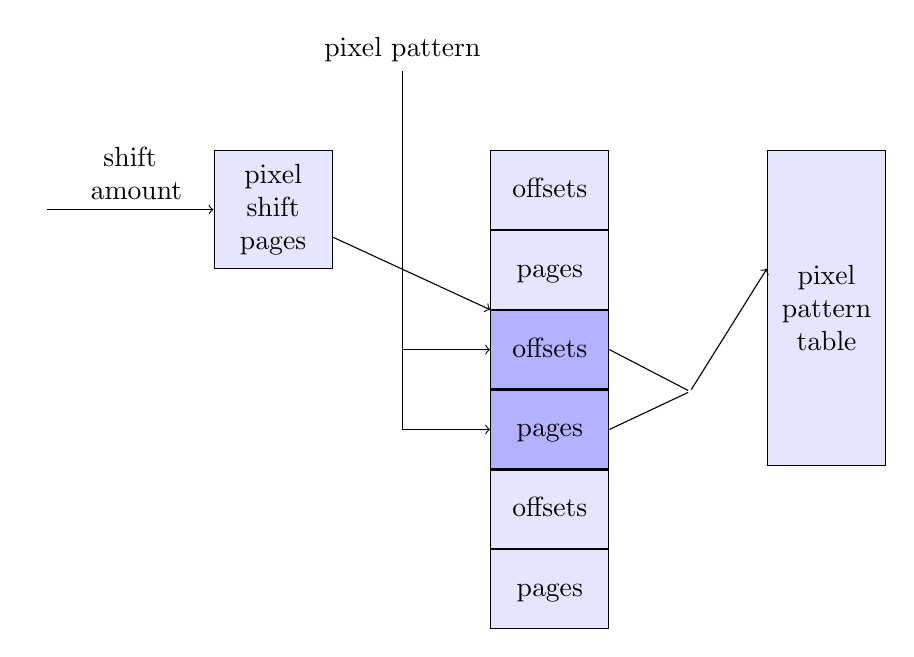
\begin{tikzpicture}
  [basicbox/.style={draw,rectangle,inner sep=0pt,minimum width=1.5cm,minimum height=1.5cm,fill=blue!10},
   pageoffsets/.style={basicbox,minimum height=1cm,text height=1.5ex,text depth=.25ex},
   multilinebox/.style={basicbox,text width=1cm,align=center}]
  \node (pixelshiftpages) at (0,0) [multilinebox] {pixel shift pages};
  \node (start) at (-3,0) {};
  \draw [->] (start) -- (pixelshiftpages) node [above,text width=1cm,align=center,midway] {shift amount};
  \node (offsets0) [pageoffsets,anchor=north,below right=0 and 2 of pixelshiftpages.north east] {offsets};
  \node (pages0) [pageoffsets,below=0 of offsets0.south] {pages};
  \node (offsets1) [pageoffsets,below=0 of pages0.south,fill=blue!30] {offsets};
  \node (pages1) [pageoffsets,below=0 of offsets1.south,fill=blue!30] {pages};
  \node (offsets2) [pageoffsets,below=0 of pages1.south] {offsets};
  \node (pages2) [pageoffsets,below=0 of offsets2.south] {pages};
  \draw [->] (pixelshiftpages) -- (offsets1.north west) {};
  \node (pixelpattern) [above left=1 and 0 of offsets0.north west] {pixel pattern};
  \draw [->] (pixelpattern.south) |- (offsets1.west) {};
  \draw [->] (pixelpattern.south) |- (pages1.west) {};
  \node (patterntable) [multilinebox,minimum height=4cm,text width=1.2cm,anchor=north west,below right=0 and 2 of offsets0.north east] {pixel pattern table};
  \node (join) [inner sep=0pt,below right=0 and 1 of offsets1.south east] {};
  \draw (offsets1.east) -- (join);
  \draw (pages1.east) -- (join);
  \draw [->] (join) -- ([yshift=5mm]patterntable.west);
\end{tikzpicture}
\vspace{1em}

The pixel pattern table is a table of every possible pattern of 7 consecutive pixels
spread out over two bytes. This table is 512 entries, each entry being two bytes.
A naive table would have redundancy. For example the pattern {\Tt{}0000100\nwendquote} starting
at column 0 is exactly the same as the pattern {\Tt{}0001000\nwendquote} starting at column 1.
This table eliminates that redundancy.

\nwenddocs{}\nwbegincode{10}\sublabel{NW1Xx3lK-1W8AJS-2}\nwmargintag{{\nwtagstyle{}\subpageref{NW1Xx3lK-1W8AJS-2}}}\moddef{tables~{\nwtagstyle{}\subpageref{NW1Xx3lK-1W8AJS-1}}}\plusendmoddef\nwstartdeflinemarkup\nwusesondefline{\\{NW1Xx3lK-1p0Y9w-1}}\nwprevnextdefs{NW1Xx3lK-1W8AJS-1}{NW1Xx3lK-1W8AJS-3}\nwenddeflinemarkup
    ORG     $A900
\nwlinkedidentc{PIXEL_PATTERN_TABLE}{NW1Xx3lK-1W8AJS-2}:
    INCLUDE "pixel_pattern_table.asm"
\nwindexdefn{\nwixident{PIXEL{\_}PATTERN{\_}TABLE}}{PIXEL:unPATTERN:unTABLE}{NW1Xx3lK-1W8AJS-2}\eatline
\nwused{\\{NW1Xx3lK-1p0Y9w-1}}\nwidentdefs{\\{{\nwixident{PIXEL{\_}PATTERN{\_}TABLE}}{PIXEL:unPATTERN:unTABLE}}}\nwendcode{}\nwbegindocs{11}\nwdocspar
Now we just need tables which index into {\Tt{}\nwlinkedidentq{PIXEL{\_}PATTERN{\_}TABLE}{NW1Xx3lK-1W8AJS-2}\nwendquote} for every
7-pixel pattern and shift value. This table works by having the page number
for the shifted pixel pattern at index {\Tt{}shift\ *\ 0x100\ +\ 0x80\ +\ pattern\nwendquote}
and the offset at index {\Tt{}shift\ *\ 0x100\ +\ pattern\nwendquote}.

\nwenddocs{}\nwbegincode{12}\sublabel{NW1Xx3lK-1W8AJS-3}\nwmargintag{{\nwtagstyle{}\subpageref{NW1Xx3lK-1W8AJS-3}}}\moddef{tables~{\nwtagstyle{}\subpageref{NW1Xx3lK-1W8AJS-1}}}\plusendmoddef\nwstartdeflinemarkup\nwusesondefline{\\{NW1Xx3lK-1p0Y9w-1}}\nwprevnextdefs{NW1Xx3lK-1W8AJS-2}{NW1Xx3lK-1W8AJS-4}\nwenddeflinemarkup
    ORG     $A200
\nwlinkedidentc{PIXEL_SHIFT_TABLE}{NW1Xx3lK-1W8AJS-3}:
    INCLUDE "pixel_shift_table.asm"
\nwindexdefn{\nwixident{PIXEL{\_}SHIFT{\_}TABLE}}{PIXEL:unSHIFT:unTABLE}{NW1Xx3lK-1W8AJS-3}\eatline
\nwused{\\{NW1Xx3lK-1p0Y9w-1}}\nwidentdefs{\\{{\nwixident{PIXEL{\_}SHIFT{\_}TABLE}}{PIXEL:unSHIFT:unTABLE}}}\nwendcode{}\nwbegindocs{13}\nwdocspar
Rather than multiplying the shift value by {\Tt{}0x100\nwendquote}, we instead define
another table which holds the page numbers for the shift tables for each
shift value.

\nwenddocs{}\nwbegincode{14}\sublabel{NW1Xx3lK-1W8AJS-4}\nwmargintag{{\nwtagstyle{}\subpageref{NW1Xx3lK-1W8AJS-4}}}\moddef{tables~{\nwtagstyle{}\subpageref{NW1Xx3lK-1W8AJS-1}}}\plusendmoddef\nwstartdeflinemarkup\nwusesondefline{\\{NW1Xx3lK-1p0Y9w-1}}\nwprevnextdefs{NW1Xx3lK-1W8AJS-3}{NW1Xx3lK-1W8AJS-5}\nwenddeflinemarkup
    ORG     $84C1
\nwlinkedidentc{PIXEL_SHIFT_PAGES}{NW1Xx3lK-1W8AJS-4}:
    HEX     A2 A3 A4 A5 A6 A7 A8
\nwindexdefn{\nwixident{PIXEL{\_}SHIFT{\_}PAGES}}{PIXEL:unSHIFT:unPAGES}{NW1Xx3lK-1W8AJS-4}\eatline
\nwused{\\{NW1Xx3lK-1p0Y9w-1}}\nwidentdefs{\\{{\nwixident{PIXEL{\_}SHIFT{\_}PAGES}}{PIXEL:unSHIFT:unPAGES}}}\nwendcode{}\nwbegindocs{15}\nwdocspar
So we can get shifted pixels by indexing into all these tables.

Now we can define a routine that will take a sprite number and a pixel shift
amount, and write the shifted pixel data into the {\Tt{}\nwlinkedidentq{BLOCK{\_}DATA}{NW1Xx3lK-10jlgu-2}\nwendquote} area. The
routine first shifts the first byte of the sprite into a two-byte area. Then
it shifts the second byte of the sprite, and combines that two-byte result
with the first. Thus, we shift two bytes of sprite data into a three-byte
result.

\begin{center}
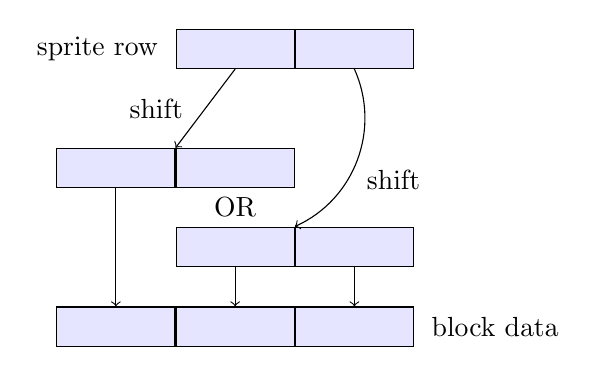
\begin{tikzpicture}
  [basicbox/.style={draw,rectangle,inner sep=0pt,minimum width=1.5cm,minimum height=0.5cm,fill=blue!10}]
  \node (spriterowbyte0) at (0,0) [basicbox] {};
  \node (spriterowbyte1) [basicbox,right=0 of spriterowbyte0.east] {};
  \node (spriterowlabel) [left=0.1 of spriterowbyte0.west] {sprite row};
  \node (shifted0byte0) [basicbox,below left=1 and 0 of spriterowbyte0.south west] {};
  \node (shifted0byte1) [basicbox,right=0 of shifted0byte0.east] {};
  \node (shifted1byte0) [basicbox,below right=2 and 0 of spriterowbyte0.south west] {};
  \node (shifted1byte1) [basicbox,right=0 of shifted1byte0.east] {};
  \node (orlabel) [below=0 of shifted0byte1] {OR};
  \draw [->] (spriterowbyte0.south) -- (shifted0byte0.north east)
    node [left,text width=1cm,align=center,midway] {shift};
  \draw [->] (spriterowbyte1.south) to [auto, bend left=45] node {shift} (shifted1byte0.north east);
  \node (result0) [basicbox,below left=0.5 and 0 of shifted1byte0.south west] {};
  \node (result1) [basicbox,right=0 of result0.east] {};
  \node (result2) [basicbox,right=0 of result1.east] {};
  \draw [->] (shifted0byte0) -- (result0) {};
  \draw [->] (shifted1byte0) -- (result1) {};
  \draw [->] (shifted1byte1) -- (result2) {};
  \node (blocklabel) [right=0.1 of result2.east] {block data};
\end{tikzpicture}
\end{center}

Rather than load addresses from the tables and store them, the routine
modifies its own instructions with those addresses.

\nwenddocs{}\nwbegincode{16}\sublabel{NW1Xx3lK-10jlgu-3}\nwmargintag{{\nwtagstyle{}\subpageref{NW1Xx3lK-10jlgu-3}}}\moddef{defines~{\nwtagstyle{}\subpageref{NW1Xx3lK-10jlgu-1}}}\plusendmoddef\nwstartdeflinemarkup\nwusesondefline{\\{NW1Xx3lK-1p0Y9w-1}}\nwprevnextdefs{NW1Xx3lK-10jlgu-2}{NW1Xx3lK-10jlgu-4}\nwenddeflinemarkup
    ORG     $1D
\nwlinkedidentc{ROW_COUNT}{NW1Xx3lK-10jlgu-3}       DS      1
\nwlinkedidentc{SPRITE_NUM}{NW1Xx3lK-10jlgu-3}      DS      1
\nwindexdefn{\nwixident{ROW{\_}COUNT}}{ROW:unCOUNT}{NW1Xx3lK-10jlgu-3}\nwindexdefn{\nwixident{SPRITE{\_}NUM}}{SPRITE:unNUM}{NW1Xx3lK-10jlgu-3}\eatline
\nwused{\\{NW1Xx3lK-1p0Y9w-1}}\nwidentdefs{\\{{\nwixident{ROW{\_}COUNT}}{ROW:unCOUNT}}\\{{\nwixident{SPRITE{\_}NUM}}{SPRITE:unNUM}}}\nwendcode{}\nwbegindocs{17}\nwdocspar
\nwenddocs{}\nwbegincode{18}\sublabel{NW1Xx3lK-8jv1b-2}\nwmargintag{{\nwtagstyle{}\subpageref{NW1Xx3lK-8jv1b-2}}}\moddef{routines~{\nwtagstyle{}\subpageref{NW1Xx3lK-8jv1b-1}}}\plusendmoddef\nwstartdeflinemarkup\nwusesondefline{\\{NW1Xx3lK-1p0Y9w-1}}\nwprevnextdefs{NW1Xx3lK-8jv1b-1}{NW1Xx3lK-8jv1b-3}\nwenddeflinemarkup
    ORG     $8438
\nwlinkedidentc{COMPUTE_SHIFTED_SPRITE}{NW1Xx3lK-8jv1b-2}:
    SUBROUTINE
    ; Enter routine with X set to pixel shift amount and
    ; \nwlinkedidentc{SPRITE_NUM}{NW1Xx3lK-10jlgu-3} containing the sprite number to read.

.offset_table       EQU $A000               ; Target addresses in read
.page_table         EQU $A080               ; instructions. The only truly
.shift_ptr_byte0    EQU $A000               ; necessary value here is the
.shift_ptr_byte1    EQU $A000               ; 0x80 in .shift_ptr_byte0.

    LDA     #$0B                            ; 11 rows
    STA     \nwlinkedidentc{ROW_COUNT}{NW1Xx3lK-10jlgu-3}
    LDA     #<\nwlinkedidentc{SPRITE_DATA}{NW1Xx3lK-1W8AJS-1}
    STA     \nwlinkedidentc{TMP_PTR}{NW1Xx3lK-10jlgu-1}
    LDA     #>\nwlinkedidentc{SPRITE_DATA}{NW1Xx3lK-1W8AJS-1}
    STA     \nwlinkedidentc{TMP_PTR}{NW1Xx3lK-10jlgu-1}+1                       ; \nwlinkedidentc{TMP_PTR}{NW1Xx3lK-10jlgu-1} = \nwlinkedidentc{SPRITE_DATA}{NW1Xx3lK-1W8AJS-1}
    LDA     \nwlinkedidentc{PIXEL_SHIFT_PAGES}{NW1Xx3lK-1W8AJS-4},X 
    STA     .rd_offset_table + 2
    STA     .rd_page_table + 2
    STA     .rd_offset_table2 + 2
    STA     .rd_page_table2 + 2             ; Fix up pages in lookup instructions
                                            ; based on shift amount (X).

    LDX     #$00                            ; X is the offset into \nwlinkedidentc{BLOCK_DATA}{NW1Xx3lK-10jlgu-2}.

.loop:                                      ; === LOOP === (over all 11 rows)
    LDY     \nwlinkedidentc{SPRITE_NUM}{NW1Xx3lK-10jlgu-3}
    LDA     (\nwlinkedidentc{TMP_PTR}{NW1Xx3lK-10jlgu-1}),Y 
    TAY                                     ; Get sprite pixel data.

.rd_offset_table:
    LDA     .offset_table,Y                 ; Load offset for shift amount.
    STA     .rd_shift_ptr_byte0 + 1
    CLC
    ADC     #$01
    STA     .rd_shift_ptr_byte1 + 1         ; Fix up instruction offsets with it.
.rd_page_table:
    LDA     .page_table,Y                   ; Load page for shift amount.
    STA     .rd_shift_ptr_byte0 + 2
    STA     .rd_shift_ptr_byte1 + 2         ; Fix up instruction page with it.

.rd_shift_ptr_byte0:
    LDA     .shift_ptr_byte0                ; Read shifted pixel data byte 0
    STA     \nwlinkedidentc{BLOCK_DATA}{NW1Xx3lK-10jlgu-2},X                    ; and store in block data byte 0.
.rd_shift_ptr_byte1:
    LDA     .shift_ptr_byte1                ; Read shifted pixel data byte 1
    STA     \nwlinkedidentc{BLOCK_DATA}{NW1Xx3lK-10jlgu-2}+1,X                  ; and store in block data byte 1.

    LDA     \nwlinkedidentc{TMP_PTR}{NW1Xx3lK-10jlgu-1}
    CLC
    ADC     #$68
    STA     \nwlinkedidentc{TMP_PTR}{NW1Xx3lK-10jlgu-1}
    LDA     \nwlinkedidentc{TMP_PTR}{NW1Xx3lK-10jlgu-1}+1
    ADC     #$00
    STA     \nwlinkedidentc{TMP_PTR}{NW1Xx3lK-10jlgu-1}+1                       ; \nwlinkedidentc{TMP_PTR}{NW1Xx3lK-10jlgu-1}++

    ; Now basically do the same thing with the second sprite byte

    LDY     \nwlinkedidentc{SPRITE_NUM}{NW1Xx3lK-10jlgu-3}
    LDA     (\nwlinkedidentc{TMP_PTR}{NW1Xx3lK-10jlgu-1}),Y 
    TAY                                     ; Get sprite pixel data.

.rd_offset_table2:
    LDA     .offset_table,Y                 ; Load offset for shift amount.
    STA     .rd_shift_ptr2_byte0 + 1
    CLC
    ADC     #$01
    STA     .rd_shift_ptr2_byte1 + 1        ; Fix up instruction offsets with it.
.rd_page_table2:
    LDA     .page_table,Y                   ; Load page for shift amount.
    STA     .rd_shift_ptr2_byte0 + 2
    STA     .rd_shift_ptr2_byte1 + 2        ; Fix up instruction page with it.

.rd_shift_ptr2_byte0:
    LDA     .shift_ptr_byte0                ; Read shifted pixel data byte 0
    ORA     \nwlinkedidentc{BLOCK_DATA}{NW1Xx3lK-10jlgu-2}+1,X                  ; OR with previous block data byte 1
    STA     \nwlinkedidentc{BLOCK_DATA}{NW1Xx3lK-10jlgu-2}+1,X                  ; and store in block data byte 1.
.rd_shift_ptr2_byte1:
    LDA     .shift_ptr_byte1                ; Read shifted pixel data byte 1
    STA     \nwlinkedidentc{BLOCK_DATA}{NW1Xx3lK-10jlgu-2}+2,X                  ; and store in block data byte 2.

    LDA     \nwlinkedidentc{TMP_PTR}{NW1Xx3lK-10jlgu-1}
    CLC
    ADC     #$68
    STA     \nwlinkedidentc{TMP_PTR}{NW1Xx3lK-10jlgu-1}
    LDA     \nwlinkedidentc{TMP_PTR}{NW1Xx3lK-10jlgu-1}+1
    ADC     #$00
    STA     \nwlinkedidentc{TMP_PTR}{NW1Xx3lK-10jlgu-1}+1                       ; \nwlinkedidentc{TMP_PTR}{NW1Xx3lK-10jlgu-1}++

    INX
    INX
    INX                                     ; X += 3
    DEC     \nwlinkedidentc{ROW_COUNT}{NW1Xx3lK-10jlgu-3}                       ; \nwlinkedidentc{ROW_COUNT}{NW1Xx3lK-10jlgu-3}--
    BNE     .loop                           ; loop while \nwlinkedidentc{ROW_COUNT}{NW1Xx3lK-10jlgu-3} > 0
    RTS
\nwindexdefn{\nwixident{COMPUTE{\_}SHIFTED{\_}SPRITE}}{COMPUTE:unSHIFTED:unSPRITE}{NW1Xx3lK-8jv1b-2}\eatline
\nwused{\\{NW1Xx3lK-1p0Y9w-1}}\nwidentdefs{\\{{\nwixident{COMPUTE{\_}SHIFTED{\_}SPRITE}}{COMPUTE:unSHIFTED:unSPRITE}}}\nwidentuses{\\{{\nwixident{BLOCK{\_}DATA}}{BLOCK:unDATA}}\\{{\nwixident{PIXEL{\_}SHIFT{\_}PAGES}}{PIXEL:unSHIFT:unPAGES}}\\{{\nwixident{ROW{\_}COUNT}}{ROW:unCOUNT}}\\{{\nwixident{SPRITE{\_}DATA}}{SPRITE:unDATA}}\\{{\nwixident{SPRITE{\_}NUM}}{SPRITE:unNUM}}\\{{\nwixident{TMP{\_}PTR}}{TMP:unPTR}}}\nwindexuse{\nwixident{BLOCK{\_}DATA}}{BLOCK:unDATA}{NW1Xx3lK-8jv1b-2}\nwindexuse{\nwixident{PIXEL{\_}SHIFT{\_}PAGES}}{PIXEL:unSHIFT:unPAGES}{NW1Xx3lK-8jv1b-2}\nwindexuse{\nwixident{ROW{\_}COUNT}}{ROW:unCOUNT}{NW1Xx3lK-8jv1b-2}\nwindexuse{\nwixident{SPRITE{\_}DATA}}{SPRITE:unDATA}{NW1Xx3lK-8jv1b-2}\nwindexuse{\nwixident{SPRITE{\_}NUM}}{SPRITE:unNUM}{NW1Xx3lK-8jv1b-2}\nwindexuse{\nwixident{TMP{\_}PTR}}{TMP:unPTR}{NW1Xx3lK-8jv1b-2}\nwendcode{}\nwbegindocs{19}\nwdocspar
\section{Memory mapped graphics}

Within a screen row, consecutive bytes map to consecutive pixels. However, rows
themselves are not consecutive in memory.

To make it easy to convert a row number from 0 to 191 to a base address, Lode Runner has
a table and a routine to use that table.

\nwenddocs{}\nwbegincode{20}\sublabel{NW1Xx3lK-1W8AJS-5}\nwmargintag{{\nwtagstyle{}\subpageref{NW1Xx3lK-1W8AJS-5}}}\moddef{tables~{\nwtagstyle{}\subpageref{NW1Xx3lK-1W8AJS-1}}}\plusendmoddef\nwstartdeflinemarkup\nwusesondefline{\\{NW1Xx3lK-1p0Y9w-1}}\nwprevnextdefs{NW1Xx3lK-1W8AJS-4}{NW1Xx3lK-1W8AJS-6}\nwenddeflinemarkup
    ORG     $1A85
\nwlinkedidentc{ROW_TO_OFFSET_LO}{NW1Xx3lK-1W8AJS-5}:
    INCLUDE "row_to_offset_lo_table.asm"
\nwlinkedidentc{ROW_TO_OFFSET_HI}{NW1Xx3lK-1W8AJS-5}:
    INCLUDE "row_to_offset_hi_table.asm"
\nwindexdefn{\nwixident{ROW{\_}TO{\_}OFFSET{\_}LO}}{ROW:unTO:unOFFSET:unLO}{NW1Xx3lK-1W8AJS-5}\nwindexdefn{\nwixident{ROW{\_}TO{\_}OFFSET{\_}HI}}{ROW:unTO:unOFFSET:unHI}{NW1Xx3lK-1W8AJS-5}\eatline
\nwused{\\{NW1Xx3lK-1p0Y9w-1}}\nwidentdefs{\\{{\nwixident{ROW{\_}TO{\_}OFFSET{\_}HI}}{ROW:unTO:unOFFSET:unHI}}\\{{\nwixident{ROW{\_}TO{\_}OFFSET{\_}LO}}{ROW:unTO:unOFFSET:unLO}}}\nwendcode{}\nwbegindocs{21}\nwdocspar
\nwenddocs{}\nwbegincode{22}\sublabel{NW1Xx3lK-10jlgu-4}\nwmargintag{{\nwtagstyle{}\subpageref{NW1Xx3lK-10jlgu-4}}}\moddef{defines~{\nwtagstyle{}\subpageref{NW1Xx3lK-10jlgu-1}}}\plusendmoddef\nwstartdeflinemarkup\nwusesondefline{\\{NW1Xx3lK-1p0Y9w-1}}\nwprevnextdefs{NW1Xx3lK-10jlgu-3}{NW1Xx3lK-10jlgu-5}\nwenddeflinemarkup
\nwlinkedidentc{ROW_ADDR}{NW1Xx3lK-10jlgu-4}        EQU     $0C     ; 2 bytes
\nwlinkedidentc{ROW_ADDR2}{NW1Xx3lK-10jlgu-4}       EQU     $0E     ; 2 bytes
\nwlinkedidentc{HGR_PAGE}{NW1Xx3lK-10jlgu-4}        EQU     $1F     ; 0x20 for HGR1, 0x40 for HGR2
\nwindexdefn{\nwixident{ROW{\_}ADDR}}{ROW:unADDR}{NW1Xx3lK-10jlgu-4}\nwindexdefn{\nwixident{ROW{\_}ADDR2}}{ROW:unADDR2}{NW1Xx3lK-10jlgu-4}\nwindexdefn{\nwixident{HGR{\_}PAGE}}{HGR:unPAGE}{NW1Xx3lK-10jlgu-4}\eatline
\nwused{\\{NW1Xx3lK-1p0Y9w-1}}\nwidentdefs{\\{{\nwixident{HGR{\_}PAGE}}{HGR:unPAGE}}\\{{\nwixident{ROW{\_}ADDR}}{ROW:unADDR}}\\{{\nwixident{ROW{\_}ADDR2}}{ROW:unADDR2}}}\nwendcode{}\nwbegindocs{23}\nwdocspar
\nwenddocs{}\nwbegincode{24}\sublabel{NW1Xx3lK-8jv1b-3}\nwmargintag{{\nwtagstyle{}\subpageref{NW1Xx3lK-8jv1b-3}}}\moddef{routines~{\nwtagstyle{}\subpageref{NW1Xx3lK-8jv1b-1}}}\plusendmoddef\nwstartdeflinemarkup\nwusesondefline{\\{NW1Xx3lK-1p0Y9w-1}}\nwprevnextdefs{NW1Xx3lK-8jv1b-2}{NW1Xx3lK-8jv1b-4}\nwenddeflinemarkup
    ORG     $7A31
\nwlinkedidentc{ROW_TO_ADDR}{NW1Xx3lK-8jv1b-3}:
    SUBROUTINE
    ; Enter routine with Y set to row. Base address
    ; (for column 0) will be placed in \nwlinkedidentc{ROW_ADDR}{NW1Xx3lK-10jlgu-4}.

    LDA     \nwlinkedidentc{ROW_TO_OFFSET_LO}{NW1Xx3lK-1W8AJS-5},Y 
    STA     \nwlinkedidentc{ROW_ADDR}{NW1Xx3lK-10jlgu-4}
    LDA     \nwlinkedidentc{ROW_TO_OFFSET_HI}{NW1Xx3lK-1W8AJS-5},Y 
    ORA     \nwlinkedidentc{HGR_PAGE}{NW1Xx3lK-10jlgu-4}
    STA     \nwlinkedidentc{ROW_ADDR}{NW1Xx3lK-10jlgu-4}+1
    RTS
\nwindexdefn{\nwixident{ROW{\_}TO{\_}ADDR}}{ROW:unTO:unADDR}{NW1Xx3lK-8jv1b-3}\eatline
\nwused{\\{NW1Xx3lK-1p0Y9w-1}}\nwidentdefs{\\{{\nwixident{ROW{\_}TO{\_}ADDR}}{ROW:unTO:unADDR}}}\nwidentuses{\\{{\nwixident{HGR{\_}PAGE}}{HGR:unPAGE}}\\{{\nwixident{ROW{\_}ADDR}}{ROW:unADDR}}\\{{\nwixident{ROW{\_}TO{\_}OFFSET{\_}HI}}{ROW:unTO:unOFFSET:unHI}}\\{{\nwixident{ROW{\_}TO{\_}OFFSET{\_}LO}}{ROW:unTO:unOFFSET:unLO}}}\nwindexuse{\nwixident{HGR{\_}PAGE}}{HGR:unPAGE}{NW1Xx3lK-8jv1b-3}\nwindexuse{\nwixident{ROW{\_}ADDR}}{ROW:unADDR}{NW1Xx3lK-8jv1b-3}\nwindexuse{\nwixident{ROW{\_}TO{\_}OFFSET{\_}HI}}{ROW:unTO:unOFFSET:unHI}{NW1Xx3lK-8jv1b-3}\nwindexuse{\nwixident{ROW{\_}TO{\_}OFFSET{\_}LO}}{ROW:unTO:unOFFSET:unLO}{NW1Xx3lK-8jv1b-3}\nwendcode{}\nwbegindocs{25}\nwdocspar
There's also a routine to load the address for both page 1 and page 2.

\nwenddocs{}\nwbegincode{26}\sublabel{NW1Xx3lK-8jv1b-4}\nwmargintag{{\nwtagstyle{}\subpageref{NW1Xx3lK-8jv1b-4}}}\moddef{routines~{\nwtagstyle{}\subpageref{NW1Xx3lK-8jv1b-1}}}\plusendmoddef\nwstartdeflinemarkup\nwusesondefline{\\{NW1Xx3lK-1p0Y9w-1}}\nwprevnextdefs{NW1Xx3lK-8jv1b-3}{NW1Xx3lK-8jv1b-5}\nwenddeflinemarkup
    ORG     $7A3E
\nwlinkedidentc{ROW_TO_ADDR_FOR_BOTH_PAGES}{NW1Xx3lK-8jv1b-4}:
    SUBROUTINE
    ; Enter routine with Y set to row. Base address
    ; (for column 0) will be placed in \nwlinkedidentc{ROW_ADDR}{NW1Xx3lK-10jlgu-4} (for page 1)
    ; and \nwlinkedidentc{ROW_ADDR2}{NW1Xx3lK-10jlgu-4} (for page 2).

    LDA     \nwlinkedidentc{ROW_TO_OFFSET_LO}{NW1Xx3lK-1W8AJS-5},Y 
    STA     \nwlinkedidentc{ROW_ADDR}{NW1Xx3lK-10jlgu-4}
    STA     \nwlinkedidentc{ROW_ADDR2}{NW1Xx3lK-10jlgu-4}
    LDA     \nwlinkedidentc{ROW_TO_OFFSET_HI}{NW1Xx3lK-1W8AJS-5},Y 
    ORA     #$20
    STA     \nwlinkedidentc{ROW_ADDR}{NW1Xx3lK-10jlgu-4}+1
    EOR     #$60
    STA     \nwlinkedidentc{ROW_ADDR2}{NW1Xx3lK-10jlgu-4}+1
    RTS
\nwindexdefn{\nwixident{ROW{\_}TO{\_}ADDR{\_}FOR{\_}BOTH{\_}PAGES}}{ROW:unTO:unADDR:unFOR:unBOTH:unPAGES}{NW1Xx3lK-8jv1b-4}\eatline
\nwused{\\{NW1Xx3lK-1p0Y9w-1}}\nwidentdefs{\\{{\nwixident{ROW{\_}TO{\_}ADDR{\_}FOR{\_}BOTH{\_}PAGES}}{ROW:unTO:unADDR:unFOR:unBOTH:unPAGES}}}\nwidentuses{\\{{\nwixident{ROW{\_}ADDR}}{ROW:unADDR}}\\{{\nwixident{ROW{\_}ADDR2}}{ROW:unADDR2}}\\{{\nwixident{ROW{\_}TO{\_}OFFSET{\_}HI}}{ROW:unTO:unOFFSET:unHI}}\\{{\nwixident{ROW{\_}TO{\_}OFFSET{\_}LO}}{ROW:unTO:unOFFSET:unLO}}}\nwindexuse{\nwixident{ROW{\_}ADDR}}{ROW:unADDR}{NW1Xx3lK-8jv1b-4}\nwindexuse{\nwixident{ROW{\_}ADDR2}}{ROW:unADDR2}{NW1Xx3lK-8jv1b-4}\nwindexuse{\nwixident{ROW{\_}TO{\_}OFFSET{\_}HI}}{ROW:unTO:unOFFSET:unHI}{NW1Xx3lK-8jv1b-4}\nwindexuse{\nwixident{ROW{\_}TO{\_}OFFSET{\_}LO}}{ROW:unTO:unOFFSET:unLO}{NW1Xx3lK-8jv1b-4}\nwendcode{}\nwbegindocs{27}\nwdocspar

Lode Runner's screens are organized into 28 sprites across by 17 sprites
down. To convert between sprite coordinates and screen coordinates and vice-versa, we
use tables and lookup routines. Each sprite is 10 pixels across by 11 pixels down.

\nwenddocs{}\nwbegincode{28}\sublabel{NW1Xx3lK-1W8AJS-6}\nwmargintag{{\nwtagstyle{}\subpageref{NW1Xx3lK-1W8AJS-6}}}\moddef{tables~{\nwtagstyle{}\subpageref{NW1Xx3lK-1W8AJS-1}}}\plusendmoddef\nwstartdeflinemarkup\nwusesondefline{\\{NW1Xx3lK-1p0Y9w-1}}\nwprevnextdefs{NW1Xx3lK-1W8AJS-5}{NW1Xx3lK-1W8AJS-7}\nwenddeflinemarkup
    ORG     $1C35
\nwlinkedidentc{HALF_SCREEN_COL_TABLE}{NW1Xx3lK-1W8AJS-6}:
    ; 28 cols of 5 double-pixels each
    HEX     00 05 0a 0f 14 19 1e 23 28 2d 32 37 3c 41 46 4b
    HEX     50 55 5a 5f 64 69 6e 73 78 7d 82 87
\nwlinkedidentc{SCREEN_ROW_TABLE}{NW1Xx3lK-1W8AJS-6}:
    ; 17 rows of 11 pixels each
    HEX     00 0B 16 21 2C 37 42 4D 58 63 6E 79 84 8F 9A A5
    HEX     B5
\nwlinkedidentc{COL_BYTE_TABLE}{NW1Xx3lK-1W8AJS-6}:
    ; Byte number
    HEX     00 01 02 04 05 07 08 0A 0B 0C 0E 0F 11 12 14 15
    HEX     16 18 19 1B 1C 1E 1F 20 22 23 25 26
\nwlinkedidentc{COL_SHIFT_TABLE}{NW1Xx3lK-1W8AJS-6}:
    ; Right shift amount
    HEX     00 03 06 02 05 01 04 00 03 06 02 05 01 04 00 03
    HEX     06 02 05 01 04 00 03 06 02 05 01 04
\nwlinkedidentc{HALF_SCREEN_COL_BYTE_TABLE}{NW1Xx3lK-1W8AJS-6}:
    HEX     00 00 00 00 01 01 01 02 02 02 02 03 03 03 04 04
    HEX     04 04 05 05 05 06 06 06 06 07 07 07 08 08 08 08
    HEX     09 09 09 0A 0A 0A 0A 0B 0B 0B 0C 0C 0C 0C 0D 0D
    HEX     0D 0E 0E 0E 0E 0F 0F 0F 10 10 10 10 11 11 11 12
    HEX     12 12 12 13 13 13 14 14 14 14 15 15 15 16 16 16
    HEX     16 17 17 17 18 18 18 18 19 19 19 1A 1A 1A 1A 1B
    HEX     1B 1B 1C 1C 1C 1C 1D 1D 1D 1E 1E 1E 1E 1F 1F 1F
    HEX     20 20 20 20 21 21 21 22 22 22 22 23 23 23 24 24
    HEX     24 24 25 25 25 26 26 26 26 27 27 27
\nwlinkedidentc{HALF_SCREEN_COL_SHIFT_TABLE}{NW1Xx3lK-1W8AJS-6}:
    HEX     00 02 04 06 01 03 05 00 02 04 06 01 03 05 00 02
    HEX     04 06 01 03 05 00 02 04 06 01 03 05 00 02 04 06
    HEX     01 03 05 00 02 04 06 01 03 05 00 02 04 06 01 03
    HEX     05 00 02 04 06 01 03 05 00 02 04 06 01 03 05 00
    HEX     02 04 06 01 03 05 00 02 04 06 01 03 05 00 02 04
    HEX     06 01 03 05 00 02 04 06 01 03 05 00 02 04 06 01
    HEX     03 05 00 02 04 06 01 03 05 00 02 04 06 01 03 05
    HEX     00 02 04 06 01 03 05 00 02 04 06 01 03 05 00 02
    HEX     04 06 01 03 05 00 02 04 06 01 03 05
\nwindexdefn{\nwixident{SCREEN{\_}ROW{\_}TABLE}}{SCREEN:unROW:unTABLE}{NW1Xx3lK-1W8AJS-6}\nwindexdefn{\nwixident{COL{\_}BYTE{\_}TABLE}}{COL:unBYTE:unTABLE}{NW1Xx3lK-1W8AJS-6}\nwindexdefn{\nwixident{HALF{\_}SCREEN{\_}COL{\_}TABLE}}{HALF:unSCREEN:unCOL:unTABLE}{NW1Xx3lK-1W8AJS-6}\nwindexdefn{\nwixident{COL{\_}SHIFT{\_}TABLE}}{COL:unSHIFT:unTABLE}{NW1Xx3lK-1W8AJS-6}\nwindexdefn{\nwixident{HALF{\_}SCREEN{\_}COL{\_}BYTE{\_}TABLE}}{HALF:unSCREEN:unCOL:unBYTE:unTABLE}{NW1Xx3lK-1W8AJS-6}\nwindexdefn{\nwixident{HALF{\_}SCREEN{\_}COL{\_}SHIFT{\_}TABLE}}{HALF:unSCREEN:unCOL:unSHIFT:unTABLE}{NW1Xx3lK-1W8AJS-6}\eatline
\nwused{\\{NW1Xx3lK-1p0Y9w-1}}\nwidentdefs{\\{{\nwixident{COL{\_}BYTE{\_}TABLE}}{COL:unBYTE:unTABLE}}\\{{\nwixident{COL{\_}SHIFT{\_}TABLE}}{COL:unSHIFT:unTABLE}}\\{{\nwixident{HALF{\_}SCREEN{\_}COL{\_}BYTE{\_}TABLE}}{HALF:unSCREEN:unCOL:unBYTE:unTABLE}}\\{{\nwixident{HALF{\_}SCREEN{\_}COL{\_}SHIFT{\_}TABLE}}{HALF:unSCREEN:unCOL:unSHIFT:unTABLE}}\\{{\nwixident{HALF{\_}SCREEN{\_}COL{\_}TABLE}}{HALF:unSCREEN:unCOL:unTABLE}}\\{{\nwixident{SCREEN{\_}ROW{\_}TABLE}}{SCREEN:unROW:unTABLE}}}\nwendcode{}\nwbegindocs{29}\nwdocspar
Here is the routine to return the screen coordinates for the given sprite coordinates.
The reason that {\Tt{}\nwlinkedidentq{GET{\_}SCREEN{\_}COORDS{\_}FOR}{NW1Xx3lK-8jv1b-5}\nwendquote} returns half the screen column coordinate
is that otherwise the screen column coordinate wouldn't fit in a register.

\nwenddocs{}\nwbegincode{30}\sublabel{NW1Xx3lK-8jv1b-5}\nwmargintag{{\nwtagstyle{}\subpageref{NW1Xx3lK-8jv1b-5}}}\moddef{routines~{\nwtagstyle{}\subpageref{NW1Xx3lK-8jv1b-1}}}\plusendmoddef\nwstartdeflinemarkup\nwusesondefline{\\{NW1Xx3lK-1p0Y9w-1}}\nwprevnextdefs{NW1Xx3lK-8jv1b-4}{NW1Xx3lK-8jv1b-6}\nwenddeflinemarkup
    ORG     $885D
\nwlinkedidentc{GET_SCREEN_COORDS_FOR}{NW1Xx3lK-8jv1b-5}:
    SUBROUTINE
    ; Enter routine with Y set to sprite row (0-16) and
    ; X set to sprite column (0-27). On return, Y will be set to
    ; screen row, and X is set to half screen column.

    LDA     \nwlinkedidentc{SCREEN_ROW_TABLE}{NW1Xx3lK-1W8AJS-6},Y 
    PHA
    LDA     \nwlinkedidentc{HALF_SCREEN_COL_TABLE}{NW1Xx3lK-1W8AJS-6},X 
    TAX                         ; X = \nwlinkedidentc{HALF_SCREEN_COL_TABLE}{NW1Xx3lK-1W8AJS-6}[X]
    PLA
    TAY                         ; Y = \nwlinkedidentc{SCREEN_ROW_TABLE}{NW1Xx3lK-1W8AJS-6}[Y]
    RTS
\nwindexdefn{\nwixident{GET{\_}SCREEN{\_}COORDS{\_}FOR}}{GET:unSCREEN:unCOORDS:unFOR}{NW1Xx3lK-8jv1b-5}\eatline
\nwused{\\{NW1Xx3lK-1p0Y9w-1}}\nwidentdefs{\\{{\nwixident{GET{\_}SCREEN{\_}COORDS{\_}FOR}}{GET:unSCREEN:unCOORDS:unFOR}}}\nwidentuses{\\{{\nwixident{HALF{\_}SCREEN{\_}COL{\_}TABLE}}{HALF:unSCREEN:unCOL:unTABLE}}\\{{\nwixident{SCREEN{\_}ROW{\_}TABLE}}{SCREEN:unROW:unTABLE}}}\nwindexuse{\nwixident{HALF{\_}SCREEN{\_}COL{\_}TABLE}}{HALF:unSCREEN:unCOL:unTABLE}{NW1Xx3lK-8jv1b-5}\nwindexuse{\nwixident{SCREEN{\_}ROW{\_}TABLE}}{SCREEN:unROW:unTABLE}{NW1Xx3lK-8jv1b-5}\nwendcode{}\nwbegindocs{31}\nwdocspar
This routine takes a sprite column and converts it to
the memory-mapped byte offset and right-shift amount.

\nwenddocs{}\nwbegincode{32}\sublabel{NW1Xx3lK-8jv1b-6}\nwmargintag{{\nwtagstyle{}\subpageref{NW1Xx3lK-8jv1b-6}}}\moddef{routines~{\nwtagstyle{}\subpageref{NW1Xx3lK-8jv1b-1}}}\plusendmoddef\nwstartdeflinemarkup\nwusesondefline{\\{NW1Xx3lK-1p0Y9w-1}}\nwprevnextdefs{NW1Xx3lK-8jv1b-5}{NW1Xx3lK-8jv1b-7}\nwenddeflinemarkup
    ORG     $8868
\nwlinkedidentc{GET_BYTE_AND_SHIFT_FOR_COL}{NW1Xx3lK-8jv1b-6}:
    SUBROUTINE
    ; Enter routine with X set to sprite column. On
    ; return, A will be set to screen column byte number
    ; and X will be set to an additional right shift amount.

    LDA     \nwlinkedidentc{COL_BYTE_TABLE}{NW1Xx3lK-1W8AJS-6},X 
    PHA                         ; A = \nwlinkedidentc{COL_BYTE_TABLE}{NW1Xx3lK-1W8AJS-6}[X]
    LDA     \nwlinkedidentc{COL_SHIFT_TABLE}{NW1Xx3lK-1W8AJS-6},X 
    TAX                         ; X = \nwlinkedidentc{COL_SHIFT_TABLE}{NW1Xx3lK-1W8AJS-6}[X]
    PLA
    RTS
\nwindexdefn{\nwixident{GET{\_}BYTE{\_}AND{\_}SHIFT{\_}FOR{\_}COL}}{GET:unBYTE:unAND:unSHIFT:unFOR:unCOL}{NW1Xx3lK-8jv1b-6}\eatline
\nwused{\\{NW1Xx3lK-1p0Y9w-1}}\nwidentdefs{\\{{\nwixident{GET{\_}BYTE{\_}AND{\_}SHIFT{\_}FOR{\_}COL}}{GET:unBYTE:unAND:unSHIFT:unFOR:unCOL}}}\nwidentuses{\\{{\nwixident{COL{\_}BYTE{\_}TABLE}}{COL:unBYTE:unTABLE}}\\{{\nwixident{COL{\_}SHIFT{\_}TABLE}}{COL:unSHIFT:unTABLE}}}\nwindexuse{\nwixident{COL{\_}BYTE{\_}TABLE}}{COL:unBYTE:unTABLE}{NW1Xx3lK-8jv1b-6}\nwindexuse{\nwixident{COL{\_}SHIFT{\_}TABLE}}{COL:unSHIFT:unTABLE}{NW1Xx3lK-8jv1b-6}\nwendcode{}\nwbegindocs{33}\nwdocspar
This routine takes half the screen column coordinate and converts it to
the memory-mapped byte offset and right-shift amount.

\nwenddocs{}\nwbegincode{34}\sublabel{NW1Xx3lK-8jv1b-7}\nwmargintag{{\nwtagstyle{}\subpageref{NW1Xx3lK-8jv1b-7}}}\moddef{routines~{\nwtagstyle{}\subpageref{NW1Xx3lK-8jv1b-1}}}\plusendmoddef\nwstartdeflinemarkup\nwusesondefline{\\{NW1Xx3lK-1p0Y9w-1}}\nwprevnextdefs{NW1Xx3lK-8jv1b-6}{NW1Xx3lK-8jv1b-8}\nwenddeflinemarkup
    ORG     $8872
\nwlinkedidentc{GET_BYTE_AND_SHIFT_FOR_HALF_SCREEN_COL}{NW1Xx3lK-8jv1b-7}:
    SUBROUTINE
    ; Enter routine with X set to half screen column. On
    ; return, A will be set to screen column byte number
    ; and X will be set to an additional right shift amount.

    LDA     \nwlinkedidentc{HALF_SCREEN_COL_BYTE_TABLE}{NW1Xx3lK-1W8AJS-6},X 
    PHA                         ; A = \nwlinkedidentc{HALF_SCREEN_COL_BYTE_TABLE}{NW1Xx3lK-1W8AJS-6}[X]
    LDA     \nwlinkedidentc{HALF_SCREEN_COL_SHIFT_TABLE}{NW1Xx3lK-1W8AJS-6},X 
    TAX                         ; X = \nwlinkedidentc{HALF_SCREEN_COL_SHIFT_TABLE}{NW1Xx3lK-1W8AJS-6}[X]
    PLA
    RTS
\nwindexdefn{\nwixident{GET{\_}BYTE{\_}AND{\_}SHIFT{\_}FOR{\_}HALF{\_}SCREEN{\_}COL}}{GET:unBYTE:unAND:unSHIFT:unFOR:unHALF:unSCREEN:unCOL}{NW1Xx3lK-8jv1b-7}\eatline
\nwused{\\{NW1Xx3lK-1p0Y9w-1}}\nwidentdefs{\\{{\nwixident{GET{\_}BYTE{\_}AND{\_}SHIFT{\_}FOR{\_}HALF{\_}SCREEN{\_}COL}}{GET:unBYTE:unAND:unSHIFT:unFOR:unHALF:unSCREEN:unCOL}}}\nwidentuses{\\{{\nwixident{HALF{\_}SCREEN{\_}COL{\_}BYTE{\_}TABLE}}{HALF:unSCREEN:unCOL:unBYTE:unTABLE}}\\{{\nwixident{HALF{\_}SCREEN{\_}COL{\_}SHIFT{\_}TABLE}}{HALF:unSCREEN:unCOL:unSHIFT:unTABLE}}}\nwindexuse{\nwixident{HALF{\_}SCREEN{\_}COL{\_}BYTE{\_}TABLE}}{HALF:unSCREEN:unCOL:unBYTE:unTABLE}{NW1Xx3lK-8jv1b-7}\nwindexuse{\nwixident{HALF{\_}SCREEN{\_}COL{\_}SHIFT{\_}TABLE}}{HALF:unSCREEN:unCOL:unSHIFT:unTABLE}{NW1Xx3lK-8jv1b-7}\nwendcode{}\nwbegindocs{35}\nwdocspar
We also have some utility routines that let us take a sprite row or column and
get its screen row or half column, but offset in either row or column by anywhere from
{\Tt{}-2\nwendquote} to {\Tt{}+2\nwendquote}.

\nwenddocs{}\nwbegincode{36}\sublabel{NW1Xx3lK-1W8AJS-7}\nwmargintag{{\nwtagstyle{}\subpageref{NW1Xx3lK-1W8AJS-7}}}\moddef{tables~{\nwtagstyle{}\subpageref{NW1Xx3lK-1W8AJS-1}}}\plusendmoddef\nwstartdeflinemarkup\nwusesondefline{\\{NW1Xx3lK-1p0Y9w-1}}\nwprevnextdefs{NW1Xx3lK-1W8AJS-6}{NW1Xx3lK-1W8AJS-8}\nwenddeflinemarkup
    ORG     $888A
\nwlinkedidentc{ROW_OFFSET_TABLE}{NW1Xx3lK-1W8AJS-7}:
    HEX     FB FD 00 02 04
\nwindexdefn{\nwixident{ROW{\_}OFFSET{\_}TABLE}}{ROW:unOFFSET:unTABLE}{NW1Xx3lK-1W8AJS-7}\eatline
\nwused{\\{NW1Xx3lK-1p0Y9w-1}}\nwidentdefs{\\{{\nwixident{ROW{\_}OFFSET{\_}TABLE}}{ROW:unOFFSET:unTABLE}}}\nwendcode{}\nwbegindocs{37}\nwdocspar
\nwenddocs{}\nwbegincode{38}\sublabel{NW1Xx3lK-8jv1b-8}\nwmargintag{{\nwtagstyle{}\subpageref{NW1Xx3lK-8jv1b-8}}}\moddef{routines~{\nwtagstyle{}\subpageref{NW1Xx3lK-8jv1b-1}}}\plusendmoddef\nwstartdeflinemarkup\nwusesondefline{\\{NW1Xx3lK-1p0Y9w-1}}\nwprevnextdefs{NW1Xx3lK-8jv1b-7}{NW1Xx3lK-8jv1b-9}\nwenddeflinemarkup
    ORG     $887C
\nwlinkedidentc{GET_SCREEN_ROW_OFFSET_IN_X_FOR}{NW1Xx3lK-8jv1b-8}:
    SUBROUTINE
    ; Enter routine with X set to offset+2 (in double-pixels) and
    ; Y set to sprite row. On return, X will retain its value and
    ; Y will be set to the screen row.

    TXA
    PHA
    JSR     \nwlinkedidentc{GET_SCREEN_COORDS_FOR}{NW1Xx3lK-8jv1b-5}
    PLA
    TAX                                 ; Restore X
    TYA
    CLC
    ADC     \nwlinkedidentc{ROW_OFFSET_TABLE}{NW1Xx3lK-1W8AJS-7},X
    TAY
    RTS
\nwindexdefn{\nwixident{GET{\_}SCREEN{\_}ROW{\_}OFFSET{\_}IN{\_}X{\_}FOR}}{GET:unSCREEN:unROW:unOFFSET:unIN:unX:unFOR}{NW1Xx3lK-8jv1b-8}\eatline
\nwused{\\{NW1Xx3lK-1p0Y9w-1}}\nwidentdefs{\\{{\nwixident{GET{\_}SCREEN{\_}ROW{\_}OFFSET{\_}IN{\_}X{\_}FOR}}{GET:unSCREEN:unROW:unOFFSET:unIN:unX:unFOR}}}\nwidentuses{\\{{\nwixident{GET{\_}SCREEN{\_}COORDS{\_}FOR}}{GET:unSCREEN:unCOORDS:unFOR}}\\{{\nwixident{ROW{\_}OFFSET{\_}TABLE}}{ROW:unOFFSET:unTABLE}}}\nwindexuse{\nwixident{GET{\_}SCREEN{\_}COORDS{\_}FOR}}{GET:unSCREEN:unCOORDS:unFOR}{NW1Xx3lK-8jv1b-8}\nwindexuse{\nwixident{ROW{\_}OFFSET{\_}TABLE}}{ROW:unOFFSET:unTABLE}{NW1Xx3lK-8jv1b-8}\nwendcode{}\nwbegindocs{39}\nwdocspar
\nwenddocs{}\nwbegincode{40}\sublabel{NW1Xx3lK-1W8AJS-8}\nwmargintag{{\nwtagstyle{}\subpageref{NW1Xx3lK-1W8AJS-8}}}\moddef{tables~{\nwtagstyle{}\subpageref{NW1Xx3lK-1W8AJS-1}}}\plusendmoddef\nwstartdeflinemarkup\nwusesondefline{\\{NW1Xx3lK-1p0Y9w-1}}\nwprevnextdefs{NW1Xx3lK-1W8AJS-7}{NW1Xx3lK-1W8AJS-9}\nwenddeflinemarkup
    ORG     $889D
\nwlinkedidentc{COL_OFFSET_TABLE}{NW1Xx3lK-1W8AJS-8}:
    HEX     FE FF 00 01 02
\nwindexdefn{\nwixident{COL{\_}OFFSET{\_}TABLE}}{COL:unOFFSET:unTABLE}{NW1Xx3lK-1W8AJS-8}\eatline
\nwused{\\{NW1Xx3lK-1p0Y9w-1}}\nwidentdefs{\\{{\nwixident{COL{\_}OFFSET{\_}TABLE}}{COL:unOFFSET:unTABLE}}}\nwendcode{}\nwbegindocs{41}\nwdocspar
\nwenddocs{}\nwbegincode{42}\sublabel{NW1Xx3lK-8jv1b-9}\nwmargintag{{\nwtagstyle{}\subpageref{NW1Xx3lK-8jv1b-9}}}\moddef{routines~{\nwtagstyle{}\subpageref{NW1Xx3lK-8jv1b-1}}}\plusendmoddef\nwstartdeflinemarkup\nwusesondefline{\\{NW1Xx3lK-1p0Y9w-1}}\nwprevnextdefs{NW1Xx3lK-8jv1b-8}{NW1Xx3lK-8jv1b-A}\nwenddeflinemarkup
    ORG     $888F
\nwlinkedidentc{GET_HALF_SCREEN_COL_OFFSET_IN_Y_FOR}{NW1Xx3lK-8jv1b-9}:
    SUBROUTINE
    ; Enter routine with Y set to offset+2 (in double-pixels) and
    ; X set to sprite column. On return, Y will retain its value and
    ; X will be set to the half screen column.

    TYA
    PHA
    JSR     \nwlinkedidentc{GET_SCREEN_COORDS_FOR}{NW1Xx3lK-8jv1b-5}
    PLA
    TAY                                 ; Restore Y
    TXA
    CLC
    ADC     \nwlinkedidentc{COL_OFFSET_TABLE}{NW1Xx3lK-1W8AJS-8},Y
    TAX
    RTS
\nwindexdefn{\nwixident{GET{\_}HALF{\_}SCREEN{\_}COL{\_}OFFSET{\_}IN{\_}Y{\_}FOR}}{GET:unHALF:unSCREEN:unCOL:unOFFSET:unIN:unY:unFOR}{NW1Xx3lK-8jv1b-9}\eatline
\nwused{\\{NW1Xx3lK-1p0Y9w-1}}\nwidentdefs{\\{{\nwixident{GET{\_}HALF{\_}SCREEN{\_}COL{\_}OFFSET{\_}IN{\_}Y{\_}FOR}}{GET:unHALF:unSCREEN:unCOL:unOFFSET:unIN:unY:unFOR}}}\nwidentuses{\\{{\nwixident{COL{\_}OFFSET{\_}TABLE}}{COL:unOFFSET:unTABLE}}\\{{\nwixident{GET{\_}SCREEN{\_}COORDS{\_}FOR}}{GET:unSCREEN:unCOORDS:unFOR}}}\nwindexuse{\nwixident{COL{\_}OFFSET{\_}TABLE}}{COL:unOFFSET:unTABLE}{NW1Xx3lK-8jv1b-9}\nwindexuse{\nwixident{GET{\_}SCREEN{\_}COORDS{\_}FOR}}{GET:unSCREEN:unCOORDS:unFOR}{NW1Xx3lK-8jv1b-9}\nwendcode{}\nwbegindocs{43}\nwdocspar
Now we can finally write the routines that draw a sprite on the screen. We have one
routine that draws a sprite at a given game row and game column.
There are two entry points, one to draw on HGR1, and one for HGR2.

\nwenddocs{}\nwbegincode{44}\sublabel{NW1Xx3lK-10jlgu-5}\nwmargintag{{\nwtagstyle{}\subpageref{NW1Xx3lK-10jlgu-5}}}\moddef{defines~{\nwtagstyle{}\subpageref{NW1Xx3lK-10jlgu-1}}}\plusendmoddef\nwstartdeflinemarkup\nwusesondefline{\\{NW1Xx3lK-1p0Y9w-1}}\nwprevnextdefs{NW1Xx3lK-10jlgu-4}{NW1Xx3lK-10jlgu-6}\nwenddeflinemarkup
\nwlinkedidentc{ROWNUM}{NW1Xx3lK-10jlgu-5}          EQU     $1B
\nwlinkedidentc{COLNUM}{NW1Xx3lK-10jlgu-5}          EQU     $1C
\nwlinkedidentc{MASK0}{NW1Xx3lK-10jlgu-5}           EQU     $50
\nwlinkedidentc{MASK1}{NW1Xx3lK-10jlgu-5}           EQU     $51
\nwlinkedidentc{COL_SHIFT_AMT}{NW1Xx3lK-10jlgu-5}   EQU     $71
\nwlinkedidentc{GAME_COLNUM}{NW1Xx3lK-10jlgu-5}     EQU     $85
\nwlinkedidentc{GAME_ROWNUM}{NW1Xx3lK-10jlgu-5}     EQU     $86
\nwindexdefn{\nwixident{ROWNUM}}{ROWNUM}{NW1Xx3lK-10jlgu-5}\nwindexdefn{\nwixident{COLNUM}}{COLNUM}{NW1Xx3lK-10jlgu-5}\nwindexdefn{\nwixident{MASK0}}{MASK0}{NW1Xx3lK-10jlgu-5}\nwindexdefn{\nwixident{MASK1}}{MASK1}{NW1Xx3lK-10jlgu-5}\nwindexdefn{\nwixident{COL{\_}SHIFT{\_}AMT}}{COL:unSHIFT:unAMT}{NW1Xx3lK-10jlgu-5}\nwindexdefn{\nwixident{GAME{\_}COLNUM}}{GAME:unCOLNUM}{NW1Xx3lK-10jlgu-5}\nwindexdefn{\nwixident{GAME{\_}ROWNUM}}{GAME:unROWNUM}{NW1Xx3lK-10jlgu-5}\eatline
\nwused{\\{NW1Xx3lK-1p0Y9w-1}}\nwidentdefs{\\{{\nwixident{COL{\_}SHIFT{\_}AMT}}{COL:unSHIFT:unAMT}}\\{{\nwixident{COLNUM}}{COLNUM}}\\{{\nwixident{GAME{\_}COLNUM}}{GAME:unCOLNUM}}\\{{\nwixident{GAME{\_}ROWNUM}}{GAME:unROWNUM}}\\{{\nwixident{MASK0}}{MASK0}}\\{{\nwixident{MASK1}}{MASK1}}\\{{\nwixident{ROWNUM}}{ROWNUM}}}\nwendcode{}\nwbegindocs{45}\nwdocspar
\nwenddocs{}\nwbegincode{46}\sublabel{NW1Xx3lK-1W8AJS-9}\nwmargintag{{\nwtagstyle{}\subpageref{NW1Xx3lK-1W8AJS-9}}}\moddef{tables~{\nwtagstyle{}\subpageref{NW1Xx3lK-1W8AJS-1}}}\plusendmoddef\nwstartdeflinemarkup\nwusesondefline{\\{NW1Xx3lK-1p0Y9w-1}}\nwprevnextdefs{NW1Xx3lK-1W8AJS-8}{NW1Xx3lK-1W8AJS-A}\nwenddeflinemarkup
    ORG     $8328
\nwlinkedidentc{PIXEL_MASK0}{NW1Xx3lK-1W8AJS-9}:
    BYTE    %00000000
    BYTE    %00000001
    BYTE    %00000011
    BYTE    %00000111
    BYTE    %00001111
    BYTE    %00011111
    BYTE    %00111111
\nwlinkedidentc{PIXEL_MASK1}{NW1Xx3lK-1W8AJS-9}:
    BYTE    %11111000
    BYTE    %11110000
    BYTE    %11100000
    BYTE    %11000000
    BYTE    %10000000
    BYTE    %11111110
    BYTE    %11111100
\nwindexdefn{\nwixident{PIXEL{\_}MASK0}}{PIXEL:unMASK0}{NW1Xx3lK-1W8AJS-9}\nwindexdefn{\nwixident{PIXEL{\_}MASK1}}{PIXEL:unMASK1}{NW1Xx3lK-1W8AJS-9}\eatline
\nwused{\\{NW1Xx3lK-1p0Y9w-1}}\nwidentdefs{\\{{\nwixident{PIXEL{\_}MASK0}}{PIXEL:unMASK0}}\\{{\nwixident{PIXEL{\_}MASK1}}{PIXEL:unMASK1}}}\nwendcode{}\nwbegindocs{47}\nwdocspar
\nwenddocs{}\nwbegincode{48}\sublabel{NW1Xx3lK-8jv1b-A}\nwmargintag{{\nwtagstyle{}\subpageref{NW1Xx3lK-8jv1b-A}}}\moddef{routines~{\nwtagstyle{}\subpageref{NW1Xx3lK-8jv1b-1}}}\plusendmoddef\nwstartdeflinemarkup\nwusesondefline{\\{NW1Xx3lK-1p0Y9w-1}}\nwprevnextdefs{NW1Xx3lK-8jv1b-9}{NW1Xx3lK-8jv1b-B}\nwenddeflinemarkup
    ORG     $82AA
\nwlinkedidentc{DRAW_SPRITE_PAGE1}{NW1Xx3lK-8jv1b-A}:
    SUBROUTINE
    ; Enter routine with A set to sprite number to draw,
    ; \nwlinkedidentc{GAME_ROWNUM}{NW1Xx3lK-10jlgu-5} set to the row to draw it at, and \nwlinkedidentc{GAME_COLNUM}{NW1Xx3lK-10jlgu-5}
    ; set to the column to draw it at.

    STA     \nwlinkedidentc{SPRITE_NUM}{NW1Xx3lK-10jlgu-3}
    LDA     #$20                ; Page number for HGR1
    BNE     DRAW_SPRITE         ; Actually unconditional jump

\nwlinkedidentc{DRAW_SPRITE_PAGE2}{NW1Xx3lK-8jv1b-A}:
    SUBROUTINE
    ; Enter routine with A set to sprite number to draw,
    ; \nwlinkedidentc{GAME_ROWNUM}{NW1Xx3lK-10jlgu-5} set to the row to draw it at, and \nwlinkedidentc{GAME_COLNUM}{NW1Xx3lK-10jlgu-5}
    ; set to the column to draw it at.

    STA     \nwlinkedidentc{SPRITE_NUM}{NW1Xx3lK-10jlgu-3}
    LDA     #$40                ; Page number for HGR2
    ; fallthrough

DRAW_SPRITE:
    STA     \nwlinkedidentc{HGR_PAGE}{NW1Xx3lK-10jlgu-4}
    LDY     \nwlinkedidentc{GAME_ROWNUM}{NW1Xx3lK-10jlgu-5}
    JSR     \nwlinkedidentc{GET_SCREEN_COORDS_FOR}{NW1Xx3lK-8jv1b-5}
    STY     \nwlinkedidentc{ROWNUM}{NW1Xx3lK-10jlgu-5}              ; \nwlinkedidentc{ROWNUM}{NW1Xx3lK-10jlgu-5} = \nwlinkedidentc{SCREEN_ROW_TABLE}{NW1Xx3lK-1W8AJS-6}[\nwlinkedidentc{GAME_ROWNUM}{NW1Xx3lK-10jlgu-5}]

    LDX     \nwlinkedidentc{GAME_COLNUM}{NW1Xx3lK-10jlgu-5}
    JSR     \nwlinkedidentc{GET_BYTE_AND_SHIFT_FOR_COL}{NW1Xx3lK-8jv1b-6}
    STA     \nwlinkedidentc{COLNUM}{NW1Xx3lK-10jlgu-5}              ; \nwlinkedidentc{COLNUM}{NW1Xx3lK-10jlgu-5} = \nwlinkedidentc{COL_BYTE_TABLE}{NW1Xx3lK-1W8AJS-6}[\nwlinkedidentc{GAME_COLNUM}{NW1Xx3lK-10jlgu-5}]
    STX     \nwlinkedidentc{COL_SHIFT_AMT}{NW1Xx3lK-10jlgu-5}       ; \nwlinkedidentc{COL_SHIFT_AMT}{NW1Xx3lK-10jlgu-5} = \nwlinkedidentc{COL_SHIFT_TABLE}{NW1Xx3lK-1W8AJS-6}[\nwlinkedidentc{GAME_COLNUM}{NW1Xx3lK-10jlgu-5}]

    LDA     \nwlinkedidentc{PIXEL_MASK0}{NW1Xx3lK-1W8AJS-9},X 
    STA     \nwlinkedidentc{MASK0}{NW1Xx3lK-10jlgu-5}               ; \nwlinkedidentc{MASK0}{NW1Xx3lK-10jlgu-5} = \nwlinkedidentc{PIXEL_MASK0}{NW1Xx3lK-1W8AJS-9}[\nwlinkedidentc{COL_SHIFT_AMT}{NW1Xx3lK-10jlgu-5}]
    LDA     \nwlinkedidentc{PIXEL_MASK1}{NW1Xx3lK-1W8AJS-9},X 
    STA     \nwlinkedidentc{MASK1}{NW1Xx3lK-10jlgu-5}               ; \nwlinkedidentc{MASK1}{NW1Xx3lK-10jlgu-5} = \nwlinkedidentc{PIXEL_MASK1}{NW1Xx3lK-1W8AJS-9}[\nwlinkedidentc{COL_SHIFT_AMT}{NW1Xx3lK-10jlgu-5}]

    JSR     \nwlinkedidentc{COMPUTE_SHIFTED_SPRITE}{NW1Xx3lK-8jv1b-2}

    LDA     #$0B
    STA     \nwlinkedidentc{ROW_COUNT}{NW1Xx3lK-10jlgu-3}
    LDX     #$00
    LDA     \nwlinkedidentc{COL_SHIFT_AMT}{NW1Xx3lK-10jlgu-5}
    CMP     #$05
    BCS     .need_3_bytes       ; If \nwlinkedidentc{COL_SHIFT_AMT}{NW1Xx3lK-10jlgu-5} >= 5, we need to alter three screen bytes,
                                ; otherwise just two bytes.

.loop1:
    LDY     \nwlinkedidentc{ROWNUM}{NW1Xx3lK-10jlgu-5}
    JSR     \nwlinkedidentc{ROW_TO_ADDR}{NW1Xx3lK-8jv1b-3}
    LDY     \nwlinkedidentc{COLNUM}{NW1Xx3lK-10jlgu-5}
    LDA     (\nwlinkedidentc{ROW_ADDR}{NW1Xx3lK-10jlgu-4}),Y 
    AND     \nwlinkedidentc{MASK0}{NW1Xx3lK-10jlgu-5}
    ORA     \nwlinkedidentc{BLOCK_DATA}{NW1Xx3lK-10jlgu-2},X 
    STA     (\nwlinkedidentc{ROW_ADDR}{NW1Xx3lK-10jlgu-4}),Y        ; screen[\nwlinkedidentc{COLNUM}{NW1Xx3lK-10jlgu-5}] = screen[\nwlinkedidentc{COLNUM}{NW1Xx3lK-10jlgu-5}] & \nwlinkedidentc{MASK0}{NW1Xx3lK-10jlgu-5} | \nwlinkedidentc{BLOCK_DATA}{NW1Xx3lK-10jlgu-2}[i]

    INX                         ; X++
    INY                         ; Y++
    LDA     (\nwlinkedidentc{ROW_ADDR}{NW1Xx3lK-10jlgu-4}),Y 
    AND     \nwlinkedidentc{MASK1}{NW1Xx3lK-10jlgu-5}
    ORA     \nwlinkedidentc{BLOCK_DATA}{NW1Xx3lK-10jlgu-2},X 
    STA     (\nwlinkedidentc{ROW_ADDR}{NW1Xx3lK-10jlgu-4}),Y        ; screen[\nwlinkedidentc{COLNUM}{NW1Xx3lK-10jlgu-5}+1] = screen[\nwlinkedidentc{COLNUM}{NW1Xx3lK-10jlgu-5}+1] & \nwlinkedidentc{MASK1}{NW1Xx3lK-10jlgu-5} | \nwlinkedidentc{BLOCK_DATA}{NW1Xx3lK-10jlgu-2}[i+1]

    INX
    INX                         ; X += 2
    INC     \nwlinkedidentc{ROWNUM}{NW1Xx3lK-10jlgu-5}              ; \nwlinkedidentc{ROWNUM}{NW1Xx3lK-10jlgu-5}++
    DEC     \nwlinkedidentc{ROW_COUNT}{NW1Xx3lK-10jlgu-3}           ; \nwlinkedidentc{ROW_COUNT}{NW1Xx3lK-10jlgu-3}--
    BNE     .loop1              ; loop while \nwlinkedidentc{ROW_COUNT}{NW1Xx3lK-10jlgu-3} > 0
    RTS

.need_3_bytes
    LDY     \nwlinkedidentc{ROWNUM}{NW1Xx3lK-10jlgu-5}
    JSR     \nwlinkedidentc{ROW_TO_ADDR}{NW1Xx3lK-8jv1b-3}
    LDY     \nwlinkedidentc{COLNUM}{NW1Xx3lK-10jlgu-5}
    LDA     (\nwlinkedidentc{ROW_ADDR}{NW1Xx3lK-10jlgu-4}),Y 
    AND     \nwlinkedidentc{MASK0}{NW1Xx3lK-10jlgu-5}
    ORA     \nwlinkedidentc{BLOCK_DATA}{NW1Xx3lK-10jlgu-2},X 
    STA     (\nwlinkedidentc{ROW_ADDR}{NW1Xx3lK-10jlgu-4}),Y        ; screen[\nwlinkedidentc{COLNUM}{NW1Xx3lK-10jlgu-5}] = screen[\nwlinkedidentc{COLNUM}{NW1Xx3lK-10jlgu-5}] & \nwlinkedidentc{MASK0}{NW1Xx3lK-10jlgu-5} | \nwlinkedidentc{BLOCK_DATA}{NW1Xx3lK-10jlgu-2}[i]

    INX                         ; X++
    INY                         ; Y++
    LDA     \nwlinkedidentc{BLOCK_DATA}{NW1Xx3lK-10jlgu-2},X 
    STA     (\nwlinkedidentc{ROW_ADDR}{NW1Xx3lK-10jlgu-4}),Y        ; screen[\nwlinkedidentc{COLNUM}{NW1Xx3lK-10jlgu-5}+1] = \nwlinkedidentc{BLOCK_DATA}{NW1Xx3lK-10jlgu-2}[i+1]

    INX                         ; X++
    INY                         ; Y++
    LDA     (\nwlinkedidentc{ROW_ADDR}{NW1Xx3lK-10jlgu-4}),Y 
    AND     \nwlinkedidentc{MASK1}{NW1Xx3lK-10jlgu-5}
    ORA     \nwlinkedidentc{BLOCK_DATA}{NW1Xx3lK-10jlgu-2},X 
    STA     (\nwlinkedidentc{ROW_ADDR}{NW1Xx3lK-10jlgu-4}),Y        ; screen[\nwlinkedidentc{COLNUM}{NW1Xx3lK-10jlgu-5}+2] = screen[\nwlinkedidentc{COLNUM}{NW1Xx3lK-10jlgu-5}+2] & \nwlinkedidentc{MASK1}{NW1Xx3lK-10jlgu-5} | \nwlinkedidentc{BLOCK_DATA}{NW1Xx3lK-10jlgu-2}[i+2]

    INX                         ; X++
    INC     \nwlinkedidentc{ROWNUM}{NW1Xx3lK-10jlgu-5}              ; \nwlinkedidentc{ROWNUM}{NW1Xx3lK-10jlgu-5}++
    DEC     \nwlinkedidentc{ROW_COUNT}{NW1Xx3lK-10jlgu-3}           ; \nwlinkedidentc{ROW_COUNT}{NW1Xx3lK-10jlgu-3}--
    BNE     .need_3_bytes       ; loop while \nwlinkedidentc{ROW_COUNT}{NW1Xx3lK-10jlgu-3} > 0
    RTS
\nwindexdefn{\nwixident{DRAW{\_}SPRITE{\_}PAGE1}}{DRAW:unSPRITE:unPAGE1}{NW1Xx3lK-8jv1b-A}\nwindexdefn{\nwixident{DRAW{\_}SPRITE{\_}PAGE2}}{DRAW:unSPRITE:unPAGE2}{NW1Xx3lK-8jv1b-A}\eatline
\nwused{\\{NW1Xx3lK-1p0Y9w-1}}\nwidentdefs{\\{{\nwixident{DRAW{\_}SPRITE{\_}PAGE1}}{DRAW:unSPRITE:unPAGE1}}\\{{\nwixident{DRAW{\_}SPRITE{\_}PAGE2}}{DRAW:unSPRITE:unPAGE2}}}\nwidentuses{\\{{\nwixident{BLOCK{\_}DATA}}{BLOCK:unDATA}}\\{{\nwixident{COL{\_}BYTE{\_}TABLE}}{COL:unBYTE:unTABLE}}\\{{\nwixident{COL{\_}SHIFT{\_}AMT}}{COL:unSHIFT:unAMT}}\\{{\nwixident{COL{\_}SHIFT{\_}TABLE}}{COL:unSHIFT:unTABLE}}\\{{\nwixident{COLNUM}}{COLNUM}}\\{{\nwixident{COMPUTE{\_}SHIFTED{\_}SPRITE}}{COMPUTE:unSHIFTED:unSPRITE}}\\{{\nwixident{GAME{\_}COLNUM}}{GAME:unCOLNUM}}\\{{\nwixident{GAME{\_}ROWNUM}}{GAME:unROWNUM}}\\{{\nwixident{GET{\_}BYTE{\_}AND{\_}SHIFT{\_}FOR{\_}COL}}{GET:unBYTE:unAND:unSHIFT:unFOR:unCOL}}\\{{\nwixident{GET{\_}SCREEN{\_}COORDS{\_}FOR}}{GET:unSCREEN:unCOORDS:unFOR}}\\{{\nwixident{HGR{\_}PAGE}}{HGR:unPAGE}}\\{{\nwixident{MASK0}}{MASK0}}\\{{\nwixident{MASK1}}{MASK1}}\\{{\nwixident{PIXEL{\_}MASK0}}{PIXEL:unMASK0}}\\{{\nwixident{PIXEL{\_}MASK1}}{PIXEL:unMASK1}}\\{{\nwixident{ROW{\_}ADDR}}{ROW:unADDR}}\\{{\nwixident{ROW{\_}COUNT}}{ROW:unCOUNT}}\\{{\nwixident{ROW{\_}TO{\_}ADDR}}{ROW:unTO:unADDR}}\\{{\nwixident{ROWNUM}}{ROWNUM}}\\{{\nwixident{SCREEN{\_}ROW{\_}TABLE}}{SCREEN:unROW:unTABLE}}\\{{\nwixident{SPRITE{\_}NUM}}{SPRITE:unNUM}}}\nwindexuse{\nwixident{BLOCK{\_}DATA}}{BLOCK:unDATA}{NW1Xx3lK-8jv1b-A}\nwindexuse{\nwixident{COL{\_}BYTE{\_}TABLE}}{COL:unBYTE:unTABLE}{NW1Xx3lK-8jv1b-A}\nwindexuse{\nwixident{COL{\_}SHIFT{\_}AMT}}{COL:unSHIFT:unAMT}{NW1Xx3lK-8jv1b-A}\nwindexuse{\nwixident{COL{\_}SHIFT{\_}TABLE}}{COL:unSHIFT:unTABLE}{NW1Xx3lK-8jv1b-A}\nwindexuse{\nwixident{COLNUM}}{COLNUM}{NW1Xx3lK-8jv1b-A}\nwindexuse{\nwixident{COMPUTE{\_}SHIFTED{\_}SPRITE}}{COMPUTE:unSHIFTED:unSPRITE}{NW1Xx3lK-8jv1b-A}\nwindexuse{\nwixident{GAME{\_}COLNUM}}{GAME:unCOLNUM}{NW1Xx3lK-8jv1b-A}\nwindexuse{\nwixident{GAME{\_}ROWNUM}}{GAME:unROWNUM}{NW1Xx3lK-8jv1b-A}\nwindexuse{\nwixident{GET{\_}BYTE{\_}AND{\_}SHIFT{\_}FOR{\_}COL}}{GET:unBYTE:unAND:unSHIFT:unFOR:unCOL}{NW1Xx3lK-8jv1b-A}\nwindexuse{\nwixident{GET{\_}SCREEN{\_}COORDS{\_}FOR}}{GET:unSCREEN:unCOORDS:unFOR}{NW1Xx3lK-8jv1b-A}\nwindexuse{\nwixident{HGR{\_}PAGE}}{HGR:unPAGE}{NW1Xx3lK-8jv1b-A}\nwindexuse{\nwixident{MASK0}}{MASK0}{NW1Xx3lK-8jv1b-A}\nwindexuse{\nwixident{MASK1}}{MASK1}{NW1Xx3lK-8jv1b-A}\nwindexuse{\nwixident{PIXEL{\_}MASK0}}{PIXEL:unMASK0}{NW1Xx3lK-8jv1b-A}\nwindexuse{\nwixident{PIXEL{\_}MASK1}}{PIXEL:unMASK1}{NW1Xx3lK-8jv1b-A}\nwindexuse{\nwixident{ROW{\_}ADDR}}{ROW:unADDR}{NW1Xx3lK-8jv1b-A}\nwindexuse{\nwixident{ROW{\_}COUNT}}{ROW:unCOUNT}{NW1Xx3lK-8jv1b-A}\nwindexuse{\nwixident{ROW{\_}TO{\_}ADDR}}{ROW:unTO:unADDR}{NW1Xx3lK-8jv1b-A}\nwindexuse{\nwixident{ROWNUM}}{ROWNUM}{NW1Xx3lK-8jv1b-A}\nwindexuse{\nwixident{SCREEN{\_}ROW{\_}TABLE}}{SCREEN:unROW:unTABLE}{NW1Xx3lK-8jv1b-A}\nwindexuse{\nwixident{SPRITE{\_}NUM}}{SPRITE:unNUM}{NW1Xx3lK-8jv1b-A}\nwendcode{}\nwbegindocs{49}\nwdocspar
There is a different routine which draws a sprite at a given screen coordinate. Upon
entry, the Y register needs to be set to the screen row coordinate (0-191). However, the
X register needs to be set to half the screen column coordinate (0-139) because otherwise
the maximum coordinate (279) wouldn't fit in a register.

\nwenddocs{}\nwbegincode{50}\sublabel{NW1Xx3lK-30KKiv-1}\nwmargintag{{\nwtagstyle{}\subpageref{NW1Xx3lK-30KKiv-1}}}\moddef{draw sprite at screen coordinate~{\nwtagstyle{}\subpageref{NW1Xx3lK-30KKiv-1}}}\endmoddef\nwstartdeflinemarkup\nwenddeflinemarkup
    ORG     $8336
\nwlinkedidentc{DRAW_SPRITE_AT_PIXEL_COORDS}{NW1Xx3lK-30KKiv-1}:
    SUBROUTINE
    ; Enter routine with A set to sprite number to draw,
    ; Y set to the screen row to draw it at, and X
    ; set to *half* the screen column to draw it at.

    STY     \nwlinkedidentc{ROWNUM}{NW1Xx3lK-10jlgu-5}
    STA     \nwlinkedidentc{SPRITE_NUM}{NW1Xx3lK-10jlgu-3}
    JSR     \nwlinkedidentc{GET_BYTE_AND_SHIFT_FOR_HALF_SCREEN_COL}{NW1Xx3lK-8jv1b-7}
    STA     \nwlinkedidentc{COLNUM}{NW1Xx3lK-10jlgu-5}
    STX     \nwlinkedidentc{COL_SHIFT_AMT}{NW1Xx3lK-10jlgu-5}
    JSR     \nwlinkedidentc{COMPUTE_SHIFTED_SPRITE}{NW1Xx3lK-8jv1b-2}

    LDA     #$0B
    STA     \nwlinkedidentc{ROW_COUNT}{NW1Xx3lK-10jlgu-3}
    LDX     #$00
    LDA     \nwlinkedidentc{COL_SHIFT_AMT}{NW1Xx3lK-10jlgu-5}
    CMP     #$05
    BCS     .need_3_bytes       ; If \nwlinkedidentc{COL_SHIFT_AMT}{NW1Xx3lK-10jlgu-5} >= 5, we need to alter three screen bytes,
                                ; otherwise just two bytes.

.loop1:
    LDY     \nwlinkedidentc{ROWNUM}{NW1Xx3lK-10jlgu-5}
    JSR     \nwlinkedidentc{ROW_TO_ADDR_FOR_BOTH_PAGES}{NW1Xx3lK-8jv1b-4}
    LDY     \nwlinkedidentc{COLNUM}{NW1Xx3lK-10jlgu-5}
    LDA     \nwlinkedidentc{BLOCK_DATA}{NW1Xx3lK-10jlgu-2},X
    EOR     #$7F
    AND     (\nwlinkedidentc{ROW_ADDR}{NW1Xx3lK-10jlgu-4}),Y
    ORA     (\nwlinkedidentc{ROW_ADDR2}{NW1Xx3lK-10jlgu-4}),Y
    STA     (\nwlinkedidentc{ROW_ADDR}{NW1Xx3lK-10jlgu-4}),Y
    INX
    INY
    LDA     \nwlinkedidentc{BLOCK_DATA}{NW1Xx3lK-10jlgu-2}+1,X
    EOR     #$7F
    AND     (\nwlinkedidentc{ROW_ADDR}{NW1Xx3lK-10jlgu-4}),Y
    ORA     (\nwlinkedidentc{ROW_ADDR2}{NW1Xx3lK-10jlgu-4}),Y
    STA     (\nwlinkedidentc{ROW_ADDR}{NW1Xx3lK-10jlgu-4}),Y
    INX
    INX
    INC     \nwlinkedidentc{ROWNUM}{NW1Xx3lK-10jlgu-5}
    DEC     \nwlinkedidentc{ROW_COUNT}{NW1Xx3lK-10jlgu-3}
    BNE     .loop1
    RTS

.need_3_bytes:
    LDY     \nwlinkedidentc{ROWNUM}{NW1Xx3lK-10jlgu-5}
    JSR     \nwlinkedidentc{ROW_TO_ADDR_FOR_BOTH_PAGES}{NW1Xx3lK-8jv1b-4}
    LDY     \nwlinkedidentc{COLNUM}{NW1Xx3lK-10jlgu-5}
    LDA     \nwlinkedidentc{BLOCK_DATA}{NW1Xx3lK-10jlgu-2},X
    EOR     #$7F
    AND     (\nwlinkedidentc{ROW_ADDR}{NW1Xx3lK-10jlgu-4}),Y
    ORA     (\nwlinkedidentc{ROW_ADDR2}{NW1Xx3lK-10jlgu-4}),Y
    STA     (\nwlinkedidentc{ROW_ADDR}{NW1Xx3lK-10jlgu-4}),Y
    INX
    INY
    LDA     \nwlinkedidentc{BLOCK_DATA}{NW1Xx3lK-10jlgu-2}+1,X
    EOR     #$7F
    AND     (\nwlinkedidentc{ROW_ADDR}{NW1Xx3lK-10jlgu-4}),Y
    ORA     (\nwlinkedidentc{ROW_ADDR2}{NW1Xx3lK-10jlgu-4}),Y
    STA     (\nwlinkedidentc{ROW_ADDR}{NW1Xx3lK-10jlgu-4}),Y
    INX
    INY
    LDA     \nwlinkedidentc{BLOCK_DATA}{NW1Xx3lK-10jlgu-2}+2,X
    EOR     #$7F
    AND     (\nwlinkedidentc{ROW_ADDR}{NW1Xx3lK-10jlgu-4}),Y
    ORA     (\nwlinkedidentc{ROW_ADDR2}{NW1Xx3lK-10jlgu-4}),Y
    STA     (\nwlinkedidentc{ROW_ADDR}{NW1Xx3lK-10jlgu-4}),Y
    INX
    INC     \nwlinkedidentc{ROWNUM}{NW1Xx3lK-10jlgu-5}
    DEC     \nwlinkedidentc{ROW_COUNT}{NW1Xx3lK-10jlgu-3}
    BNE     .need_3_bytes
    RTS
\nwindexdefn{\nwixident{DRAW{\_}SPRITE{\_}AT{\_}PIXEL{\_}COORDS}}{DRAW:unSPRITE:unAT:unPIXEL:unCOORDS}{NW1Xx3lK-30KKiv-1}\eatline
\nwnotused{draw sprite at screen coordinate}\nwidentdefs{\\{{\nwixident{DRAW{\_}SPRITE{\_}AT{\_}PIXEL{\_}COORDS}}{DRAW:unSPRITE:unAT:unPIXEL:unCOORDS}}}\nwidentuses{\\{{\nwixident{BLOCK{\_}DATA}}{BLOCK:unDATA}}\\{{\nwixident{COL{\_}SHIFT{\_}AMT}}{COL:unSHIFT:unAMT}}\\{{\nwixident{COLNUM}}{COLNUM}}\\{{\nwixident{COMPUTE{\_}SHIFTED{\_}SPRITE}}{COMPUTE:unSHIFTED:unSPRITE}}\\{{\nwixident{GET{\_}BYTE{\_}AND{\_}SHIFT{\_}FOR{\_}HALF{\_}SCREEN{\_}COL}}{GET:unBYTE:unAND:unSHIFT:unFOR:unHALF:unSCREEN:unCOL}}\\{{\nwixident{ROW{\_}ADDR}}{ROW:unADDR}}\\{{\nwixident{ROW{\_}ADDR2}}{ROW:unADDR2}}\\{{\nwixident{ROW{\_}COUNT}}{ROW:unCOUNT}}\\{{\nwixident{ROW{\_}TO{\_}ADDR{\_}FOR{\_}BOTH{\_}PAGES}}{ROW:unTO:unADDR:unFOR:unBOTH:unPAGES}}\\{{\nwixident{ROWNUM}}{ROWNUM}}\\{{\nwixident{SPRITE{\_}NUM}}{SPRITE:unNUM}}}\nwindexuse{\nwixident{BLOCK{\_}DATA}}{BLOCK:unDATA}{NW1Xx3lK-30KKiv-1}\nwindexuse{\nwixident{COL{\_}SHIFT{\_}AMT}}{COL:unSHIFT:unAMT}{NW1Xx3lK-30KKiv-1}\nwindexuse{\nwixident{COLNUM}}{COLNUM}{NW1Xx3lK-30KKiv-1}\nwindexuse{\nwixident{COMPUTE{\_}SHIFTED{\_}SPRITE}}{COMPUTE:unSHIFTED:unSPRITE}{NW1Xx3lK-30KKiv-1}\nwindexuse{\nwixident{GET{\_}BYTE{\_}AND{\_}SHIFT{\_}FOR{\_}HALF{\_}SCREEN{\_}COL}}{GET:unBYTE:unAND:unSHIFT:unFOR:unHALF:unSCREEN:unCOL}{NW1Xx3lK-30KKiv-1}\nwindexuse{\nwixident{ROW{\_}ADDR}}{ROW:unADDR}{NW1Xx3lK-30KKiv-1}\nwindexuse{\nwixident{ROW{\_}ADDR2}}{ROW:unADDR2}{NW1Xx3lK-30KKiv-1}\nwindexuse{\nwixident{ROW{\_}COUNT}}{ROW:unCOUNT}{NW1Xx3lK-30KKiv-1}\nwindexuse{\nwixident{ROW{\_}TO{\_}ADDR{\_}FOR{\_}BOTH{\_}PAGES}}{ROW:unTO:unADDR:unFOR:unBOTH:unPAGES}{NW1Xx3lK-30KKiv-1}\nwindexuse{\nwixident{ROWNUM}}{ROWNUM}{NW1Xx3lK-30KKiv-1}\nwindexuse{\nwixident{SPRITE{\_}NUM}}{SPRITE:unNUM}{NW1Xx3lK-30KKiv-1}\nwendcode{}\nwbegindocs{51}\nwdocspar
\section{Printing strings}

Now that we can put sprites onto the screen at any game coordinate, we can
also have some routines that print strings. We saw above that we have
letter and number sprites, plus some punctuation. Letters and punctuation
are always blue, while numbers are always orange.

There is a basic routine to put a character at the current {\Tt{}\nwlinkedidentq{GAME{\_}COLNUM}{NW1Xx3lK-10jlgu-5}\nwendquote}
and {\Tt{}\nwlinkedidentq{GAME{\_}ROWNUM}{NW1Xx3lK-10jlgu-5}\nwendquote}, incrementing this "cursor", and putting it at the beginning
of the next line if we "print" a newline character.

We first define a routine to convert the ASCII code of a character to
its sprite number. Lode Runner sets the high bit of the code to
make it be treated as ASCII.

\nwenddocs{}\nwbegincode{52}\sublabel{NW1Xx3lK-8jv1b-B}\nwmargintag{{\nwtagstyle{}\subpageref{NW1Xx3lK-8jv1b-B}}}\moddef{routines~{\nwtagstyle{}\subpageref{NW1Xx3lK-8jv1b-1}}}\plusendmoddef\nwstartdeflinemarkup\nwusesondefline{\\{NW1Xx3lK-1p0Y9w-1}}\nwprevnextdefs{NW1Xx3lK-8jv1b-A}{NW1Xx3lK-8jv1b-C}\nwenddeflinemarkup
    ORG     $7B2A
\nwlinkedidentc{CHAR_TO_SPRITE_NUM}{NW1Xx3lK-8jv1b-B}:
    SUBROUTINE
    ; Enter routine with A set to the ASCII code of the
    ; character to convert to sprite number, with the high bit set.
    ; The sprite number is returned in A.

    CMP     #$C1                    ; 'A' -> sprite 69
    BCC     .not_letter
    CMP     #$DB                    ; 'Z' -> sprite 94
    BCC     .letter

.not_letter:
    ; On return, we will subtract 0x7C from X to
    ; get the actual sprite. This is to make A-Z
    ; easier to handle.
    LDX     #$7C
    CMP     #$A0                    ; ' ' -> sprite 0
    BEQ     .end
    LDX     #$DB
    CMP     #$BE                    ; '>' -> sprite 95
    BEQ     .end
    INX
    CMP     #$AE                    ; '.' -> sprite 96
    BEQ     .end
    INX
    CMP     #$A8                    ; '(' -> sprite 97
    BEQ     .end
    INX
    CMP     #$A9                    ; ')' -> sprite 98
    BEQ     .end
    INX
    CMP     #$AF                    ; '/' -> sprite 99
    BEQ     .end
    INX
    CMP     #$AD                    ; '-' -> sprite 100
    BEQ     .end
    INX
    CMP     #$BC                    ; '<' -> sprite 101
    BEQ     .end
    LDA     #$10                    ; sprite 16: just one of the man sprites
    RTS

.end:
    TXA

.letter:
    SEC
    SBC     #$7C                    
    RTS

\nwindexdefn{\nwixident{CHAR{\_}TO{\_}SPRITE{\_}NUM}}{CHAR:unTO:unSPRITE:unNUM}{NW1Xx3lK-8jv1b-B}\eatline
\nwused{\\{NW1Xx3lK-1p0Y9w-1}}\nwidentdefs{\\{{\nwixident{CHAR{\_}TO{\_}SPRITE{\_}NUM}}{CHAR:unTO:unSPRITE:unNUM}}}\nwendcode{}\nwbegindocs{53}\nwdocspar
Now we can define the routine to put a character on the screen at the
current position.

\nwenddocs{}\nwbegincode{54}\sublabel{NW1Xx3lK-10jlgu-6}\nwmargintag{{\nwtagstyle{}\subpageref{NW1Xx3lK-10jlgu-6}}}\moddef{defines~{\nwtagstyle{}\subpageref{NW1Xx3lK-10jlgu-1}}}\plusendmoddef\nwstartdeflinemarkup\nwusesondefline{\\{NW1Xx3lK-1p0Y9w-1}}\nwprevnextdefs{NW1Xx3lK-10jlgu-5}{NW1Xx3lK-10jlgu-7}\nwenddeflinemarkup
\nwlinkedidentc{DRAW_PAGE}{NW1Xx3lK-10jlgu-6}   EQU     $87     ; 0x20 for page 1, 0x40 for page 2
\nwindexdefn{\nwixident{DRAW{\_}PAGE}}{DRAW:unPAGE}{NW1Xx3lK-10jlgu-6}\eatline
\nwused{\\{NW1Xx3lK-1p0Y9w-1}}\nwidentdefs{\\{{\nwixident{DRAW{\_}PAGE}}{DRAW:unPAGE}}}\nwendcode{}\nwbegindocs{55}\nwdocspar
\nwenddocs{}\nwbegincode{56}\sublabel{NW1Xx3lK-8jv1b-C}\nwmargintag{{\nwtagstyle{}\subpageref{NW1Xx3lK-8jv1b-C}}}\moddef{routines~{\nwtagstyle{}\subpageref{NW1Xx3lK-8jv1b-1}}}\plusendmoddef\nwstartdeflinemarkup\nwusesondefline{\\{NW1Xx3lK-1p0Y9w-1}}\nwprevnextdefs{NW1Xx3lK-8jv1b-B}{NW1Xx3lK-8jv1b-D}\nwenddeflinemarkup
    ORG     $7B64
\nwlinkedidentc{PUT_CHAR}{NW1Xx3lK-8jv1b-C}:
    SUBROUTINE
    ; Enter routine with A set to the ASCII code of the
    ; character to put on the screen, with the high bit set.

    CMP     #$8D
    BEQ     \nwlinkedidentc{NEWLINE}{NW1Xx3lK-8jv1b-C}                 ; If newline, do \nwlinkedidentc{NEWLINE}{NW1Xx3lK-8jv1b-C} instead.
    JSR     \nwlinkedidentc{CHAR_TO_SPRITE_NUM}{NW1Xx3lK-8jv1b-B}
    LDX     \nwlinkedidentc{DRAW_PAGE}{NW1Xx3lK-10jlgu-6}
    CPX     #$40
    BEQ     .draw_to_page2

    JSR     \nwlinkedidentc{DRAW_SPRITE_PAGE1}{NW1Xx3lK-8jv1b-A}
    INC     \nwlinkedidentc{GAME_COLNUM}{NW1Xx3lK-10jlgu-5}
    RTS

.draw_to_page2
    JSR     \nwlinkedidentc{DRAW_SPRITE_PAGE2}{NW1Xx3lK-8jv1b-A}
    INC     \nwlinkedidentc{GAME_COLNUM}{NW1Xx3lK-10jlgu-5}
    RTS

\nwlinkedidentc{NEWLINE}{NW1Xx3lK-8jv1b-C}:
    SUBROUTINE
    INC     \nwlinkedidentc{GAME_ROWNUM}{NW1Xx3lK-10jlgu-5}
    LDA     #$00
    STA     \nwlinkedidentc{GAME_COLNUM}{NW1Xx3lK-10jlgu-5}
    RTS
\nwindexdefn{\nwixident{PUT{\_}CHAR}}{PUT:unCHAR}{NW1Xx3lK-8jv1b-C}\nwindexdefn{\nwixident{NEWLINE}}{NEWLINE}{NW1Xx3lK-8jv1b-C}\eatline
\nwused{\\{NW1Xx3lK-1p0Y9w-1}}\nwidentdefs{\\{{\nwixident{NEWLINE}}{NEWLINE}}\\{{\nwixident{PUT{\_}CHAR}}{PUT:unCHAR}}}\nwidentuses{\\{{\nwixident{CHAR{\_}TO{\_}SPRITE{\_}NUM}}{CHAR:unTO:unSPRITE:unNUM}}\\{{\nwixident{DRAW{\_}PAGE}}{DRAW:unPAGE}}\\{{\nwixident{DRAW{\_}SPRITE{\_}PAGE1}}{DRAW:unSPRITE:unPAGE1}}\\{{\nwixident{DRAW{\_}SPRITE{\_}PAGE2}}{DRAW:unSPRITE:unPAGE2}}\\{{\nwixident{GAME{\_}COLNUM}}{GAME:unCOLNUM}}\\{{\nwixident{GAME{\_}ROWNUM}}{GAME:unROWNUM}}}\nwindexuse{\nwixident{CHAR{\_}TO{\_}SPRITE{\_}NUM}}{CHAR:unTO:unSPRITE:unNUM}{NW1Xx3lK-8jv1b-C}\nwindexuse{\nwixident{DRAW{\_}PAGE}}{DRAW:unPAGE}{NW1Xx3lK-8jv1b-C}\nwindexuse{\nwixident{DRAW{\_}SPRITE{\_}PAGE1}}{DRAW:unSPRITE:unPAGE1}{NW1Xx3lK-8jv1b-C}\nwindexuse{\nwixident{DRAW{\_}SPRITE{\_}PAGE2}}{DRAW:unSPRITE:unPAGE2}{NW1Xx3lK-8jv1b-C}\nwindexuse{\nwixident{GAME{\_}COLNUM}}{GAME:unCOLNUM}{NW1Xx3lK-8jv1b-C}\nwindexuse{\nwixident{GAME{\_}ROWNUM}}{GAME:unROWNUM}{NW1Xx3lK-8jv1b-C}\nwendcode{}\nwbegindocs{57}\nwdocspar
The {\Tt{}\nwlinkedidentq{PUT{\_}STRING}{NW1Xx3lK-8jv1b-D}\nwendquote} routine uses {\Tt{}\nwlinkedidentq{PUT{\_}CHAR}{NW1Xx3lK-8jv1b-C}\nwendquote} to put a string on the screen. Rather than take
an address pointing to a string, instead it uses the return address as the source for data.
It then has to fix up the actual return address at the end to be just after the zero-terminating
byte of the string.

\nwenddocs{}\nwbegincode{58}\sublabel{NW1Xx3lK-10jlgu-7}\nwmargintag{{\nwtagstyle{}\subpageref{NW1Xx3lK-10jlgu-7}}}\moddef{defines~{\nwtagstyle{}\subpageref{NW1Xx3lK-10jlgu-1}}}\plusendmoddef\nwstartdeflinemarkup\nwusesondefline{\\{NW1Xx3lK-1p0Y9w-1}}\nwprevnextdefs{NW1Xx3lK-10jlgu-6}{NW1Xx3lK-10jlgu-8}\nwenddeflinemarkup
    ORG     $10
\nwlinkedidentc{SAVED_RET_ADDR}{NW1Xx3lK-10jlgu-7}      DS.W    1
\nwindexdefn{\nwixident{SAVED{\_}RET{\_}ADDR}}{SAVED:unRET:unADDR}{NW1Xx3lK-10jlgu-7}\eatline
\nwused{\\{NW1Xx3lK-1p0Y9w-1}}\nwidentdefs{\\{{\nwixident{SAVED{\_}RET{\_}ADDR}}{SAVED:unRET:unADDR}}}\nwendcode{}\nwbegindocs{59}\nwdocspar
\nwenddocs{}\nwbegincode{60}\sublabel{NW1Xx3lK-8jv1b-D}\nwmargintag{{\nwtagstyle{}\subpageref{NW1Xx3lK-8jv1b-D}}}\moddef{routines~{\nwtagstyle{}\subpageref{NW1Xx3lK-8jv1b-1}}}\plusendmoddef\nwstartdeflinemarkup\nwusesondefline{\\{NW1Xx3lK-1p0Y9w-1}}\nwprevnextdefs{NW1Xx3lK-8jv1b-C}{NW1Xx3lK-8jv1b-E}\nwenddeflinemarkup
    ORG     $86E0
\nwlinkedidentc{PUT_STRING}{NW1Xx3lK-8jv1b-D}:
    SUBROUTINE

    PLA
    STA     \nwlinkedidentc{SAVED_RET_ADDR}{NW1Xx3lK-10jlgu-7}
    PLA
    STA     \nwlinkedidentc{SAVED_RET_ADDR}{NW1Xx3lK-10jlgu-7}+1
    BNE     .next

.loop:
    LDY     #$00
    LDA     (\nwlinkedidentc{SAVED_RET_ADDR}{NW1Xx3lK-10jlgu-7}),Y
    BEQ     .end
    JSR     \nwlinkedidentc{PUT_CHAR}{NW1Xx3lK-8jv1b-C}

.next:
    INC     \nwlinkedidentc{SAVED_RET_ADDR}{NW1Xx3lK-10jlgu-7}
    BNE     .loop
    INC     \nwlinkedidentc{SAVED_RET_ADDR}{NW1Xx3lK-10jlgu-7}+1
    BNE     .loop

.end:
    LDA     \nwlinkedidentc{SAVED_RET_ADDR}{NW1Xx3lK-10jlgu-7}+1
    PHA
    LDA     \nwlinkedidentc{SAVED_RET_ADDR}{NW1Xx3lK-10jlgu-7}
    PHA
    RTS
\nwindexdefn{\nwixident{PUT{\_}STRING}}{PUT:unSTRING}{NW1Xx3lK-8jv1b-D}\eatline
\nwused{\\{NW1Xx3lK-1p0Y9w-1}}\nwidentdefs{\\{{\nwixident{PUT{\_}STRING}}{PUT:unSTRING}}}\nwidentuses{\\{{\nwixident{PUT{\_}CHAR}}{PUT:unCHAR}}\\{{\nwixident{SAVED{\_}RET{\_}ADDR}}{SAVED:unRET:unADDR}}}\nwindexuse{\nwixident{PUT{\_}CHAR}}{PUT:unCHAR}{NW1Xx3lK-8jv1b-D}\nwindexuse{\nwixident{SAVED{\_}RET{\_}ADDR}}{SAVED:unRET:unADDR}{NW1Xx3lK-8jv1b-D}\nwendcode{}\nwbegindocs{61}\nwdocspar
Like {\Tt{}\nwlinkedidentq{PUT{\_}CHAR}{NW1Xx3lK-8jv1b-C}\nwendquote}, we also have {\Tt{}\nwlinkedidentq{PUT{\_}DIGIT}{NW1Xx3lK-8jv1b-E}\nwendquote} which draws the sprite corresponding
to digits 0 to 9 at the current position, incrementing the cursor.

\nwenddocs{}\nwbegincode{62}\sublabel{NW1Xx3lK-8jv1b-E}\nwmargintag{{\nwtagstyle{}\subpageref{NW1Xx3lK-8jv1b-E}}}\moddef{routines~{\nwtagstyle{}\subpageref{NW1Xx3lK-8jv1b-1}}}\plusendmoddef\nwstartdeflinemarkup\nwusesondefline{\\{NW1Xx3lK-1p0Y9w-1}}\nwprevnextdefs{NW1Xx3lK-8jv1b-D}{NW1Xx3lK-8jv1b-F}\nwenddeflinemarkup
    ORG     $7B15
\nwlinkedidentc{PUT_DIGIT}{NW1Xx3lK-8jv1b-E}:
    SUBROUTINE
    ; Enter routine with A set to the digit to put on the screen.

    CLC
    ADC     #$3B                    ; '0' -> sprite 59, '9' -> sprite 68.
    LDX     \nwlinkedidentc{DRAW_PAGE}{NW1Xx3lK-10jlgu-6}
    CPX     #$40
    BEQ     .draw_to_page2
    JSR     \nwlinkedidentc{DRAW_SPRITE_PAGE1}{NW1Xx3lK-8jv1b-A}
    INC     \nwlinkedidentc{GAME_COLNUM}{NW1Xx3lK-10jlgu-5}
    RTS

.draw_to_page2:
    JSR     \nwlinkedidentc{DRAW_SPRITE_PAGE2}{NW1Xx3lK-8jv1b-A}
    INC     \nwlinkedidentc{GAME_COLNUM}{NW1Xx3lK-10jlgu-5}
    RTS
\nwindexdefn{\nwixident{PUT{\_}DIGIT}}{PUT:unDIGIT}{NW1Xx3lK-8jv1b-E}\eatline
\nwused{\\{NW1Xx3lK-1p0Y9w-1}}\nwidentdefs{\\{{\nwixident{PUT{\_}DIGIT}}{PUT:unDIGIT}}}\nwidentuses{\\{{\nwixident{DRAW{\_}PAGE}}{DRAW:unPAGE}}\\{{\nwixident{DRAW{\_}SPRITE{\_}PAGE1}}{DRAW:unSPRITE:unPAGE1}}\\{{\nwixident{DRAW{\_}SPRITE{\_}PAGE2}}{DRAW:unSPRITE:unPAGE2}}\\{{\nwixident{GAME{\_}COLNUM}}{GAME:unCOLNUM}}}\nwindexuse{\nwixident{DRAW{\_}PAGE}}{DRAW:unPAGE}{NW1Xx3lK-8jv1b-E}\nwindexuse{\nwixident{DRAW{\_}SPRITE{\_}PAGE1}}{DRAW:unSPRITE:unPAGE1}{NW1Xx3lK-8jv1b-E}\nwindexuse{\nwixident{DRAW{\_}SPRITE{\_}PAGE2}}{DRAW:unSPRITE:unPAGE2}{NW1Xx3lK-8jv1b-E}\nwindexuse{\nwixident{GAME{\_}COLNUM}}{GAME:unCOLNUM}{NW1Xx3lK-8jv1b-E}\nwendcode{}\nwbegindocs{63}\nwdocspar
\section{Numbers}

We also need a way to put numbers on the screen.

First, a routine to convert a one-byte decimal number into hundreds,
tens, and units.

\nwenddocs{}\nwbegincode{64}\sublabel{NW1Xx3lK-10jlgu-8}\nwmargintag{{\nwtagstyle{}\subpageref{NW1Xx3lK-10jlgu-8}}}\moddef{defines~{\nwtagstyle{}\subpageref{NW1Xx3lK-10jlgu-1}}}\plusendmoddef\nwstartdeflinemarkup\nwusesondefline{\\{NW1Xx3lK-1p0Y9w-1}}\nwprevnextdefs{NW1Xx3lK-10jlgu-7}{NW1Xx3lK-10jlgu-9}\nwenddeflinemarkup
    ORG     $C0
\nwlinkedidentc{HUNDREDS}{NW1Xx3lK-10jlgu-8}        DS      1
\nwlinkedidentc{TENS}{NW1Xx3lK-10jlgu-8}            DS      1
\nwlinkedidentc{UNITS}{NW1Xx3lK-10jlgu-8}           DS      1
\nwindexdefn{\nwixident{HUNDREDS}}{HUNDREDS}{NW1Xx3lK-10jlgu-8}\nwindexdefn{\nwixident{TENS}}{TENS}{NW1Xx3lK-10jlgu-8}\nwindexdefn{\nwixident{UNITS}}{UNITS}{NW1Xx3lK-10jlgu-8}\eatline
\nwused{\\{NW1Xx3lK-1p0Y9w-1}}\nwidentdefs{\\{{\nwixident{HUNDREDS}}{HUNDREDS}}\\{{\nwixident{TENS}}{TENS}}\\{{\nwixident{UNITS}}{UNITS}}}\nwendcode{}\nwbegindocs{65}\nwdocspar
\nwenddocs{}\nwbegincode{66}\sublabel{NW1Xx3lK-8jv1b-F}\nwmargintag{{\nwtagstyle{}\subpageref{NW1Xx3lK-8jv1b-F}}}\moddef{routines~{\nwtagstyle{}\subpageref{NW1Xx3lK-8jv1b-1}}}\plusendmoddef\nwstartdeflinemarkup\nwusesondefline{\\{NW1Xx3lK-1p0Y9w-1}}\nwprevnextdefs{NW1Xx3lK-8jv1b-E}{NW1Xx3lK-8jv1b-G}\nwenddeflinemarkup
    ORG     $7AF8
\nwlinkedidentc{TO_DECIMAL3}{NW1Xx3lK-8jv1b-F}:
    SUBROUTINE
    ; Enter routine with A set to the number to convert.

    LDX     #$00
    STX     \nwlinkedidentc{TENS}{NW1Xx3lK-10jlgu-8}
    STX     \nwlinkedidentc{HUNDREDS}{NW1Xx3lK-10jlgu-8}

.loop1:
    CMP     100
    BCC     .loop2
    INC     \nwlinkedidentc{HUNDREDS}{NW1Xx3lK-10jlgu-8}
    SBC     100
    BNE     .loop1

.loop2:
    CMP     10
    BCC     .end
    INC     \nwlinkedidentc{TENS}{NW1Xx3lK-10jlgu-8}
    SBC     10
    BNE     .loop2

.end:
    STA     \nwlinkedidentc{UNITS}{NW1Xx3lK-10jlgu-8}
    RTS
\nwindexdefn{\nwixident{TO{\_}DECIMAL3}}{TO:unDECIMAL3}{NW1Xx3lK-8jv1b-F}\eatline
\nwused{\\{NW1Xx3lK-1p0Y9w-1}}\nwidentdefs{\\{{\nwixident{TO{\_}DECIMAL3}}{TO:unDECIMAL3}}}\nwidentuses{\\{{\nwixident{HUNDREDS}}{HUNDREDS}}\\{{\nwixident{TENS}}{TENS}}\\{{\nwixident{UNITS}}{UNITS}}}\nwindexuse{\nwixident{HUNDREDS}}{HUNDREDS}{NW1Xx3lK-8jv1b-F}\nwindexuse{\nwixident{TENS}}{TENS}{NW1Xx3lK-8jv1b-F}\nwindexuse{\nwixident{UNITS}}{UNITS}{NW1Xx3lK-8jv1b-F}\nwendcode{}\nwbegindocs{67}\nwdocspar
There's also a routine to convert a BCD byte to tens and units.

\nwenddocs{}\nwbegincode{68}\sublabel{NW1Xx3lK-8jv1b-G}\nwmargintag{{\nwtagstyle{}\subpageref{NW1Xx3lK-8jv1b-G}}}\moddef{routines~{\nwtagstyle{}\subpageref{NW1Xx3lK-8jv1b-1}}}\plusendmoddef\nwstartdeflinemarkup\nwusesondefline{\\{NW1Xx3lK-1p0Y9w-1}}\nwprevnextdefs{NW1Xx3lK-8jv1b-F}{NW1Xx3lK-8jv1b-H}\nwenddeflinemarkup
    ORG     $7AE9
\nwlinkedidentc{BCD_TO_DECIMAL2}{NW1Xx3lK-8jv1b-G}:
    SUBROUTINE
    ; Enter routine with A set to the BCD number to convert.

    STA     \nwlinkedidentc{TENS}{NW1Xx3lK-10jlgu-8}
    AND     #$0F
    STA     \nwlinkedidentc{UNITS}{NW1Xx3lK-10jlgu-8}
    LDA     \nwlinkedidentc{TENS}{NW1Xx3lK-10jlgu-8}
    LSR
    LSR
    LSR
    LSR
    STA     \nwlinkedidentc{TENS}{NW1Xx3lK-10jlgu-8}
    RTS
\nwindexdefn{\nwixident{BCD{\_}TO{\_}DECIMAL2}}{BCD:unTO:unDECIMAL2}{NW1Xx3lK-8jv1b-G}\eatline
\nwused{\\{NW1Xx3lK-1p0Y9w-1}}\nwidentdefs{\\{{\nwixident{BCD{\_}TO{\_}DECIMAL2}}{BCD:unTO:unDECIMAL2}}}\nwidentuses{\\{{\nwixident{TENS}}{TENS}}\\{{\nwixident{UNITS}}{UNITS}}}\nwindexuse{\nwixident{TENS}}{TENS}{NW1Xx3lK-8jv1b-G}\nwindexuse{\nwixident{UNITS}}{UNITS}{NW1Xx3lK-8jv1b-G}\nwendcode{}\nwbegindocs{69}\nwdocspar
\section{Score and status}

Lode Runner stores your score as an 8-digit BCD number.

\nwenddocs{}\nwbegincode{70}\sublabel{NW1Xx3lK-10jlgu-9}\nwmargintag{{\nwtagstyle{}\subpageref{NW1Xx3lK-10jlgu-9}}}\moddef{defines~{\nwtagstyle{}\subpageref{NW1Xx3lK-10jlgu-1}}}\plusendmoddef\nwstartdeflinemarkup\nwusesondefline{\\{NW1Xx3lK-1p0Y9w-1}}\nwprevnextdefs{NW1Xx3lK-10jlgu-8}{NW1Xx3lK-10jlgu-A}\nwenddeflinemarkup
    ORG     $8D
\nwlinkedidentc{SCORE}{NW1Xx3lK-10jlgu-9}       DS      4       ; BCD format, tens/units in first byte.
\nwindexdefn{\nwixident{SCORE}}{SCORE}{NW1Xx3lK-10jlgu-9}\eatline
\nwused{\\{NW1Xx3lK-1p0Y9w-1}}\nwidentdefs{\\{{\nwixident{SCORE}}{SCORE}}}\nwendcode{}\nwbegindocs{71}\nwdocspar
The score is always put on the screen at row 16 column 5, but
only the last 7 digits. Row 16 is the status line, as can be
seen at the bottom of this screenshot.

\begin{center}
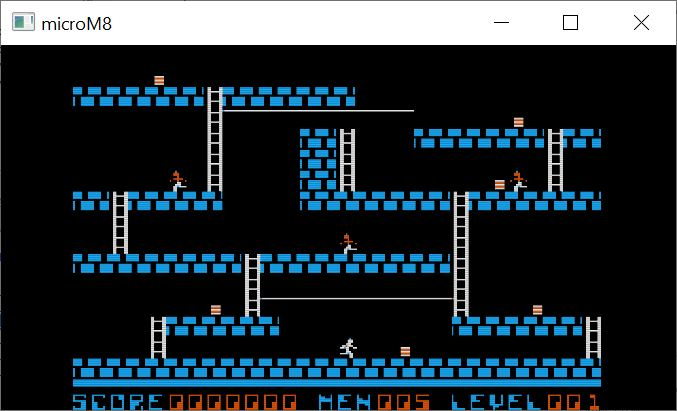
\includegraphics[width=\columnwidth]{screen}
\end{center}

There's a routine to add a 4-digit BCD
number to the score and then update it on the screen.

\nwenddocs{}\nwbegincode{72}\sublabel{NW1Xx3lK-8jv1b-H}\nwmargintag{{\nwtagstyle{}\subpageref{NW1Xx3lK-8jv1b-H}}}\moddef{routines~{\nwtagstyle{}\subpageref{NW1Xx3lK-8jv1b-1}}}\plusendmoddef\nwstartdeflinemarkup\nwusesondefline{\\{NW1Xx3lK-1p0Y9w-1}}\nwprevnextdefs{NW1Xx3lK-8jv1b-G}{NW1Xx3lK-8jv1b-I}\nwenddeflinemarkup
    ORG     $7A92
\nwlinkedidentc{ADD_AND_UPDATE_SCORE}{NW1Xx3lK-8jv1b-H}:
    SUBROUTINE
    ; Enter routine with A set to BCD tens/units and
    ; Y set to BCD thousands/hundreds.

    CLC
    SED                         ; Turn on BCD addition mode.
    ADC     \nwlinkedidentc{SCORE}{NW1Xx3lK-10jlgu-9}
    STA     \nwlinkedidentc{SCORE}{NW1Xx3lK-10jlgu-9}
    TYA
    ADC     \nwlinkedidentc{SCORE}{NW1Xx3lK-10jlgu-9}+1
    STA     \nwlinkedidentc{SCORE}{NW1Xx3lK-10jlgu-9}+1
    LDA     #$00
    ADC     \nwlinkedidentc{SCORE}{NW1Xx3lK-10jlgu-9}+2
    STA     \nwlinkedidentc{SCORE}{NW1Xx3lK-10jlgu-9}+2
    LDA     #$00
    ADC     \nwlinkedidentc{SCORE}{NW1Xx3lK-10jlgu-9}+3
    STA     \nwlinkedidentc{SCORE}{NW1Xx3lK-10jlgu-9}+3             ; \nwlinkedidentc{SCORE}{NW1Xx3lK-10jlgu-9} += param
    CLD                         ; Turn off BCD addition mode.

    LDA     5
    STA     \nwlinkedidentc{GAME_COLNUM}{NW1Xx3lK-10jlgu-5}
    LDA     16
    STA     \nwlinkedidentc{GAME_ROWNUM}{NW1Xx3lK-10jlgu-5}

    LDA     \nwlinkedidentc{SCORE}{NW1Xx3lK-10jlgu-9}+3
    JSR     \nwlinkedidentc{BCD_TO_DECIMAL2}{NW1Xx3lK-8jv1b-G}
    LDA     \nwlinkedidentc{UNITS}{NW1Xx3lK-10jlgu-8}               ; Note we skipped \nwlinkedidentc{TENS}{NW1Xx3lK-10jlgu-8}.
    JSR     \nwlinkedidentc{PUT_DIGIT}{NW1Xx3lK-8jv1b-E}

    LDA     \nwlinkedidentc{SCORE}{NW1Xx3lK-10jlgu-9}+2
    JSR     \nwlinkedidentc{BCD_TO_DECIMAL2}{NW1Xx3lK-8jv1b-G}
    LDA     \nwlinkedidentc{TENS}{NW1Xx3lK-10jlgu-8}
    JSR     \nwlinkedidentc{PUT_DIGIT}{NW1Xx3lK-8jv1b-E}
    LDA     \nwlinkedidentc{UNITS}{NW1Xx3lK-10jlgu-8}
    JSR     \nwlinkedidentc{PUT_DIGIT}{NW1Xx3lK-8jv1b-E}

    LDA     \nwlinkedidentc{SCORE}{NW1Xx3lK-10jlgu-9}+1
    JSR     \nwlinkedidentc{BCD_TO_DECIMAL2}{NW1Xx3lK-8jv1b-G}
    LDA     \nwlinkedidentc{TENS}{NW1Xx3lK-10jlgu-8}
    JSR     \nwlinkedidentc{PUT_DIGIT}{NW1Xx3lK-8jv1b-E}
    LDA     \nwlinkedidentc{UNITS}{NW1Xx3lK-10jlgu-8}
    JSR     \nwlinkedidentc{PUT_DIGIT}{NW1Xx3lK-8jv1b-E}

    LDA     \nwlinkedidentc{SCORE}{NW1Xx3lK-10jlgu-9}
    JSR     \nwlinkedidentc{BCD_TO_DECIMAL2}{NW1Xx3lK-8jv1b-G}
    LDA     \nwlinkedidentc{TENS}{NW1Xx3lK-10jlgu-8}
    JSR     \nwlinkedidentc{PUT_DIGIT}{NW1Xx3lK-8jv1b-E}
    LDA     \nwlinkedidentc{UNITS}{NW1Xx3lK-10jlgu-8}
    JMP     \nwlinkedidentc{PUT_DIGIT}{NW1Xx3lK-8jv1b-E}           ; tail call

\nwindexdefn{\nwixident{ADD{\_}AND{\_}UPDATE{\_}SCORE}}{ADD:unAND:unUPDATE:unSCORE}{NW1Xx3lK-8jv1b-H}\eatline
\nwused{\\{NW1Xx3lK-1p0Y9w-1}}\nwidentdefs{\\{{\nwixident{ADD{\_}AND{\_}UPDATE{\_}SCORE}}{ADD:unAND:unUPDATE:unSCORE}}}\nwidentuses{\\{{\nwixident{BCD{\_}TO{\_}DECIMAL2}}{BCD:unTO:unDECIMAL2}}\\{{\nwixident{GAME{\_}COLNUM}}{GAME:unCOLNUM}}\\{{\nwixident{GAME{\_}ROWNUM}}{GAME:unROWNUM}}\\{{\nwixident{PUT{\_}DIGIT}}{PUT:unDIGIT}}\\{{\nwixident{SCORE}}{SCORE}}\\{{\nwixident{TENS}}{TENS}}\\{{\nwixident{UNITS}}{UNITS}}}\nwindexuse{\nwixident{BCD{\_}TO{\_}DECIMAL2}}{BCD:unTO:unDECIMAL2}{NW1Xx3lK-8jv1b-H}\nwindexuse{\nwixident{GAME{\_}COLNUM}}{GAME:unCOLNUM}{NW1Xx3lK-8jv1b-H}\nwindexuse{\nwixident{GAME{\_}ROWNUM}}{GAME:unROWNUM}{NW1Xx3lK-8jv1b-H}\nwindexuse{\nwixident{PUT{\_}DIGIT}}{PUT:unDIGIT}{NW1Xx3lK-8jv1b-H}\nwindexuse{\nwixident{SCORE}}{SCORE}{NW1Xx3lK-8jv1b-H}\nwindexuse{\nwixident{TENS}}{TENS}{NW1Xx3lK-8jv1b-H}\nwindexuse{\nwixident{UNITS}}{UNITS}{NW1Xx3lK-8jv1b-H}\nwendcode{}\nwbegindocs{73}\nwdocspar
The other elements in the status line are the number of men
(i.e. lives) and the current level.

\nwenddocs{}\nwbegincode{74}\sublabel{NW1Xx3lK-10jlgu-A}\nwmargintag{{\nwtagstyle{}\subpageref{NW1Xx3lK-10jlgu-A}}}\moddef{defines~{\nwtagstyle{}\subpageref{NW1Xx3lK-10jlgu-1}}}\plusendmoddef\nwstartdeflinemarkup\nwusesondefline{\\{NW1Xx3lK-1p0Y9w-1}}\nwprevnextdefs{NW1Xx3lK-10jlgu-9}{NW1Xx3lK-10jlgu-B}\nwenddeflinemarkup
    ORG     $A6
\nwlinkedidentc{LEVELNUM}{NW1Xx3lK-10jlgu-A}    DS      1
    ORG     $C8
\nwlinkedidentc{LIVES}{NW1Xx3lK-10jlgu-A}       DS      1
\nwindexdefn{\nwixident{LEVELNUM}}{LEVELNUM}{NW1Xx3lK-10jlgu-A}\nwindexdefn{\nwixident{LIVES}}{LIVES}{NW1Xx3lK-10jlgu-A}\eatline
\nwused{\\{NW1Xx3lK-1p0Y9w-1}}\nwidentdefs{\\{{\nwixident{LEVELNUM}}{LEVELNUM}}\\{{\nwixident{LIVES}}{LIVES}}}\nwendcode{}\nwbegindocs{75}\nwdocspar
Here are the routines to put the lives and level number on
the status line. Lives starts at column 16, and level number
starts at column 25.

\nwenddocs{}\nwbegincode{76}\sublabel{NW1Xx3lK-8jv1b-I}\nwmargintag{{\nwtagstyle{}\subpageref{NW1Xx3lK-8jv1b-I}}}\moddef{routines~{\nwtagstyle{}\subpageref{NW1Xx3lK-8jv1b-1}}}\plusendmoddef\nwstartdeflinemarkup\nwusesondefline{\\{NW1Xx3lK-1p0Y9w-1}}\nwprevnextdefs{NW1Xx3lK-8jv1b-H}{NW1Xx3lK-8jv1b-J}\nwenddeflinemarkup
    ORG     $7a70
\nwlinkedidentc{PUT_STATUS_LIVES}{NW1Xx3lK-8jv1b-I}:
    SUBROUTINE

    LDA     \nwlinkedidentc{LIVES}{NW1Xx3lK-10jlgu-A}
    LDX     16
    ; fallthrough

PUT_STATUS_BYTE:
    SUBROUTINE
    ; Puts the number in A as a three-digit decimal on the screen
    ; at row 16, column X.

    STX     \nwlinkedidentc{GAME_COLNUM}{NW1Xx3lK-10jlgu-5}
    JSR     \nwlinkedidentc{TO_DECIMAL3}{NW1Xx3lK-8jv1b-F}
    LDA     16
    STA     \nwlinkedidentc{GAME_ROWNUM}{NW1Xx3lK-10jlgu-5}
    LDA     \nwlinkedidentc{HUNDREDS}{NW1Xx3lK-10jlgu-8}
    JSR     \nwlinkedidentc{PUT_DIGIT}{NW1Xx3lK-8jv1b-E}
    LDA     \nwlinkedidentc{TENS}{NW1Xx3lK-10jlgu-8}
    JSR     \nwlinkedidentc{PUT_DIGIT}{NW1Xx3lK-8jv1b-E}
    LDA     \nwlinkedidentc{UNITS}{NW1Xx3lK-10jlgu-8}
    JMP     \nwlinkedidentc{PUT_DIGIT}{NW1Xx3lK-8jv1b-E}           ; tail call

\nwlinkedidentc{PUT_STATUS_LEVEL}{NW1Xx3lK-8jv1b-I}:
    SUBROUTINE

    LDA     \nwlinkedidentc{LEVELNUM}{NW1Xx3lK-10jlgu-A}
    LDX     25
    BNE     PUT_STATUS_BYTE     ; Unconditional jump

\nwindexdefn{\nwixident{PUT{\_}STATUS{\_}LIVES}}{PUT:unSTATUS:unLIVES}{NW1Xx3lK-8jv1b-I}\nwindexdefn{\nwixident{PUT{\_}STATUS{\_}LEVEL}}{PUT:unSTATUS:unLEVEL}{NW1Xx3lK-8jv1b-I}\eatline
\nwused{\\{NW1Xx3lK-1p0Y9w-1}}\nwidentdefs{\\{{\nwixident{PUT{\_}STATUS{\_}LEVEL}}{PUT:unSTATUS:unLEVEL}}\\{{\nwixident{PUT{\_}STATUS{\_}LIVES}}{PUT:unSTATUS:unLIVES}}}\nwidentuses{\\{{\nwixident{GAME{\_}COLNUM}}{GAME:unCOLNUM}}\\{{\nwixident{GAME{\_}ROWNUM}}{GAME:unROWNUM}}\\{{\nwixident{HUNDREDS}}{HUNDREDS}}\\{{\nwixident{LEVELNUM}}{LEVELNUM}}\\{{\nwixident{LIVES}}{LIVES}}\\{{\nwixident{PUT{\_}DIGIT}}{PUT:unDIGIT}}\\{{\nwixident{TENS}}{TENS}}\\{{\nwixident{TO{\_}DECIMAL3}}{TO:unDECIMAL3}}\\{{\nwixident{UNITS}}{UNITS}}}\nwindexuse{\nwixident{GAME{\_}COLNUM}}{GAME:unCOLNUM}{NW1Xx3lK-8jv1b-I}\nwindexuse{\nwixident{GAME{\_}ROWNUM}}{GAME:unROWNUM}{NW1Xx3lK-8jv1b-I}\nwindexuse{\nwixident{HUNDREDS}}{HUNDREDS}{NW1Xx3lK-8jv1b-I}\nwindexuse{\nwixident{LEVELNUM}}{LEVELNUM}{NW1Xx3lK-8jv1b-I}\nwindexuse{\nwixident{LIVES}}{LIVES}{NW1Xx3lK-8jv1b-I}\nwindexuse{\nwixident{PUT{\_}DIGIT}}{PUT:unDIGIT}{NW1Xx3lK-8jv1b-I}\nwindexuse{\nwixident{TENS}}{TENS}{NW1Xx3lK-8jv1b-I}\nwindexuse{\nwixident{TO{\_}DECIMAL3}}{TO:unDECIMAL3}{NW1Xx3lK-8jv1b-I}\nwindexuse{\nwixident{UNITS}}{UNITS}{NW1Xx3lK-8jv1b-I}\nwendcode{}\nwbegindocs{77}\nwdocspar
\chapter{Sound}

\section{Sound "strings"}

A sound "string" describes a sound to play in terms of pitch and duration, ending in a {\Tt{}00\nwendquote}.
Just like in the {\Tt{}\nwlinkedidentq{PUT{\_}STRING}{NW1Xx3lK-8jv1b-D}\nwendquote} routine, rather than take
an address pointing to a sound string, instead it uses the return address as the source for data.
It then has to fix up the actual return address at the end to be just after the zero-terminating
byte of the string.

Because {\Tt{}\nwlinkedidentq{NOTE{\_}INDEX}{NW1Xx3lK-10jlgu-B}\nwendquote} is not zeroed out, this actually appends to the sound data buffer.

The format of a sound string is duration, followed by pitch, although the pitch is lower for higher numbers.

One example of a sound string is {\Tt{}07\ 45\ 06\ 55\ 05\ 44\ 04\ 54\ 03\ 43\ 02\ 53\nwendquote}, found in {\Tt{}CHECK{\_}FOR{\_}GOLD{\_}PICKED{\_}UP{\_}BY{\_}PLAYER\nwendquote}.


\nwenddocs{}\nwbegincode{78}\sublabel{NW1Xx3lK-10jlgu-B}\nwmargintag{{\nwtagstyle{}\subpageref{NW1Xx3lK-10jlgu-B}}}\moddef{defines~{\nwtagstyle{}\subpageref{NW1Xx3lK-10jlgu-1}}}\plusendmoddef\nwstartdeflinemarkup\nwusesondefline{\\{NW1Xx3lK-1p0Y9w-1}}\nwprevnextdefs{NW1Xx3lK-10jlgu-A}{NW1Xx3lK-10jlgu-C}\nwenddeflinemarkup
\nwlinkedidentc{NOTE_INDEX}{NW1Xx3lK-10jlgu-B}      EQU     $54
\nwlinkedidentc{SOUND_DURATION}{NW1Xx3lK-10jlgu-B}  EQU     $0E00       ; 128 bytes
\nwlinkedidentc{SOUND_PITCH}{NW1Xx3lK-10jlgu-B}     EQU     $0E80       ; 128 bytes
\nwindexdefn{\nwixident{NOTE{\_}INDEX}}{NOTE:unINDEX}{NW1Xx3lK-10jlgu-B}\nwindexdefn{\nwixident{SOUND{\_}DURATION}}{SOUND:unDURATION}{NW1Xx3lK-10jlgu-B}\nwindexdefn{\nwixident{SOUND{\_}PITCH}}{SOUND:unPITCH}{NW1Xx3lK-10jlgu-B}\eatline
\nwused{\\{NW1Xx3lK-1p0Y9w-1}}\nwidentdefs{\\{{\nwixident{NOTE{\_}INDEX}}{NOTE:unINDEX}}\\{{\nwixident{SOUND{\_}DURATION}}{SOUND:unDURATION}}\\{{\nwixident{SOUND{\_}PITCH}}{SOUND:unPITCH}}}\nwendcode{}\nwbegindocs{79}\nwdocspar
\nwenddocs{}\nwbegincode{80}\sublabel{NW1Xx3lK-90gdY-1}\nwmargintag{{\nwtagstyle{}\subpageref{NW1Xx3lK-90gdY-1}}}\moddef{load sound data~{\nwtagstyle{}\subpageref{NW1Xx3lK-90gdY-1}}}\endmoddef\nwstartdeflinemarkup\nwusesondefline{\\{NW1Xx3lK-8jv1b-K}}\nwenddeflinemarkup
    ORG     $87E1
\nwlinkedidentc{LOAD_SOUND_DATA}{NW1Xx3lK-90gdY-1}:
    SUBROUTINE

    PLA
    STA     \nwlinkedidentc{SAVED_RET_ADDR}{NW1Xx3lK-10jlgu-7}
    PLA
    STA     \nwlinkedidentc{SAVED_RET_ADDR}{NW1Xx3lK-10jlgu-7}+1
    BNE     .next

.loop:
    LDY     #$00
    LDA     (\nwlinkedidentc{SAVED_RET_ADDR}{NW1Xx3lK-10jlgu-7}),Y
    BEQ     .end
    INC     \nwlinkedidentc{NOTE_INDEX}{NW1Xx3lK-10jlgu-B}
    LDX     \nwlinkedidentc{NOTE_INDEX}{NW1Xx3lK-10jlgu-B}
    STA     \nwlinkedidentc{SOUND_DURATION}{NW1Xx3lK-10jlgu-B},X
    INY
    LDA     (\nwlinkedidentc{SAVED_RET_ADDR}{NW1Xx3lK-10jlgu-7}),Y
    STA     \nwlinkedidentc{SOUND_PITCH}{NW1Xx3lK-10jlgu-B},X

    INC     \nwlinkedidentc{SAVED_RET_ADDR}{NW1Xx3lK-10jlgu-7}
    BNE     .next
    INC     \nwlinkedidentc{SAVED_RET_ADDR}{NW1Xx3lK-10jlgu-7}+1

.next:
    INC     \nwlinkedidentc{SAVED_RET_ADDR}{NW1Xx3lK-10jlgu-7}
    BNE     .loop
    INC     \nwlinkedidentc{SAVED_RET_ADDR}{NW1Xx3lK-10jlgu-7}+1
    BNE     .loop

.end:
    LDA     \nwlinkedidentc{SAVED_RET_ADDR}{NW1Xx3lK-10jlgu-7}+1
    PHA
    LDA     \nwlinkedidentc{SAVED_RET_ADDR}{NW1Xx3lK-10jlgu-7}
    PHA
    RTS
\nwindexdefn{\nwixident{LOAD{\_}SOUND{\_}DATA}}{LOAD:unSOUND:unDATA}{NW1Xx3lK-90gdY-1}\eatline
\nwused{\\{NW1Xx3lK-8jv1b-K}}\nwidentdefs{\\{{\nwixident{LOAD{\_}SOUND{\_}DATA}}{LOAD:unSOUND:unDATA}}}\nwidentuses{\\{{\nwixident{NOTE{\_}INDEX}}{NOTE:unINDEX}}\\{{\nwixident{SAVED{\_}RET{\_}ADDR}}{SAVED:unRET:unADDR}}\\{{\nwixident{SOUND{\_}DURATION}}{SOUND:unDURATION}}\\{{\nwixident{SOUND{\_}PITCH}}{SOUND:unPITCH}}}\nwindexuse{\nwixident{NOTE{\_}INDEX}}{NOTE:unINDEX}{NW1Xx3lK-90gdY-1}\nwindexuse{\nwixident{SAVED{\_}RET{\_}ADDR}}{SAVED:unRET:unADDR}{NW1Xx3lK-90gdY-1}\nwindexuse{\nwixident{SOUND{\_}DURATION}}{SOUND:unDURATION}{NW1Xx3lK-90gdY-1}\nwindexuse{\nwixident{SOUND{\_}PITCH}}{SOUND:unPITCH}{NW1Xx3lK-90gdY-1}\nwendcode{}\nwbegindocs{81}\nwdocspar
\section{Playing notes}

The {\Tt{}\nwlinkedidentq{PLAY{\_}NOTE}{NW1Xx3lK-1Ew0EG-1}\nwendquote} routines plays a note through the built-in speaker. The time the note is played is
based on X and Y forming a 16-bit counter (X being the most significant byte), but A controls the pitch,
which is how often the speaker is clicked. The higher A, the lower the pitch.

The {\Tt{}\nwlinkedidentq{ENABLE{\_}SOUND}{NW1Xx3lK-10jlgu-C}\nwendquote} location can also disable playing the note, but the routine still takes as long as it would have.

\nwenddocs{}\nwbegincode{82}\sublabel{NW1Xx3lK-10jlgu-C}\nwmargintag{{\nwtagstyle{}\subpageref{NW1Xx3lK-10jlgu-C}}}\moddef{defines~{\nwtagstyle{}\subpageref{NW1Xx3lK-10jlgu-1}}}\plusendmoddef\nwstartdeflinemarkup\nwusesondefline{\\{NW1Xx3lK-1p0Y9w-1}}\nwprevnextdefs{NW1Xx3lK-10jlgu-B}{NW1Xx3lK-10jlgu-D}\nwenddeflinemarkup
\nwlinkedidentc{ENABLE_SOUND}{NW1Xx3lK-10jlgu-C}    EQU     $99     ; If 0, do not click speaker.
\nwlinkedidentc{SPKR}{NW1Xx3lK-10jlgu-C}            EQU     $C030   ; Access clicks the speaker.
\nwindexdefn{\nwixident{ENABLE{\_}SOUND}}{ENABLE:unSOUND}{NW1Xx3lK-10jlgu-C}\nwindexdefn{\nwixident{SPKR}}{SPKR}{NW1Xx3lK-10jlgu-C}\eatline
\nwused{\\{NW1Xx3lK-1p0Y9w-1}}\nwidentdefs{\\{{\nwixident{ENABLE{\_}SOUND}}{ENABLE:unSOUND}}\\{{\nwixident{SPKR}}{SPKR}}}\nwendcode{}\nwbegindocs{83}\nwdocspar
\nwenddocs{}\nwbegincode{84}\sublabel{NW1Xx3lK-1Ew0EG-1}\nwmargintag{{\nwtagstyle{}\subpageref{NW1Xx3lK-1Ew0EG-1}}}\moddef{play note~{\nwtagstyle{}\subpageref{NW1Xx3lK-1Ew0EG-1}}}\endmoddef\nwstartdeflinemarkup\nwusesondefline{\\{NW1Xx3lK-8jv1b-K}}\nwenddeflinemarkup
    ORG     $87BA
\nwlinkedidentc{PLAY_NOTE}{NW1Xx3lK-1Ew0EG-1}:
    SUBROUTINE

    STA     \nwlinkedidentc{TMP_PTR}{NW1Xx3lK-10jlgu-1}
    STX     \nwlinkedidentc{TMP_PTR}{NW1Xx3lK-10jlgu-1}+1

.loop:
    LDA     \nwlinkedidentc{ENABLE_SOUND}{NW1Xx3lK-10jlgu-C}
    BEQ     .decrement_counter
    LDA     \nwlinkedidentc{SPKR}{NW1Xx3lK-10jlgu-C}

.decrement_counter:
    DEY
    BNE     .counter_decremented
    DEC     \nwlinkedidentc{TMP_PTR}{NW1Xx3lK-10jlgu-1}+1
    BEQ     .end

.counter_decremented:
    DEX
    BNE     .decrement_counter
    LDX     \nwlinkedidentc{TMP_PTR}{NW1Xx3lK-10jlgu-1}
    JMP     .loop

.end:
    RTS
\nwindexdefn{\nwixident{PLAY{\_}NOTE}}{PLAY:unNOTE}{NW1Xx3lK-1Ew0EG-1}\eatline
\nwused{\\{NW1Xx3lK-8jv1b-K}}\nwidentdefs{\\{{\nwixident{PLAY{\_}NOTE}}{PLAY:unNOTE}}}\nwidentuses{\\{{\nwixident{ENABLE{\_}SOUND}}{ENABLE:unSOUND}}\\{{\nwixident{SPKR}}{SPKR}}\\{{\nwixident{TMP{\_}PTR}}{TMP:unPTR}}}\nwindexuse{\nwixident{ENABLE{\_}SOUND}}{ENABLE:unSOUND}{NW1Xx3lK-1Ew0EG-1}\nwindexuse{\nwixident{SPKR}}{SPKR}{NW1Xx3lK-1Ew0EG-1}\nwindexuse{\nwixident{TMP{\_}PTR}}{TMP:unPTR}{NW1Xx3lK-1Ew0EG-1}\nwendcode{}\nwbegindocs{85}\nwdocspar
\section{Playing a sound}

The {\Tt{}\nwlinkedidentq{SOUND{\_}DELAY}{NW1Xx3lK-3j1fAh-1}\nwendquote} routine delays an amount of time based on the X register. The total number of cycles is about 905 per each X.
Since the Apple //e clock cycle was 980 nsec (on an NTSC system), this routine would delay approximately 887 microseconds times X.
PAL systems were very slightly slower (by $0.47\%$), which corresponds to 883 microseconds times X.

\nwenddocs{}\nwbegincode{86}\sublabel{NW1Xx3lK-3j1fAh-1}\nwmargintag{{\nwtagstyle{}\subpageref{NW1Xx3lK-3j1fAh-1}}}\moddef{sound delay~{\nwtagstyle{}\subpageref{NW1Xx3lK-3j1fAh-1}}}\endmoddef\nwstartdeflinemarkup\nwusesondefline{\\{NW1Xx3lK-8jv1b-K}}\nwenddeflinemarkup
    ORG     $86B5
\nwlinkedidentc{SOUND_DELAY}{NW1Xx3lK-3j1fAh-1}:
    SUBROUTINE

    LDY     #$B4        ; 180
.loop:
    DEY                 ; 2 cycles
    BNE     .loop       ; 3 cycles
    DEX                 ; 2 cycles
    BNE     .loop       ; 3 cycles
    RTS
\nwindexdefn{\nwixident{SOUND{\_}DELAY}}{SOUND:unDELAY}{NW1Xx3lK-3j1fAh-1}\eatline
\nwused{\\{NW1Xx3lK-8jv1b-K}}\nwidentdefs{\\{{\nwixident{SOUND{\_}DELAY}}{SOUND:unDELAY}}}\nwendcode{}\nwbegindocs{87}\nwdocspar
Finally, the {\Tt{}\nwlinkedidentq{PLAY{\_}SOUND}{NW1Xx3lK-4DEk44-1}\nwendquote} routine plays one section of the sound string stored in the {\Tt{}\nwlinkedidentq{SOUND{\_}PITCH}{NW1Xx3lK-10jlgu-B}\nwendquote}
and {\Tt{}\nwlinkedidentq{SOUND{\_}DURATION}{NW1Xx3lK-10jlgu-B}\nwendquote} buffers. We have to break up the playing of the sound so that gameplay doesn't
pause while playing the sound, although game play does pause while playing the note.

Alternatively, if there is no sound string, we can play the note stored in location {\Tt{}{\nwbackslash}{\$}A4\nwendquote} as long as
location {\Tt{}{\nwbackslash}{\$}9B\nwendquote} is zero. The duration is {\Tt{}2\ +\ \nwlinkedidentq{SOUND{\_}PERIOD}{NW1Xx3lK-10jlgu-D}\nwendquote}.

The routine is designed to delay approximately the same amount regardless of sound duration. The
delay is controlled by {\Tt{}\nwlinkedidentq{SOUND{\_}PERIOD}{NW1Xx3lK-10jlgu-D}\nwendquote}. This value is hardcoded to {\Tt{}6\nwendquote}.

\nwenddocs{}\nwbegincode{88}\sublabel{NW1Xx3lK-10jlgu-D}\nwmargintag{{\nwtagstyle{}\subpageref{NW1Xx3lK-10jlgu-D}}}\moddef{defines~{\nwtagstyle{}\subpageref{NW1Xx3lK-10jlgu-1}}}\plusendmoddef\nwstartdeflinemarkup\nwusesondefline{\\{NW1Xx3lK-1p0Y9w-1}}\nwprevnextdefs{NW1Xx3lK-10jlgu-C}{NW1Xx3lK-10jlgu-E}\nwenddeflinemarkup
    ORG     $8C
\nwlinkedidentc{SOUND_PERIOD}{NW1Xx3lK-10jlgu-D}:
    HEX     06
\nwindexdefn{\nwixident{SOUND{\_}PERIOD}}{SOUND:unPERIOD}{NW1Xx3lK-10jlgu-D}\eatline
\nwused{\\{NW1Xx3lK-1p0Y9w-1}}\nwidentdefs{\\{{\nwixident{SOUND{\_}PERIOD}}{SOUND:unPERIOD}}}\nwendcode{}\nwbegindocs{89}\nwdocspar
\nwenddocs{}\nwbegincode{90}\sublabel{NW1Xx3lK-4DEk44-1}\nwmargintag{{\nwtagstyle{}\subpageref{NW1Xx3lK-4DEk44-1}}}\moddef{play sound~{\nwtagstyle{}\subpageref{NW1Xx3lK-4DEk44-1}}}\endmoddef\nwstartdeflinemarkup\nwusesondefline{\\{NW1Xx3lK-8jv1b-K}}\nwenddeflinemarkup
    ORG     $8811
\nwlinkedidentc{PLAY_SOUND}{NW1Xx3lK-4DEk44-1}:
    SUBROUTINE

    LDY     \nwlinkedidentc{NOTE_INDEX}{NW1Xx3lK-10jlgu-B}
    BEQ     .no_more_notes
    LDA     \nwlinkedidentc{SOUND_PITCH}{NW1Xx3lK-10jlgu-B},Y
    LDX     \nwlinkedidentc{SOUND_DURATION}{NW1Xx3lK-10jlgu-B},Y
    JSR     \nwlinkedidentc{PLAY_NOTE}{NW1Xx3lK-1Ew0EG-1}

    LDY     \nwlinkedidentc{NOTE_INDEX}{NW1Xx3lK-10jlgu-B}              ; Y = \nwlinkedidentc{NOTE_INDEX}{NW1Xx3lK-10jlgu-B}
    DEC     \nwlinkedidentc{NOTE_INDEX}{NW1Xx3lK-10jlgu-B}              ; \nwlinkedidentc{NOTE_INDEX}{NW1Xx3lK-10jlgu-B}--
    LDA     \nwlinkedidentc{SOUND_PERIOD}{NW1Xx3lK-10jlgu-D}
    SEC
    SBC     \nwlinkedidentc{SOUND_DURATION}{NW1Xx3lK-10jlgu-B},Y        ; A = \nwlinkedidentc{SOUND_PERIOD}{NW1Xx3lK-10jlgu-D} - \nwlinkedidentc{SOUND_DURATION}{NW1Xx3lK-10jlgu-B}[Y]
    BEQ     .done
    BCC     .done                   ; If A <= 0, done.
    TAX
    JSR     \nwlinkedidentc{SOUND_DELAY}{NW1Xx3lK-3j1fAh-1}

.done:
    SEC
    RTS

.no_more_notes:
    LDA     $9B
    BNE     .end
    LDA     $A4
    LSR                     ; pitch = $A4 >> 1
    INC     $A4             ; $A4++
    LDX     \nwlinkedidentc{SOUND_PERIOD}{NW1Xx3lK-10jlgu-D}
    INX
    INX                     ; duration = \nwlinkedidentc{SOUND_PERIOD}{NW1Xx3lK-10jlgu-D} + 2
    JSR     \nwlinkedidentc{PLAY_NOTE}{NW1Xx3lK-1Ew0EG-1}

    CLC
    RTS

.end:
    LDX     \nwlinkedidentc{SOUND_PERIOD}{NW1Xx3lK-10jlgu-D}
    JSR     \nwlinkedidentc{SOUND_DELAY}{NW1Xx3lK-3j1fAh-1}

    CLC
    RTS
\nwindexdefn{\nwixident{PLAY{\_}SOUND}}{PLAY:unSOUND}{NW1Xx3lK-4DEk44-1}\eatline
\nwused{\\{NW1Xx3lK-8jv1b-K}}\nwidentdefs{\\{{\nwixident{PLAY{\_}SOUND}}{PLAY:unSOUND}}}\nwidentuses{\\{{\nwixident{NOTE{\_}INDEX}}{NOTE:unINDEX}}\\{{\nwixident{PLAY{\_}NOTE}}{PLAY:unNOTE}}\\{{\nwixident{SOUND{\_}DELAY}}{SOUND:unDELAY}}\\{{\nwixident{SOUND{\_}DURATION}}{SOUND:unDURATION}}\\{{\nwixident{SOUND{\_}PERIOD}}{SOUND:unPERIOD}}\\{{\nwixident{SOUND{\_}PITCH}}{SOUND:unPITCH}}}\nwindexuse{\nwixident{NOTE{\_}INDEX}}{NOTE:unINDEX}{NW1Xx3lK-4DEk44-1}\nwindexuse{\nwixident{PLAY{\_}NOTE}}{PLAY:unNOTE}{NW1Xx3lK-4DEk44-1}\nwindexuse{\nwixident{SOUND{\_}DELAY}}{SOUND:unDELAY}{NW1Xx3lK-4DEk44-1}\nwindexuse{\nwixident{SOUND{\_}DURATION}}{SOUND:unDURATION}{NW1Xx3lK-4DEk44-1}\nwindexuse{\nwixident{SOUND{\_}PERIOD}}{SOUND:unPERIOD}{NW1Xx3lK-4DEk44-1}\nwindexuse{\nwixident{SOUND{\_}PITCH}}{SOUND:unPITCH}{NW1Xx3lK-4DEk44-1}\nwendcode{}\nwbegindocs{91}\nwdocspar
\chapter{Levels}

One of the appealing things about Lode Runner are its levels. 150 levels are stored
in the game, and there is even a level editor included.

\section{Drawing a level}

Let's see how Lode Runner draws a level. We start with the routine {\Tt{}\nwlinkedidentq{DRAW{\_}LEVEL{\_}PAGE2}{NW1Xx3lK-2Mcso2-1}\nwendquote},
which draws a level on HGR2. Note that HGR1 would be displayed, so the player doesn't
see the draw happening.

We start by looping backwards over rows 15 through 0:

\nwenddocs{}\nwbegincode{92}\sublabel{NW1Xx3lK-2Mcso2-1}\nwmargintag{{\nwtagstyle{}\subpageref{NW1Xx3lK-2Mcso2-1}}}\moddef{level draw routine~{\nwtagstyle{}\subpageref{NW1Xx3lK-2Mcso2-1}}}\endmoddef\nwstartdeflinemarkup\nwusesondefline{\\{NW1Xx3lK-8jv1b-K}}\nwprevnextdefs{\relax}{NW1Xx3lK-2Mcso2-2}\nwenddeflinemarkup
    ORG     $63B3
\nwlinkedidentc{DRAW_LEVEL_PAGE2}{NW1Xx3lK-2Mcso2-1}:
    SUBROUTINE
    ; Returns carry set if there was no player sprite in the level,
    ; or carry clear if there was.

    LDY     15
    STY     \nwlinkedidentc{GAME_ROWNUM}{NW1Xx3lK-10jlgu-5}

.row_loop:
\nwindexdefn{\nwixident{DRAW{\_}LEVEL{\_}PAGE2}}{DRAW:unLEVEL:unPAGE2}{NW1Xx3lK-2Mcso2-1}\eatline
\nwalsodefined{\\{NW1Xx3lK-2Mcso2-2}\\{NW1Xx3lK-2Mcso2-3}\\{NW1Xx3lK-2Mcso2-4}\\{NW1Xx3lK-2Mcso2-5}\\{NW1Xx3lK-2Mcso2-6}\\{NW1Xx3lK-2Mcso2-7}\\{NW1Xx3lK-2Mcso2-8}\\{NW1Xx3lK-2Mcso2-9}\\{NW1Xx3lK-2Mcso2-A}\\{NW1Xx3lK-2Mcso2-B}\\{NW1Xx3lK-2Mcso2-C}\\{NW1Xx3lK-2Mcso2-D}\\{NW1Xx3lK-2Mcso2-E}\\{NW1Xx3lK-2Mcso2-F}\\{NW1Xx3lK-2Mcso2-G}}\nwused{\\{NW1Xx3lK-8jv1b-K}}\nwidentdefs{\\{{\nwixident{DRAW{\_}LEVEL{\_}PAGE2}}{DRAW:unLEVEL:unPAGE2}}}\nwidentuses{\\{{\nwixident{GAME{\_}ROWNUM}}{GAME:unROWNUM}}}\nwindexuse{\nwixident{GAME{\_}ROWNUM}}{GAME:unROWNUM}{NW1Xx3lK-2Mcso2-1}\nwendcode{}\nwbegindocs{93}\nwdocspar
We'll assume the level data is stored in
a table which contains 16 pointers, one for each row. As usual in Lode Runner,
the pages and offsets for those pointers are stored in separate tables. these
are {\Tt{}\nwlinkedidentq{CURR{\_}LEVEL{\_}ROW{\_}SPRITES{\_}PTR{\_}PAGES}{NW1Xx3lK-1W8AJS-A}\nwendquote} and {\Tt{}\nwlinkedidentq{CURR{\_}LEVEL{\_}ROW{\_}SPRITES{\_}PTR{\_}OFFSETS}{NW1Xx3lK-1W8AJS-A}\nwendquote}.

\nwenddocs{}\nwbegincode{94}\sublabel{NW1Xx3lK-1W8AJS-A}\nwmargintag{{\nwtagstyle{}\subpageref{NW1Xx3lK-1W8AJS-A}}}\moddef{tables~{\nwtagstyle{}\subpageref{NW1Xx3lK-1W8AJS-1}}}\plusendmoddef\nwstartdeflinemarkup\nwusesondefline{\\{NW1Xx3lK-1p0Y9w-1}}\nwprevnextdefs{NW1Xx3lK-1W8AJS-9}{NW1Xx3lK-1W8AJS-B}\nwenddeflinemarkup
    ORG     $1C05
\nwlinkedidentc{CURR_LEVEL_ROW_SPRITES_PTR_OFFSETS}{NW1Xx3lK-1W8AJS-A}:
    HEX     00 1C 38 54 70 8C A8 C4 E0 FC 18 34 50 6C 88 A4
\nwlinkedidentc{CURR_LEVEL_ROW_SPRITES_PTR_PAGES}{NW1Xx3lK-1W8AJS-A}:
    HEX     08 08 08 08 08 08 08 08 08 08 09 09 09 09 09 09
\nwlinkedidentc{CURR_LEVEL_ROW_SPRITES_PTR_PAGES2}{NW1Xx3lK-1W8AJS-A}:
    HEX     0A 0A 0A 0A 0A 0A 0A 0A 0A 0A 0B 0B 0B 0B 0B 0B
\nwindexdefn{\nwixident{CURR{\_}LEVEL{\_}ROW{\_}SPRITES{\_}PTR{\_}OFFSETS}}{CURR:unLEVEL:unROW:unSPRITES:unPTR:unOFFSETS}{NW1Xx3lK-1W8AJS-A}\nwindexdefn{\nwixident{CURR{\_}LEVEL{\_}ROW{\_}SPRITES{\_}PTR{\_}PAGES}}{CURR:unLEVEL:unROW:unSPRITES:unPTR:unPAGES}{NW1Xx3lK-1W8AJS-A}\nwindexdefn{\nwixident{CURR{\_}LEVEL{\_}ROW{\_}SPRITES{\_}PTR{\_}PAGES2}}{CURR:unLEVEL:unROW:unSPRITES:unPTR:unPAGES2}{NW1Xx3lK-1W8AJS-A}\eatline
\nwused{\\{NW1Xx3lK-1p0Y9w-1}}\nwidentdefs{\\{{\nwixident{CURR{\_}LEVEL{\_}ROW{\_}SPRITES{\_}PTR{\_}OFFSETS}}{CURR:unLEVEL:unROW:unSPRITES:unPTR:unOFFSETS}}\\{{\nwixident{CURR{\_}LEVEL{\_}ROW{\_}SPRITES{\_}PTR{\_}PAGES}}{CURR:unLEVEL:unROW:unSPRITES:unPTR:unPAGES}}\\{{\nwixident{CURR{\_}LEVEL{\_}ROW{\_}SPRITES{\_}PTR{\_}PAGES2}}{CURR:unLEVEL:unROW:unSPRITES:unPTR:unPAGES2}}}\nwendcode{}\nwbegindocs{95}\nwdocspar
At the beginning of this loop, we create two pointers which we'll simply
call {\Tt{}\nwlinkedidentq{PTR1}{NW1Xx3lK-10jlgu-E}\nwendquote} and {\Tt{}\nwlinkedidentq{PTR2}{NW1Xx3lK-10jlgu-E}\nwendquote}. 

\nwenddocs{}\nwbegincode{96}\sublabel{NW1Xx3lK-10jlgu-E}\nwmargintag{{\nwtagstyle{}\subpageref{NW1Xx3lK-10jlgu-E}}}\moddef{defines~{\nwtagstyle{}\subpageref{NW1Xx3lK-10jlgu-1}}}\plusendmoddef\nwstartdeflinemarkup\nwusesondefline{\\{NW1Xx3lK-1p0Y9w-1}}\nwprevnextdefs{NW1Xx3lK-10jlgu-D}{NW1Xx3lK-10jlgu-F}\nwenddeflinemarkup
\nwlinkedidentc{PTR1}{NW1Xx3lK-10jlgu-E}        EQU     $06     ; 2 bytes
\nwlinkedidentc{PTR2}{NW1Xx3lK-10jlgu-E}        EQU     $08     ; 2 bytes
\nwindexdefn{\nwixident{PTR1}}{PTR1}{NW1Xx3lK-10jlgu-E}\nwindexdefn{\nwixident{PTR2}}{PTR2}{NW1Xx3lK-10jlgu-E}\eatline
\nwused{\\{NW1Xx3lK-1p0Y9w-1}}\nwidentdefs{\\{{\nwixident{PTR1}}{PTR1}}\\{{\nwixident{PTR2}}{PTR2}}}\nwendcode{}\nwbegindocs{97}\nwdocspar
We set {\Tt{}\nwlinkedidentq{PTR1}{NW1Xx3lK-10jlgu-E}\nwendquote} to the pointer corresponding to the current row, and {\Tt{}\nwlinkedidentq{PTR2}{NW1Xx3lK-10jlgu-E}\nwendquote} to the other
page, though I don't know what it's for yet.

\nwenddocs{}\nwbegincode{98}\sublabel{NW1Xx3lK-2Mcso2-2}\nwmargintag{{\nwtagstyle{}\subpageref{NW1Xx3lK-2Mcso2-2}}}\moddef{level draw routine~{\nwtagstyle{}\subpageref{NW1Xx3lK-2Mcso2-1}}}\plusendmoddef\nwstartdeflinemarkup\nwusesondefline{\\{NW1Xx3lK-8jv1b-K}}\nwprevnextdefs{NW1Xx3lK-2Mcso2-1}{NW1Xx3lK-2Mcso2-3}\nwenddeflinemarkup
    LDA     \nwlinkedidentc{CURR_LEVEL_ROW_SPRITES_PTR_OFFSETS}{NW1Xx3lK-1W8AJS-A},Y
    STA     \nwlinkedidentc{PTR1}{NW1Xx3lK-10jlgu-E}
    STA     \nwlinkedidentc{PTR2}{NW1Xx3lK-10jlgu-E}
    LDA     \nwlinkedidentc{CURR_LEVEL_ROW_SPRITES_PTR_PAGES}{NW1Xx3lK-1W8AJS-A},Y
    STA     \nwlinkedidentc{PTR1}{NW1Xx3lK-10jlgu-E}+1
    LDA     \nwlinkedidentc{CURR_LEVEL_ROW_SPRITES_PTR_PAGES2}{NW1Xx3lK-1W8AJS-A},Y
    STA     \nwlinkedidentc{PTR2}{NW1Xx3lK-10jlgu-E}+1
\nwused{\\{NW1Xx3lK-8jv1b-K}}\nwidentuses{\\{{\nwixident{CURR{\_}LEVEL{\_}ROW{\_}SPRITES{\_}PTR{\_}OFFSETS}}{CURR:unLEVEL:unROW:unSPRITES:unPTR:unOFFSETS}}\\{{\nwixident{CURR{\_}LEVEL{\_}ROW{\_}SPRITES{\_}PTR{\_}PAGES}}{CURR:unLEVEL:unROW:unSPRITES:unPTR:unPAGES}}\\{{\nwixident{CURR{\_}LEVEL{\_}ROW{\_}SPRITES{\_}PTR{\_}PAGES2}}{CURR:unLEVEL:unROW:unSPRITES:unPTR:unPAGES2}}\\{{\nwixident{PTR1}}{PTR1}}\\{{\nwixident{PTR2}}{PTR2}}}\nwindexuse{\nwixident{CURR{\_}LEVEL{\_}ROW{\_}SPRITES{\_}PTR{\_}OFFSETS}}{CURR:unLEVEL:unROW:unSPRITES:unPTR:unOFFSETS}{NW1Xx3lK-2Mcso2-2}\nwindexuse{\nwixident{CURR{\_}LEVEL{\_}ROW{\_}SPRITES{\_}PTR{\_}PAGES}}{CURR:unLEVEL:unROW:unSPRITES:unPTR:unPAGES}{NW1Xx3lK-2Mcso2-2}\nwindexuse{\nwixident{CURR{\_}LEVEL{\_}ROW{\_}SPRITES{\_}PTR{\_}PAGES2}}{CURR:unLEVEL:unROW:unSPRITES:unPTR:unPAGES2}{NW1Xx3lK-2Mcso2-2}\nwindexuse{\nwixident{PTR1}}{PTR1}{NW1Xx3lK-2Mcso2-2}\nwindexuse{\nwixident{PTR2}}{PTR2}{NW1Xx3lK-2Mcso2-2}\nwendcode{}\nwbegindocs{99}\nwdocspar

Next, we loop over the columns backwards from 27 to 0.

\nwenddocs{}\nwbegincode{100}\sublabel{NW1Xx3lK-2Mcso2-3}\nwmargintag{{\nwtagstyle{}\subpageref{NW1Xx3lK-2Mcso2-3}}}\moddef{level draw routine~{\nwtagstyle{}\subpageref{NW1Xx3lK-2Mcso2-1}}}\plusendmoddef\nwstartdeflinemarkup\nwusesondefline{\\{NW1Xx3lK-8jv1b-K}}\nwprevnextdefs{NW1Xx3lK-2Mcso2-2}{NW1Xx3lK-2Mcso2-4}\nwenddeflinemarkup
    LDY     27
    STY     \nwlinkedidentc{GAME_COLNUM}{NW1Xx3lK-10jlgu-5}

.col_loop:
\nwused{\\{NW1Xx3lK-8jv1b-K}}\nwidentuses{\\{{\nwixident{GAME{\_}COLNUM}}{GAME:unCOLNUM}}}\nwindexuse{\nwixident{GAME{\_}COLNUM}}{GAME:unCOLNUM}{NW1Xx3lK-2Mcso2-3}\nwendcode{}\nwbegindocs{101}\nwdocspar

We load the sprite from the level data.

\nwenddocs{}\nwbegincode{102}\sublabel{NW1Xx3lK-2Mcso2-4}\nwmargintag{{\nwtagstyle{}\subpageref{NW1Xx3lK-2Mcso2-4}}}\moddef{level draw routine~{\nwtagstyle{}\subpageref{NW1Xx3lK-2Mcso2-1}}}\plusendmoddef\nwstartdeflinemarkup\nwusesondefline{\\{NW1Xx3lK-8jv1b-K}}\nwprevnextdefs{NW1Xx3lK-2Mcso2-3}{NW1Xx3lK-2Mcso2-5}\nwenddeflinemarkup
    LDA     (\nwlinkedidentc{PTR1}{NW1Xx3lK-10jlgu-E}),Y
\nwused{\\{NW1Xx3lK-8jv1b-K}}\nwidentuses{\\{{\nwixident{PTR1}}{PTR1}}}\nwindexuse{\nwixident{PTR1}}{PTR1}{NW1Xx3lK-2Mcso2-4}\nwendcode{}\nwbegindocs{103}\nwdocspar

Now, as we place each sprite, we count the number of each piece we've used so far.
Remember that anyone can create a level, but there are some limitations. Specifically,
we are limited to 45 ladders, one player, and 5 guards. We store the counts
as we go.

We'll assume that these values are zeroed before the {\Tt{}\nwlinkedidentq{DRAW{\_}LEVEL{\_}PAGE2}{NW1Xx3lK-2Mcso2-1}\nwendquote} routine is called.

\nwenddocs{}\nwbegincode{104}\sublabel{NW1Xx3lK-10jlgu-F}\nwmargintag{{\nwtagstyle{}\subpageref{NW1Xx3lK-10jlgu-F}}}\moddef{defines~{\nwtagstyle{}\subpageref{NW1Xx3lK-10jlgu-1}}}\plusendmoddef\nwstartdeflinemarkup\nwusesondefline{\\{NW1Xx3lK-1p0Y9w-1}}\nwprevnextdefs{NW1Xx3lK-10jlgu-E}{NW1Xx3lK-10jlgu-G}\nwenddeflinemarkup
    ORG     $00
\nwlinkedidentc{PLAYER_COL}{NW1Xx3lK-10jlgu-F}      DS      1       ; The column number of the player.
\nwlinkedidentc{PLAYER_ROW}{NW1Xx3lK-10jlgu-F}      DS      1       ; The row number of the player.
    ORG     $8D
\nwlinkedidentc{GUARD_COUNT}{NW1Xx3lK-10jlgu-F}     DS      1
    ORG     $93
\nwlinkedidentc{GOLD_COUNT}{NW1Xx3lK-10jlgu-F}      DS      1
    ORG     $A3
\nwlinkedidentc{LADDER_COUNT}{NW1Xx3lK-10jlgu-F}    DS      1
\nwindexdefn{\nwixident{PLAYER{\_}COL}}{PLAYER:unCOL}{NW1Xx3lK-10jlgu-F}\nwindexdefn{\nwixident{PLAYER{\_}ROW}}{PLAYER:unROW}{NW1Xx3lK-10jlgu-F}\nwindexdefn{\nwixident{GUARD{\_}COUNT}}{GUARD:unCOUNT}{NW1Xx3lK-10jlgu-F}\nwindexdefn{\nwixident{GOLD{\_}COUNT}}{GOLD:unCOUNT}{NW1Xx3lK-10jlgu-F}\nwindexdefn{\nwixident{LADDER{\_}COUNT}}{LADDER:unCOUNT}{NW1Xx3lK-10jlgu-F}\eatline
\nwused{\\{NW1Xx3lK-1p0Y9w-1}}\nwidentdefs{\\{{\nwixident{GOLD{\_}COUNT}}{GOLD:unCOUNT}}\\{{\nwixident{GUARD{\_}COUNT}}{GUARD:unCOUNT}}\\{{\nwixident{LADDER{\_}COUNT}}{LADDER:unCOUNT}}\\{{\nwixident{PLAYER{\_}COL}}{PLAYER:unCOL}}\\{{\nwixident{PLAYER{\_}ROW}}{PLAYER:unROW}}}\nwendcode{}\nwbegindocs{105}\nwdocspar
However, there's a flag called {\Tt{}\nwlinkedidentq{VERBATIM}{NW1Xx3lK-10jlgu-G}\nwendquote} that tells us whether we want to ignore
these counts and just draw the level as specified. Possibly when we're using the
level editor.

\nwenddocs{}\nwbegincode{106}\sublabel{NW1Xx3lK-10jlgu-G}\nwmargintag{{\nwtagstyle{}\subpageref{NW1Xx3lK-10jlgu-G}}}\moddef{defines~{\nwtagstyle{}\subpageref{NW1Xx3lK-10jlgu-1}}}\plusendmoddef\nwstartdeflinemarkup\nwusesondefline{\\{NW1Xx3lK-1p0Y9w-1}}\nwprevnextdefs{NW1Xx3lK-10jlgu-F}{NW1Xx3lK-10jlgu-H}\nwenddeflinemarkup
    ORG     $A2
\nwlinkedidentc{VERBATIM}{NW1Xx3lK-10jlgu-G}        DS      1
\nwindexdefn{\nwixident{VERBATIM}}{VERBATIM}{NW1Xx3lK-10jlgu-G}\eatline
\nwused{\\{NW1Xx3lK-1p0Y9w-1}}\nwidentdefs{\\{{\nwixident{VERBATIM}}{VERBATIM}}}\nwendcode{}\nwbegindocs{107}\nwdocspar
\nwenddocs{}\nwbegincode{108}\sublabel{NW1Xx3lK-2Mcso2-5}\nwmargintag{{\nwtagstyle{}\subpageref{NW1Xx3lK-2Mcso2-5}}}\moddef{level draw routine~{\nwtagstyle{}\subpageref{NW1Xx3lK-2Mcso2-1}}}\plusendmoddef\nwstartdeflinemarkup\nwusesondefline{\\{NW1Xx3lK-8jv1b-K}}\nwprevnextdefs{NW1Xx3lK-2Mcso2-4}{NW1Xx3lK-2Mcso2-6}\nwenddeflinemarkup
    LDX     \nwlinkedidentc{VERBATIM}{NW1Xx3lK-10jlgu-G}
    BEQ     .draw_sprite1       ; This will then unconditionally jump to
                                ; .draw_sprite2. We have to do that because of
                                ; relative jump amount limitations.
\nwused{\\{NW1Xx3lK-8jv1b-K}}\nwidentuses{\\{{\nwixident{VERBATIM}}{VERBATIM}}}\nwindexuse{\nwixident{VERBATIM}}{VERBATIM}{NW1Xx3lK-2Mcso2-5}\nwendcode{}\nwbegindocs{109}\nwdocspar

Next we handle sprite 6, which is a symbol used to denote ladder placement. If we've already
got the maximum number of ladders, we just put in a space instead. For each ladder placed, we
write the {\Tt{}LADDER{\_}LOCS\nwendquote} table with its coordinates.

\nwenddocs{}\nwbegincode{110}\sublabel{NW1Xx3lK-1W8AJS-B}\nwmargintag{{\nwtagstyle{}\subpageref{NW1Xx3lK-1W8AJS-B}}}\moddef{tables~{\nwtagstyle{}\subpageref{NW1Xx3lK-1W8AJS-1}}}\plusendmoddef\nwstartdeflinemarkup\nwusesondefline{\\{NW1Xx3lK-1p0Y9w-1}}\nwprevnextdefs{NW1Xx3lK-1W8AJS-A}{NW1Xx3lK-1W8AJS-C}\nwenddeflinemarkup
    ORG     $0C00
\nwlinkedidentc{LADDER_LOCS_COL}{NW1Xx3lK-1W8AJS-B}     DS      48
\nwlinkedidentc{LADDER_LOCS_ROW}{NW1Xx3lK-1W8AJS-B}     DS      48
\nwindexdefn{\nwixident{LADDER{\_}LOCS{\_}COL}}{LADDER:unLOCS:unCOL}{NW1Xx3lK-1W8AJS-B}\nwindexdefn{\nwixident{LADDER{\_}LOCS{\_}ROW}}{LADDER:unLOCS:unROW}{NW1Xx3lK-1W8AJS-B}\eatline
\nwused{\\{NW1Xx3lK-1p0Y9w-1}}\nwidentdefs{\\{{\nwixident{LADDER{\_}LOCS{\_}COL}}{LADDER:unLOCS:unCOL}}\\{{\nwixident{LADDER{\_}LOCS{\_}ROW}}{LADDER:unLOCS:unROW}}}\nwendcode{}\nwbegindocs{111}\nwdocspar
\nwenddocs{}\nwbegincode{112}\sublabel{NW1Xx3lK-2Mcso2-6}\nwmargintag{{\nwtagstyle{}\subpageref{NW1Xx3lK-2Mcso2-6}}}\moddef{level draw routine~{\nwtagstyle{}\subpageref{NW1Xx3lK-2Mcso2-1}}}\plusendmoddef\nwstartdeflinemarkup\nwusesondefline{\\{NW1Xx3lK-8jv1b-K}}\nwprevnextdefs{NW1Xx3lK-2Mcso2-5}{NW1Xx3lK-2Mcso2-7}\nwenddeflinemarkup
    CMP      #$06
    BNE     .check_for_box

    LDX     \nwlinkedidentc{LADDER_COUNT}{NW1Xx3lK-10jlgu-F}
    CPX     45
    BCS     .remove_sprite

    INC     \nwlinkedidentc{LADDER_COUNT}{NW1Xx3lK-10jlgu-F}
    INX
    LDA     \nwlinkedidentc{GAME_ROWNUM}{NW1Xx3lK-10jlgu-5}
    STA     \nwlinkedidentc{LADDER_LOCS_ROW}{NW1Xx3lK-1W8AJS-B},X
    TYA
    STA     \nwlinkedidentc{LADDER_LOCS_COL}{NW1Xx3lK-1W8AJS-B},X

\nwused{\\{NW1Xx3lK-8jv1b-K}}\nwidentuses{\\{{\nwixident{GAME{\_}ROWNUM}}{GAME:unROWNUM}}\\{{\nwixident{LADDER{\_}COUNT}}{LADDER:unCOUNT}}\\{{\nwixident{LADDER{\_}LOCS{\_}COL}}{LADDER:unLOCS:unCOL}}\\{{\nwixident{LADDER{\_}LOCS{\_}ROW}}{LADDER:unLOCS:unROW}}}\nwindexuse{\nwixident{GAME{\_}ROWNUM}}{GAME:unROWNUM}{NW1Xx3lK-2Mcso2-6}\nwindexuse{\nwixident{LADDER{\_}COUNT}}{LADDER:unCOUNT}{NW1Xx3lK-2Mcso2-6}\nwindexuse{\nwixident{LADDER{\_}LOCS{\_}COL}}{LADDER:unLOCS:unCOL}{NW1Xx3lK-2Mcso2-6}\nwindexuse{\nwixident{LADDER{\_}LOCS{\_}ROW}}{LADDER:unLOCS:unROW}{NW1Xx3lK-2Mcso2-6}\nwendcode{}\nwbegindocs{113}\nwdocspar

In any case, we remove the sprite from the current level data.

\nwenddocs{}\nwbegincode{114}\sublabel{NW1Xx3lK-2Mcso2-7}\nwmargintag{{\nwtagstyle{}\subpageref{NW1Xx3lK-2Mcso2-7}}}\moddef{level draw routine~{\nwtagstyle{}\subpageref{NW1Xx3lK-2Mcso2-1}}}\plusendmoddef\nwstartdeflinemarkup\nwusesondefline{\\{NW1Xx3lK-8jv1b-K}}\nwprevnextdefs{NW1Xx3lK-2Mcso2-6}{NW1Xx3lK-2Mcso2-8}\nwenddeflinemarkup
.remove_sprite:
    LDA     0
    STA     (\nwlinkedidentc{PTR1}{NW1Xx3lK-10jlgu-E}),Y
    STA     (\nwlinkedidentc{PTR2}{NW1Xx3lK-10jlgu-E}),Y

.draw_sprite1
    BEQ     .draw_sprite        ; Unconditional jump.
\nwused{\\{NW1Xx3lK-8jv1b-K}}\nwidentuses{\\{{\nwixident{PTR1}}{PTR1}}\\{{\nwixident{PTR2}}{PTR2}}}\nwindexuse{\nwixident{PTR1}}{PTR1}{NW1Xx3lK-2Mcso2-7}\nwindexuse{\nwixident{PTR2}}{PTR2}{NW1Xx3lK-2Mcso2-7}\nwendcode{}\nwbegindocs{115}\nwdocspar

Next, we check for sprite 7, the gold box.

\nwenddocs{}\nwbegincode{116}\sublabel{NW1Xx3lK-2Mcso2-8}\nwmargintag{{\nwtagstyle{}\subpageref{NW1Xx3lK-2Mcso2-8}}}\moddef{level draw routine~{\nwtagstyle{}\subpageref{NW1Xx3lK-2Mcso2-1}}}\plusendmoddef\nwstartdeflinemarkup\nwusesondefline{\\{NW1Xx3lK-8jv1b-K}}\nwprevnextdefs{NW1Xx3lK-2Mcso2-7}{NW1Xx3lK-2Mcso2-9}\nwenddeflinemarkup
.check_for_box:
    CMP      #$07
    BNE     .check_for_8

    INC     \nwlinkedidentc{GOLD_COUNT}{NW1Xx3lK-10jlgu-F}
    BNE     .draw_sprite        ; This leads to a situation where if we wrap
                                ; \nwlinkedidentc{GOLD_COUNT}{NW1Xx3lK-10jlgu-F} around back to 0 (so 256 boxes)
                                ; we end up falling through, which eventually
                                ; just draws the sprite anyway. So this is kind
                                ; of unconditional.

\nwused{\\{NW1Xx3lK-8jv1b-K}}\nwidentuses{\\{{\nwixident{GOLD{\_}COUNT}}{GOLD:unCOUNT}}}\nwindexuse{\nwixident{GOLD{\_}COUNT}}{GOLD:unCOUNT}{NW1Xx3lK-2Mcso2-8}\nwendcode{}\nwbegindocs{117}\nwdocspar

Next, we check for sprite 8, a guard. If we've already
got the maximum number of guards, we just put in a space instead. For each guard placed, we
write the {\Tt{}GUARD{\_}LOCS\nwendquote} table with its coordinates. We also write some other guard-related
tables.

\nwenddocs{}\nwbegincode{118}\sublabel{NW1Xx3lK-1W8AJS-C}\nwmargintag{{\nwtagstyle{}\subpageref{NW1Xx3lK-1W8AJS-C}}}\moddef{tables~{\nwtagstyle{}\subpageref{NW1Xx3lK-1W8AJS-1}}}\plusendmoddef\nwstartdeflinemarkup\nwusesondefline{\\{NW1Xx3lK-1p0Y9w-1}}\nwprevnextdefs{NW1Xx3lK-1W8AJS-B}{NW1Xx3lK-1W8AJS-D}\nwenddeflinemarkup
    ORG     $0C60
\nwlinkedidentc{GUARD_LOCS_COL}{NW1Xx3lK-1W8AJS-C}      DS      8
\nwlinkedidentc{GUARD_LOCS_ROW}{NW1Xx3lK-1W8AJS-C}      DS      8
\nwlinkedidentc{GUARD_FLAGS_0C70}{NW1Xx3lK-1W8AJS-C}    DS      8
\nwlinkedidentc{GUARD_FLAGS_0C78}{NW1Xx3lK-1W8AJS-C}    DS      8
\nwlinkedidentc{GUARD_FLAGS_0C80}{NW1Xx3lK-1W8AJS-C}    DS      8
\nwlinkedidentc{GUARD_FLAGS_0C88}{NW1Xx3lK-1W8AJS-C}    DS      8
\nwindexdefn{\nwixident{GUARD{\_}LOCS{\_}COL}}{GUARD:unLOCS:unCOL}{NW1Xx3lK-1W8AJS-C}\nwindexdefn{\nwixident{GUARD{\_}LOCS{\_}ROW}}{GUARD:unLOCS:unROW}{NW1Xx3lK-1W8AJS-C}\nwindexdefn{\nwixident{GUARD{\_}FLAGS{\_}0C70}}{GUARD:unFLAGS:un0C70}{NW1Xx3lK-1W8AJS-C}\nwindexdefn{\nwixident{GUARD{\_}FLAGS{\_}0C78}}{GUARD:unFLAGS:un0C78}{NW1Xx3lK-1W8AJS-C}\nwindexdefn{\nwixident{GUARD{\_}FLAGS{\_}0C80}}{GUARD:unFLAGS:un0C80}{NW1Xx3lK-1W8AJS-C}\nwindexdefn{\nwixident{GUARD{\_}FLAGS{\_}0C88}}{GUARD:unFLAGS:un0C88}{NW1Xx3lK-1W8AJS-C}\eatline
\nwused{\\{NW1Xx3lK-1p0Y9w-1}}\nwidentdefs{\\{{\nwixident{GUARD{\_}FLAGS{\_}0C70}}{GUARD:unFLAGS:un0C70}}\\{{\nwixident{GUARD{\_}FLAGS{\_}0C78}}{GUARD:unFLAGS:un0C78}}\\{{\nwixident{GUARD{\_}FLAGS{\_}0C80}}{GUARD:unFLAGS:un0C80}}\\{{\nwixident{GUARD{\_}FLAGS{\_}0C88}}{GUARD:unFLAGS:un0C88}}\\{{\nwixident{GUARD{\_}LOCS{\_}COL}}{GUARD:unLOCS:unCOL}}\\{{\nwixident{GUARD{\_}LOCS{\_}ROW}}{GUARD:unLOCS:unROW}}}\nwendcode{}\nwbegindocs{119}\nwdocspar
\nwenddocs{}\nwbegincode{120}\sublabel{NW1Xx3lK-2Mcso2-9}\nwmargintag{{\nwtagstyle{}\subpageref{NW1Xx3lK-2Mcso2-9}}}\moddef{level draw routine~{\nwtagstyle{}\subpageref{NW1Xx3lK-2Mcso2-1}}}\plusendmoddef\nwstartdeflinemarkup\nwusesondefline{\\{NW1Xx3lK-8jv1b-K}}\nwprevnextdefs{NW1Xx3lK-2Mcso2-8}{NW1Xx3lK-2Mcso2-A}\nwenddeflinemarkup
.check_for_8:
    CMP     #$08
    BNE     .check_for_9

    LDX     \nwlinkedidentc{GUARD_COUNT}{NW1Xx3lK-10jlgu-F}
    CPX     5
    BCS     .remove_sprite          ; If \nwlinkedidentc{GUARD_COUNT}{NW1Xx3lK-10jlgu-F} > 5, remove sprite.

    INC     \nwlinkedidentc{GUARD_COUNT}{NW1Xx3lK-10jlgu-F}
    INX
    TYA
    STA     \nwlinkedidentc{GUARD_LOCS_COL}{NW1Xx3lK-1W8AJS-C},X
    LDA     \nwlinkedidentc{GAME_ROWNUM}{NW1Xx3lK-10jlgu-5}
    STA     \nwlinkedidentc{GUARD_LOCS_ROW}{NW1Xx3lK-1W8AJS-C},X
    LDA     #$00
    STA     \nwlinkedidentc{GUARD_FLAGS_0C70}{NW1Xx3lK-1W8AJS-C},X
    STA     \nwlinkedidentc{GUARD_FLAGS_0C88}{NW1Xx3lK-1W8AJS-C},X
    LDA     #$02
    STA     \nwlinkedidentc{GUARD_FLAGS_0C78}{NW1Xx3lK-1W8AJS-C},X
    STA     \nwlinkedidentc{GUARD_FLAGS_0C80}{NW1Xx3lK-1W8AJS-C},X

    LDA     #$00
    STA     (\nwlinkedidentc{PTR2}{NW1Xx3lK-10jlgu-E}),Y
    LDA     #$08
    BNE     .draw_sprite            ; Unconditional jump.

\nwused{\\{NW1Xx3lK-8jv1b-K}}\nwidentuses{\\{{\nwixident{GAME{\_}ROWNUM}}{GAME:unROWNUM}}\\{{\nwixident{GUARD{\_}COUNT}}{GUARD:unCOUNT}}\\{{\nwixident{GUARD{\_}FLAGS{\_}0C70}}{GUARD:unFLAGS:un0C70}}\\{{\nwixident{GUARD{\_}FLAGS{\_}0C78}}{GUARD:unFLAGS:un0C78}}\\{{\nwixident{GUARD{\_}FLAGS{\_}0C80}}{GUARD:unFLAGS:un0C80}}\\{{\nwixident{GUARD{\_}FLAGS{\_}0C88}}{GUARD:unFLAGS:un0C88}}\\{{\nwixident{GUARD{\_}LOCS{\_}COL}}{GUARD:unLOCS:unCOL}}\\{{\nwixident{GUARD{\_}LOCS{\_}ROW}}{GUARD:unLOCS:unROW}}\\{{\nwixident{PTR2}}{PTR2}}}\nwindexuse{\nwixident{GAME{\_}ROWNUM}}{GAME:unROWNUM}{NW1Xx3lK-2Mcso2-9}\nwindexuse{\nwixident{GUARD{\_}COUNT}}{GUARD:unCOUNT}{NW1Xx3lK-2Mcso2-9}\nwindexuse{\nwixident{GUARD{\_}FLAGS{\_}0C70}}{GUARD:unFLAGS:un0C70}{NW1Xx3lK-2Mcso2-9}\nwindexuse{\nwixident{GUARD{\_}FLAGS{\_}0C78}}{GUARD:unFLAGS:un0C78}{NW1Xx3lK-2Mcso2-9}\nwindexuse{\nwixident{GUARD{\_}FLAGS{\_}0C80}}{GUARD:unFLAGS:un0C80}{NW1Xx3lK-2Mcso2-9}\nwindexuse{\nwixident{GUARD{\_}FLAGS{\_}0C88}}{GUARD:unFLAGS:un0C88}{NW1Xx3lK-2Mcso2-9}\nwindexuse{\nwixident{GUARD{\_}LOCS{\_}COL}}{GUARD:unLOCS:unCOL}{NW1Xx3lK-2Mcso2-9}\nwindexuse{\nwixident{GUARD{\_}LOCS{\_}ROW}}{GUARD:unLOCS:unROW}{NW1Xx3lK-2Mcso2-9}\nwindexuse{\nwixident{PTR2}}{PTR2}{NW1Xx3lK-2Mcso2-9}\nwendcode{}\nwbegindocs{121}\nwdocspar

Here we insert a few unconditional branches because of relative jump limitations.

\nwenddocs{}\nwbegincode{122}\sublabel{NW1Xx3lK-2Mcso2-A}\nwmargintag{{\nwtagstyle{}\subpageref{NW1Xx3lK-2Mcso2-A}}}\moddef{level draw routine~{\nwtagstyle{}\subpageref{NW1Xx3lK-2Mcso2-1}}}\plusendmoddef\nwstartdeflinemarkup\nwusesondefline{\\{NW1Xx3lK-8jv1b-K}}\nwprevnextdefs{NW1Xx3lK-2Mcso2-9}{NW1Xx3lK-2Mcso2-B}\nwenddeflinemarkup
.next_row:
    BPL     .row_loop
.next_col:
    BPL     .col_loop
\nwused{\\{NW1Xx3lK-8jv1b-K}}\nwendcode{}\nwbegindocs{123}\nwdocspar

Next we check for sprite 9, the player.

\nwenddocs{}\nwbegincode{124}\sublabel{NW1Xx3lK-10jlgu-H}\nwmargintag{{\nwtagstyle{}\subpageref{NW1Xx3lK-10jlgu-H}}}\moddef{defines~{\nwtagstyle{}\subpageref{NW1Xx3lK-10jlgu-1}}}\plusendmoddef\nwstartdeflinemarkup\nwusesondefline{\\{NW1Xx3lK-1p0Y9w-1}}\nwprevnextdefs{NW1Xx3lK-10jlgu-G}{NW1Xx3lK-10jlgu-I}\nwenddeflinemarkup
\nwlinkedidentc{PLAYER_X_ADJ}{NW1Xx3lK-10jlgu-H}                EQU     $02     ; [0-4] minus 2 (so 2 = right on the sprite location)
\nwlinkedidentc{PLAYER_Y_ADJ}{NW1Xx3lK-10jlgu-H}                EQU     $03     ; [0-4] minus 2 (so 2 = right on the sprite location)
\nwlinkedidentc{PLAYER_ANIM_STATE}{NW1Xx3lK-10jlgu-H}           EQU     $04     ; Index into \nwlinkedidentc{SPRITE_ANIM_SEQS}{NW1Xx3lK-1W8AJS-G}
PLAYER_FACING_DIRECTION     EQU     $05     ; Hi bit set: facing left, otherwise facing right
\nwindexdefn{\nwixident{PLAYER{\_}X{\_}ADJ}}{PLAYER:unX:unADJ}{NW1Xx3lK-10jlgu-H}\nwindexdefn{\nwixident{PLAYER{\_}Y{\_}ADJ}}{PLAYER:unY:unADJ}{NW1Xx3lK-10jlgu-H}\nwindexdefn{\nwixident{PLAYER{\_}ANIM{\_}STATE}}{PLAYER:unANIM:unSTATE}{NW1Xx3lK-10jlgu-H}\eatline
\nwused{\\{NW1Xx3lK-1p0Y9w-1}}\nwidentdefs{\\{{\nwixident{PLAYER{\_}ANIM{\_}STATE}}{PLAYER:unANIM:unSTATE}}\\{{\nwixident{PLAYER{\_}X{\_}ADJ}}{PLAYER:unX:unADJ}}\\{{\nwixident{PLAYER{\_}Y{\_}ADJ}}{PLAYER:unY:unADJ}}}\nwidentuses{\\{{\nwixident{SPRITE{\_}ANIM{\_}SEQS}}{SPRITE:unANIM:unSEQS}}}\nwindexuse{\nwixident{SPRITE{\_}ANIM{\_}SEQS}}{SPRITE:unANIM:unSEQS}{NW1Xx3lK-10jlgu-H}\nwendcode{}\nwbegindocs{125}\nwdocspar
\nwenddocs{}\nwbegincode{126}\sublabel{NW1Xx3lK-2Mcso2-B}\nwmargintag{{\nwtagstyle{}\subpageref{NW1Xx3lK-2Mcso2-B}}}\moddef{level draw routine~{\nwtagstyle{}\subpageref{NW1Xx3lK-2Mcso2-1}}}\plusendmoddef\nwstartdeflinemarkup\nwusesondefline{\\{NW1Xx3lK-8jv1b-K}}\nwprevnextdefs{NW1Xx3lK-2Mcso2-A}{NW1Xx3lK-2Mcso2-C}\nwenddeflinemarkup
.check_for_9:
    CMP     #$09
    BNE     .check_for_5

    LDX     \nwlinkedidentc{PLAYER_COL}{NW1Xx3lK-10jlgu-F}
    BPL     .remove_sprite          ; If \nwlinkedidentc{PLAYER_COL}{NW1Xx3lK-10jlgu-F} > 0, remove sprite.

    STY     \nwlinkedidentc{PLAYER_COL}{NW1Xx3lK-10jlgu-F}
    LDX     \nwlinkedidentc{GAME_ROWNUM}{NW1Xx3lK-10jlgu-5}
    STX     \nwlinkedidentc{PLAYER_ROW}{NW1Xx3lK-10jlgu-F}
    LDX     #$02
    STX     \nwlinkedidentc{PLAYER_X_ADJ}{NW1Xx3lK-10jlgu-H}
    STX     \nwlinkedidentc{PLAYER_Y_ADJ}{NW1Xx3lK-10jlgu-H}            ; Set Player X and Y movement to 0.
    LDX     #$08
    STX     \nwlinkedidentc{PLAYER_ANIM_STATE}{NW1Xx3lK-10jlgu-H}       ; Corresponds to sprite 9 (see \nwlinkedidentc{SPRITE_ANIM_SEQS}{NW1Xx3lK-1W8AJS-G})

    LDA     #$00
    STA     (\nwlinkedidentc{PTR2}{NW1Xx3lK-10jlgu-E}),Y
    LDA     #$09
    BNE     .draw_sprite            ; Unconditional jump.
\nwused{\\{NW1Xx3lK-8jv1b-K}}\nwidentuses{\\{{\nwixident{GAME{\_}ROWNUM}}{GAME:unROWNUM}}\\{{\nwixident{PLAYER{\_}ANIM{\_}STATE}}{PLAYER:unANIM:unSTATE}}\\{{\nwixident{PLAYER{\_}COL}}{PLAYER:unCOL}}\\{{\nwixident{PLAYER{\_}ROW}}{PLAYER:unROW}}\\{{\nwixident{PLAYER{\_}X{\_}ADJ}}{PLAYER:unX:unADJ}}\\{{\nwixident{PLAYER{\_}Y{\_}ADJ}}{PLAYER:unY:unADJ}}\\{{\nwixident{PTR2}}{PTR2}}\\{{\nwixident{SPRITE{\_}ANIM{\_}SEQS}}{SPRITE:unANIM:unSEQS}}}\nwindexuse{\nwixident{GAME{\_}ROWNUM}}{GAME:unROWNUM}{NW1Xx3lK-2Mcso2-B}\nwindexuse{\nwixident{PLAYER{\_}ANIM{\_}STATE}}{PLAYER:unANIM:unSTATE}{NW1Xx3lK-2Mcso2-B}\nwindexuse{\nwixident{PLAYER{\_}COL}}{PLAYER:unCOL}{NW1Xx3lK-2Mcso2-B}\nwindexuse{\nwixident{PLAYER{\_}ROW}}{PLAYER:unROW}{NW1Xx3lK-2Mcso2-B}\nwindexuse{\nwixident{PLAYER{\_}X{\_}ADJ}}{PLAYER:unX:unADJ}{NW1Xx3lK-2Mcso2-B}\nwindexuse{\nwixident{PLAYER{\_}Y{\_}ADJ}}{PLAYER:unY:unADJ}{NW1Xx3lK-2Mcso2-B}\nwindexuse{\nwixident{PTR2}}{PTR2}{NW1Xx3lK-2Mcso2-B}\nwindexuse{\nwixident{SPRITE{\_}ANIM{\_}SEQS}}{SPRITE:unANIM:unSEQS}{NW1Xx3lK-2Mcso2-B}\nwendcode{}\nwbegindocs{127}\nwdocspar

Finally, we check for sprite 5, the symbol for a brick, and replace it with a brick. If the
sprite is anything else, we just draw it.

\nwenddocs{}\nwbegincode{128}\sublabel{NW1Xx3lK-2Mcso2-C}\nwmargintag{{\nwtagstyle{}\subpageref{NW1Xx3lK-2Mcso2-C}}}\moddef{level draw routine~{\nwtagstyle{}\subpageref{NW1Xx3lK-2Mcso2-1}}}\plusendmoddef\nwstartdeflinemarkup\nwusesondefline{\\{NW1Xx3lK-8jv1b-K}}\nwprevnextdefs{NW1Xx3lK-2Mcso2-B}{NW1Xx3lK-2Mcso2-D}\nwenddeflinemarkup
.check_for_5:
    CMP     #$05
    BNE     .draw_sprite
    LDA     #$01                    ; Brick sprite
\nwused{\\{NW1Xx3lK-8jv1b-K}}\nwendcode{}\nwbegindocs{129}\nwdocspar

We finally draw the sprite, on page 2, and advance the loop.

\nwenddocs{}\nwbegincode{130}\sublabel{NW1Xx3lK-2Mcso2-D}\nwmargintag{{\nwtagstyle{}\subpageref{NW1Xx3lK-2Mcso2-D}}}\moddef{level draw routine~{\nwtagstyle{}\subpageref{NW1Xx3lK-2Mcso2-1}}}\plusendmoddef\nwstartdeflinemarkup\nwusesondefline{\\{NW1Xx3lK-8jv1b-K}}\nwprevnextdefs{NW1Xx3lK-2Mcso2-C}{NW1Xx3lK-2Mcso2-E}\nwenddeflinemarkup
.draw_sprite:
    JSR     \nwlinkedidentc{DRAW_SPRITE_PAGE2}{NW1Xx3lK-8jv1b-A}

    DEC     \nwlinkedidentc{GAME_COLNUM}{NW1Xx3lK-10jlgu-5}
    LDY     \nwlinkedidentc{GAME_COLNUM}{NW1Xx3lK-10jlgu-5}
    BPL     .next_col               ; Jumps to .col_loop

    DEC     \nwlinkedidentc{GAME_ROWNUM}{NW1Xx3lK-10jlgu-5}
    LDY     \nwlinkedidentc{GAME_ROWNUM}{NW1Xx3lK-10jlgu-5}
    BPL     .next_row               ; Jumps to .row_loop
\nwused{\\{NW1Xx3lK-8jv1b-K}}\nwidentuses{\\{{\nwixident{DRAW{\_}SPRITE{\_}PAGE2}}{DRAW:unSPRITE:unPAGE2}}\\{{\nwixident{GAME{\_}COLNUM}}{GAME:unCOLNUM}}\\{{\nwixident{GAME{\_}ROWNUM}}{GAME:unROWNUM}}}\nwindexuse{\nwixident{DRAW{\_}SPRITE{\_}PAGE2}}{DRAW:unSPRITE:unPAGE2}{NW1Xx3lK-2Mcso2-D}\nwindexuse{\nwixident{GAME{\_}COLNUM}}{GAME:unCOLNUM}{NW1Xx3lK-2Mcso2-D}\nwindexuse{\nwixident{GAME{\_}ROWNUM}}{GAME:unROWNUM}{NW1Xx3lK-2Mcso2-D}\nwendcode{}\nwbegindocs{131}\nwdocspar

After the loop, in verbatim mode, we copy the entire page 2 into page 1 and return.
Otherwise, if we did place a player sprite, reveal the screen. If we didn't place
a player sprite, that's an error!

\nwenddocs{}\nwbegincode{132}\sublabel{NW1Xx3lK-2Mcso2-E}\nwmargintag{{\nwtagstyle{}\subpageref{NW1Xx3lK-2Mcso2-E}}}\moddef{level draw routine~{\nwtagstyle{}\subpageref{NW1Xx3lK-2Mcso2-1}}}\plusendmoddef\nwstartdeflinemarkup\nwusesondefline{\\{NW1Xx3lK-8jv1b-K}}\nwprevnextdefs{NW1Xx3lK-2Mcso2-D}{NW1Xx3lK-2Mcso2-F}\nwenddeflinemarkup
    LDA     \nwlinkedidentc{VERBATIM}{NW1Xx3lK-10jlgu-G}
    BEQ     .copy_page2_to_page1

    LDA     \nwlinkedidentc{PLAYER_COL}{NW1Xx3lK-10jlgu-F}
    BPL     .reveal_screen

    SEC                             ; Oops, no player! Return error.
    RTS
\nwused{\\{NW1Xx3lK-8jv1b-K}}\nwidentuses{\\{{\nwixident{PLAYER{\_}COL}}{PLAYER:unCOL}}\\{{\nwixident{VERBATIM}}{VERBATIM}}}\nwindexuse{\nwixident{PLAYER{\_}COL}}{PLAYER:unCOL}{NW1Xx3lK-2Mcso2-E}\nwindexuse{\nwixident{VERBATIM}}{VERBATIM}{NW1Xx3lK-2Mcso2-E}\nwendcode{}\nwbegindocs{133}\nwdocspar

To copy the page, we'll need that second {\Tt{}\nwlinkedidentq{ROW{\_}ADDR2}{NW1Xx3lK-10jlgu-4}\nwendquote} pointer.

\nwenddocs{}\nwbegincode{134}\sublabel{NW1Xx3lK-2Mcso2-F}\nwmargintag{{\nwtagstyle{}\subpageref{NW1Xx3lK-2Mcso2-F}}}\moddef{level draw routine~{\nwtagstyle{}\subpageref{NW1Xx3lK-2Mcso2-1}}}\plusendmoddef\nwstartdeflinemarkup\nwusesondefline{\\{NW1Xx3lK-8jv1b-K}}\nwprevnextdefs{NW1Xx3lK-2Mcso2-E}{NW1Xx3lK-2Mcso2-G}\nwenddeflinemarkup
.copy_page2_to_page1:
    LDA     #$20
    STA     \nwlinkedidentc{ROW_ADDR2}{NW1Xx3lK-10jlgu-4}+1
    LDA     #$40
    STA     \nwlinkedidentc{ROW_ADDR}{NW1Xx3lK-10jlgu-4}+1
    LDA     #$00
    STA     \nwlinkedidentc{ROW_ADDR2}{NW1Xx3lK-10jlgu-4}
    STA     \nwlinkedidentc{ROW_ADDR}{NW1Xx3lK-10jlgu-4}
    TAY

.copy_loop:
    LDA     (\nwlinkedidentc{ROW_ADDR}{NW1Xx3lK-10jlgu-4}),Y
    STA     (\nwlinkedidentc{ROW_ADDR2}{NW1Xx3lK-10jlgu-4}),Y
    INY
    BNE     .copy_loop

    INC     \nwlinkedidentc{ROW_ADDR2}{NW1Xx3lK-10jlgu-4}+1
    INC     \nwlinkedidentc{ROW_ADDR}{NW1Xx3lK-10jlgu-4}+1
    LDX     \nwlinkedidentc{ROW_ADDR}{NW1Xx3lK-10jlgu-4}+1
    CPX     #$60
    BCC     .copy_loop

    CLC
    RTS
\nwused{\\{NW1Xx3lK-8jv1b-K}}\nwidentuses{\\{{\nwixident{ROW{\_}ADDR}}{ROW:unADDR}}\\{{\nwixident{ROW{\_}ADDR2}}{ROW:unADDR2}}}\nwindexuse{\nwixident{ROW{\_}ADDR}}{ROW:unADDR}{NW1Xx3lK-2Mcso2-F}\nwindexuse{\nwixident{ROW{\_}ADDR2}}{ROW:unADDR2}{NW1Xx3lK-2Mcso2-F}\nwendcode{}\nwbegindocs{135}\nwdocspar

Revealing the screen, using an iris wipe. Then, we remove the guard and player sprites!

\nwenddocs{}\nwbegincode{136}\sublabel{NW1Xx3lK-2Mcso2-G}\nwmargintag{{\nwtagstyle{}\subpageref{NW1Xx3lK-2Mcso2-G}}}\moddef{level draw routine~{\nwtagstyle{}\subpageref{NW1Xx3lK-2Mcso2-1}}}\plusendmoddef\nwstartdeflinemarkup\nwusesondefline{\\{NW1Xx3lK-8jv1b-K}}\nwprevnextdefs{NW1Xx3lK-2Mcso2-F}{\relax}\nwenddeflinemarkup
.reveal_screen
    JSR     \nwlinkedidentc{IRIS_WIPE}{NW1Xx3lK-6p0m3-1}

    LDY     15
    STY     \nwlinkedidentc{GAME_ROWNUM}{NW1Xx3lK-10jlgu-5}

.row_loop2:
    LDA     \nwlinkedidentc{CURR_LEVEL_ROW_SPRITES_PTR_OFFSETS}{NW1Xx3lK-1W8AJS-A},Y
    STA     \nwlinkedidentc{PTR1}{NW1Xx3lK-10jlgu-E}
    LDA     \nwlinkedidentc{CURR_LEVEL_ROW_SPRITES_PTR_PAGES}{NW1Xx3lK-1W8AJS-A},Y
    STA     \nwlinkedidentc{PTR1}{NW1Xx3lK-10jlgu-E}+1
    LDY     27
    STY     \nwlinkedidentc{GAME_COLNUM}{NW1Xx3lK-10jlgu-5}

.col_loop2:
    LDA     (\nwlinkedidentc{PTR1}{NW1Xx3lK-10jlgu-E}),Y
    CMP     #$09
    BEQ     .remove
    CMP     #$08
    BNE     .next

.remove:
    LDA     #$00
    JSR     \nwlinkedidentc{DRAW_SPRITE_PAGE2}{NW1Xx3lK-8jv1b-A}

.next:
    DEC     \nwlinkedidentc{GAME_COLNUM}{NW1Xx3lK-10jlgu-5}
    LDY     \nwlinkedidentc{GAME_COLNUM}{NW1Xx3lK-10jlgu-5}
    BPL     .col_loop2

    DEC     \nwlinkedidentc{GAME_ROWNUM}{NW1Xx3lK-10jlgu-5}
    LDY     \nwlinkedidentc{GAME_ROWNUM}{NW1Xx3lK-10jlgu-5}
    BPL     .row_loop2

    CLC
    RTS
\nwused{\\{NW1Xx3lK-8jv1b-K}}\nwidentuses{\\{{\nwixident{CURR{\_}LEVEL{\_}ROW{\_}SPRITES{\_}PTR{\_}OFFSETS}}{CURR:unLEVEL:unROW:unSPRITES:unPTR:unOFFSETS}}\\{{\nwixident{CURR{\_}LEVEL{\_}ROW{\_}SPRITES{\_}PTR{\_}PAGES}}{CURR:unLEVEL:unROW:unSPRITES:unPTR:unPAGES}}\\{{\nwixident{DRAW{\_}SPRITE{\_}PAGE2}}{DRAW:unSPRITE:unPAGE2}}\\{{\nwixident{GAME{\_}COLNUM}}{GAME:unCOLNUM}}\\{{\nwixident{GAME{\_}ROWNUM}}{GAME:unROWNUM}}\\{{\nwixident{IRIS{\_}WIPE}}{IRIS:unWIPE}}\\{{\nwixident{PTR1}}{PTR1}}}\nwindexuse{\nwixident{CURR{\_}LEVEL{\_}ROW{\_}SPRITES{\_}PTR{\_}OFFSETS}}{CURR:unLEVEL:unROW:unSPRITES:unPTR:unOFFSETS}{NW1Xx3lK-2Mcso2-G}\nwindexuse{\nwixident{CURR{\_}LEVEL{\_}ROW{\_}SPRITES{\_}PTR{\_}PAGES}}{CURR:unLEVEL:unROW:unSPRITES:unPTR:unPAGES}{NW1Xx3lK-2Mcso2-G}\nwindexuse{\nwixident{DRAW{\_}SPRITE{\_}PAGE2}}{DRAW:unSPRITE:unPAGE2}{NW1Xx3lK-2Mcso2-G}\nwindexuse{\nwixident{GAME{\_}COLNUM}}{GAME:unCOLNUM}{NW1Xx3lK-2Mcso2-G}\nwindexuse{\nwixident{GAME{\_}ROWNUM}}{GAME:unROWNUM}{NW1Xx3lK-2Mcso2-G}\nwindexuse{\nwixident{IRIS{\_}WIPE}}{IRIS:unWIPE}{NW1Xx3lK-2Mcso2-G}\nwindexuse{\nwixident{PTR1}}{PTR1}{NW1Xx3lK-2Mcso2-G}\nwendcode{}\nwbegindocs{137}\nwdocspar

\section{Iris Wipe}

Whenever a level is finished or starts, there's an iris wipe transition. The routine that starts it
off is {\Tt{}\nwlinkedidentq{IRIS{\_}WIPE}{NW1Xx3lK-6p0m3-1}\nwendquote}.

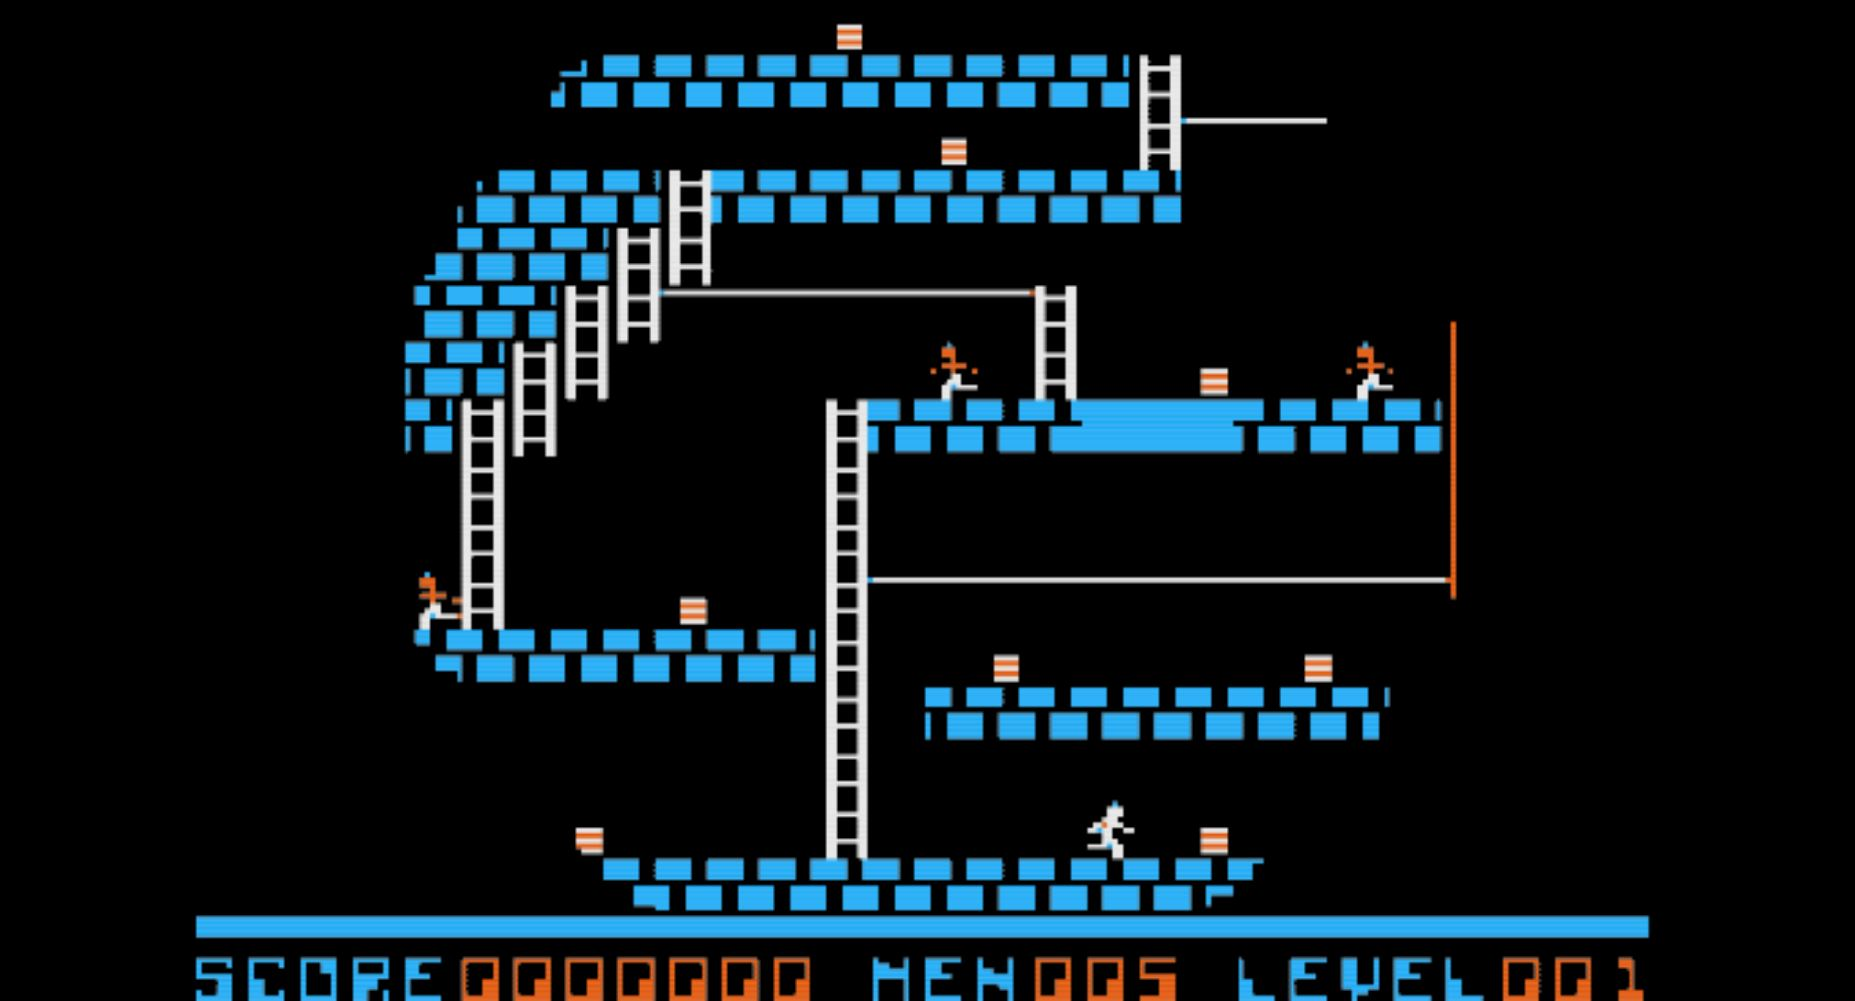
\includegraphics[width=\columnwidth]{iris}

\nwenddocs{}\nwbegincode{138}\sublabel{NW1Xx3lK-10jlgu-I}\nwmargintag{{\nwtagstyle{}\subpageref{NW1Xx3lK-10jlgu-I}}}\moddef{defines~{\nwtagstyle{}\subpageref{NW1Xx3lK-10jlgu-1}}}\plusendmoddef\nwstartdeflinemarkup\nwusesondefline{\\{NW1Xx3lK-1p0Y9w-1}}\nwprevnextdefs{NW1Xx3lK-10jlgu-H}{NW1Xx3lK-10jlgu-J}\nwenddeflinemarkup
\nwlinkedidentc{WIPE_COUNTER}{NW1Xx3lK-10jlgu-I}        EQU     $6D
\nwlinkedidentc{WIPE_MODE}{NW1Xx3lK-10jlgu-I}           EQU     $A5     ; 0 for open, 1 for close.
WIPE_DIR            EQU     $72     ; 0 for close, 1 for open.
WIPE_CENTER_X       EQU     $77
WIPE_CENTER_Y       EQU     $73
\nwindexdefn{\nwixident{WIPE{\_}COUNTER}}{WIPE:unCOUNTER}{NW1Xx3lK-10jlgu-I}\nwindexdefn{\nwixident{WIPE{\_}MODE}}{WIPE:unMODE}{NW1Xx3lK-10jlgu-I}\eatline
\nwused{\\{NW1Xx3lK-1p0Y9w-1}}\nwidentdefs{\\{{\nwixident{WIPE{\_}COUNTER}}{WIPE:unCOUNTER}}\\{{\nwixident{WIPE{\_}MODE}}{WIPE:unMODE}}}\nwendcode{}\nwbegindocs{139}\nwdocspar
\nwenddocs{}\nwbegincode{140}\sublabel{NW1Xx3lK-6p0m3-1}\nwmargintag{{\nwtagstyle{}\subpageref{NW1Xx3lK-6p0m3-1}}}\moddef{iris wipe~{\nwtagstyle{}\subpageref{NW1Xx3lK-6p0m3-1}}}\endmoddef\nwstartdeflinemarkup\nwusesondefline{\\{NW1Xx3lK-8jv1b-K}}\nwenddeflinemarkup
    ORG     $88A2
\nwlinkedidentc{IRIS_WIPE}{NW1Xx3lK-6p0m3-1}:
    SUBROUTINE

    LDA     88
    STA     WIPE_CENTER_Y
    LDA     140
    STA     WIPE_CENTER_X

    LDA     \nwlinkedidentc{WIPE_MODE}{NW1Xx3lK-10jlgu-I}
    BEQ     .iris_open

    LDX     #$AA
    STX     \nwlinkedidentc{WIPE_COUNTER}{NW1Xx3lK-10jlgu-I}
    LDX     #$00
    STX     WIPE_DIR             ; Close

.loop_close:
    JSR     \nwlinkedidentc{IRIS_WIPE_STEP}{NW1Xx3lK-1tGalf-1}
    DEC     \nwlinkedidentc{WIPE_COUNTER}{NW1Xx3lK-10jlgu-I}
    BNE     .loop_close

.iris_open:
    LDA     #$01
    STA     \nwlinkedidentc{WIPE_COUNTER}{NW1Xx3lK-10jlgu-I}
    STA     \nwlinkedidentc{WIPE_MODE}{NW1Xx3lK-10jlgu-I}           ; So next time we will close.
    STA     WIPE_DIR            ; Open
    JSR     \nwlinkedidentc{PUT_STATUS_LIVES}{NW1Xx3lK-8jv1b-I}
    JSR     \nwlinkedidentc{PUT_STATUS_LEVEL}{NW1Xx3lK-8jv1b-I}

.loop_open:
    JSR     \nwlinkedidentc{IRIS_WIPE_STEP}{NW1Xx3lK-1tGalf-1}
    INC     \nwlinkedidentc{WIPE_COUNTER}{NW1Xx3lK-10jlgu-I}
    LDA     \nwlinkedidentc{WIPE_COUNTER}{NW1Xx3lK-10jlgu-I}
    CMP     #$AA
    BNE     .loop_open
    RTS
\nwindexdefn{\nwixident{IRIS{\_}WIPE}}{IRIS:unWIPE}{NW1Xx3lK-6p0m3-1}\eatline
\nwused{\\{NW1Xx3lK-8jv1b-K}}\nwidentdefs{\\{{\nwixident{IRIS{\_}WIPE}}{IRIS:unWIPE}}}\nwidentuses{\\{{\nwixident{IRIS{\_}WIPE{\_}STEP}}{IRIS:unWIPE:unSTEP}}\\{{\nwixident{PUT{\_}STATUS{\_}LEVEL}}{PUT:unSTATUS:unLEVEL}}\\{{\nwixident{PUT{\_}STATUS{\_}LIVES}}{PUT:unSTATUS:unLIVES}}\\{{\nwixident{WIPE{\_}COUNTER}}{WIPE:unCOUNTER}}\\{{\nwixident{WIPE{\_}MODE}}{WIPE:unMODE}}}\nwindexuse{\nwixident{IRIS{\_}WIPE{\_}STEP}}{IRIS:unWIPE:unSTEP}{NW1Xx3lK-6p0m3-1}\nwindexuse{\nwixident{PUT{\_}STATUS{\_}LEVEL}}{PUT:unSTATUS:unLEVEL}{NW1Xx3lK-6p0m3-1}\nwindexuse{\nwixident{PUT{\_}STATUS{\_}LIVES}}{PUT:unSTATUS:unLIVES}{NW1Xx3lK-6p0m3-1}\nwindexuse{\nwixident{WIPE{\_}COUNTER}}{WIPE:unCOUNTER}{NW1Xx3lK-6p0m3-1}\nwindexuse{\nwixident{WIPE{\_}MODE}}{WIPE:unMODE}{NW1Xx3lK-6p0m3-1}\nwendcode{}\nwbegindocs{141}\nwdocspar
The routine {\Tt{}\nwlinkedidentq{IRIS{\_}WIPE{\_}STEP}{NW1Xx3lK-1tGalf-1}\nwendquote} does a lot of math to compute the circular iris, all parameterized
on {\Tt{}\nwlinkedidentq{WIPE{\_}COUNTER}{NW1Xx3lK-10jlgu-I}\nwendquote}.

Here is a routine that divides a 16-bit value in A and X (X being LSB) by 7, storing the
result in Y, with remainder in A. The routine effectively does long division. It also uses two temporaries.

\nwenddocs{}\nwbegincode{142}\sublabel{NW1Xx3lK-10jlgu-J}\nwmargintag{{\nwtagstyle{}\subpageref{NW1Xx3lK-10jlgu-J}}}\moddef{defines~{\nwtagstyle{}\subpageref{NW1Xx3lK-10jlgu-1}}}\plusendmoddef\nwstartdeflinemarkup\nwusesondefline{\\{NW1Xx3lK-1p0Y9w-1}}\nwprevnextdefs{NW1Xx3lK-10jlgu-I}{NW1Xx3lK-10jlgu-K}\nwenddeflinemarkup
\nwlinkedidentc{MATH_TMPL}{NW1Xx3lK-10jlgu-J}     EQU     $6F
\nwlinkedidentc{MATH_TMPH}{NW1Xx3lK-10jlgu-J}     EQU     $70
\nwindexdefn{\nwixident{MATH{\_}TMPL}}{MATH:unTMPL}{NW1Xx3lK-10jlgu-J}\nwindexdefn{\nwixident{MATH{\_}TMPH}}{MATH:unTMPH}{NW1Xx3lK-10jlgu-J}\eatline
\nwused{\\{NW1Xx3lK-1p0Y9w-1}}\nwidentdefs{\\{{\nwixident{MATH{\_}TMPH}}{MATH:unTMPH}}\\{{\nwixident{MATH{\_}TMPL}}{MATH:unTMPL}}}\nwendcode{}\nwbegindocs{143}\nwdocspar
\nwenddocs{}\nwbegincode{144}\sublabel{NW1Xx3lK-8jv1b-J}\nwmargintag{{\nwtagstyle{}\subpageref{NW1Xx3lK-8jv1b-J}}}\moddef{routines~{\nwtagstyle{}\subpageref{NW1Xx3lK-8jv1b-1}}}\plusendmoddef\nwstartdeflinemarkup\nwusesondefline{\\{NW1Xx3lK-1p0Y9w-1}}\nwprevnextdefs{NW1Xx3lK-8jv1b-I}{NW1Xx3lK-8jv1b-K}\nwenddeflinemarkup
    ORG     $8A45
\nwlinkedidentc{DIV_BY_7}{NW1Xx3lK-8jv1b-J}:
    SUBROUTINE
    ; Enter routine with AX set to (unsigned) numerator.
    ; On exit, Y will contain the integer portion of AX/7,
    ; and A contains the remainder.

    STX     \nwlinkedidentc{MATH_TMPL}{NW1Xx3lK-10jlgu-J}
    LDY     8
    SEC
    SBC     7

.loop:
    PHP
    ROL     \nwlinkedidentc{MATH_TMPH}{NW1Xx3lK-10jlgu-J}
    ASL     \nwlinkedidentc{MATH_TMPL}{NW1Xx3lK-10jlgu-J}
    ROL
    PLP
    BCC     .adjust_up
    SBC     7
    JMP     .next

.adjust_up
    ADC     7

.next
    DEY
    BNE     .loop

    BCS     .no_adjust
    ADC     7
    CLC

.no_adjust
    ROL     \nwlinkedidentc{MATH_TMPH}{NW1Xx3lK-10jlgu-J}
    LDY     \nwlinkedidentc{MATH_TMPH}{NW1Xx3lK-10jlgu-J}
    RTS
\nwindexdefn{\nwixident{DIV{\_}BY{\_}7}}{DIV:unBY:un7}{NW1Xx3lK-8jv1b-J}\eatline
\nwused{\\{NW1Xx3lK-1p0Y9w-1}}\nwidentdefs{\\{{\nwixident{DIV{\_}BY{\_}7}}{DIV:unBY:un7}}}\nwidentuses{\\{{\nwixident{MATH{\_}TMPH}}{MATH:unTMPH}}\\{{\nwixident{MATH{\_}TMPL}}{MATH:unTMPL}}}\nwindexuse{\nwixident{MATH{\_}TMPH}}{MATH:unTMPH}{NW1Xx3lK-8jv1b-J}\nwindexuse{\nwixident{MATH{\_}TMPL}}{MATH:unTMPL}{NW1Xx3lK-8jv1b-J}\nwendcode{}\nwbegindocs{145}\nwdocspar
Now, for one iris wipe step, we will need lots and lots of temporaries.

\nwenddocs{}\nwbegincode{146}\sublabel{NW1Xx3lK-10jlgu-K}\nwmargintag{{\nwtagstyle{}\subpageref{NW1Xx3lK-10jlgu-K}}}\moddef{defines~{\nwtagstyle{}\subpageref{NW1Xx3lK-10jlgu-1}}}\plusendmoddef\nwstartdeflinemarkup\nwusesondefline{\\{NW1Xx3lK-1p0Y9w-1}}\nwprevnextdefs{NW1Xx3lK-10jlgu-J}{NW1Xx3lK-10jlgu-L}\nwenddeflinemarkup
\nwlinkedidentc{WIPE0}{NW1Xx3lK-10jlgu-K}       EQU     $69     ; 16-bit value
\nwlinkedidentc{WIPE1}{NW1Xx3lK-10jlgu-K}       EQU     $67     ; 16-bit value
\nwlinkedidentc{WIPE2}{NW1Xx3lK-10jlgu-K}       EQU     $6B     ; 16-bit value
\nwlinkedidentc{WIPE3L}{NW1Xx3lK-10jlgu-K}      EQU     $75
\nwlinkedidentc{WIPE4L}{NW1Xx3lK-10jlgu-K}      EQU     $76
\nwlinkedidentc{WIPE5L}{NW1Xx3lK-10jlgu-K}      EQU     $77
\nwlinkedidentc{WIPE6L}{NW1Xx3lK-10jlgu-K}      EQU     $78
\nwlinkedidentc{WIPE3H}{NW1Xx3lK-10jlgu-K}      EQU     $79
\nwlinkedidentc{WIPE4H}{NW1Xx3lK-10jlgu-K}      EQU     $7A
\nwlinkedidentc{WIPE5H}{NW1Xx3lK-10jlgu-K}      EQU     $7B
\nwlinkedidentc{WIPE6H}{NW1Xx3lK-10jlgu-K}      EQU     $7C
\nwlinkedidentc{WIPE7D}{NW1Xx3lK-10jlgu-K}      EQU     $7D     ; Dividends
\nwlinkedidentc{WIPE8D}{NW1Xx3lK-10jlgu-K}      EQU     $7E
\nwlinkedidentc{WIPE9D}{NW1Xx3lK-10jlgu-K}      EQU     $7F
\nwlinkedidentc{WIPE10D}{NW1Xx3lK-10jlgu-K}     EQU     $80
\nwlinkedidentc{WIPE7R}{NW1Xx3lK-10jlgu-K}      EQU     $81     ; Remainders
\nwlinkedidentc{WIPE8R}{NW1Xx3lK-10jlgu-K}      EQU     $82
\nwlinkedidentc{WIPE9R}{NW1Xx3lK-10jlgu-K}      EQU     $83
\nwlinkedidentc{WIPE10R}{NW1Xx3lK-10jlgu-K}     EQU     $84
\nwindexdefn{\nwixident{WIPE0}}{WIPE0}{NW1Xx3lK-10jlgu-K}\nwindexdefn{\nwixident{WIPE1}}{WIPE1}{NW1Xx3lK-10jlgu-K}\nwindexdefn{\nwixident{WIPE2}}{WIPE2}{NW1Xx3lK-10jlgu-K}\nwindexdefn{\nwixident{WIPE3L}}{WIPE3L}{NW1Xx3lK-10jlgu-K}\nwindexdefn{\nwixident{WIPE3H}}{WIPE3H}{NW1Xx3lK-10jlgu-K}\nwindexdefn{\nwixident{WIPE4L}}{WIPE4L}{NW1Xx3lK-10jlgu-K}\nwindexdefn{\nwixident{WIPE4H}}{WIPE4H}{NW1Xx3lK-10jlgu-K}\nwindexdefn{\nwixident{WIPE5L}}{WIPE5L}{NW1Xx3lK-10jlgu-K}\nwindexdefn{\nwixident{WIPE5H}}{WIPE5H}{NW1Xx3lK-10jlgu-K}\nwindexdefn{\nwixident{WIPE6L}}{WIPE6L}{NW1Xx3lK-10jlgu-K}\nwindexdefn{\nwixident{WIPE6H}}{WIPE6H}{NW1Xx3lK-10jlgu-K}\nwindexdefn{\nwixident{WIPE7D}}{WIPE7D}{NW1Xx3lK-10jlgu-K}\nwindexdefn{\nwixident{WIPE7R}}{WIPE7R}{NW1Xx3lK-10jlgu-K}\nwindexdefn{\nwixident{WIPE8D}}{WIPE8D}{NW1Xx3lK-10jlgu-K}\nwindexdefn{\nwixident{WIPE8R}}{WIPE8R}{NW1Xx3lK-10jlgu-K}\nwindexdefn{\nwixident{WIPE9D}}{WIPE9D}{NW1Xx3lK-10jlgu-K}\nwindexdefn{\nwixident{WIPE9R}}{WIPE9R}{NW1Xx3lK-10jlgu-K}\nwindexdefn{\nwixident{WIPE10D}}{WIPE10D}{NW1Xx3lK-10jlgu-K}\nwindexdefn{\nwixident{WIPE10R}}{WIPE10R}{NW1Xx3lK-10jlgu-K}\eatline
\nwused{\\{NW1Xx3lK-1p0Y9w-1}}\nwidentdefs{\\{{\nwixident{WIPE0}}{WIPE0}}\\{{\nwixident{WIPE1}}{WIPE1}}\\{{\nwixident{WIPE10D}}{WIPE10D}}\\{{\nwixident{WIPE10R}}{WIPE10R}}\\{{\nwixident{WIPE2}}{WIPE2}}\\{{\nwixident{WIPE3H}}{WIPE3H}}\\{{\nwixident{WIPE3L}}{WIPE3L}}\\{{\nwixident{WIPE4H}}{WIPE4H}}\\{{\nwixident{WIPE4L}}{WIPE4L}}\\{{\nwixident{WIPE5H}}{WIPE5H}}\\{{\nwixident{WIPE5L}}{WIPE5L}}\\{{\nwixident{WIPE6H}}{WIPE6H}}\\{{\nwixident{WIPE6L}}{WIPE6L}}\\{{\nwixident{WIPE7D}}{WIPE7D}}\\{{\nwixident{WIPE7R}}{WIPE7R}}\\{{\nwixident{WIPE8D}}{WIPE8D}}\\{{\nwixident{WIPE8R}}{WIPE8R}}\\{{\nwixident{WIPE9D}}{WIPE9D}}\\{{\nwixident{WIPE9R}}{WIPE9R}}}\nwendcode{}\nwbegindocs{147}\nwdocspar
The first thing we do for a single step is initialize all those variables!

\nwenddocs{}\nwbegincode{148}\sublabel{NW1Xx3lK-1tGalf-1}\nwmargintag{{\nwtagstyle{}\subpageref{NW1Xx3lK-1tGalf-1}}}\moddef{iris wipe step~{\nwtagstyle{}\subpageref{NW1Xx3lK-1tGalf-1}}}\endmoddef\nwstartdeflinemarkup\nwusesondefline{\\{NW1Xx3lK-8jv1b-K}}\nwprevnextdefs{\relax}{NW1Xx3lK-1tGalf-2}\nwenddeflinemarkup
    ORG     $88D7
\nwlinkedidentc{IRIS_WIPE_STEP}{NW1Xx3lK-1tGalf-1}:
    SUBROUTINE

\LA{}\code{}WIPE0\ =\ WIPE{\_}COUNTER\edoc{}~{\nwtagstyle{}\subpageref{NW1Xx3lK-2Rx43B-1}}\RA{}
\LA{}\code{}WIPE1\ =\ 0\edoc{}~{\nwtagstyle{}\subpageref{NW1Xx3lK-1ZlBVV-1}}\RA{}
\LA{}\code{}WIPE2\ =\ 2\ *\ WIPE0\edoc{}~{\nwtagstyle{}\subpageref{NW1Xx3lK-39zOBY-1}}\RA{}
\LA{}\code{}WIPE2\ =\ 3\ -\ WIPE2\edoc{}~{\nwtagstyle{}\subpageref{NW1Xx3lK-1Ny5Ce-1}}\RA{}

; WIPE3, WIPE4, WIPE5, and WIPE6 correspond to
; row numbers. WIPE3 is above the center, WIPE6
; is below the center, while WIPE4 and WIPE5 are on
; the center.

\LA{}\code{}WIPE3\ =\ WIPE{\_}CENTER{\_}Y\ -\ WIPE{\_}COUNTER\edoc{}~{\nwtagstyle{}\subpageref{NW1Xx3lK-3R5hBF-1}}\RA{}
\LA{}\code{}WIPE4\ =\ WIPE5\ =\ WIPE{\_}CENTER{\_}Y\edoc{}~{\nwtagstyle{}\subpageref{NW1Xx3lK-2JOPWw-1}}\RA{}
\LA{}\code{}WIPE6\ =\ WIPE{\_}CENTER{\_}Y\ +\ WIPE{\_}COUNTER\edoc{}~{\nwtagstyle{}\subpageref{NW1Xx3lK-4TkslJ-1}}\RA{}

; WIPE7, WIPE8, WIPE9, and WIPE10 correspond to
; column byte numbers. Note the division by 7 pixels!
; WIPE7 is left of center, WIPE10 is right of center,
; while WIPE8 and WIPE9 are on the center.

\LA{}\code{}WIPE7\ =\ (WIPE{\_}CENTER{\_}X\ -\ WIPE{\_}COUNTER)\ /\ 7\edoc{}~{\nwtagstyle{}\subpageref{NW1Xx3lK-2ojStX-1}}\RA{}
\LA{}\code{}WIPE8\ =\ WIPE9\ =\ WIPE{\_}CENTER{\_}X\ /\ 7\edoc{}~{\nwtagstyle{}\subpageref{NW1Xx3lK-2QGdSi-1}}\RA{}
\LA{}\code{}WIPE10\ =\ (WIPE{\_}CENTER{\_}X\ +\ WIPE{\_}COUNTER)\ /\ 7\edoc{}~{\nwtagstyle{}\subpageref{NW1Xx3lK-2Um1dk-1}}\RA{}
\nwindexdefn{\nwixident{IRIS{\_}WIPE{\_}STEP}}{IRIS:unWIPE:unSTEP}{NW1Xx3lK-1tGalf-1}\eatline
\nwalsodefined{\\{NW1Xx3lK-1tGalf-2}}\nwused{\\{NW1Xx3lK-8jv1b-K}}\nwidentdefs{\\{{\nwixident{IRIS{\_}WIPE{\_}STEP}}{IRIS:unWIPE:unSTEP}}}\nwendcode{}\nwbegindocs{149}\nwdocspar
Now we loop. This involves checking {\Tt{}\nwlinkedidentq{WIPE1}{NW1Xx3lK-10jlgu-K}\nwendquote} against {\Tt{}\nwlinkedidentq{WIPE0}{NW1Xx3lK-10jlgu-K}\nwendquote}:

\begin{itemize}
  \item If {\Tt{}\nwlinkedidentq{WIPE1}{NW1Xx3lK-10jlgu-K}\nwendquote} $<$ {\Tt{}\nwlinkedidentq{WIPE0}{NW1Xx3lK-10jlgu-K}\nwendquote}, return.
  \item If {\Tt{}\nwlinkedidentq{WIPE1}{NW1Xx3lK-10jlgu-K}\nwendquote} == {\Tt{}\nwlinkedidentq{WIPE0}{NW1Xx3lK-10jlgu-K}\nwendquote}, go to {\Tt{}\nwlinkedidentq{DRAW{\_}WIPE{\_}STEP}{NW1Xx3lK-1DtO18-1}\nwendquote} then return.
  \item Otherwise, call {\Tt{}\nwlinkedidentq{DRAW{\_}WIPE{\_}STEP}{NW1Xx3lK-1DtO18-1}\nwendquote} and go round the loop.
\end{itemize}

Going around the loop involves calling {\Tt{}\nwlinkedidentq{DRAW{\_}WIPE{\_}STEP}{NW1Xx3lK-1DtO18-1}\nwendquote}, then adjusting
the numbers.

\nwenddocs{}\nwbegincode{150}\sublabel{NW1Xx3lK-1tGalf-2}\nwmargintag{{\nwtagstyle{}\subpageref{NW1Xx3lK-1tGalf-2}}}\moddef{iris wipe step~{\nwtagstyle{}\subpageref{NW1Xx3lK-1tGalf-1}}}\plusendmoddef\nwstartdeflinemarkup\nwusesondefline{\\{NW1Xx3lK-8jv1b-K}}\nwprevnextdefs{NW1Xx3lK-1tGalf-1}{\relax}\nwenddeflinemarkup
.loop:

\LA{}iris wipe loop check~{\nwtagstyle{}\subpageref{NW1Xx3lK-3vxyMm-1}}\RA{}

    JSR     \nwlinkedidentc{DRAW_WIPE_STEP}{NW1Xx3lK-1DtO18-1}

    LDA     \nwlinkedidentc{WIPE2}{NW1Xx3lK-10jlgu-K}+1
    BPL     .89a7

\LA{}\code{}WIPE2\ +=\ 4\ *\ WIPE1\ +\ 6\edoc{}~{\nwtagstyle{}\subpageref{NW1Xx3lK-mcL2B-1}}\RA{}
    JMP     .8a14

.89a7:

\LA{}\code{}WIPE2\ +=\ 4\ *\ (WIPE1\ -\ WIPE0)\ +\ 16\edoc{}~{\nwtagstyle{}\subpageref{NW1Xx3lK-2eL1Rw-1}}\RA{}
\LA{}Decrement \code{}WIPE0\edoc{}~{\nwtagstyle{}\subpageref{NW1Xx3lK-2u2rZr-1}}\RA{}
\LA{}Increment \code{}WIPE3\edoc{}~{\nwtagstyle{}\subpageref{NW1Xx3lK-13RMM3-1}}\RA{}
\LA{}Decrement \code{}WIPE10\edoc{} modulo 7~{\nwtagstyle{}\subpageref{NW1Xx3lK-11REH7-1}}\RA{}
\LA{}Increment \code{}WIPE7\edoc{} modulo 7~{\nwtagstyle{}\subpageref{NW1Xx3lK-11uG8h-1}}\RA{}
\LA{}Decrement \code{}WIPE6\edoc{}~{\nwtagstyle{}\subpageref{NW1Xx3lK-2u2n6B-1}}\RA{}

.8a14:

\LA{}Increment \code{}WIPE1\edoc{}~{\nwtagstyle{}\subpageref{NW1Xx3lK-13RECF-1}}\RA{}
\LA{}Increment \code{}WIPE9\edoc{} modulo 7~{\nwtagstyle{}\subpageref{NW1Xx3lK-3Y2gMs-1}}\RA{}
\LA{}Decrement \code{}WIPE4\edoc{}~{\nwtagstyle{}\subpageref{NW1Xx3lK-2u2srL-1}}\RA{}
\LA{}Increment \code{}WIPE5\edoc{}~{\nwtagstyle{}\subpageref{NW1Xx3lK-13RI6p-1}}\RA{}
\LA{}Decrement \code{}WIPE8\edoc{} modulo 7~{\nwtagstyle{}\subpageref{NW1Xx3lK-nzt1T-1}}\RA{}
    JMP     .loop
\nwused{\\{NW1Xx3lK-8jv1b-K}}\nwidentuses{\\{{\nwixident{DRAW{\_}WIPE{\_}STEP}}{DRAW:unWIPE:unSTEP}}\\{{\nwixident{WIPE2}}{WIPE2}}}\nwindexuse{\nwixident{DRAW{\_}WIPE{\_}STEP}}{DRAW:unWIPE:unSTEP}{NW1Xx3lK-1tGalf-2}\nwindexuse{\nwixident{WIPE2}}{WIPE2}{NW1Xx3lK-1tGalf-2}\nwendcode{}\nwbegindocs{151}\nwdocspar

Drawing a wipe step draws all four parts. There are two rows which move north
and two rows that move south. There are also two left and right offsets, one
short and one long. This makes eight combinations.

\nwenddocs{}\nwbegincode{152}\sublabel{NW1Xx3lK-1DtO18-1}\nwmargintag{{\nwtagstyle{}\subpageref{NW1Xx3lK-1DtO18-1}}}\moddef{draw wipe step~{\nwtagstyle{}\subpageref{NW1Xx3lK-1DtO18-1}}}\endmoddef\nwstartdeflinemarkup\nwusesondefline{\\{NW1Xx3lK-8jv1b-K}}\nwenddeflinemarkup
    ORG     $8A69
\nwlinkedidentc{DRAW_WIPE_STEP}{NW1Xx3lK-1DtO18-1}:
    SUBROUTINE

\LA{}Draw wipe for south part~{\nwtagstyle{}\subpageref{NW1Xx3lK-29jG99-1}}\RA{}
\LA{}Draw wipe for north part~{\nwtagstyle{}\subpageref{NW1Xx3lK-29yoMR-1}}\RA{}
\LA{}Draw wipe for north2 part~{\nwtagstyle{}\subpageref{NW1Xx3lK-3AjGdu-1}}\RA{}
\LA{}Draw wipe for south2 part~{\nwtagstyle{}\subpageref{NW1Xx3lK-3OCJye-1}}\RA{}
\nwindexdefn{\nwixident{DRAW{\_}WIPE{\_}STEP}}{DRAW:unWIPE:unSTEP}{NW1Xx3lK-1DtO18-1}\eatline
\nwused{\\{NW1Xx3lK-8jv1b-K}}\nwidentdefs{\\{{\nwixident{DRAW{\_}WIPE{\_}STEP}}{DRAW:unWIPE:unSTEP}}}\nwendcode{}\nwbegindocs{153}\nwdocspar
Each part consists of two halves, right and left (or east and west).

\nwenddocs{}\nwbegincode{154}\sublabel{NW1Xx3lK-29jG99-1}\nwmargintag{{\nwtagstyle{}\subpageref{NW1Xx3lK-29jG99-1}}}\moddef{Draw wipe for south part~{\nwtagstyle{}\subpageref{NW1Xx3lK-29jG99-1}}}\endmoddef\nwstartdeflinemarkup\nwusesondefline{\\{NW1Xx3lK-1DtO18-1}}\nwenddeflinemarkup
    LDY     \nwlinkedidentc{WIPE6H}{NW1Xx3lK-10jlgu-K}
    BNE     .draw_north
    LDY     \nwlinkedidentc{WIPE6L}{NW1Xx3lK-10jlgu-K}
    CPY     176
    BCS     .draw_north        ; Skip if WIPE6 >= 176

    JSR     \nwlinkedidentc{ROW_TO_ADDR_FOR_BOTH_PAGES}{NW1Xx3lK-8jv1b-4}

    ; East side
    LDY     \nwlinkedidentc{WIPE9D}{NW1Xx3lK-10jlgu-K}
    CPY     40
    BCS     .draw_south_west
    LDX     \nwlinkedidentc{WIPE9R}{NW1Xx3lK-10jlgu-K}
    JSR     \nwlinkedidentc{DRAW_WIPE_BLOCK}{NW1Xx3lK-32wUsj-1}

.draw_south_west
    ; West side
    LDY     \nwlinkedidentc{WIPE8D}{NW1Xx3lK-10jlgu-K}
    CPY     40
    BCS     .draw_north
    LDX     \nwlinkedidentc{WIPE9R}{NW1Xx3lK-10jlgu-K}
    JSR     \nwlinkedidentc{DRAW_WIPE_BLOCK}{NW1Xx3lK-32wUsj-1}
\nwused{\\{NW1Xx3lK-1DtO18-1}}\nwidentuses{\\{{\nwixident{DRAW{\_}WIPE{\_}BLOCK}}{DRAW:unWIPE:unBLOCK}}\\{{\nwixident{ROW{\_}TO{\_}ADDR{\_}FOR{\_}BOTH{\_}PAGES}}{ROW:unTO:unADDR:unFOR:unBOTH:unPAGES}}\\{{\nwixident{WIPE6H}}{WIPE6H}}\\{{\nwixident{WIPE6L}}{WIPE6L}}\\{{\nwixident{WIPE8D}}{WIPE8D}}\\{{\nwixident{WIPE9D}}{WIPE9D}}\\{{\nwixident{WIPE9R}}{WIPE9R}}}\nwindexuse{\nwixident{DRAW{\_}WIPE{\_}BLOCK}}{DRAW:unWIPE:unBLOCK}{NW1Xx3lK-29jG99-1}\nwindexuse{\nwixident{ROW{\_}TO{\_}ADDR{\_}FOR{\_}BOTH{\_}PAGES}}{ROW:unTO:unADDR:unFOR:unBOTH:unPAGES}{NW1Xx3lK-29jG99-1}\nwindexuse{\nwixident{WIPE6H}}{WIPE6H}{NW1Xx3lK-29jG99-1}\nwindexuse{\nwixident{WIPE6L}}{WIPE6L}{NW1Xx3lK-29jG99-1}\nwindexuse{\nwixident{WIPE8D}}{WIPE8D}{NW1Xx3lK-29jG99-1}\nwindexuse{\nwixident{WIPE9D}}{WIPE9D}{NW1Xx3lK-29jG99-1}\nwindexuse{\nwixident{WIPE9R}}{WIPE9R}{NW1Xx3lK-29jG99-1}\nwendcode{}\nwbegindocs{155}\nwdocspar

\nwenddocs{}\nwbegincode{156}\sublabel{NW1Xx3lK-29yoMR-1}\nwmargintag{{\nwtagstyle{}\subpageref{NW1Xx3lK-29yoMR-1}}}\moddef{Draw wipe for north part~{\nwtagstyle{}\subpageref{NW1Xx3lK-29yoMR-1}}}\endmoddef\nwstartdeflinemarkup\nwusesondefline{\\{NW1Xx3lK-1DtO18-1}}\nwenddeflinemarkup
.draw_north:
    LDY     \nwlinkedidentc{WIPE3H}{NW1Xx3lK-10jlgu-K}
    BNE     .draw_north2
    LDY     \nwlinkedidentc{WIPE3L}{NW1Xx3lK-10jlgu-K}
    CPY     176
    BCS     .draw_north2        ; Skip if WIPE3 >= 176

    JSR     \nwlinkedidentc{ROW_TO_ADDR_FOR_BOTH_PAGES}{NW1Xx3lK-8jv1b-4}

    ; East side
    LDY     \nwlinkedidentc{WIPE9D}{NW1Xx3lK-10jlgu-K}
    CPY     40
    BCS     .draw_north_west
    LDX     \nwlinkedidentc{WIPE9R}{NW1Xx3lK-10jlgu-K}
    JSR     \nwlinkedidentc{DRAW_WIPE_BLOCK}{NW1Xx3lK-32wUsj-1}

.draw_north_west
    ; West side
    LDY     \nwlinkedidentc{WIPE8D}{NW1Xx3lK-10jlgu-K}
    CPY     40
    BCS     .draw_north2
    LDX     \nwlinkedidentc{WIPE9R}{NW1Xx3lK-10jlgu-K}
    JSR     \nwlinkedidentc{DRAW_WIPE_BLOCK}{NW1Xx3lK-32wUsj-1}
\nwused{\\{NW1Xx3lK-1DtO18-1}}\nwidentuses{\\{{\nwixident{DRAW{\_}WIPE{\_}BLOCK}}{DRAW:unWIPE:unBLOCK}}\\{{\nwixident{ROW{\_}TO{\_}ADDR{\_}FOR{\_}BOTH{\_}PAGES}}{ROW:unTO:unADDR:unFOR:unBOTH:unPAGES}}\\{{\nwixident{WIPE3H}}{WIPE3H}}\\{{\nwixident{WIPE3L}}{WIPE3L}}\\{{\nwixident{WIPE8D}}{WIPE8D}}\\{{\nwixident{WIPE9D}}{WIPE9D}}\\{{\nwixident{WIPE9R}}{WIPE9R}}}\nwindexuse{\nwixident{DRAW{\_}WIPE{\_}BLOCK}}{DRAW:unWIPE:unBLOCK}{NW1Xx3lK-29yoMR-1}\nwindexuse{\nwixident{ROW{\_}TO{\_}ADDR{\_}FOR{\_}BOTH{\_}PAGES}}{ROW:unTO:unADDR:unFOR:unBOTH:unPAGES}{NW1Xx3lK-29yoMR-1}\nwindexuse{\nwixident{WIPE3H}}{WIPE3H}{NW1Xx3lK-29yoMR-1}\nwindexuse{\nwixident{WIPE3L}}{WIPE3L}{NW1Xx3lK-29yoMR-1}\nwindexuse{\nwixident{WIPE8D}}{WIPE8D}{NW1Xx3lK-29yoMR-1}\nwindexuse{\nwixident{WIPE9D}}{WIPE9D}{NW1Xx3lK-29yoMR-1}\nwindexuse{\nwixident{WIPE9R}}{WIPE9R}{NW1Xx3lK-29yoMR-1}\nwendcode{}\nwbegindocs{157}\nwdocspar

\nwenddocs{}\nwbegincode{158}\sublabel{NW1Xx3lK-3AjGdu-1}\nwmargintag{{\nwtagstyle{}\subpageref{NW1Xx3lK-3AjGdu-1}}}\moddef{Draw wipe for north2 part~{\nwtagstyle{}\subpageref{NW1Xx3lK-3AjGdu-1}}}\endmoddef\nwstartdeflinemarkup\nwusesondefline{\\{NW1Xx3lK-1DtO18-1}}\nwenddeflinemarkup
.draw_north2:
    LDY     \nwlinkedidentc{WIPE5H}{NW1Xx3lK-10jlgu-K}
    BNE     .draw_south2
    LDY     \nwlinkedidentc{WIPE5L}{NW1Xx3lK-10jlgu-K}
    CPY     176
    BCS     .draw_south2        ; Skip if WIPE5 >= 176

    JSR     \nwlinkedidentc{ROW_TO_ADDR_FOR_BOTH_PAGES}{NW1Xx3lK-8jv1b-4}

    ; East side
    LDY     \nwlinkedidentc{WIPE10D}{NW1Xx3lK-10jlgu-K}
    CPY     40
    BCS     .draw_north2_west
    LDX     \nwlinkedidentc{WIPE10R}{NW1Xx3lK-10jlgu-K}
    JSR     \nwlinkedidentc{DRAW_WIPE_BLOCK}{NW1Xx3lK-32wUsj-1}

.draw_north2_west
    ; West side
    LDY     \nwlinkedidentc{WIPE7D}{NW1Xx3lK-10jlgu-K}
    CPY     40
    BCS     .draw_south2
    LDX     \nwlinkedidentc{WIPE7R}{NW1Xx3lK-10jlgu-K}
    JSR     \nwlinkedidentc{DRAW_WIPE_BLOCK}{NW1Xx3lK-32wUsj-1}
\nwused{\\{NW1Xx3lK-1DtO18-1}}\nwidentuses{\\{{\nwixident{DRAW{\_}WIPE{\_}BLOCK}}{DRAW:unWIPE:unBLOCK}}\\{{\nwixident{ROW{\_}TO{\_}ADDR{\_}FOR{\_}BOTH{\_}PAGES}}{ROW:unTO:unADDR:unFOR:unBOTH:unPAGES}}\\{{\nwixident{WIPE10D}}{WIPE10D}}\\{{\nwixident{WIPE10R}}{WIPE10R}}\\{{\nwixident{WIPE5H}}{WIPE5H}}\\{{\nwixident{WIPE5L}}{WIPE5L}}\\{{\nwixident{WIPE7D}}{WIPE7D}}\\{{\nwixident{WIPE7R}}{WIPE7R}}}\nwindexuse{\nwixident{DRAW{\_}WIPE{\_}BLOCK}}{DRAW:unWIPE:unBLOCK}{NW1Xx3lK-3AjGdu-1}\nwindexuse{\nwixident{ROW{\_}TO{\_}ADDR{\_}FOR{\_}BOTH{\_}PAGES}}{ROW:unTO:unADDR:unFOR:unBOTH:unPAGES}{NW1Xx3lK-3AjGdu-1}\nwindexuse{\nwixident{WIPE10D}}{WIPE10D}{NW1Xx3lK-3AjGdu-1}\nwindexuse{\nwixident{WIPE10R}}{WIPE10R}{NW1Xx3lK-3AjGdu-1}\nwindexuse{\nwixident{WIPE5H}}{WIPE5H}{NW1Xx3lK-3AjGdu-1}\nwindexuse{\nwixident{WIPE5L}}{WIPE5L}{NW1Xx3lK-3AjGdu-1}\nwindexuse{\nwixident{WIPE7D}}{WIPE7D}{NW1Xx3lK-3AjGdu-1}\nwindexuse{\nwixident{WIPE7R}}{WIPE7R}{NW1Xx3lK-3AjGdu-1}\nwendcode{}\nwbegindocs{159}\nwdocspar

\nwenddocs{}\nwbegincode{160}\sublabel{NW1Xx3lK-3OCJye-1}\nwmargintag{{\nwtagstyle{}\subpageref{NW1Xx3lK-3OCJye-1}}}\moddef{Draw wipe for south2 part~{\nwtagstyle{}\subpageref{NW1Xx3lK-3OCJye-1}}}\endmoddef\nwstartdeflinemarkup\nwusesondefline{\\{NW1Xx3lK-1DtO18-1}}\nwenddeflinemarkup
.draw_south2:
    LDY     \nwlinkedidentc{WIPE4H}{NW1Xx3lK-10jlgu-K}
    BNE     .end
    LDY     \nwlinkedidentc{WIPE4L}{NW1Xx3lK-10jlgu-K}
    CPY     176
    BCS     .end        ; Skip if WIPE4 >= 176

    JSR     \nwlinkedidentc{ROW_TO_ADDR_FOR_BOTH_PAGES}{NW1Xx3lK-8jv1b-4}

    ; East side
    LDY     \nwlinkedidentc{WIPE10D}{NW1Xx3lK-10jlgu-K}
    CPY     40
    BCS     .draw_south2_west
    LDX     \nwlinkedidentc{WIPE10R}{NW1Xx3lK-10jlgu-K}
    JSR     \nwlinkedidentc{DRAW_WIPE_BLOCK}{NW1Xx3lK-32wUsj-1}

.draw_south2_west
    ; West side
    LDY     \nwlinkedidentc{WIPE7D}{NW1Xx3lK-10jlgu-K}
    CPY     40
    BCS     .draw_south2
    LDX     \nwlinkedidentc{WIPE7R}{NW1Xx3lK-10jlgu-K}
    JMP     \nwlinkedidentc{DRAW_WIPE_BLOCK}{NW1Xx3lK-32wUsj-1}           ; tail call

.end:
    RTS
\nwused{\\{NW1Xx3lK-1DtO18-1}}\nwidentuses{\\{{\nwixident{DRAW{\_}WIPE{\_}BLOCK}}{DRAW:unWIPE:unBLOCK}}\\{{\nwixident{ROW{\_}TO{\_}ADDR{\_}FOR{\_}BOTH{\_}PAGES}}{ROW:unTO:unADDR:unFOR:unBOTH:unPAGES}}\\{{\nwixident{WIPE10D}}{WIPE10D}}\\{{\nwixident{WIPE10R}}{WIPE10R}}\\{{\nwixident{WIPE4H}}{WIPE4H}}\\{{\nwixident{WIPE4L}}{WIPE4L}}\\{{\nwixident{WIPE7D}}{WIPE7D}}\\{{\nwixident{WIPE7R}}{WIPE7R}}}\nwindexuse{\nwixident{DRAW{\_}WIPE{\_}BLOCK}}{DRAW:unWIPE:unBLOCK}{NW1Xx3lK-3OCJye-1}\nwindexuse{\nwixident{ROW{\_}TO{\_}ADDR{\_}FOR{\_}BOTH{\_}PAGES}}{ROW:unTO:unADDR:unFOR:unBOTH:unPAGES}{NW1Xx3lK-3OCJye-1}\nwindexuse{\nwixident{WIPE10D}}{WIPE10D}{NW1Xx3lK-3OCJye-1}\nwindexuse{\nwixident{WIPE10R}}{WIPE10R}{NW1Xx3lK-3OCJye-1}\nwindexuse{\nwixident{WIPE4H}}{WIPE4H}{NW1Xx3lK-3OCJye-1}\nwindexuse{\nwixident{WIPE4L}}{WIPE4L}{NW1Xx3lK-3OCJye-1}\nwindexuse{\nwixident{WIPE7D}}{WIPE7D}{NW1Xx3lK-3OCJye-1}\nwindexuse{\nwixident{WIPE7R}}{WIPE7R}{NW1Xx3lK-3OCJye-1}\nwendcode{}\nwbegindocs{161}\nwdocspar

Drawing a wipe block depends on whether we're opening or closing on the level.
Closing on the level just blacks out pixels on page 1. Opening on the level
copies some pixels from page 2 into page 1.

\nwenddocs{}\nwbegincode{162}\sublabel{NW1Xx3lK-32wUsj-1}\nwmargintag{{\nwtagstyle{}\subpageref{NW1Xx3lK-32wUsj-1}}}\moddef{draw wipe block~{\nwtagstyle{}\subpageref{NW1Xx3lK-32wUsj-1}}}\endmoddef\nwstartdeflinemarkup\nwusesondefline{\\{NW1Xx3lK-8jv1b-K}}\nwenddeflinemarkup
    ORG     $8AF6
\nwlinkedidentc{DRAW_WIPE_BLOCK}{NW1Xx3lK-32wUsj-1}:
    SUBROUTINE
    ; Enter routine with X set to the column byte and Y set to
    ; the pixel number within that byte (0-6). \nwlinkedidentc{ROW_ADDR}{NW1Xx3lK-10jlgu-4} and
    ; \nwlinkedidentc{ROW_ADDR2}{NW1Xx3lK-10jlgu-4} must contain the base row address for page 1
    ; and page 2, respectively.

    LDA     WIPE_DIR
    BNE     .open
    LDA     (\nwlinkedidentc{ROW_ADDR}{NW1Xx3lK-10jlgu-4}),Y
    AND     \nwlinkedidentc{WIPE_BLOCK_CLOSE_MASK}{NW1Xx3lK-1W8AJS-D},X
    STA     (\nwlinkedidentc{ROW_ADDR}{NW1Xx3lK-10jlgu-4}),Y

.open:
    LDA     (\nwlinkedidentc{ROW_ADDR2}{NW1Xx3lK-10jlgu-4}),Y
    AND     \nwlinkedidentc{WIPE_BLOCK_OPEN_MASK}{NW1Xx3lK-1W8AJS-D},X
    ORA     (\nwlinkedidentc{ROW_ADDR}{NW1Xx3lK-10jlgu-4}),Y
    STA     (\nwlinkedidentc{ROW_ADDR}{NW1Xx3lK-10jlgu-4}),Y
    RTS
\nwindexdefn{\nwixident{DRAW{\_}WIPE{\_}BLOCK}}{DRAW:unWIPE:unBLOCK}{NW1Xx3lK-32wUsj-1}\eatline
\nwused{\\{NW1Xx3lK-8jv1b-K}}\nwidentdefs{\\{{\nwixident{DRAW{\_}WIPE{\_}BLOCK}}{DRAW:unWIPE:unBLOCK}}}\nwidentuses{\\{{\nwixident{ROW{\_}ADDR}}{ROW:unADDR}}\\{{\nwixident{ROW{\_}ADDR2}}{ROW:unADDR2}}\\{{\nwixident{WIPE{\_}BLOCK{\_}CLOSE{\_}MASK}}{WIPE:unBLOCK:unCLOSE:unMASK}}\\{{\nwixident{WIPE{\_}BLOCK{\_}OPEN{\_}MASK}}{WIPE:unBLOCK:unOPEN:unMASK}}}\nwindexuse{\nwixident{ROW{\_}ADDR}}{ROW:unADDR}{NW1Xx3lK-32wUsj-1}\nwindexuse{\nwixident{ROW{\_}ADDR2}}{ROW:unADDR2}{NW1Xx3lK-32wUsj-1}\nwindexuse{\nwixident{WIPE{\_}BLOCK{\_}CLOSE{\_}MASK}}{WIPE:unBLOCK:unCLOSE:unMASK}{NW1Xx3lK-32wUsj-1}\nwindexuse{\nwixident{WIPE{\_}BLOCK{\_}OPEN{\_}MASK}}{WIPE:unBLOCK:unOPEN:unMASK}{NW1Xx3lK-32wUsj-1}\nwendcode{}\nwbegindocs{163}\nwdocspar
\nwenddocs{}\nwbegincode{164}\sublabel{NW1Xx3lK-1W8AJS-D}\nwmargintag{{\nwtagstyle{}\subpageref{NW1Xx3lK-1W8AJS-D}}}\moddef{tables~{\nwtagstyle{}\subpageref{NW1Xx3lK-1W8AJS-1}}}\plusendmoddef\nwstartdeflinemarkup\nwusesondefline{\\{NW1Xx3lK-1p0Y9w-1}}\nwprevnextdefs{NW1Xx3lK-1W8AJS-C}{NW1Xx3lK-1W8AJS-E}\nwenddeflinemarkup
    ORG     $8B0C
\nwlinkedidentc{WIPE_BLOCK_CLOSE_MASK}{NW1Xx3lK-1W8AJS-D}:
    BYTE     %11110000
    BYTE     %11110000
    BYTE     %11110000
    BYTE     %11110000
    BYTE     %10001111
    BYTE     %10001111
    BYTE     %10001111
\nwlinkedidentc{WIPE_BLOCK_OPEN_MASK}{NW1Xx3lK-1W8AJS-D}:
    BYTE     %10001111
    BYTE     %10001111
    BYTE     %10001111
    BYTE     %10001111
    BYTE     %11110000
    BYTE     %11110000
    BYTE     %11110000
\nwindexdefn{\nwixident{WIPE{\_}BLOCK{\_}CLOSE{\_}MASK}}{WIPE:unBLOCK:unCLOSE:unMASK}{NW1Xx3lK-1W8AJS-D}\nwindexdefn{\nwixident{WIPE{\_}BLOCK{\_}OPEN{\_}MASK}}{WIPE:unBLOCK:unOPEN:unMASK}{NW1Xx3lK-1W8AJS-D}\eatline
\nwused{\\{NW1Xx3lK-1p0Y9w-1}}\nwidentdefs{\\{{\nwixident{WIPE{\_}BLOCK{\_}CLOSE{\_}MASK}}{WIPE:unBLOCK:unCLOSE:unMASK}}\\{{\nwixident{WIPE{\_}BLOCK{\_}OPEN{\_}MASK}}{WIPE:unBLOCK:unOPEN:unMASK}}}\nwendcode{}\nwbegindocs{165}\nwdocspar
\nwenddocs{}\nwbegincode{166}\sublabel{NW1Xx3lK-3vxyMm-1}\nwmargintag{{\nwtagstyle{}\subpageref{NW1Xx3lK-3vxyMm-1}}}\moddef{iris wipe loop check~{\nwtagstyle{}\subpageref{NW1Xx3lK-3vxyMm-1}}}\endmoddef\nwstartdeflinemarkup\nwusesondefline{\\{NW1Xx3lK-1tGalf-2}}\nwenddeflinemarkup
    LDA     \nwlinkedidentc{WIPE1}{NW1Xx3lK-10jlgu-K}+1
    CMP     \nwlinkedidentc{WIPE0}{NW1Xx3lK-10jlgu-K}+1
    BCC     .draw_wipe_step ; Effectively, if \nwlinkedidentc{WIPE1}{NW1Xx3lK-10jlgu-K} > \nwlinkedidentc{WIPE0}{NW1Xx3lK-10jlgu-K}, jump to .draw_wipe_step.
    BEQ     .8969           ; Otherwise jump to .loop1, which...

.loop1:
    LDA     \nwlinkedidentc{WIPE1}{NW1Xx3lK-10jlgu-K}
    CMP     \nwlinkedidentc{WIPE0}{NW1Xx3lK-10jlgu-K}
    BNE     .end
    LDA     \nwlinkedidentc{WIPE1}{NW1Xx3lK-10jlgu-K}+1
    CMP     \nwlinkedidentc{WIPE0}{NW1Xx3lK-10jlgu-K}+1
    BNE     .end            ; If \nwlinkedidentc{WIPE0}{NW1Xx3lK-10jlgu-K} != \nwlinkedidentc{WIPE1}{NW1Xx3lK-10jlgu-K}, return.
    JMP     \nwlinkedidentc{DRAW_WIPE_STEP}{NW1Xx3lK-1DtO18-1}

.end:
    RTS

.8969:
    LDA     \nwlinkedidentc{WIPE1}{NW1Xx3lK-10jlgu-K}
    CMP     \nwlinkedidentc{WIPE0}{NW1Xx3lK-10jlgu-K}
    BCS     .loop1          ; The other half of the comparison from .loop.

.draw_wipe_step:
\nwused{\\{NW1Xx3lK-1tGalf-2}}\nwidentuses{\\{{\nwixident{DRAW{\_}WIPE{\_}STEP}}{DRAW:unWIPE:unSTEP}}\\{{\nwixident{WIPE0}}{WIPE0}}\\{{\nwixident{WIPE1}}{WIPE1}}}\nwindexuse{\nwixident{DRAW{\_}WIPE{\_}STEP}}{DRAW:unWIPE:unSTEP}{NW1Xx3lK-3vxyMm-1}\nwindexuse{\nwixident{WIPE0}}{WIPE0}{NW1Xx3lK-3vxyMm-1}\nwindexuse{\nwixident{WIPE1}}{WIPE1}{NW1Xx3lK-3vxyMm-1}\nwendcode{}\nwbegindocs{167}\nwdocspar

\subsection{Initialization}

\nwenddocs{}\nwbegincode{168}\sublabel{NW1Xx3lK-2Rx43B-1}\nwmargintag{{\nwtagstyle{}\subpageref{NW1Xx3lK-2Rx43B-1}}}\moddef{\code{}WIPE0\ =\ WIPE{\_}COUNTER\edoc{}~{\nwtagstyle{}\subpageref{NW1Xx3lK-2Rx43B-1}}}\endmoddef\nwstartdeflinemarkup\nwusesondefline{\\{NW1Xx3lK-1tGalf-1}}\nwenddeflinemarkup
    LDA     \nwlinkedidentc{WIPE_COUNTER}{NW1Xx3lK-10jlgu-I}
    STA     \nwlinkedidentc{WIPE0}{NW1Xx3lK-10jlgu-K}
    LDA     #$00
    STA     \nwlinkedidentc{WIPE0}{NW1Xx3lK-10jlgu-K}+1         ; \nwlinkedidentc{WIPE0}{NW1Xx3lK-10jlgu-K} = \nwlinkedidentc{WIPE_COUNTER}{NW1Xx3lK-10jlgu-I}
\nwused{\\{NW1Xx3lK-1tGalf-1}}\nwidentuses{\\{{\nwixident{WIPE0}}{WIPE0}}\\{{\nwixident{WIPE{\_}COUNTER}}{WIPE:unCOUNTER}}}\nwindexuse{\nwixident{WIPE0}}{WIPE0}{NW1Xx3lK-2Rx43B-1}\nwindexuse{\nwixident{WIPE{\_}COUNTER}}{WIPE:unCOUNTER}{NW1Xx3lK-2Rx43B-1}\nwendcode{}\nwbegindocs{169}\nwdocspar

\nwenddocs{}\nwbegincode{170}\sublabel{NW1Xx3lK-1ZlBVV-1}\nwmargintag{{\nwtagstyle{}\subpageref{NW1Xx3lK-1ZlBVV-1}}}\moddef{\code{}WIPE1\ =\ 0\edoc{}~{\nwtagstyle{}\subpageref{NW1Xx3lK-1ZlBVV-1}}}\endmoddef\nwstartdeflinemarkup\nwusesondefline{\\{NW1Xx3lK-1tGalf-1}}\nwenddeflinemarkup
    ; fallthrough with A = 0
    STA     \nwlinkedidentc{WIPE1}{NW1Xx3lK-10jlgu-K}
    STA     \nwlinkedidentc{WIPE1}{NW1Xx3lK-10jlgu-K}+1         ; \nwlinkedidentc{WIPE1}{NW1Xx3lK-10jlgu-K} = 0
\nwused{\\{NW1Xx3lK-1tGalf-1}}\nwidentuses{\\{{\nwixident{WIPE1}}{WIPE1}}}\nwindexuse{\nwixident{WIPE1}}{WIPE1}{NW1Xx3lK-1ZlBVV-1}\nwendcode{}\nwbegindocs{171}\nwdocspar

\nwenddocs{}\nwbegincode{172}\sublabel{NW1Xx3lK-39zOBY-1}\nwmargintag{{\nwtagstyle{}\subpageref{NW1Xx3lK-39zOBY-1}}}\moddef{\code{}WIPE2\ =\ 2\ *\ WIPE0\edoc{}~{\nwtagstyle{}\subpageref{NW1Xx3lK-39zOBY-1}}}\endmoddef\nwstartdeflinemarkup\nwusesondefline{\\{NW1Xx3lK-1tGalf-1}}\nwenddeflinemarkup
    LDA     \nwlinkedidentc{WIPE0}{NW1Xx3lK-10jlgu-K}
    ASL
    STA     \nwlinkedidentc{WIPE2}{NW1Xx3lK-10jlgu-K}
    LDA     \nwlinkedidentc{WIPE0}{NW1Xx3lK-10jlgu-K}+1
    ROL
    STA     \nwlinkedidentc{WIPE2}{NW1Xx3lK-10jlgu-K}+1         ; \nwlinkedidentc{WIPE2}{NW1Xx3lK-10jlgu-K} = 2 * \nwlinkedidentc{WIPE0}{NW1Xx3lK-10jlgu-K}
\nwused{\\{NW1Xx3lK-1tGalf-1}}\nwidentuses{\\{{\nwixident{WIPE0}}{WIPE0}}\\{{\nwixident{WIPE2}}{WIPE2}}}\nwindexuse{\nwixident{WIPE0}}{WIPE0}{NW1Xx3lK-39zOBY-1}\nwindexuse{\nwixident{WIPE2}}{WIPE2}{NW1Xx3lK-39zOBY-1}\nwendcode{}\nwbegindocs{173}\nwdocspar

\nwenddocs{}\nwbegincode{174}\sublabel{NW1Xx3lK-1Ny5Ce-1}\nwmargintag{{\nwtagstyle{}\subpageref{NW1Xx3lK-1Ny5Ce-1}}}\moddef{\code{}WIPE2\ =\ 3\ -\ WIPE2\edoc{}~{\nwtagstyle{}\subpageref{NW1Xx3lK-1Ny5Ce-1}}}\endmoddef\nwstartdeflinemarkup\nwusesondefline{\\{NW1Xx3lK-1tGalf-1}}\nwenddeflinemarkup
    LDA     #$03
    SEC
    SBC     \nwlinkedidentc{WIPE2}{NW1Xx3lK-10jlgu-K}
    STA     \nwlinkedidentc{WIPE2}{NW1Xx3lK-10jlgu-K}
    LDA     #$00
    SBC     \nwlinkedidentc{WIPE2}{NW1Xx3lK-10jlgu-K}+1
    STA     \nwlinkedidentc{WIPE2}{NW1Xx3lK-10jlgu-K}+1         ; \nwlinkedidentc{WIPE2}{NW1Xx3lK-10jlgu-K} = 3 - \nwlinkedidentc{WIPE2}{NW1Xx3lK-10jlgu-K}
\nwused{\\{NW1Xx3lK-1tGalf-1}}\nwidentuses{\\{{\nwixident{WIPE2}}{WIPE2}}}\nwindexuse{\nwixident{WIPE2}}{WIPE2}{NW1Xx3lK-1Ny5Ce-1}\nwendcode{}\nwbegindocs{175}\nwdocspar

\nwenddocs{}\nwbegincode{176}\sublabel{NW1Xx3lK-3R5hBF-1}\nwmargintag{{\nwtagstyle{}\subpageref{NW1Xx3lK-3R5hBF-1}}}\moddef{\code{}WIPE3\ =\ WIPE{\_}CENTER{\_}Y\ -\ WIPE{\_}COUNTER\edoc{}~{\nwtagstyle{}\subpageref{NW1Xx3lK-3R5hBF-1}}}\endmoddef\nwstartdeflinemarkup\nwusesondefline{\\{NW1Xx3lK-1tGalf-1}}\nwenddeflinemarkup
    LDA     WIPE_CENTER_Y
    SEC
    SBC     \nwlinkedidentc{WIPE_COUNTER}{NW1Xx3lK-10jlgu-I}
    STA     \nwlinkedidentc{WIPE3L}{NW1Xx3lK-10jlgu-K}
    LDA     #$00
    SBC     #$00
    STA     \nwlinkedidentc{WIPE3H}{NW1Xx3lK-10jlgu-K}          ; WIPE3 = WIPE_CENTER_Y - \nwlinkedidentc{WIPE_COUNTER}{NW1Xx3lK-10jlgu-I}
\nwused{\\{NW1Xx3lK-1tGalf-1}}\nwidentuses{\\{{\nwixident{WIPE3H}}{WIPE3H}}\\{{\nwixident{WIPE3L}}{WIPE3L}}\\{{\nwixident{WIPE{\_}COUNTER}}{WIPE:unCOUNTER}}}\nwindexuse{\nwixident{WIPE3H}}{WIPE3H}{NW1Xx3lK-3R5hBF-1}\nwindexuse{\nwixident{WIPE3L}}{WIPE3L}{NW1Xx3lK-3R5hBF-1}\nwindexuse{\nwixident{WIPE{\_}COUNTER}}{WIPE:unCOUNTER}{NW1Xx3lK-3R5hBF-1}\nwendcode{}\nwbegindocs{177}\nwdocspar

\nwenddocs{}\nwbegincode{178}\sublabel{NW1Xx3lK-2JOPWw-1}\nwmargintag{{\nwtagstyle{}\subpageref{NW1Xx3lK-2JOPWw-1}}}\moddef{\code{}WIPE4\ =\ WIPE5\ =\ WIPE{\_}CENTER{\_}Y\edoc{}~{\nwtagstyle{}\subpageref{NW1Xx3lK-2JOPWw-1}}}\endmoddef\nwstartdeflinemarkup\nwusesondefline{\\{NW1Xx3lK-1tGalf-1}}\nwenddeflinemarkup
    LDA     WIPE_CENTER_Y
    STA     \nwlinkedidentc{WIPE4L}{NW1Xx3lK-10jlgu-K}
    STA     \nwlinkedidentc{WIPE5L}{NW1Xx3lK-10jlgu-K}
    LDA     #$00
    STA     \nwlinkedidentc{WIPE4H}{NW1Xx3lK-10jlgu-K}
    STA     \nwlinkedidentc{WIPE5H}{NW1Xx3lK-10jlgu-K}          ; WIPE4 = WIPE5 = WIPE_CENTER_Y
\nwused{\\{NW1Xx3lK-1tGalf-1}}\nwidentuses{\\{{\nwixident{WIPE4H}}{WIPE4H}}\\{{\nwixident{WIPE4L}}{WIPE4L}}\\{{\nwixident{WIPE5H}}{WIPE5H}}\\{{\nwixident{WIPE5L}}{WIPE5L}}}\nwindexuse{\nwixident{WIPE4H}}{WIPE4H}{NW1Xx3lK-2JOPWw-1}\nwindexuse{\nwixident{WIPE4L}}{WIPE4L}{NW1Xx3lK-2JOPWw-1}\nwindexuse{\nwixident{WIPE5H}}{WIPE5H}{NW1Xx3lK-2JOPWw-1}\nwindexuse{\nwixident{WIPE5L}}{WIPE5L}{NW1Xx3lK-2JOPWw-1}\nwendcode{}\nwbegindocs{179}\nwdocspar

\nwenddocs{}\nwbegincode{180}\sublabel{NW1Xx3lK-4TkslJ-1}\nwmargintag{{\nwtagstyle{}\subpageref{NW1Xx3lK-4TkslJ-1}}}\moddef{\code{}WIPE6\ =\ WIPE{\_}CENTER{\_}Y\ +\ WIPE{\_}COUNTER\edoc{}~{\nwtagstyle{}\subpageref{NW1Xx3lK-4TkslJ-1}}}\endmoddef\nwstartdeflinemarkup\nwusesondefline{\\{NW1Xx3lK-1tGalf-1}}\nwenddeflinemarkup
    LDA     WIPE_CENTER_Y
    CLC
    ADC     \nwlinkedidentc{WIPE_COUNTER}{NW1Xx3lK-10jlgu-I}
    STA     \nwlinkedidentc{WIPE6L}{NW1Xx3lK-10jlgu-K}
    LDA     #$00
    ADC     #$00
    STA     \nwlinkedidentc{WIPE6H}{NW1Xx3lK-10jlgu-K}          ; WIPE6 = WIPE_CENTER_Y + \nwlinkedidentc{WIPE_COUNTER}{NW1Xx3lK-10jlgu-I}
\nwused{\\{NW1Xx3lK-1tGalf-1}}\nwidentuses{\\{{\nwixident{WIPE6H}}{WIPE6H}}\\{{\nwixident{WIPE6L}}{WIPE6L}}\\{{\nwixident{WIPE{\_}COUNTER}}{WIPE:unCOUNTER}}}\nwindexuse{\nwixident{WIPE6H}}{WIPE6H}{NW1Xx3lK-4TkslJ-1}\nwindexuse{\nwixident{WIPE6L}}{WIPE6L}{NW1Xx3lK-4TkslJ-1}\nwindexuse{\nwixident{WIPE{\_}COUNTER}}{WIPE:unCOUNTER}{NW1Xx3lK-4TkslJ-1}\nwendcode{}\nwbegindocs{181}\nwdocspar

\nwenddocs{}\nwbegincode{182}\sublabel{NW1Xx3lK-2ojStX-1}\nwmargintag{{\nwtagstyle{}\subpageref{NW1Xx3lK-2ojStX-1}}}\moddef{\code{}WIPE7\ =\ (WIPE{\_}CENTER{\_}X\ -\ WIPE{\_}COUNTER)\ /\ 7\edoc{}~{\nwtagstyle{}\subpageref{NW1Xx3lK-2ojStX-1}}}\endmoddef\nwstartdeflinemarkup\nwusesondefline{\\{NW1Xx3lK-1tGalf-1}}\nwenddeflinemarkup
    LDA     WIPE_CENTER_X
    SEC
    SBC     \nwlinkedidentc{WIPE_COUNTER}{NW1Xx3lK-10jlgu-I}
    TAX
    LDA     #$00
    SBC     #$00
    JSR     \nwlinkedidentc{DIV_BY_7}{NW1Xx3lK-8jv1b-J}
    STY     \nwlinkedidentc{WIPE7D}{NW1Xx3lK-10jlgu-K}
    STA     \nwlinkedidentc{WIPE7R}{NW1Xx3lK-10jlgu-K}          ; WIPE7 = (WIPE_CENTER_X - \nwlinkedidentc{WIPE_COUNTER}{NW1Xx3lK-10jlgu-I}) / 7
\nwused{\\{NW1Xx3lK-1tGalf-1}}\nwidentuses{\\{{\nwixident{DIV{\_}BY{\_}7}}{DIV:unBY:un7}}\\{{\nwixident{WIPE7D}}{WIPE7D}}\\{{\nwixident{WIPE7R}}{WIPE7R}}\\{{\nwixident{WIPE{\_}COUNTER}}{WIPE:unCOUNTER}}}\nwindexuse{\nwixident{DIV{\_}BY{\_}7}}{DIV:unBY:un7}{NW1Xx3lK-2ojStX-1}\nwindexuse{\nwixident{WIPE7D}}{WIPE7D}{NW1Xx3lK-2ojStX-1}\nwindexuse{\nwixident{WIPE7R}}{WIPE7R}{NW1Xx3lK-2ojStX-1}\nwindexuse{\nwixident{WIPE{\_}COUNTER}}{WIPE:unCOUNTER}{NW1Xx3lK-2ojStX-1}\nwendcode{}\nwbegindocs{183}\nwdocspar

\nwenddocs{}\nwbegincode{184}\sublabel{NW1Xx3lK-2QGdSi-1}\nwmargintag{{\nwtagstyle{}\subpageref{NW1Xx3lK-2QGdSi-1}}}\moddef{\code{}WIPE8\ =\ WIPE9\ =\ WIPE{\_}CENTER{\_}X\ /\ 7\edoc{}~{\nwtagstyle{}\subpageref{NW1Xx3lK-2QGdSi-1}}}\endmoddef\nwstartdeflinemarkup\nwusesondefline{\\{NW1Xx3lK-1tGalf-1}}\nwenddeflinemarkup
    LDX     WIPE_CENTER_X
    LDA     #$00
    JSR     \nwlinkedidentc{DIV_BY_7}{NW1Xx3lK-8jv1b-J}
    STY     \nwlinkedidentc{WIPE8D}{NW1Xx3lK-10jlgu-K}
    STY     \nwlinkedidentc{WIPE9D}{NW1Xx3lK-10jlgu-K}
    STA     \nwlinkedidentc{WIPE8R}{NW1Xx3lK-10jlgu-K}
    STA     \nwlinkedidentc{WIPE9R}{NW1Xx3lK-10jlgu-K}          ; WIPE8 = WIPE9 = WIPE_CENTER_X / 7
\nwused{\\{NW1Xx3lK-1tGalf-1}}\nwidentuses{\\{{\nwixident{DIV{\_}BY{\_}7}}{DIV:unBY:un7}}\\{{\nwixident{WIPE8D}}{WIPE8D}}\\{{\nwixident{WIPE8R}}{WIPE8R}}\\{{\nwixident{WIPE9D}}{WIPE9D}}\\{{\nwixident{WIPE9R}}{WIPE9R}}}\nwindexuse{\nwixident{DIV{\_}BY{\_}7}}{DIV:unBY:un7}{NW1Xx3lK-2QGdSi-1}\nwindexuse{\nwixident{WIPE8D}}{WIPE8D}{NW1Xx3lK-2QGdSi-1}\nwindexuse{\nwixident{WIPE8R}}{WIPE8R}{NW1Xx3lK-2QGdSi-1}\nwindexuse{\nwixident{WIPE9D}}{WIPE9D}{NW1Xx3lK-2QGdSi-1}\nwindexuse{\nwixident{WIPE9R}}{WIPE9R}{NW1Xx3lK-2QGdSi-1}\nwendcode{}\nwbegindocs{185}\nwdocspar

\nwenddocs{}\nwbegincode{186}\sublabel{NW1Xx3lK-2Um1dk-1}\nwmargintag{{\nwtagstyle{}\subpageref{NW1Xx3lK-2Um1dk-1}}}\moddef{\code{}WIPE10\ =\ (WIPE{\_}CENTER{\_}X\ +\ WIPE{\_}COUNTER)\ /\ 7\edoc{}~{\nwtagstyle{}\subpageref{NW1Xx3lK-2Um1dk-1}}}\endmoddef\nwstartdeflinemarkup\nwusesondefline{\\{NW1Xx3lK-1tGalf-1}}\nwenddeflinemarkup
    LDA     WIPE_CENTER_X
    CLC
    ADC     \nwlinkedidentc{WIPE_COUNTER}{NW1Xx3lK-10jlgu-I}
    TAX
    LDA     #$00
    ADC     #$00
    JSR     \nwlinkedidentc{DIV_BY_7}{NW1Xx3lK-8jv1b-J}
    STY     \nwlinkedidentc{WIPE10D}{NW1Xx3lK-10jlgu-K}
    STA     \nwlinkedidentc{WIPE10R}{NW1Xx3lK-10jlgu-K}         ; WIPE10 = (WIPE_CENTER_X + \nwlinkedidentc{WIPE_COUNTER}{NW1Xx3lK-10jlgu-I}) / 7
\nwused{\\{NW1Xx3lK-1tGalf-1}}\nwidentuses{\\{{\nwixident{DIV{\_}BY{\_}7}}{DIV:unBY:un7}}\\{{\nwixident{WIPE10D}}{WIPE10D}}\\{{\nwixident{WIPE10R}}{WIPE10R}}\\{{\nwixident{WIPE{\_}COUNTER}}{WIPE:unCOUNTER}}}\nwindexuse{\nwixident{DIV{\_}BY{\_}7}}{DIV:unBY:un7}{NW1Xx3lK-2Um1dk-1}\nwindexuse{\nwixident{WIPE10D}}{WIPE10D}{NW1Xx3lK-2Um1dk-1}\nwindexuse{\nwixident{WIPE10R}}{WIPE10R}{NW1Xx3lK-2Um1dk-1}\nwindexuse{\nwixident{WIPE{\_}COUNTER}}{WIPE:unCOUNTER}{NW1Xx3lK-2Um1dk-1}\nwendcode{}\nwbegindocs{187}\nwdocspar

\subsection{All that math stuff}

\nwenddocs{}\nwbegincode{188}\sublabel{NW1Xx3lK-mcL2B-1}\nwmargintag{{\nwtagstyle{}\subpageref{NW1Xx3lK-mcL2B-1}}}\moddef{\code{}WIPE2\ +=\ 4\ *\ WIPE1\ +\ 6\edoc{}~{\nwtagstyle{}\subpageref{NW1Xx3lK-mcL2B-1}}}\endmoddef\nwstartdeflinemarkup\nwusesondefline{\\{NW1Xx3lK-1tGalf-2}}\nwenddeflinemarkup
    LDA     \nwlinkedidentc{WIPE1}{NW1Xx3lK-10jlgu-K}
    ASL
    STA     \nwlinkedidentc{MATH_TMPL}{NW1Xx3lK-10jlgu-J}
    LDA     \nwlinkedidentc{WIPE1}{NW1Xx3lK-10jlgu-K}+1
    ROL
    STA     \nwlinkedidentc{MATH_TMPH}{NW1Xx3lK-10jlgu-J}       ; MATH_TMP = \nwlinkedidentc{WIPE1}{NW1Xx3lK-10jlgu-K} * 2

    LDA     \nwlinkedidentc{MATH_TMPL}{NW1Xx3lK-10jlgu-J}
    ASL
    STA     \nwlinkedidentc{MATH_TMPL}{NW1Xx3lK-10jlgu-J}
    LDA     \nwlinkedidentc{MATH_TMPH}{NW1Xx3lK-10jlgu-J}
    ROL
    STA     \nwlinkedidentc{MATH_TMPH}{NW1Xx3lK-10jlgu-J}       ; MATH_TMP *= 2

    LDA     \nwlinkedidentc{WIPE2}{NW1Xx3lK-10jlgu-K}
    CLC
    ADC     \nwlinkedidentc{MATH_TMPL}{NW1Xx3lK-10jlgu-J}
    STA     \nwlinkedidentc{MATH_TMPL}{NW1Xx3lK-10jlgu-J}
    LDA     \nwlinkedidentc{WIPE2}{NW1Xx3lK-10jlgu-K}+1
    ADC     \nwlinkedidentc{MATH_TMPH}{NW1Xx3lK-10jlgu-J}
    STA     \nwlinkedidentc{MATH_TMPH}{NW1Xx3lK-10jlgu-J}       ; MATH_TMP += \nwlinkedidentc{WIPE2}{NW1Xx3lK-10jlgu-K}

    LDA     #$06
    CLC
    ADC     \nwlinkedidentc{MATH_TMPL}{NW1Xx3lK-10jlgu-J}
    STA     \nwlinkedidentc{WIPE2}{NW1Xx3lK-10jlgu-K}
    LDA     #$00
    ADC     \nwlinkedidentc{MATH_TMPH}{NW1Xx3lK-10jlgu-J}
    STA     \nwlinkedidentc{WIPE2}{NW1Xx3lK-10jlgu-K}+1        ; \nwlinkedidentc{WIPE2}{NW1Xx3lK-10jlgu-K} = MATH_TMP + 6
\nwused{\\{NW1Xx3lK-1tGalf-2}}\nwidentuses{\\{{\nwixident{MATH{\_}TMPH}}{MATH:unTMPH}}\\{{\nwixident{MATH{\_}TMPL}}{MATH:unTMPL}}\\{{\nwixident{WIPE1}}{WIPE1}}\\{{\nwixident{WIPE2}}{WIPE2}}}\nwindexuse{\nwixident{MATH{\_}TMPH}}{MATH:unTMPH}{NW1Xx3lK-mcL2B-1}\nwindexuse{\nwixident{MATH{\_}TMPL}}{MATH:unTMPL}{NW1Xx3lK-mcL2B-1}\nwindexuse{\nwixident{WIPE1}}{WIPE1}{NW1Xx3lK-mcL2B-1}\nwindexuse{\nwixident{WIPE2}}{WIPE2}{NW1Xx3lK-mcL2B-1}\nwendcode{}\nwbegindocs{189}\nwdocspar

\nwenddocs{}\nwbegincode{190}\sublabel{NW1Xx3lK-2eL1Rw-1}\nwmargintag{{\nwtagstyle{}\subpageref{NW1Xx3lK-2eL1Rw-1}}}\moddef{\code{}WIPE2\ +=\ 4\ *\ (WIPE1\ -\ WIPE0)\ +\ 16\edoc{}~{\nwtagstyle{}\subpageref{NW1Xx3lK-2eL1Rw-1}}}\endmoddef\nwstartdeflinemarkup\nwusesondefline{\\{NW1Xx3lK-1tGalf-2}}\nwenddeflinemarkup
    LDA     \nwlinkedidentc{WIPE1}{NW1Xx3lK-10jlgu-K}
    SEC
    SBC     \nwlinkedidentc{WIPE0}{NW1Xx3lK-10jlgu-K}
    STA     \nwlinkedidentc{MATH_TMPL}{NW1Xx3lK-10jlgu-J}
    LDA     \nwlinkedidentc{WIPE1}{NW1Xx3lK-10jlgu-K}+1
    SBC     \nwlinkedidentc{WIPE0}{NW1Xx3lK-10jlgu-K}+1
    STA     \nwlinkedidentc{MATH_TMPH}{NW1Xx3lK-10jlgu-J}       ; MATH_TMP = \nwlinkedidentc{WIPE1}{NW1Xx3lK-10jlgu-K} - \nwlinkedidentc{WIPE0}{NW1Xx3lK-10jlgu-K}

    LDA     \nwlinkedidentc{MATH_TMPL}{NW1Xx3lK-10jlgu-J}
    ASL
    STA     \nwlinkedidentc{MATH_TMPL}{NW1Xx3lK-10jlgu-J}
    LDA     \nwlinkedidentc{MATH_TMPH}{NW1Xx3lK-10jlgu-J}
    ROL
    STA     \nwlinkedidentc{MATH_TMPH}{NW1Xx3lK-10jlgu-J}       ; MATH_TMP *= 2

    LDA     \nwlinkedidentc{MATH_TMPL}{NW1Xx3lK-10jlgu-J}
    ASL
    STA     \nwlinkedidentc{MATH_TMPL}{NW1Xx3lK-10jlgu-J}
    LDA     \nwlinkedidentc{MATH_TMPH}{NW1Xx3lK-10jlgu-J}
    ROL
    STA     \nwlinkedidentc{MATH_TMPH}{NW1Xx3lK-10jlgu-J}       ; MATH_TMP *= 2

    LDA     \nwlinkedidentc{MATH_TMPL}{NW1Xx3lK-10jlgu-J}
    CLC
    ADC     #$10
    STA     \nwlinkedidentc{MATH_TMPL}{NW1Xx3lK-10jlgu-J}
    LDA     \nwlinkedidentc{MATH_TMPH}{NW1Xx3lK-10jlgu-J}
    ADC     #$00
    STA     \nwlinkedidentc{MATH_TMPH}{NW1Xx3lK-10jlgu-J}       ; MATH_TMP += 16

    LDA     \nwlinkedidentc{MATH_TMPL}{NW1Xx3lK-10jlgu-J}
    CLC
    ADC     \nwlinkedidentc{WIPE2}{NW1Xx3lK-10jlgu-K}
    STA     \nwlinkedidentc{WIPE2}{NW1Xx3lK-10jlgu-K}
    LDA     \nwlinkedidentc{MATH_TMPH}{NW1Xx3lK-10jlgu-J}
    ADC     \nwlinkedidentc{WIPE2}{NW1Xx3lK-10jlgu-K}+1
    STA     \nwlinkedidentc{WIPE2}{NW1Xx3lK-10jlgu-K}+1        ; \nwlinkedidentc{WIPE2}{NW1Xx3lK-10jlgu-K} += MATH_TMP
\nwused{\\{NW1Xx3lK-1tGalf-2}}\nwidentuses{\\{{\nwixident{MATH{\_}TMPH}}{MATH:unTMPH}}\\{{\nwixident{MATH{\_}TMPL}}{MATH:unTMPL}}\\{{\nwixident{WIPE0}}{WIPE0}}\\{{\nwixident{WIPE1}}{WIPE1}}\\{{\nwixident{WIPE2}}{WIPE2}}}\nwindexuse{\nwixident{MATH{\_}TMPH}}{MATH:unTMPH}{NW1Xx3lK-2eL1Rw-1}\nwindexuse{\nwixident{MATH{\_}TMPL}}{MATH:unTMPL}{NW1Xx3lK-2eL1Rw-1}\nwindexuse{\nwixident{WIPE0}}{WIPE0}{NW1Xx3lK-2eL1Rw-1}\nwindexuse{\nwixident{WIPE1}}{WIPE1}{NW1Xx3lK-2eL1Rw-1}\nwindexuse{\nwixident{WIPE2}}{WIPE2}{NW1Xx3lK-2eL1Rw-1}\nwendcode{}\nwbegindocs{191}\nwdocspar

\nwenddocs{}\nwbegincode{192}\sublabel{NW1Xx3lK-2u2rZr-1}\nwmargintag{{\nwtagstyle{}\subpageref{NW1Xx3lK-2u2rZr-1}}}\moddef{Decrement \code{}WIPE0\edoc{}~{\nwtagstyle{}\subpageref{NW1Xx3lK-2u2rZr-1}}}\endmoddef\nwstartdeflinemarkup\nwusesondefline{\\{NW1Xx3lK-1tGalf-2}}\nwenddeflinemarkup
    LDA     \nwlinkedidentc{WIPE0}{NW1Xx3lK-10jlgu-K}
    PHP
    DEC     \nwlinkedidentc{WIPE0}{NW1Xx3lK-10jlgu-K}
    PLP
    BNE     .b9ec
    DEC     \nwlinkedidentc{WIPE0}{NW1Xx3lK-10jlgu-K}+1         ; \nwlinkedidentc{WIPE0}{NW1Xx3lK-10jlgu-K}--
.b9ec
\nwused{\\{NW1Xx3lK-1tGalf-2}}\nwidentuses{\\{{\nwixident{WIPE0}}{WIPE0}}}\nwindexuse{\nwixident{WIPE0}}{WIPE0}{NW1Xx3lK-2u2rZr-1}\nwendcode{}\nwbegindocs{193}\nwdocspar

\nwenddocs{}\nwbegincode{194}\sublabel{NW1Xx3lK-13RMM3-1}\nwmargintag{{\nwtagstyle{}\subpageref{NW1Xx3lK-13RMM3-1}}}\moddef{Increment \code{}WIPE3\edoc{}~{\nwtagstyle{}\subpageref{NW1Xx3lK-13RMM3-1}}}\endmoddef\nwstartdeflinemarkup\nwusesondefline{\\{NW1Xx3lK-1tGalf-2}}\nwenddeflinemarkup
    INC     \nwlinkedidentc{WIPE3L}{NW1Xx3lK-10jlgu-K}
    BNE     .89f2
    INC     \nwlinkedidentc{WIPE3H}{NW1Xx3lK-10jlgu-K}          ; WIPE3++
.89f2
\nwused{\\{NW1Xx3lK-1tGalf-2}}\nwidentuses{\\{{\nwixident{WIPE3H}}{WIPE3H}}\\{{\nwixident{WIPE3L}}{WIPE3L}}}\nwindexuse{\nwixident{WIPE3H}}{WIPE3H}{NW1Xx3lK-13RMM3-1}\nwindexuse{\nwixident{WIPE3L}}{WIPE3L}{NW1Xx3lK-13RMM3-1}\nwendcode{}\nwbegindocs{195}\nwdocspar

\nwenddocs{}\nwbegincode{196}\sublabel{NW1Xx3lK-11REH7-1}\nwmargintag{{\nwtagstyle{}\subpageref{NW1Xx3lK-11REH7-1}}}\moddef{Decrement \code{}WIPE10\edoc{} modulo 7~{\nwtagstyle{}\subpageref{NW1Xx3lK-11REH7-1}}}\endmoddef\nwstartdeflinemarkup\nwusesondefline{\\{NW1Xx3lK-1tGalf-2}}\nwenddeflinemarkup
    DEC     \nwlinkedidentc{WIPE10R}{NW1Xx3lK-10jlgu-K}
    BPL     .89fc
    LDA     #$06
    STA     \nwlinkedidentc{WIPE10R}{NW1Xx3lK-10jlgu-K}
    DEC     \nwlinkedidentc{WIPE10D}{NW1Xx3lK-10jlgu-K}
.89fc
\nwused{\\{NW1Xx3lK-1tGalf-2}}\nwidentuses{\\{{\nwixident{WIPE10D}}{WIPE10D}}\\{{\nwixident{WIPE10R}}{WIPE10R}}}\nwindexuse{\nwixident{WIPE10D}}{WIPE10D}{NW1Xx3lK-11REH7-1}\nwindexuse{\nwixident{WIPE10R}}{WIPE10R}{NW1Xx3lK-11REH7-1}\nwendcode{}\nwbegindocs{197}\nwdocspar

\nwenddocs{}\nwbegincode{198}\sublabel{NW1Xx3lK-11uG8h-1}\nwmargintag{{\nwtagstyle{}\subpageref{NW1Xx3lK-11uG8h-1}}}\moddef{Increment \code{}WIPE7\edoc{} modulo 7~{\nwtagstyle{}\subpageref{NW1Xx3lK-11uG8h-1}}}\endmoddef\nwstartdeflinemarkup\nwusesondefline{\\{NW1Xx3lK-1tGalf-2}}\nwenddeflinemarkup
    INC     \nwlinkedidentc{WIPE7R}{NW1Xx3lK-10jlgu-K}
    LDA     \nwlinkedidentc{WIPE7R}{NW1Xx3lK-10jlgu-K}
    CMP     #$07
    BNE     .8a0a
    LDA     #$00
    STA     \nwlinkedidentc{WIPE7R}{NW1Xx3lK-10jlgu-K}
    INC     \nwlinkedidentc{WIPE7D}{NW1Xx3lK-10jlgu-K}
.8a0a
\nwused{\\{NW1Xx3lK-1tGalf-2}}\nwidentuses{\\{{\nwixident{WIPE7D}}{WIPE7D}}\\{{\nwixident{WIPE7R}}{WIPE7R}}}\nwindexuse{\nwixident{WIPE7D}}{WIPE7D}{NW1Xx3lK-11uG8h-1}\nwindexuse{\nwixident{WIPE7R}}{WIPE7R}{NW1Xx3lK-11uG8h-1}\nwendcode{}\nwbegindocs{199}\nwdocspar

\nwenddocs{}\nwbegincode{200}\sublabel{NW1Xx3lK-2u2n6B-1}\nwmargintag{{\nwtagstyle{}\subpageref{NW1Xx3lK-2u2n6B-1}}}\moddef{Decrement \code{}WIPE6\edoc{}~{\nwtagstyle{}\subpageref{NW1Xx3lK-2u2n6B-1}}}\endmoddef\nwstartdeflinemarkup\nwusesondefline{\\{NW1Xx3lK-1tGalf-2}}\nwenddeflinemarkup
    DEC     \nwlinkedidentc{WIPE6L}{NW1Xx3lK-10jlgu-K}
    LDA     \nwlinkedidentc{WIPE6L}{NW1Xx3lK-10jlgu-K}
    CMP     #$FF
    BNE     .8a14
    DEC     \nwlinkedidentc{WIPE6H}{NW1Xx3lK-10jlgu-K}
\nwused{\\{NW1Xx3lK-1tGalf-2}}\nwidentuses{\\{{\nwixident{WIPE6H}}{WIPE6H}}\\{{\nwixident{WIPE6L}}{WIPE6L}}}\nwindexuse{\nwixident{WIPE6H}}{WIPE6H}{NW1Xx3lK-2u2n6B-1}\nwindexuse{\nwixident{WIPE6L}}{WIPE6L}{NW1Xx3lK-2u2n6B-1}\nwendcode{}\nwbegindocs{201}\nwdocspar

\nwenddocs{}\nwbegincode{202}\sublabel{NW1Xx3lK-13RECF-1}\nwmargintag{{\nwtagstyle{}\subpageref{NW1Xx3lK-13RECF-1}}}\moddef{Increment \code{}WIPE1\edoc{}~{\nwtagstyle{}\subpageref{NW1Xx3lK-13RECF-1}}}\endmoddef\nwstartdeflinemarkup\nwusesondefline{\\{NW1Xx3lK-1tGalf-2}}\nwenddeflinemarkup
    INC     \nwlinkedidentc{WIPE1}{NW1Xx3lK-10jlgu-K}
    BNE     .8a1a
    INC     \nwlinkedidentc{WIPE1}{NW1Xx3lK-10jlgu-K}+1          ; \nwlinkedidentc{WIPE1}{NW1Xx3lK-10jlgu-K}++
.8a1a
\nwused{\\{NW1Xx3lK-1tGalf-2}}\nwidentuses{\\{{\nwixident{WIPE1}}{WIPE1}}}\nwindexuse{\nwixident{WIPE1}}{WIPE1}{NW1Xx3lK-13RECF-1}\nwendcode{}\nwbegindocs{203}\nwdocspar

\nwenddocs{}\nwbegincode{204}\sublabel{NW1Xx3lK-3Y2gMs-1}\nwmargintag{{\nwtagstyle{}\subpageref{NW1Xx3lK-3Y2gMs-1}}}\moddef{Increment \code{}WIPE9\edoc{} modulo 7~{\nwtagstyle{}\subpageref{NW1Xx3lK-3Y2gMs-1}}}\endmoddef\nwstartdeflinemarkup\nwusesondefline{\\{NW1Xx3lK-1tGalf-2}}\nwenddeflinemarkup
    INC     \nwlinkedidentc{WIPE9R}{NW1Xx3lK-10jlgu-K}
    LDA     \nwlinkedidentc{WIPE9R}{NW1Xx3lK-10jlgu-K}
    CMP     #$07
    BNE     .8a28
    LDA     #$00
    STA     \nwlinkedidentc{WIPE9R}{NW1Xx3lK-10jlgu-K}
    INC     \nwlinkedidentc{WIPE9D}{NW1Xx3lK-10jlgu-K}
.8a28
\nwused{\\{NW1Xx3lK-1tGalf-2}}\nwidentuses{\\{{\nwixident{WIPE9D}}{WIPE9D}}\\{{\nwixident{WIPE9R}}{WIPE9R}}}\nwindexuse{\nwixident{WIPE9D}}{WIPE9D}{NW1Xx3lK-3Y2gMs-1}\nwindexuse{\nwixident{WIPE9R}}{WIPE9R}{NW1Xx3lK-3Y2gMs-1}\nwendcode{}\nwbegindocs{205}\nwdocspar

\nwenddocs{}\nwbegincode{206}\sublabel{NW1Xx3lK-2u2srL-1}\nwmargintag{{\nwtagstyle{}\subpageref{NW1Xx3lK-2u2srL-1}}}\moddef{Decrement \code{}WIPE4\edoc{}~{\nwtagstyle{}\subpageref{NW1Xx3lK-2u2srL-1}}}\endmoddef\nwstartdeflinemarkup\nwusesondefline{\\{NW1Xx3lK-1tGalf-2}}\nwenddeflinemarkup
    DEC     \nwlinkedidentc{WIPE4L}{NW1Xx3lK-10jlgu-K}
    LDA     \nwlinkedidentc{WIPE4L}{NW1Xx3lK-10jlgu-K}
    CMP     #$FF
    BNE     .8a32
    DEC     \nwlinkedidentc{WIPE4H}{NW1Xx3lK-10jlgu-K}
.8a32
\nwused{\\{NW1Xx3lK-1tGalf-2}}\nwidentuses{\\{{\nwixident{WIPE4H}}{WIPE4H}}\\{{\nwixident{WIPE4L}}{WIPE4L}}}\nwindexuse{\nwixident{WIPE4H}}{WIPE4H}{NW1Xx3lK-2u2srL-1}\nwindexuse{\nwixident{WIPE4L}}{WIPE4L}{NW1Xx3lK-2u2srL-1}\nwendcode{}\nwbegindocs{207}\nwdocspar

\nwenddocs{}\nwbegincode{208}\sublabel{NW1Xx3lK-13RI6p-1}\nwmargintag{{\nwtagstyle{}\subpageref{NW1Xx3lK-13RI6p-1}}}\moddef{Increment \code{}WIPE5\edoc{}~{\nwtagstyle{}\subpageref{NW1Xx3lK-13RI6p-1}}}\endmoddef\nwstartdeflinemarkup\nwusesondefline{\\{NW1Xx3lK-1tGalf-2}}\nwenddeflinemarkup
    INC     \nwlinkedidentc{WIPE5L}{NW1Xx3lK-10jlgu-K}
    BNE     .8a38
    INC     \nwlinkedidentc{WIPE5H}{NW1Xx3lK-10jlgu-K}          ; WIPE5++
.8a38
\nwused{\\{NW1Xx3lK-1tGalf-2}}\nwidentuses{\\{{\nwixident{WIPE5H}}{WIPE5H}}\\{{\nwixident{WIPE5L}}{WIPE5L}}}\nwindexuse{\nwixident{WIPE5H}}{WIPE5H}{NW1Xx3lK-13RI6p-1}\nwindexuse{\nwixident{WIPE5L}}{WIPE5L}{NW1Xx3lK-13RI6p-1}\nwendcode{}\nwbegindocs{209}\nwdocspar

\nwenddocs{}\nwbegincode{210}\sublabel{NW1Xx3lK-nzt1T-1}\nwmargintag{{\nwtagstyle{}\subpageref{NW1Xx3lK-nzt1T-1}}}\moddef{Decrement \code{}WIPE8\edoc{} modulo 7~{\nwtagstyle{}\subpageref{NW1Xx3lK-nzt1T-1}}}\endmoddef\nwstartdeflinemarkup\nwusesondefline{\\{NW1Xx3lK-1tGalf-2}}\nwenddeflinemarkup
    DEC     \nwlinkedidentc{WIPE8R}{NW1Xx3lK-10jlgu-K}
    BPL     .8a42
    LDA     #$06
    STA     \nwlinkedidentc{WIPE8R}{NW1Xx3lK-10jlgu-K}
    DEC     \nwlinkedidentc{WIPE8D}{NW1Xx3lK-10jlgu-K}
.8a42
\nwused{\\{NW1Xx3lK-1tGalf-2}}\nwidentuses{\\{{\nwixident{WIPE8D}}{WIPE8D}}\\{{\nwixident{WIPE8R}}{WIPE8R}}}\nwindexuse{\nwixident{WIPE8D}}{WIPE8D}{NW1Xx3lK-nzt1T-1}\nwindexuse{\nwixident{WIPE8R}}{WIPE8R}{NW1Xx3lK-nzt1T-1}\nwendcode{}\nwbegindocs{211}\nwdocspar

\section{Level data}

Now that we have the ability to draw a level from level data, we need a routine
to get that level data. Recall that level data needs to be stored in pointers
specified in the {\Tt{}CURR{\_}LEVEL{\_}ROW{\_}SPRITES{\_}PTR{\_}\nwendquote} tables.

\subsection{Getting the compressed level data}

The level data is stored in the game in compressed form, so we first grab
the data for the level and put it into the {\Tt{}COMPRESSED{\_}LEVEL{\_}DATA\nwendquote} buffer.

There's one switch here, {\Tt{}\nwlinkedidentq{PREGAME{\_}MODE}{NW1Xx3lK-10jlgu-L}\nwendquote}, which dictates whether we're going to
display the high-score screen, attract-mode game play, or an actual level for playing.

\nwenddocs{}\nwbegincode{212}\sublabel{NW1Xx3lK-10jlgu-L}\nwmargintag{{\nwtagstyle{}\subpageref{NW1Xx3lK-10jlgu-L}}}\moddef{defines~{\nwtagstyle{}\subpageref{NW1Xx3lK-10jlgu-1}}}\plusendmoddef\nwstartdeflinemarkup\nwusesondefline{\\{NW1Xx3lK-1p0Y9w-1}}\nwprevnextdefs{NW1Xx3lK-10jlgu-K}{NW1Xx3lK-10jlgu-M}\nwenddeflinemarkup
\nwlinkedidentc{PREGAME_MODE}{NW1Xx3lK-10jlgu-L}    EQU     $A7
\nwindexdefn{\nwixident{PREGAME{\_}MODE}}{PREGAME:unMODE}{NW1Xx3lK-10jlgu-L}\eatline
\nwused{\\{NW1Xx3lK-1p0Y9w-1}}\nwidentdefs{\\{{\nwixident{PREGAME{\_}MODE}}{PREGAME:unMODE}}}\nwendcode{}\nwbegindocs{213}\nwdocspar
\nwenddocs{}\nwbegincode{214}\sublabel{NW1Xx3lK-3PxSCl-1}\nwmargintag{{\nwtagstyle{}\subpageref{NW1Xx3lK-3PxSCl-1}}}\moddef{load compressed level data~{\nwtagstyle{}\subpageref{NW1Xx3lK-3PxSCl-1}}}\endmoddef\nwstartdeflinemarkup\nwenddeflinemarkup
    ORG     $630E
LOAD_COMPRESSED_LEVEL_DATA:
    SUBROUTINE
    ; Enter routine with A set to 1.

    STA     $bf74
    LDA     \nwlinkedidentc{PREGAME_MODE}{NW1Xx3lK-10jlgu-L}
    LSR
    BEQ     .copy_level_data        ; If \nwlinkedidentc{PREGAME_MODE}{NW1Xx3lK-10jlgu-L} was 0 or 1, copy level data

    LDA     $96
    LSR
    LSR
    LSR
    LSR
    CLC
    ADC     3
    STA     $b7ec       ; = 3 + 16 * $96
    LDA     $96
    AND     #$0F
    STA     $b7ed
    LDA     #$00
    STA     $b7f0
    LDA     #$0D
    STA     $b7f1
    LDA     #$00
    STA     $b7eb
    LDY     #$E8
    LDA     #$B7        ; AY = B7E8

    JSR     $23         ; JMP ($24)
    BCC     .end
    JMP     $6008

.end:
    RTS

.copy_level_data:
\LA{}Copy level data~{\nwtagstyle{}\subpageref{NW1Xx3lK-2LsNSf-1}}\RA{}
\nwnotused{load compressed level data}\nwidentuses{\\{{\nwixident{PREGAME{\_}MODE}}{PREGAME:unMODE}}}\nwindexuse{\nwixident{PREGAME{\_}MODE}}{PREGAME:unMODE}{NW1Xx3lK-3PxSCl-1}\nwendcode{}\nwbegindocs{215}\nwdocspar

We're not really using {\Tt{}\nwlinkedidentq{ROW{\_}ADDR}{NW1Xx3lK-10jlgu-4}\nwendquote} here as a row address, just as
a convenient place to store a pointer. Also, we can see that
level data is stored in 256-byte pages at {\Tt{}9F00\nwendquote}, {\Tt{}A000\nwendquote}, and so on.
Level numbers start from 1, so {\Tt{}9E00\nwendquote} doesn't actually contain level data.

\nwenddocs{}\nwbegincode{216}\sublabel{NW1Xx3lK-2LsNSf-1}\nwmargintag{{\nwtagstyle{}\subpageref{NW1Xx3lK-2LsNSf-1}}}\moddef{Copy level data~{\nwtagstyle{}\subpageref{NW1Xx3lK-2LsNSf-1}}}\endmoddef\nwstartdeflinemarkup\nwusesondefline{\\{NW1Xx3lK-3PxSCl-1}}\nwenddeflinemarkup
    \LA{}\code{}ROW{\_}ADDR\ =\ {\$}9E00\ +\ LEVELNUM\ *\ {\$}0100\edoc{}~{\nwtagstyle{}\subpageref{NW1Xx3lK-31Je2E-1}}\RA{}
    \LA{}Copy data from \code{}ROW{\_}ADDR\edoc{} into \code{}COMPRESSED{\_}LEVEL{\_}DATA\edoc{}~{\nwtagstyle{}\subpageref{NW1Xx3lK-4619D8-1}}\RA{}
\nwused{\\{NW1Xx3lK-3PxSCl-1}}\nwendcode{}\nwbegindocs{217}\nwdocspar

\nwenddocs{}\nwbegincode{218}\sublabel{NW1Xx3lK-31Je2E-1}\nwmargintag{{\nwtagstyle{}\subpageref{NW1Xx3lK-31Je2E-1}}}\moddef{\code{}ROW{\_}ADDR\ =\ {\$}9E00\ +\ LEVELNUM\ *\ {\$}0100\edoc{}~{\nwtagstyle{}\subpageref{NW1Xx3lK-31Je2E-1}}}\endmoddef\nwstartdeflinemarkup\nwusesondefline{\\{NW1Xx3lK-2LsNSf-1}}\nwenddeflinemarkup
    LDA     \nwlinkedidentc{LEVELNUM}{NW1Xx3lK-10jlgu-A}        ; 1-based
    CLC
    ADC     #$9E
    STA     \nwlinkedidentc{ROW_ADDR}{NW1Xx3lK-10jlgu-4}+1
    LDY     #$00
    STY     \nwlinkedidentc{ROW_ADDR}{NW1Xx3lK-10jlgu-4}        ; \nwlinkedidentc{ROW_ADDR}{NW1Xx3lK-10jlgu-4} <- 9E00 + \nwlinkedidentc{LEVELNUM}{NW1Xx3lK-10jlgu-A} * 0x100
\nwused{\\{NW1Xx3lK-2LsNSf-1}}\nwidentuses{\\{{\nwixident{LEVELNUM}}{LEVELNUM}}\\{{\nwixident{ROW{\_}ADDR}}{ROW:unADDR}}}\nwindexuse{\nwixident{LEVELNUM}}{LEVELNUM}{NW1Xx3lK-31Je2E-1}\nwindexuse{\nwixident{ROW{\_}ADDR}}{ROW:unADDR}{NW1Xx3lK-31Je2E-1}\nwendcode{}\nwbegindocs{219}\nwdocspar

\nwenddocs{}\nwbegincode{220}\sublabel{NW1Xx3lK-4619D8-1}\nwmargintag{{\nwtagstyle{}\subpageref{NW1Xx3lK-4619D8-1}}}\moddef{Copy data from \code{}ROW{\_}ADDR\edoc{} into \code{}COMPRESSED{\_}LEVEL{\_}DATA\edoc{}~{\nwtagstyle{}\subpageref{NW1Xx3lK-4619D8-1}}}\endmoddef\nwstartdeflinemarkup\nwusesondefline{\\{NW1Xx3lK-2LsNSf-1}}\nwenddeflinemarkup
.copyloop:
    LDA     (\nwlinkedidentc{ROW_ADDR}{NW1Xx3lK-10jlgu-4}),Y
    STA     COMPRESSED_LEVEL_DATA,Y
    INY
    BNE     .copyloop
    RTS
\nwused{\\{NW1Xx3lK-2LsNSf-1}}\nwidentuses{\\{{\nwixident{ROW{\_}ADDR}}{ROW:unADDR}}}\nwindexuse{\nwixident{ROW{\_}ADDR}}{ROW:unADDR}{NW1Xx3lK-4619D8-1}\nwendcode{}\nwbegindocs{221}\nwdocspar

\subsection{Uncompressing and displaying the level}

\nwenddocs{}\nwbegincode{222}\sublabel{NW1Xx3lK-457nLk-1}\nwmargintag{{\nwtagstyle{}\subpageref{NW1Xx3lK-457nLk-1}}}\moddef{load level~{\nwtagstyle{}\subpageref{NW1Xx3lK-457nLk-1}}}\endmoddef\nwstartdeflinemarkup\nwenddeflinemarkup
    ORG     $6238
\nwlinkedidentc{LOAD_LEVEL}{NW1Xx3lK-457nLk-1}:
    SUBROUTINE
    ; Enter routine with X set to whether the level should be
    ; loaded verbatim or not.

    STX     \nwlinkedidentc{VERBATIM}{NW1Xx3lK-10jlgu-G}

    \LA{}Initialize level counts~{\nwtagstyle{}\subpageref{NW1Xx3lK-21IJ8X-1}}\RA{}

    LDA     1
    STA     ALIVE
    JSR     LOAD_COMPRESSED_LEVEL_DATA

    \LA{}uncompress level data~{\nwtagstyle{}\subpageref{NW1Xx3lK-3GdkXL-1}}\RA{}
\nwindexdefn{\nwixident{LOAD{\_}LEVEL}}{LOAD:unLEVEL}{NW1Xx3lK-457nLk-1}\eatline
\nwnotused{load level}\nwidentdefs{\\{{\nwixident{LOAD{\_}LEVEL}}{LOAD:unLEVEL}}}\nwidentuses{\\{{\nwixident{VERBATIM}}{VERBATIM}}}\nwindexuse{\nwixident{VERBATIM}}{VERBATIM}{NW1Xx3lK-457nLk-1}\nwendcode{}\nwbegindocs{223}\nwdocspar
\nwenddocs{}\nwbegincode{224}\sublabel{NW1Xx3lK-10jlgu-M}\nwmargintag{{\nwtagstyle{}\subpageref{NW1Xx3lK-10jlgu-M}}}\moddef{defines~{\nwtagstyle{}\subpageref{NW1Xx3lK-10jlgu-1}}}\plusendmoddef\nwstartdeflinemarkup\nwusesondefline{\\{NW1Xx3lK-1p0Y9w-1}}\nwprevnextdefs{NW1Xx3lK-10jlgu-L}{NW1Xx3lK-10jlgu-N}\nwenddeflinemarkup
TMP                     EQU     $1A
LEVEL_DATA_INDEX        EQU     $92
\nwused{\\{NW1Xx3lK-1p0Y9w-1}}\nwendcode{}\nwbegindocs{225}\nwdocspar

\nwenddocs{}\nwbegincode{226}\sublabel{NW1Xx3lK-1W8AJS-E}\nwmargintag{{\nwtagstyle{}\subpageref{NW1Xx3lK-1W8AJS-E}}}\moddef{tables~{\nwtagstyle{}\subpageref{NW1Xx3lK-1W8AJS-1}}}\plusendmoddef\nwstartdeflinemarkup\nwusesondefline{\\{NW1Xx3lK-1p0Y9w-1}}\nwprevnextdefs{NW1Xx3lK-1W8AJS-D}{NW1Xx3lK-1W8AJS-F}\nwenddeflinemarkup
    ORG     $0C98
TABLE_0C98      DS      6
    ORG     $0CE0
TABLE_0CE0      DS      31
\nwused{\\{NW1Xx3lK-1p0Y9w-1}}\nwendcode{}\nwbegindocs{227}\nwdocspar

Here we are initializing variables in preparation for loading the level data.
Since drawing the level will keep track of ladder, gold, and guard count, we
need to zero them out. There are also some areas of memory whose purpose is
not yet known, and these are zeroed out also.

\nwenddocs{}\nwbegincode{228}\sublabel{NW1Xx3lK-21IJ8X-1}\nwmargintag{{\nwtagstyle{}\subpageref{NW1Xx3lK-21IJ8X-1}}}\moddef{Initialize level counts~{\nwtagstyle{}\subpageref{NW1Xx3lK-21IJ8X-1}}}\endmoddef\nwstartdeflinemarkup\nwusesondefline{\\{NW1Xx3lK-457nLk-1}}\nwenddeflinemarkup
    LDX     #$FF
    STX     \nwlinkedidentc{PLAYER_COL}{NW1Xx3lK-10jlgu-F}
    INX
    STX     \nwlinkedidentc{LADDER_COUNT}{NW1Xx3lK-10jlgu-F}
    STX     \nwlinkedidentc{GOLD_COUNT}{NW1Xx3lK-10jlgu-F}
    STX     \nwlinkedidentc{GUARD_COUNT}{NW1Xx3lK-10jlgu-F}
    STX     $19
    STX     $A0
    STX     LEVEL_DATA_INDEX
    STX     TMP
    STX     \nwlinkedidentc{GAME_ROWNUM}{NW1Xx3lK-10jlgu-5}
    TXA

    LDX     30
.loop1
    STA     TABLE_0CE0,X
    DEX
    BPL     .loop1

    LDX     5
.loop2
    STA     TABLE_0C98,X
    DEX
    BPL     .loop2
\nwused{\\{NW1Xx3lK-457nLk-1}}\nwidentuses{\\{{\nwixident{GAME{\_}ROWNUM}}{GAME:unROWNUM}}\\{{\nwixident{GOLD{\_}COUNT}}{GOLD:unCOUNT}}\\{{\nwixident{GUARD{\_}COUNT}}{GUARD:unCOUNT}}\\{{\nwixident{LADDER{\_}COUNT}}{LADDER:unCOUNT}}\\{{\nwixident{PLAYER{\_}COL}}{PLAYER:unCOL}}}\nwindexuse{\nwixident{GAME{\_}ROWNUM}}{GAME:unROWNUM}{NW1Xx3lK-21IJ8X-1}\nwindexuse{\nwixident{GOLD{\_}COUNT}}{GOLD:unCOUNT}{NW1Xx3lK-21IJ8X-1}\nwindexuse{\nwixident{GUARD{\_}COUNT}}{GUARD:unCOUNT}{NW1Xx3lK-21IJ8X-1}\nwindexuse{\nwixident{LADDER{\_}COUNT}}{LADDER:unCOUNT}{NW1Xx3lK-21IJ8X-1}\nwindexuse{\nwixident{PLAYER{\_}COL}}{PLAYER:unCOL}{NW1Xx3lK-21IJ8X-1}\nwendcode{}\nwbegindocs{229}\nwdocspar

The level data is stored in "compressed" form, just 4 bits per sprite since we
don't use any higher ones to define a level. For each of the 16 game rows,
we load up the compressed row data and break it apart, one 4-bit sprite per
column.

Once we've done that, we draw the level using {\Tt{}\nwlinkedidentq{DRAW{\_}LEVEL{\_}PAGE2}{NW1Xx3lK-2Mcso2-1}\nwendquote}. That
routine returns an error if there was no player sprite in the level. If
there was no error, we simply return. Otherwise we have to handle the
error condition, since there's no point in playing without a player!

\nwenddocs{}\nwbegincode{230}\sublabel{NW1Xx3lK-3GdkXL-1}\nwmargintag{{\nwtagstyle{}\subpageref{NW1Xx3lK-3GdkXL-1}}}\moddef{uncompress level data~{\nwtagstyle{}\subpageref{NW1Xx3lK-3GdkXL-1}}}\endmoddef\nwstartdeflinemarkup\nwusesondefline{\\{NW1Xx3lK-457nLk-1}}\nwenddeflinemarkup
.row_loop:
\LA{}get row destination pointer for uncompressing level data~{\nwtagstyle{}\subpageref{NW1Xx3lK-3jZ8nn-1}}\RA{}
\LA{}uncompress row data~{\nwtagstyle{}\subpageref{NW1Xx3lK-Bj1QX-1}}\RA{}
\LA{}next compressed row for \code{}row{\_}loop\edoc{}~{\nwtagstyle{}\subpageref{NW1Xx3lK-MjH02-1}}\RA{}

    JSR     \nwlinkedidentc{DRAW_LEVEL_PAGE2}{NW1Xx3lK-2Mcso2-1}
    BCC     .end                ; No error

\LA{}handle no player sprite in level~{\nwtagstyle{}\subpageref{NW1Xx3lK-1MFPi9-1}}\RA{}

.end:
    RTS

.62c4:
    JMP     $6008       ; play? complain? fall over?
\nwused{\\{NW1Xx3lK-457nLk-1}}\nwidentuses{\\{{\nwixident{DRAW{\_}LEVEL{\_}PAGE2}}{DRAW:unLEVEL:unPAGE2}}}\nwindexuse{\nwixident{DRAW{\_}LEVEL{\_}PAGE2}}{DRAW:unLEVEL:unPAGE2}{NW1Xx3lK-3GdkXL-1}\nwendcode{}\nwbegindocs{231}\nwdocspar

Each row will have their sprite data stored at locations specified by
the {\Tt{}CURR{\_}LEVEL{\_}ROW{\_}SPRITES{\_}PTR{\_}\nwendquote} tables.

\nwenddocs{}\nwbegincode{232}\sublabel{NW1Xx3lK-3jZ8nn-1}\nwmargintag{{\nwtagstyle{}\subpageref{NW1Xx3lK-3jZ8nn-1}}}\moddef{get row destination pointer for uncompressing level data~{\nwtagstyle{}\subpageref{NW1Xx3lK-3jZ8nn-1}}}\endmoddef\nwstartdeflinemarkup\nwusesondefline{\\{NW1Xx3lK-3GdkXL-1}}\nwenddeflinemarkup
    LDA     \nwlinkedidentc{CURR_LEVEL_ROW_SPRITES_PTR_OFFSETS}{NW1Xx3lK-1W8AJS-A},Y
    STA     \nwlinkedidentc{PTR1}{NW1Xx3lK-10jlgu-E}
    STA     \nwlinkedidentc{PTR2}{NW1Xx3lK-10jlgu-E}
    LDA     \nwlinkedidentc{CURR_LEVEL_ROW_SPRITES_PTR_PAGES}{NW1Xx3lK-1W8AJS-A},Y
    STA     \nwlinkedidentc{PTR1}{NW1Xx3lK-10jlgu-E}+1
    LDA     \nwlinkedidentc{CURR_LEVEL_ROW_SPRITES_PTR_PAGES2}{NW1Xx3lK-1W8AJS-A},Y
    STA     \nwlinkedidentc{PTR2}{NW1Xx3lK-10jlgu-E}+1
\nwused{\\{NW1Xx3lK-3GdkXL-1}}\nwidentuses{\\{{\nwixident{CURR{\_}LEVEL{\_}ROW{\_}SPRITES{\_}PTR{\_}OFFSETS}}{CURR:unLEVEL:unROW:unSPRITES:unPTR:unOFFSETS}}\\{{\nwixident{CURR{\_}LEVEL{\_}ROW{\_}SPRITES{\_}PTR{\_}PAGES}}{CURR:unLEVEL:unROW:unSPRITES:unPTR:unPAGES}}\\{{\nwixident{CURR{\_}LEVEL{\_}ROW{\_}SPRITES{\_}PTR{\_}PAGES2}}{CURR:unLEVEL:unROW:unSPRITES:unPTR:unPAGES2}}\\{{\nwixident{PTR1}}{PTR1}}\\{{\nwixident{PTR2}}{PTR2}}}\nwindexuse{\nwixident{CURR{\_}LEVEL{\_}ROW{\_}SPRITES{\_}PTR{\_}OFFSETS}}{CURR:unLEVEL:unROW:unSPRITES:unPTR:unOFFSETS}{NW1Xx3lK-3jZ8nn-1}\nwindexuse{\nwixident{CURR{\_}LEVEL{\_}ROW{\_}SPRITES{\_}PTR{\_}PAGES}}{CURR:unLEVEL:unROW:unSPRITES:unPTR:unPAGES}{NW1Xx3lK-3jZ8nn-1}\nwindexuse{\nwixident{CURR{\_}LEVEL{\_}ROW{\_}SPRITES{\_}PTR{\_}PAGES2}}{CURR:unLEVEL:unROW:unSPRITES:unPTR:unPAGES2}{NW1Xx3lK-3jZ8nn-1}\nwindexuse{\nwixident{PTR1}}{PTR1}{NW1Xx3lK-3jZ8nn-1}\nwindexuse{\nwixident{PTR2}}{PTR2}{NW1Xx3lK-3jZ8nn-1}\nwendcode{}\nwbegindocs{233}\nwdocspar

To uncompress the data for a row, we use the counter in {\Tt{}TMP\nwendquote} as an odd/even
switch so that we know which 4-bit chunk (nibble) in a byte we want. Even
numbers are for the low nibble while odd numbers are for the high nibble.

In addition, if we encounter any sprite number 10 or above then we replace it with
sprite 0 (all black).

\nwenddocs{}\nwbegincode{234}\sublabel{NW1Xx3lK-Bj1QX-1}\nwmargintag{{\nwtagstyle{}\subpageref{NW1Xx3lK-Bj1QX-1}}}\moddef{uncompress row data~{\nwtagstyle{}\subpageref{NW1Xx3lK-Bj1QX-1}}}\endmoddef\nwstartdeflinemarkup\nwusesondefline{\\{NW1Xx3lK-3GdkXL-1}}\nwenddeflinemarkup
    LDA     0
    STA     \nwlinkedidentc{GAME_COLNUM}{NW1Xx3lK-10jlgu-5}

.col_loop:
    LDA     TMP                         ; odd/even counter
    LSR
    LDY     LEVEL_DATA_INDEX
    LDA     COMPRESSED_LEVEL_DATA,Y
    BCS     .628c                       ; odd? 
    AND     #$0F
    BPL     .6292                       ; unconditional jump
.628c

    LSR
    LSR
    LSR
    LSR
    INC     LEVEL_DATA_INDEX

.6292
    INC     TMP

    LDY     \nwlinkedidentc{GAME_COLNUM}{NW1Xx3lK-10jlgu-5}
    CMP     10
    BCC     .629c
    LDA     0                           ; sprite >= 10 -> sprite 0
.629c:

    STA     (\nwlinkedidentc{PTR1}{NW1Xx3lK-10jlgu-E}),Y
    STA     (\nwlinkedidentc{PTR2}{NW1Xx3lK-10jlgu-E}),Y

    INC     \nwlinkedidentc{GAME_COLNUM}{NW1Xx3lK-10jlgu-5}
    LDA     \nwlinkedidentc{GAME_COLNUM}{NW1Xx3lK-10jlgu-5}
    CMP     28
    BCC     .col_loop                   ; loop while \nwlinkedidentc{GAME_COLNUM}{NW1Xx3lK-10jlgu-5} < 28
\nwused{\\{NW1Xx3lK-3GdkXL-1}}\nwidentuses{\\{{\nwixident{GAME{\_}COLNUM}}{GAME:unCOLNUM}}\\{{\nwixident{PTR1}}{PTR1}}\\{{\nwixident{PTR2}}{PTR2}}}\nwindexuse{\nwixident{GAME{\_}COLNUM}}{GAME:unCOLNUM}{NW1Xx3lK-Bj1QX-1}\nwindexuse{\nwixident{PTR1}}{PTR1}{NW1Xx3lK-Bj1QX-1}\nwindexuse{\nwixident{PTR2}}{PTR2}{NW1Xx3lK-Bj1QX-1}\nwendcode{}\nwbegindocs{235}\nwdocspar

\nwenddocs{}\nwbegincode{236}\sublabel{NW1Xx3lK-MjH02-1}\nwmargintag{{\nwtagstyle{}\subpageref{NW1Xx3lK-MjH02-1}}}\moddef{next compressed row for \code{}row{\_}loop\edoc{}~{\nwtagstyle{}\subpageref{NW1Xx3lK-MjH02-1}}}\endmoddef\nwstartdeflinemarkup\nwusesondefline{\\{NW1Xx3lK-3GdkXL-1}}\nwenddeflinemarkup
    INC     \nwlinkedidentc{GAME_ROWNUM}{NW1Xx3lK-10jlgu-5}
    LDY     \nwlinkedidentc{GAME_ROWNUM}{NW1Xx3lK-10jlgu-5}
    CPY     16
    BCC     .row_loop                   ; loop while \nwlinkedidentc{GAME_ROWNUM}{NW1Xx3lK-10jlgu-5} < 16
\nwused{\\{NW1Xx3lK-3GdkXL-1}}\nwidentuses{\\{{\nwixident{GAME{\_}ROWNUM}}{GAME:unROWNUM}}}\nwindexuse{\nwixident{GAME{\_}ROWNUM}}{GAME:unROWNUM}{NW1Xx3lK-MjH02-1}\nwendcode{}\nwbegindocs{237}\nwdocspar

When there's no player sprite in the level, a few things can happen. Firstly,
if {\Tt{}{\nwbackslash}{\$}96\nwendquote} is zero, we're going to jump to {\Tt{}{\nwbackslash}{\$}6008\nwendquote}. Otherwise, we set
{\Tt{}{\nwbackslash}{\$}96\nwendquote} to zero, increment {\Tt{}{\nwbackslash}{\$}97\nwendquote}, set X to {\Tt{}0xFF\nwendquote},
and retry {\Tt{}\nwlinkedidentq{LOAD{\_}LEVEL}{NW1Xx3lK-457nLk-1}\nwendquote} from the very beginning.

\nwenddocs{}\nwbegincode{238}\sublabel{NW1Xx3lK-1MFPi9-1}\nwmargintag{{\nwtagstyle{}\subpageref{NW1Xx3lK-1MFPi9-1}}}\moddef{handle no player sprite in level~{\nwtagstyle{}\subpageref{NW1Xx3lK-1MFPi9-1}}}\endmoddef\nwstartdeflinemarkup\nwusesondefline{\\{NW1Xx3lK-3GdkXL-1}}\nwenddeflinemarkup
    LDA     $96
    BEQ     .62c4

    LDX     0
    STX     $96
    INC     $97
    DEX
    JMP     \nwlinkedidentc{LOAD_LEVEL}{NW1Xx3lK-457nLk-1}
\nwused{\\{NW1Xx3lK-3GdkXL-1}}\nwidentuses{\\{{\nwixident{LOAD{\_}LEVEL}}{LOAD:unLEVEL}}}\nwindexuse{\nwixident{LOAD{\_}LEVEL}}{LOAD:unLEVEL}{NW1Xx3lK-1MFPi9-1}\nwendcode{}\nwbegindocs{239}\nwdocspar

\chapter{High scores}

For this routine, we have two indexes. The first is stored in {\Tt{}{\nwbackslash}{\$}55\nwendquote} and is the high score
number, from 1 to 10. The second is stored in {\Tt{}{\nwbackslash}{\$}56\nwendquote} and keeps our place in the actual
high score data table stored at {\Tt{}{\nwbackslash}{\$}1F00\nwendquote}.

There are ten slots in the high score table, each with eight bytes. The first three bytes are
for the player initials, the fourth byte is the level -- or zero if the row should be empty -- and
the last four bytes are the BCD-encoded score, most significant byte first.

\nwenddocs{}\nwbegincode{240}\sublabel{NW1Xx3lK-10jlgu-N}\nwmargintag{{\nwtagstyle{}\subpageref{NW1Xx3lK-10jlgu-N}}}\moddef{defines~{\nwtagstyle{}\subpageref{NW1Xx3lK-10jlgu-1}}}\plusendmoddef\nwstartdeflinemarkup\nwusesondefline{\\{NW1Xx3lK-1p0Y9w-1}}\nwprevnextdefs{NW1Xx3lK-10jlgu-M}{NW1Xx3lK-10jlgu-O}\nwenddeflinemarkup
\nwlinkedidentc{HI_SCORE_DATA}{NW1Xx3lK-10jlgu-N}    EQU     $1F00
\nwindexdefn{\nwixident{HI{\_}SCORE{\_}DATA}}{HI:unSCORE:unDATA}{NW1Xx3lK-10jlgu-N}\eatline
\nwused{\\{NW1Xx3lK-1p0Y9w-1}}\nwidentdefs{\\{{\nwixident{HI{\_}SCORE{\_}DATA}}{HI:unSCORE:unDATA}}}\nwendcode{}\nwbegindocs{241}\nwdocspar
\nwenddocs{}\nwbegincode{242}\sublabel{NW1Xx3lK-3Bjbj5-1}\nwmargintag{{\nwtagstyle{}\subpageref{NW1Xx3lK-3Bjbj5-1}}}\moddef{construct and display high score screen~{\nwtagstyle{}\subpageref{NW1Xx3lK-3Bjbj5-1}}}\endmoddef\nwstartdeflinemarkup\nwusesondefline{\\{NW1Xx3lK-8jv1b-K}}\nwenddeflinemarkup
    ORG     $786B

\nwlinkedidentc{HI_SCORE_SCREEN}{NW1Xx3lK-3Bjbj5-1}:
    SUBROUTINE

    JSR     \nwlinkedidentc{CLEAR_HGR2}{NW1Xx3lK-8jv1b-1}
    LDA     #$40
    STA     \nwlinkedidentc{DRAW_PAGE}{NW1Xx3lK-10jlgu-6}
    LDA     #$00
    STA     \nwlinkedidentc{GAME_COLNUM}{NW1Xx3lK-10jlgu-5}
    STA     \nwlinkedidentc{GAME_ROWNUM}{NW1Xx3lK-10jlgu-5}

    \LA{}draw high score table header~{\nwtagstyle{}\subpageref{NW1Xx3lK-cI1zo-1}}\RA{}
    \LA{}draw high score rows~{\nwtagstyle{}\subpageref{NW1Xx3lK-1Wi0Bn-1}}\RA{}
    \LA{}show high score page~{\nwtagstyle{}\subpageref{NW1Xx3lK-492WiU-1}}\RA{}
\nwindexdefn{\nwixident{HI{\_}SCORE{\_}SCREEN}}{HI:unSCORE:unSCREEN}{NW1Xx3lK-3Bjbj5-1}\eatline
\nwused{\\{NW1Xx3lK-8jv1b-K}}\nwidentdefs{\\{{\nwixident{HI{\_}SCORE{\_}SCREEN}}{HI:unSCORE:unSCREEN}}}\nwidentuses{\\{{\nwixident{CLEAR{\_}HGR2}}{CLEAR:unHGR2}}\\{{\nwixident{DRAW{\_}PAGE}}{DRAW:unPAGE}}\\{{\nwixident{GAME{\_}COLNUM}}{GAME:unCOLNUM}}\\{{\nwixident{GAME{\_}ROWNUM}}{GAME:unROWNUM}}}\nwindexuse{\nwixident{CLEAR{\_}HGR2}}{CLEAR:unHGR2}{NW1Xx3lK-3Bjbj5-1}\nwindexuse{\nwixident{DRAW{\_}PAGE}}{DRAW:unPAGE}{NW1Xx3lK-3Bjbj5-1}\nwindexuse{\nwixident{GAME{\_}COLNUM}}{GAME:unCOLNUM}{NW1Xx3lK-3Bjbj5-1}\nwindexuse{\nwixident{GAME{\_}ROWNUM}}{GAME:unROWNUM}{NW1Xx3lK-3Bjbj5-1}\nwendcode{}\nwbegindocs{243}\nwdocspar
\nwenddocs{}\nwbegincode{244}\sublabel{NW1Xx3lK-cI1zo-1}\nwmargintag{{\nwtagstyle{}\subpageref{NW1Xx3lK-cI1zo-1}}}\moddef{draw high score table header~{\nwtagstyle{}\subpageref{NW1Xx3lK-cI1zo-1}}}\endmoddef\nwstartdeflinemarkup\nwusesondefline{\\{NW1Xx3lK-3Bjbj5-1}}\nwenddeflinemarkup
    ; "    LODE RUNNER HIGH SCORES\\r"
    ; "\\r"
    ; "\\r"
    ; "    INITIALS LEVEL  \nwlinkedidentc{SCORE}{NW1Xx3lK-10jlgu-9}\\r"
    ; "    -------- ----- --------\\r"
    JSR     \nwlinkedidentc{PUT_STRING}{NW1Xx3lK-8jv1b-D}
    HEX     A0 A0 A0 A0 CC CF C4 C5 A0 D2 D5 CE CE C5 D2 A0
    HEX     C8 C9 C7 C8 A0 D3 C3 CF D2 C5 D3 8D 8D 8D A0 A0
    HEX     A0 A0 C9 CE C9 D4 C9 C1 CC D3 A0 CC C5 D6 C5 CC
    HEX     A0 A0 D3 C3 CF D2 C5 8D A0 A0 A0 A0 AD AD AD AD
    HEX     AD AD AD AD A0 AD AD AD AD AD A0 AD AD AD AD AD
    HEX     AD AD AD 8D 00
\nwused{\\{NW1Xx3lK-3Bjbj5-1}}\nwidentuses{\\{{\nwixident{PUT{\_}STRING}}{PUT:unSTRING}}\\{{\nwixident{SCORE}}{SCORE}}}\nwindexuse{\nwixident{PUT{\_}STRING}}{PUT:unSTRING}{NW1Xx3lK-cI1zo-1}\nwindexuse{\nwixident{SCORE}}{SCORE}{NW1Xx3lK-cI1zo-1}\nwendcode{}\nwbegindocs{245}\nwdocspar

\nwenddocs{}\nwbegincode{246}\sublabel{NW1Xx3lK-1Wi0Bn-1}\nwmargintag{{\nwtagstyle{}\subpageref{NW1Xx3lK-1Wi0Bn-1}}}\moddef{draw high score rows~{\nwtagstyle{}\subpageref{NW1Xx3lK-1Wi0Bn-1}}}\endmoddef\nwstartdeflinemarkup\nwusesondefline{\\{NW1Xx3lK-3Bjbj5-1}}\nwenddeflinemarkup
    LDA     #$01
    STA     $55             ; Used for row number
.loop:
    \LA{}draw high score row number~{\nwtagstyle{}\subpageref{NW1Xx3lK-37sG8V-1}}\RA{}
    \LA{}draw high score initials~{\nwtagstyle{}\subpageref{NW1Xx3lK-2on9Fv-1}}\RA{}
    \LA{}draw high score level~{\nwtagstyle{}\subpageref{NW1Xx3lK-4WCHCp-1}}\RA{}
    \LA{}draw high score~{\nwtagstyle{}\subpageref{NW1Xx3lK-3KeujL-1}}\RA{}
    \LA{}next high score row~{\nwtagstyle{}\subpageref{NW1Xx3lK-3vHvyM-1}}\RA{}
\nwused{\\{NW1Xx3lK-3Bjbj5-1}}\nwendcode{}\nwbegindocs{247}\nwdocspar

\nwenddocs{}\nwbegincode{248}\sublabel{NW1Xx3lK-37sG8V-1}\nwmargintag{{\nwtagstyle{}\subpageref{NW1Xx3lK-37sG8V-1}}}\moddef{draw high score row number~{\nwtagstyle{}\subpageref{NW1Xx3lK-37sG8V-1}}}\endmoddef\nwstartdeflinemarkup\nwusesondefline{\\{NW1Xx3lK-1Wi0Bn-1}}\nwenddeflinemarkup
    CMP     #$0A
    BNE     .display_0_to_9
    LDA     #1
    JSR     \nwlinkedidentc{PUT_DIGIT}{NW1Xx3lK-8jv1b-E}
    LDA     #0
    JSR     \nwlinkedidentc{PUT_DIGIT}{NW1Xx3lK-8jv1b-E}
    JMP     .rest_of_row_number

.display_0_to_9:
    LDA     #$A0
    JSR     \nwlinkedidentc{PUT_CHAR}{NW1Xx3lK-8jv1b-C}        ; space
    LDA     $55
    JSR     \nwlinkedidentc{PUT_DIGIT}{NW1Xx3lK-8jv1b-E}

.rest_of_row_number:
    ; ".    "
    JSR     \nwlinkedidentc{PUT_STRING}{NW1Xx3lK-8jv1b-D}
    HEX     AE A0 A0 A0 A0 00
\nwused{\\{NW1Xx3lK-1Wi0Bn-1}}\nwidentuses{\\{{\nwixident{PUT{\_}CHAR}}{PUT:unCHAR}}\\{{\nwixident{PUT{\_}DIGIT}}{PUT:unDIGIT}}\\{{\nwixident{PUT{\_}STRING}}{PUT:unSTRING}}}\nwindexuse{\nwixident{PUT{\_}CHAR}}{PUT:unCHAR}{NW1Xx3lK-37sG8V-1}\nwindexuse{\nwixident{PUT{\_}DIGIT}}{PUT:unDIGIT}{NW1Xx3lK-37sG8V-1}\nwindexuse{\nwixident{PUT{\_}STRING}}{PUT:unSTRING}{NW1Xx3lK-37sG8V-1}\nwendcode{}\nwbegindocs{249}\nwdocspar

\nwenddocs{}\nwbegincode{250}\sublabel{NW1Xx3lK-1W8AJS-F}\nwmargintag{{\nwtagstyle{}\subpageref{NW1Xx3lK-1W8AJS-F}}}\moddef{tables~{\nwtagstyle{}\subpageref{NW1Xx3lK-1W8AJS-1}}}\plusendmoddef\nwstartdeflinemarkup\nwusesondefline{\\{NW1Xx3lK-1p0Y9w-1}}\nwprevnextdefs{NW1Xx3lK-1W8AJS-E}{NW1Xx3lK-1W8AJS-G}\nwenddeflinemarkup
    ORG     $79A2
\nwlinkedidentc{HI_SCORE_TABLE_OFFSETS}{NW1Xx3lK-1W8AJS-F}:
    HEX     00 08 10 18 20 28 30 38 40 48
\nwindexdefn{\nwixident{HI{\_}SCORE{\_}TABLE{\_}OFFSETS}}{HI:unSCORE:unTABLE:unOFFSETS}{NW1Xx3lK-1W8AJS-F}\eatline
\nwused{\\{NW1Xx3lK-1p0Y9w-1}}\nwidentdefs{\\{{\nwixident{HI{\_}SCORE{\_}TABLE{\_}OFFSETS}}{HI:unSCORE:unTABLE:unOFFSETS}}}\nwendcode{}\nwbegindocs{251}\nwdocspar
\nwenddocs{}\nwbegincode{252}\sublabel{NW1Xx3lK-2on9Fv-1}\nwmargintag{{\nwtagstyle{}\subpageref{NW1Xx3lK-2on9Fv-1}}}\moddef{draw high score initials~{\nwtagstyle{}\subpageref{NW1Xx3lK-2on9Fv-1}}}\endmoddef\nwstartdeflinemarkup\nwusesondefline{\\{NW1Xx3lK-1Wi0Bn-1}}\nwenddeflinemarkup
    LDX     $55
    LDY     \nwlinkedidentc{HI_SCORE_TABLE_OFFSETS}{NW1Xx3lK-1W8AJS-F},X
    STY     $56
    LDA     \nwlinkedidentc{HI_SCORE_DATA}{NW1Xx3lK-10jlgu-N}+3,Y
    BNE     .draw_initials
    JMP     .next_high_score_row
.draw_initials:
    LDY     $56
    LDA     \nwlinkedidentc{HI_SCORE_DATA}{NW1Xx3lK-10jlgu-N},Y
    JSR     \nwlinkedidentc{PUT_CHAR}{NW1Xx3lK-8jv1b-C}
    LDY     $56
    LDA     \nwlinkedidentc{HI_SCORE_DATA}{NW1Xx3lK-10jlgu-N}+1,Y
    JSR     \nwlinkedidentc{PUT_CHAR}{NW1Xx3lK-8jv1b-C}
    LDY     $56
    LDA     \nwlinkedidentc{HI_SCORE_DATA}{NW1Xx3lK-10jlgu-N}+2,Y
    JSR     \nwlinkedidentc{PUT_CHAR}{NW1Xx3lK-8jv1b-C}

    ; "    "
    JSR     \nwlinkedidentc{PUT_STRING}{NW1Xx3lK-8jv1b-D}
    HEX     A0 A0 A0 A0 00
\nwused{\\{NW1Xx3lK-1Wi0Bn-1}}\nwidentuses{\\{{\nwixident{HI{\_}SCORE{\_}DATA}}{HI:unSCORE:unDATA}}\\{{\nwixident{HI{\_}SCORE{\_}TABLE{\_}OFFSETS}}{HI:unSCORE:unTABLE:unOFFSETS}}\\{{\nwixident{PUT{\_}CHAR}}{PUT:unCHAR}}\\{{\nwixident{PUT{\_}STRING}}{PUT:unSTRING}}}\nwindexuse{\nwixident{HI{\_}SCORE{\_}DATA}}{HI:unSCORE:unDATA}{NW1Xx3lK-2on9Fv-1}\nwindexuse{\nwixident{HI{\_}SCORE{\_}TABLE{\_}OFFSETS}}{HI:unSCORE:unTABLE:unOFFSETS}{NW1Xx3lK-2on9Fv-1}\nwindexuse{\nwixident{PUT{\_}CHAR}}{PUT:unCHAR}{NW1Xx3lK-2on9Fv-1}\nwindexuse{\nwixident{PUT{\_}STRING}}{PUT:unSTRING}{NW1Xx3lK-2on9Fv-1}\nwendcode{}\nwbegindocs{253}\nwdocspar

\nwenddocs{}\nwbegincode{254}\sublabel{NW1Xx3lK-4WCHCp-1}\nwmargintag{{\nwtagstyle{}\subpageref{NW1Xx3lK-4WCHCp-1}}}\moddef{draw high score level~{\nwtagstyle{}\subpageref{NW1Xx3lK-4WCHCp-1}}}\endmoddef\nwstartdeflinemarkup\nwusesondefline{\\{NW1Xx3lK-1Wi0Bn-1}}\nwenddeflinemarkup
    LDY     $56
    LDA     \nwlinkedidentc{HI_SCORE_DATA}{NW1Xx3lK-10jlgu-N}+3,Y
    JSR     \nwlinkedidentc{TO_DECIMAL3}{NW1Xx3lK-8jv1b-F}
    LDA     \nwlinkedidentc{HUNDREDS}{NW1Xx3lK-10jlgu-8}
    JSR     \nwlinkedidentc{PUT_DIGIT}{NW1Xx3lK-8jv1b-E}
    LDA     \nwlinkedidentc{TENS}{NW1Xx3lK-10jlgu-8}
    JSR     \nwlinkedidentc{PUT_DIGIT}{NW1Xx3lK-8jv1b-E}
    LDA     \nwlinkedidentc{UNITS}{NW1Xx3lK-10jlgu-8}
    JSR     \nwlinkedidentc{PUT_DIGIT}{NW1Xx3lK-8jv1b-E}

    ; "  "
    JSR     \nwlinkedidentc{PUT_STRING}{NW1Xx3lK-8jv1b-D}
    HEX     A0 A0 00
\nwused{\\{NW1Xx3lK-1Wi0Bn-1}}\nwidentuses{\\{{\nwixident{HI{\_}SCORE{\_}DATA}}{HI:unSCORE:unDATA}}\\{{\nwixident{HUNDREDS}}{HUNDREDS}}\\{{\nwixident{PUT{\_}DIGIT}}{PUT:unDIGIT}}\\{{\nwixident{PUT{\_}STRING}}{PUT:unSTRING}}\\{{\nwixident{TENS}}{TENS}}\\{{\nwixident{TO{\_}DECIMAL3}}{TO:unDECIMAL3}}\\{{\nwixident{UNITS}}{UNITS}}}\nwindexuse{\nwixident{HI{\_}SCORE{\_}DATA}}{HI:unSCORE:unDATA}{NW1Xx3lK-4WCHCp-1}\nwindexuse{\nwixident{HUNDREDS}}{HUNDREDS}{NW1Xx3lK-4WCHCp-1}\nwindexuse{\nwixident{PUT{\_}DIGIT}}{PUT:unDIGIT}{NW1Xx3lK-4WCHCp-1}\nwindexuse{\nwixident{PUT{\_}STRING}}{PUT:unSTRING}{NW1Xx3lK-4WCHCp-1}\nwindexuse{\nwixident{TENS}}{TENS}{NW1Xx3lK-4WCHCp-1}\nwindexuse{\nwixident{TO{\_}DECIMAL3}}{TO:unDECIMAL3}{NW1Xx3lK-4WCHCp-1}\nwindexuse{\nwixident{UNITS}}{UNITS}{NW1Xx3lK-4WCHCp-1}\nwendcode{}\nwbegindocs{255}\nwdocspar

\nwenddocs{}\nwbegincode{256}\sublabel{NW1Xx3lK-3KeujL-1}\nwmargintag{{\nwtagstyle{}\subpageref{NW1Xx3lK-3KeujL-1}}}\moddef{draw high score~{\nwtagstyle{}\subpageref{NW1Xx3lK-3KeujL-1}}}\endmoddef\nwstartdeflinemarkup\nwusesondefline{\\{NW1Xx3lK-1Wi0Bn-1}}\nwenddeflinemarkup
    LDY     $56
    LDA     \nwlinkedidentc{HI_SCORE_DATA}{NW1Xx3lK-10jlgu-N}+4,Y
    JSR     \nwlinkedidentc{BCD_TO_DECIMAL2}{NW1Xx3lK-8jv1b-G}
    LDA     \nwlinkedidentc{TENS}{NW1Xx3lK-10jlgu-8}
    JSR     \nwlinkedidentc{PUT_DIGIT}{NW1Xx3lK-8jv1b-E}
    LDA     \nwlinkedidentc{UNITS}{NW1Xx3lK-10jlgu-8}
    JSR     \nwlinkedidentc{PUT_DIGIT}{NW1Xx3lK-8jv1b-E}

    LDY     $56
    LDA     \nwlinkedidentc{HI_SCORE_DATA}{NW1Xx3lK-10jlgu-N}+5,Y
    JSR     \nwlinkedidentc{BCD_TO_DECIMAL2}{NW1Xx3lK-8jv1b-G}
    LDA     \nwlinkedidentc{TENS}{NW1Xx3lK-10jlgu-8}
    JSR     \nwlinkedidentc{PUT_DIGIT}{NW1Xx3lK-8jv1b-E}
    LDA     \nwlinkedidentc{UNITS}{NW1Xx3lK-10jlgu-8}
    JSR     \nwlinkedidentc{PUT_DIGIT}{NW1Xx3lK-8jv1b-E}

    LDY     $56
    LDA     \nwlinkedidentc{HI_SCORE_DATA}{NW1Xx3lK-10jlgu-N}+6,Y
    JSR     \nwlinkedidentc{BCD_TO_DECIMAL2}{NW1Xx3lK-8jv1b-G}
    LDA     \nwlinkedidentc{TENS}{NW1Xx3lK-10jlgu-8}
    JSR     \nwlinkedidentc{PUT_DIGIT}{NW1Xx3lK-8jv1b-E}
    LDA     \nwlinkedidentc{UNITS}{NW1Xx3lK-10jlgu-8}
    JSR     \nwlinkedidentc{PUT_DIGIT}{NW1Xx3lK-8jv1b-E}

    LDY     $56
    LDA     \nwlinkedidentc{HI_SCORE_DATA}{NW1Xx3lK-10jlgu-N}+7,Y
    JSR     \nwlinkedidentc{BCD_TO_DECIMAL2}{NW1Xx3lK-8jv1b-G}
    LDA     \nwlinkedidentc{TENS}{NW1Xx3lK-10jlgu-8}
    JSR     \nwlinkedidentc{PUT_DIGIT}{NW1Xx3lK-8jv1b-E}
    LDA     \nwlinkedidentc{UNITS}{NW1Xx3lK-10jlgu-8}
    JSR     \nwlinkedidentc{PUT_DIGIT}{NW1Xx3lK-8jv1b-E}
\nwused{\\{NW1Xx3lK-1Wi0Bn-1}}\nwidentuses{\\{{\nwixident{BCD{\_}TO{\_}DECIMAL2}}{BCD:unTO:unDECIMAL2}}\\{{\nwixident{HI{\_}SCORE{\_}DATA}}{HI:unSCORE:unDATA}}\\{{\nwixident{PUT{\_}DIGIT}}{PUT:unDIGIT}}\\{{\nwixident{TENS}}{TENS}}\\{{\nwixident{UNITS}}{UNITS}}}\nwindexuse{\nwixident{BCD{\_}TO{\_}DECIMAL2}}{BCD:unTO:unDECIMAL2}{NW1Xx3lK-3KeujL-1}\nwindexuse{\nwixident{HI{\_}SCORE{\_}DATA}}{HI:unSCORE:unDATA}{NW1Xx3lK-3KeujL-1}\nwindexuse{\nwixident{PUT{\_}DIGIT}}{PUT:unDIGIT}{NW1Xx3lK-3KeujL-1}\nwindexuse{\nwixident{TENS}}{TENS}{NW1Xx3lK-3KeujL-1}\nwindexuse{\nwixident{UNITS}}{UNITS}{NW1Xx3lK-3KeujL-1}\nwendcode{}\nwbegindocs{257}\nwdocspar

\nwenddocs{}\nwbegincode{258}\sublabel{NW1Xx3lK-3vHvyM-1}\nwmargintag{{\nwtagstyle{}\subpageref{NW1Xx3lK-3vHvyM-1}}}\moddef{next high score row~{\nwtagstyle{}\subpageref{NW1Xx3lK-3vHvyM-1}}}\endmoddef\nwstartdeflinemarkup\nwusesondefline{\\{NW1Xx3lK-1Wi0Bn-1}}\nwenddeflinemarkup
.next_high_score_row:
    JSR     \nwlinkedidentc{NEWLINE}{NW1Xx3lK-8jv1b-C}
    INC     $55
    LDA     $55
    CMP     #11
    BCS     .end
    JMP     .loop
\nwused{\\{NW1Xx3lK-1Wi0Bn-1}}\nwidentuses{\\{{\nwixident{NEWLINE}}{NEWLINE}}}\nwindexuse{\nwixident{NEWLINE}}{NEWLINE}{NW1Xx3lK-3vHvyM-1}\nwendcode{}\nwbegindocs{259}\nwdocspar

\nwenddocs{}\nwbegincode{260}\sublabel{NW1Xx3lK-10jlgu-O}\nwmargintag{{\nwtagstyle{}\subpageref{NW1Xx3lK-10jlgu-O}}}\moddef{defines~{\nwtagstyle{}\subpageref{NW1Xx3lK-10jlgu-1}}}\plusendmoddef\nwstartdeflinemarkup\nwusesondefline{\\{NW1Xx3lK-1p0Y9w-1}}\nwprevnextdefs{NW1Xx3lK-10jlgu-N}{NW1Xx3lK-10jlgu-P}\nwenddeflinemarkup
\nwlinkedidentc{TXTPAGE2}{NW1Xx3lK-10jlgu-O}                EQU     $C055
\nwindexdefn{\nwixident{TXTPAGE2}}{TXTPAGE2}{NW1Xx3lK-10jlgu-O}\eatline
\nwused{\\{NW1Xx3lK-1p0Y9w-1}}\nwidentdefs{\\{{\nwixident{TXTPAGE2}}{TXTPAGE2}}}\nwendcode{}\nwbegindocs{261}\nwdocspar
\nwenddocs{}\nwbegincode{262}\sublabel{NW1Xx3lK-492WiU-1}\nwmargintag{{\nwtagstyle{}\subpageref{NW1Xx3lK-492WiU-1}}}\moddef{show high score page~{\nwtagstyle{}\subpageref{NW1Xx3lK-492WiU-1}}}\endmoddef\nwstartdeflinemarkup\nwusesondefline{\\{NW1Xx3lK-3Bjbj5-1}}\nwenddeflinemarkup
.end:
    STA     \nwlinkedidentc{TXTPAGE2}{NW1Xx3lK-10jlgu-O}        ; Flip to page 2
    LDA     #$20
    STA     \nwlinkedidentc{DRAW_PAGE}{NW1Xx3lK-10jlgu-6}       ; Set draw page to 1
    RTS
\nwused{\\{NW1Xx3lK-3Bjbj5-1}}\nwidentuses{\\{{\nwixident{DRAW{\_}PAGE}}{DRAW:unPAGE}}\\{{\nwixident{TXTPAGE2}}{TXTPAGE2}}}\nwindexuse{\nwixident{DRAW{\_}PAGE}}{DRAW:unPAGE}{NW1Xx3lK-492WiU-1}\nwindexuse{\nwixident{TXTPAGE2}}{TXTPAGE2}{NW1Xx3lK-492WiU-1}\nwendcode{}\nwbegindocs{263}\nwdocspar

\chapter{Game play}

\section{Splash screen}

\nwenddocs{}\nwbegincode{264}\sublabel{NW1Xx3lK-48NKAr-1}\nwmargintag{{\nwtagstyle{}\subpageref{NW1Xx3lK-48NKAr-1}}}\moddef{splash screen~{\nwtagstyle{}\subpageref{NW1Xx3lK-48NKAr-1}}}\endmoddef\nwstartdeflinemarkup\nwusesondefline{\\{NW1Xx3lK-8jv1b-K}}\nwenddeflinemarkup
    ORG     $6008
.main:
    JSR     \nwlinkedidentc{CLEAR_HGR1}{NW1Xx3lK-8jv1b-1}

    LDA     #$FF
    STA     .rd_table+1
    LDA     #$0E
    STA     .rd_table+2     ; RD_TABLE = 0x0EFF
    LDY     0
    STY     \nwlinkedidentc{GAME_ROWNUM}{NW1Xx3lK-10jlgu-5}
    STY     \nwlinkedidentc{PREGAME_MODE}{NW1Xx3lK-10jlgu-L}
    STY     $96             ; \nwlinkedidentc{GAME_ROWNUM}{NW1Xx3lK-10jlgu-5} = $96 = \nwlinkedidentc{PREGAME_MODE}{NW1Xx3lK-10jlgu-L} = 0
    LDA     #$20
    STA     \nwlinkedidentc{HGR_PAGE}{NW1Xx3lK-10jlgu-4}
    STA     \nwlinkedidentc{DRAW_PAGE}{NW1Xx3lK-10jlgu-6}       ; \nwlinkedidentc{HGR_PAGE}{NW1Xx3lK-10jlgu-4} = \nwlinkedidentc{DRAW_PAGE}{NW1Xx3lK-10jlgu-6} = 0x20

    \LA{}splash screen loop~{\nwtagstyle{}\subpageref{NW1Xx3lK-1a5AgZ-1}}\RA{}

    STA     \nwlinkedidentc{TXTPAGE1}{NW1Xx3lK-10jlgu-P}
    STA     \nwlinkedidentc{HIRES}{NW1Xx3lK-10jlgu-P}
    STA     \nwlinkedidentc{MIXCLR}{NW1Xx3lK-10jlgu-P}
    STA     \nwlinkedidentc{TXTCLR}{NW1Xx3lK-10jlgu-P}
    JMP     .618E
\nwused{\\{NW1Xx3lK-8jv1b-K}}\nwidentuses{\\{{\nwixident{CLEAR{\_}HGR1}}{CLEAR:unHGR1}}\\{{\nwixident{DRAW{\_}PAGE}}{DRAW:unPAGE}}\\{{\nwixident{GAME{\_}ROWNUM}}{GAME:unROWNUM}}\\{{\nwixident{HGR{\_}PAGE}}{HGR:unPAGE}}\\{{\nwixident{HIRES}}{HIRES}}\\{{\nwixident{MIXCLR}}{MIXCLR}}\\{{\nwixident{PREGAME{\_}MODE}}{PREGAME:unMODE}}\\{{\nwixident{TXTCLR}}{TXTCLR}}\\{{\nwixident{TXTPAGE1}}{TXTPAGE1}}}\nwindexuse{\nwixident{CLEAR{\_}HGR1}}{CLEAR:unHGR1}{NW1Xx3lK-48NKAr-1}\nwindexuse{\nwixident{DRAW{\_}PAGE}}{DRAW:unPAGE}{NW1Xx3lK-48NKAr-1}\nwindexuse{\nwixident{GAME{\_}ROWNUM}}{GAME:unROWNUM}{NW1Xx3lK-48NKAr-1}\nwindexuse{\nwixident{HGR{\_}PAGE}}{HGR:unPAGE}{NW1Xx3lK-48NKAr-1}\nwindexuse{\nwixident{HIRES}}{HIRES}{NW1Xx3lK-48NKAr-1}\nwindexuse{\nwixident{MIXCLR}}{MIXCLR}{NW1Xx3lK-48NKAr-1}\nwindexuse{\nwixident{PREGAME{\_}MODE}}{PREGAME:unMODE}{NW1Xx3lK-48NKAr-1}\nwindexuse{\nwixident{TXTCLR}}{TXTCLR}{NW1Xx3lK-48NKAr-1}\nwindexuse{\nwixident{TXTPAGE1}}{TXTPAGE1}{NW1Xx3lK-48NKAr-1}\nwendcode{}\nwbegindocs{265}\nwdocspar

This loop writes a screen of graphics by reading from the table starting at {\Tt{}{\nwbackslash}{\$}0F00\nwendquote}.
The table is in pairs of bytes, where the
first byte is the byte offset from the beginning of the row, and the second byte is the byte
to write. However, if the first byte is {\Tt{}0x00\nwendquote} then we end that row.

As in other cases, the pointer into the table is stored in the {\Tt{}LDA\nwendquote} instruction that reads from
the table.

The code takes advantage of the fact that all bytes written to the page have their high bit
set, while offsets from the beginning of the row are always less than {\Tt{}0x80\nwendquote}. Thus, if we
read a byte and it is {\Tt{}0x00\nwendquote}, we end the loop. Otherwise, if the byte is less than {\Tt{}0x80\nwendquote} we
set that as the offset. Otherwise, the byte has its high bit set, and we write that byte to the
graphics page.

\nwenddocs{}\nwbegincode{266}\sublabel{NW1Xx3lK-1a5AgZ-1}\nwmargintag{{\nwtagstyle{}\subpageref{NW1Xx3lK-1a5AgZ-1}}}\moddef{splash screen loop~{\nwtagstyle{}\subpageref{NW1Xx3lK-1a5AgZ-1}}}\endmoddef\nwstartdeflinemarkup\nwusesondefline{\\{NW1Xx3lK-48NKAr-1}}\nwenddeflinemarkup
.draw_splash_screen_row:
    JSR     \nwlinkedidentc{ROW_TO_ADDR}{NW1Xx3lK-8jv1b-3}     ; \nwlinkedidentc{ROW_ADDR}{NW1Xx3lK-10jlgu-4} = \nwlinkedidentc{ROW_TO_ADDR}{NW1Xx3lK-8jv1b-3}(Y)
    LDY     #0

.loop:
    INC     .rd_table+1
    BNE     .rd_table
    INC     .rd_table+2     ; RD_TABLE++

.rd_table:
    LDA     $1A84           ; A <- *RD_TABLE ($1A84 is just a dummy value)
    BEQ     .end_of_row     ; if A == 0: break
    BPL     .is_row_offset  ; if A > 0: A -> Y, .loop
    STA     (\nwlinkedidentc{ROW_ADDR}{NW1Xx3lK-10jlgu-4}),Y    ; *(\nwlinkedidentc{ROW_ADDR}{NW1Xx3lK-10jlgu-4}+Y) = A

    INY                     ; Y++
    BPL     .loop           ; While Y < 0x80 (really while not 00)

.is_row_offset:
    TAY
    BPL     .loop           ; Unconditional jump

.end_of_row:
    INC     \nwlinkedidentc{GAME_ROWNUM}{NW1Xx3lK-10jlgu-5}
    LDY     \nwlinkedidentc{GAME_ROWNUM}{NW1Xx3lK-10jlgu-5}
    CPY     #192
    BCC     .draw_splash_screen_row
\nwused{\\{NW1Xx3lK-48NKAr-1}}\nwidentuses{\\{{\nwixident{GAME{\_}ROWNUM}}{GAME:unROWNUM}}\\{{\nwixident{ROW{\_}ADDR}}{ROW:unADDR}}\\{{\nwixident{ROW{\_}TO{\_}ADDR}}{ROW:unTO:unADDR}}}\nwindexuse{\nwixident{GAME{\_}ROWNUM}}{GAME:unROWNUM}{NW1Xx3lK-1a5AgZ-1}\nwindexuse{\nwixident{ROW{\_}ADDR}}{ROW:unADDR}{NW1Xx3lK-1a5AgZ-1}\nwindexuse{\nwixident{ROW{\_}TO{\_}ADDR}}{ROW:unTO:unADDR}{NW1Xx3lK-1a5AgZ-1}\nwendcode{}\nwbegindocs{267}\nwdocspar

\section{Startup code}

The startup code is run immediately after relocating memory blocks.

\nwenddocs{}\nwbegincode{268}\sublabel{NW1Xx3lK-3cshAs-1}\nwmargintag{{\nwtagstyle{}\subpageref{NW1Xx3lK-3cshAs-1}}}\moddef{startup code~{\nwtagstyle{}\subpageref{NW1Xx3lK-3cshAs-1}}}\endmoddef\nwstartdeflinemarkup\nwusesondefline{\\{NW1Xx3lK-8jv1b-K}}\nwenddeflinemarkup
    \LA{}set startup softswitches~{\nwtagstyle{}\subpageref{NW1Xx3lK-3XBAvu-1}}\RA{}
    \LA{}set stack size~{\nwtagstyle{}\subpageref{NW1Xx3lK-3LIctV-1}}\RA{}
    \LA{}maybe set carry but not really~{\nwtagstyle{}\subpageref{NW1Xx3lK-3e5waE-1}}\RA{}
    \LA{}ready yourself~{\nwtagstyle{}\subpageref{NW1Xx3lK-SBtUN-1}}\RA{}
\nwused{\\{NW1Xx3lK-8jv1b-K}}\nwendcode{}\nwbegindocs{269}\nwdocspar

The first address, {\Tt{}\nwlinkedidentq{ROMIN{\_}RDROM{\_}WRRAM2}{NW1Xx3lK-10jlgu-P}\nwendquote} is a bank-select switch. By reading it twice, we set
up the memory area from {\Tt{}{\nwbackslash}{\$}D000-{\nwbackslash}{\$}DFFF\nwendquote} to read from the ROM, but write to RAM bank 2.

The next four softswiches set up the display for full-screen hi-res graphics, page 1.

\nwenddocs{}\nwbegincode{270}\sublabel{NW1Xx3lK-10jlgu-P}\nwmargintag{{\nwtagstyle{}\subpageref{NW1Xx3lK-10jlgu-P}}}\moddef{defines~{\nwtagstyle{}\subpageref{NW1Xx3lK-10jlgu-1}}}\plusendmoddef\nwstartdeflinemarkup\nwusesondefline{\\{NW1Xx3lK-1p0Y9w-1}}\nwprevnextdefs{NW1Xx3lK-10jlgu-O}{NW1Xx3lK-10jlgu-Q}\nwenddeflinemarkup
\nwlinkedidentc{ROMIN_RDROM_WRRAM2}{NW1Xx3lK-10jlgu-P}      EQU     $C081
\nwlinkedidentc{TXTCLR}{NW1Xx3lK-10jlgu-P}                  EQU     $C050
\nwlinkedidentc{MIXCLR}{NW1Xx3lK-10jlgu-P}                  EQU     $C052
\nwlinkedidentc{TXTPAGE1}{NW1Xx3lK-10jlgu-P}                EQU     $C054
\nwlinkedidentc{HIRES}{NW1Xx3lK-10jlgu-P}                   EQU     $C057
\nwindexdefn{\nwixident{ROMIN{\_}RDROM{\_}WRRAM2}}{ROMIN:unRDROM:unWRRAM2}{NW1Xx3lK-10jlgu-P}\nwindexdefn{\nwixident{TXTCLR}}{TXTCLR}{NW1Xx3lK-10jlgu-P}\nwindexdefn{\nwixident{MIXCLR}}{MIXCLR}{NW1Xx3lK-10jlgu-P}\nwindexdefn{\nwixident{TXTPAGE1}}{TXTPAGE1}{NW1Xx3lK-10jlgu-P}\nwindexdefn{\nwixident{HIRES}}{HIRES}{NW1Xx3lK-10jlgu-P}\eatline
\nwused{\\{NW1Xx3lK-1p0Y9w-1}}\nwidentdefs{\\{{\nwixident{HIRES}}{HIRES}}\\{{\nwixident{MIXCLR}}{MIXCLR}}\\{{\nwixident{ROMIN{\_}RDROM{\_}WRRAM2}}{ROMIN:unRDROM:unWRRAM2}}\\{{\nwixident{TXTCLR}}{TXTCLR}}\\{{\nwixident{TXTPAGE1}}{TXTPAGE1}}}\nwendcode{}\nwbegindocs{271}\nwdocspar
\nwenddocs{}\nwbegincode{272}\sublabel{NW1Xx3lK-3XBAvu-1}\nwmargintag{{\nwtagstyle{}\subpageref{NW1Xx3lK-3XBAvu-1}}}\moddef{set startup softswitches~{\nwtagstyle{}\subpageref{NW1Xx3lK-3XBAvu-1}}}\endmoddef\nwstartdeflinemarkup\nwusesondefline{\\{NW1Xx3lK-3cshAs-1}}\nwenddeflinemarkup
    ORG     $5F7D

    LDA     \nwlinkedidentc{ROMIN_RDROM_WRRAM2}{NW1Xx3lK-10jlgu-P}
    LDA     \nwlinkedidentc{ROMIN_RDROM_WRRAM2}{NW1Xx3lK-10jlgu-P}
    LDA     \nwlinkedidentc{TXTCLR}{NW1Xx3lK-10jlgu-P}
    LDA     \nwlinkedidentc{MIXCLR}{NW1Xx3lK-10jlgu-P}
    LDA     \nwlinkedidentc{TXTPAGE1}{NW1Xx3lK-10jlgu-P}
    LDA     \nwlinkedidentc{HIRES}{NW1Xx3lK-10jlgu-P}
\nwused{\\{NW1Xx3lK-3cshAs-1}}\nwidentuses{\\{{\nwixident{HIRES}}{HIRES}}\\{{\nwixident{MIXCLR}}{MIXCLR}}\\{{\nwixident{ROMIN{\_}RDROM{\_}WRRAM2}}{ROMIN:unRDROM:unWRRAM2}}\\{{\nwixident{TXTCLR}}{TXTCLR}}\\{{\nwixident{TXTPAGE1}}{TXTPAGE1}}}\nwindexuse{\nwixident{HIRES}}{HIRES}{NW1Xx3lK-3XBAvu-1}\nwindexuse{\nwixident{MIXCLR}}{MIXCLR}{NW1Xx3lK-3XBAvu-1}\nwindexuse{\nwixident{ROMIN{\_}RDROM{\_}WRRAM2}}{ROMIN:unRDROM:unWRRAM2}{NW1Xx3lK-3XBAvu-1}\nwindexuse{\nwixident{TXTCLR}}{TXTCLR}{NW1Xx3lK-3XBAvu-1}\nwindexuse{\nwixident{TXTPAGE1}}{TXTPAGE1}{NW1Xx3lK-3XBAvu-1}\nwendcode{}\nwbegindocs{273}\nwdocspar

The 6502 stack, at maximum, runs from {\Tt{}{\nwbackslash}{\$}0100-{\nwbackslash}{\$}01FF\nwendquote}. The stack starts at {\Tt{}{\nwbackslash}{\$}0100\nwendquote} plus the stack
index (the S register), and grows towards {\Tt{}{\nwbackslash}{\$}0100\nwendquote}. Here we are setting the S register to {\Tt{}0x07\nwendquote}
which makes for a very small stack -- 8 bytes.

\nwenddocs{}\nwbegincode{274}\sublabel{NW1Xx3lK-3LIctV-1}\nwmargintag{{\nwtagstyle{}\subpageref{NW1Xx3lK-3LIctV-1}}}\moddef{set stack size~{\nwtagstyle{}\subpageref{NW1Xx3lK-3LIctV-1}}}\endmoddef\nwstartdeflinemarkup\nwusesondefline{\\{NW1Xx3lK-3cshAs-1}}\nwenddeflinemarkup
    LDX     #$07
    TXS
\nwused{\\{NW1Xx3lK-3cshAs-1}}\nwendcode{}\nwbegindocs{275}\nwdocspar

This next part seems to set the carry only if certain bits in location {\Tt{}{\nwbackslash}{\$}5F94\nwendquote} are set. I can
find no writes to this location, so the effect is that the carry is cleared. It's entirely possible
that this was altered by the cracker.

\nwenddocs{}\nwbegincode{276}\sublabel{NW1Xx3lK-3e5waE-1}\nwmargintag{{\nwtagstyle{}\subpageref{NW1Xx3lK-3e5waE-1}}}\moddef{maybe set carry but not really~{\nwtagstyle{}\subpageref{NW1Xx3lK-3e5waE-1}}}\endmoddef\nwstartdeflinemarkup\nwusesondefline{\\{NW1Xx3lK-3cshAs-1}}\nwenddeflinemarkup
    CLC
    LDA     #$01
    AND     #$A4
    BEQ     .short_delay_mode
    SEC
    ; fall through to short delay mode
\nwused{\\{NW1Xx3lK-3cshAs-1}}\nwendcode{}\nwbegindocs{277}\nwdocspar

This next part sets the delay for this game mode, and also reads the keyboard strobe softswtich.
That just clears the keyboard strobe in readiness to see if a key is pressed. Then we get dumped
into the main loop.

\nwenddocs{}\nwbegincode{278}\sublabel{NW1Xx3lK-10jlgu-Q}\nwmargintag{{\nwtagstyle{}\subpageref{NW1Xx3lK-10jlgu-Q}}}\moddef{defines~{\nwtagstyle{}\subpageref{NW1Xx3lK-10jlgu-1}}}\plusendmoddef\nwstartdeflinemarkup\nwusesondefline{\\{NW1Xx3lK-1p0Y9w-1}}\nwprevnextdefs{NW1Xx3lK-10jlgu-P}{NW1Xx3lK-10jlgu-R}\nwenddeflinemarkup
\nwlinkedidentc{KBDSTRB}{NW1Xx3lK-10jlgu-Q}     EQU     $C010
\nwindexdefn{\nwixident{KBDSTRB}}{KBDSTRB}{NW1Xx3lK-10jlgu-Q}\eatline
\nwused{\\{NW1Xx3lK-1p0Y9w-1}}\nwidentdefs{\\{{\nwixident{KBDSTRB}}{KBDSTRB}}}\nwendcode{}\nwbegindocs{279}\nwdocspar
\nwenddocs{}\nwbegincode{280}\sublabel{NW1Xx3lK-SBtUN-1}\nwmargintag{{\nwtagstyle{}\subpageref{NW1Xx3lK-SBtUN-1}}}\moddef{ready yourself~{\nwtagstyle{}\subpageref{NW1Xx3lK-SBtUN-1}}}\endmoddef\nwstartdeflinemarkup\nwusesondefline{\\{NW1Xx3lK-3cshAs-1}}\nwenddeflinemarkup
    ORG     $5F9A

.short_delay_mode:
    LDX     #$22            ; Number of times to check for keyboard press (34).
    LDY     #$02            ; Number of times to do X checks (2).
                            ; \nwlinkedidentc{GAME_ROWNUM}{NW1Xx3lK-10jlgu-5} was initialized to 1, so we do 34*2*1 checks.
    LDA     \nwlinkedidentc{KBDSTRB}{NW1Xx3lK-10jlgu-Q}
    LDA     #$CA            ; Fake keypress 0x4A (J)
    JMP     .check_for_button_down
\nwused{\\{NW1Xx3lK-3cshAs-1}}\nwidentuses{\\{{\nwixident{GAME{\_}ROWNUM}}{GAME:unROWNUM}}\\{{\nwixident{KBDSTRB}}{KBDSTRB}}}\nwindexuse{\nwixident{GAME{\_}ROWNUM}}{GAME:unROWNUM}{NW1Xx3lK-SBtUN-1}\nwindexuse{\nwixident{KBDSTRB}}{KBDSTRB}{NW1Xx3lK-SBtUN-1}\nwendcode{}\nwbegindocs{281}\nwdocspar

Checking for a joystick button (or equivalently the open apple and solid apple keys) to be pressed
involves checking the high bit after reading the corresponding button softswitch. Here we're checking
if any of the buttons are pressed.

\nwenddocs{}\nwbegincode{282}\sublabel{NW1Xx3lK-10jlgu-R}\nwmargintag{{\nwtagstyle{}\subpageref{NW1Xx3lK-10jlgu-R}}}\moddef{defines~{\nwtagstyle{}\subpageref{NW1Xx3lK-10jlgu-1}}}\plusendmoddef\nwstartdeflinemarkup\nwusesondefline{\\{NW1Xx3lK-1p0Y9w-1}}\nwprevnextdefs{NW1Xx3lK-10jlgu-Q}{NW1Xx3lK-10jlgu-S}\nwenddeflinemarkup
\nwlinkedidentc{BUTN0}{NW1Xx3lK-10jlgu-R}       EQU     $C061       ; Or open apple
\nwlinkedidentc{BUTN1}{NW1Xx3lK-10jlgu-R}       EQU     $C062       ; Or solid apple
\nwlinkedidentc{STORED_KEY}{NW1Xx3lK-10jlgu-R}  EQU     $95
    ORG     $95
    HEX     CA
\nwindexdefn{\nwixident{BUTN0}}{BUTN0}{NW1Xx3lK-10jlgu-R}\nwindexdefn{\nwixident{BUTN1}}{BUTN1}{NW1Xx3lK-10jlgu-R}\nwindexdefn{\nwixident{STORED{\_}KEY}}{STORED:unKEY}{NW1Xx3lK-10jlgu-R}\eatline
\nwused{\\{NW1Xx3lK-1p0Y9w-1}}\nwidentdefs{\\{{\nwixident{BUTN0}}{BUTN0}}\\{{\nwixident{BUTN1}}{BUTN1}}\\{{\nwixident{STORED{\_}KEY}}{STORED:unKEY}}}\nwendcode{}\nwbegindocs{283}\nwdocspar
\nwenddocs{}\nwbegincode{284}\sublabel{NW1Xx3lK-1udcf2-1}\nwmargintag{{\nwtagstyle{}\subpageref{NW1Xx3lK-1udcf2-1}}}\moddef{check for button down~{\nwtagstyle{}\subpageref{NW1Xx3lK-1udcf2-1}}}\endmoddef\nwstartdeflinemarkup\nwenddeflinemarkup
    ORG     $6199

.check_stored_key:
    LDA     \nwlinkedidentc{STORED_KEY}{NW1Xx3lK-10jlgu-R}

.check_for_button_down:
    CMP     #$CB                ; Key pressed is 0x4B (K)?
    BEQ     .no_button_pressed  ; Skip check button presses.
    LDA     \nwlinkedidentc{BUTN1}{NW1Xx3lK-10jlgu-R}
    BMI     .button_pressed
    LDA     \nwlinkedidentc{BUTN0}{NW1Xx3lK-10jlgu-R}
    BMI     .button_pressed

    ; fall through to .no_button_pressed
\nwnotused{check for button down}\nwidentuses{\\{{\nwixident{BUTN0}}{BUTN0}}\\{{\nwixident{BUTN1}}{BUTN1}}\\{{\nwixident{STORED{\_}KEY}}{STORED:unKEY}}}\nwindexuse{\nwixident{BUTN0}}{BUTN0}{NW1Xx3lK-1udcf2-1}\nwindexuse{\nwixident{BUTN1}}{BUTN1}{NW1Xx3lK-1udcf2-1}\nwindexuse{\nwixident{STORED{\_}KEY}}{STORED:unKEY}{NW1Xx3lK-1udcf2-1}\nwendcode{}\nwbegindocs{285}\nwdocspar

Here we read the keyboard, which involves checking the high bit of the {\Tt{}\nwlinkedidentq{KBD}{NW1Xx3lK-10jlgu-S}\nwendquote} softswitch. This
also loads the ASCII code for the key. We check for a keypress in a loop based on the X and Y registers,
and on {\Tt{}\nwlinkedidentq{GAME{\_}ROWNUM}{NW1Xx3lK-10jlgu-5}\nwendquote}! So we check for {\Tt{}X\ x\ Y\ x\ \nwlinkedidentq{GAME{\_}ROWNUM}{NW1Xx3lK-10jlgu-5}\nwendquote} iterations. This controls
alternation between "attract-mode" gameplay and the high score screen.

\nwenddocs{}\nwbegincode{286}\sublabel{NW1Xx3lK-10jlgu-S}\nwmargintag{{\nwtagstyle{}\subpageref{NW1Xx3lK-10jlgu-S}}}\moddef{defines~{\nwtagstyle{}\subpageref{NW1Xx3lK-10jlgu-1}}}\plusendmoddef\nwstartdeflinemarkup\nwusesondefline{\\{NW1Xx3lK-1p0Y9w-1}}\nwprevnextdefs{NW1Xx3lK-10jlgu-R}{\relax}\nwenddeflinemarkup
\nwlinkedidentc{KBD}{NW1Xx3lK-10jlgu-S}         EQU     $C000
\nwindexdefn{\nwixident{KBD}}{KBD}{NW1Xx3lK-10jlgu-S}\eatline
\nwused{\\{NW1Xx3lK-1p0Y9w-1}}\nwidentdefs{\\{{\nwixident{KBD}}{KBD}}}\nwendcode{}\nwbegindocs{287}\nwdocspar
\nwenddocs{}\nwbegincode{288}\sublabel{NW1Xx3lK-o4vDu-1}\nwmargintag{{\nwtagstyle{}\subpageref{NW1Xx3lK-o4vDu-1}}}\moddef{no button pressed~{\nwtagstyle{}\subpageref{NW1Xx3lK-o4vDu-1}}}\endmoddef\nwstartdeflinemarkup\nwenddeflinemarkup
    ORG     $61A9

.no_button_pressed:
    LDA     \nwlinkedidentc{KBD}{NW1Xx3lK-10jlgu-S}
    BMI     .key_pressed
    DEX
    BNE     .check_stored_key
    DEY
    BNE     .check_stored_key
    DEC     \nwlinkedidentc{GAME_ROWNUM}{NW1Xx3lK-10jlgu-5}
    BNE     .check_stored_key

    ; fall through to .no_button_or_key_timeout
\nwnotused{no button pressed}\nwidentuses{\\{{\nwixident{GAME{\_}ROWNUM}}{GAME:unROWNUM}}\\{{\nwixident{KBD}}{KBD}}}\nwindexuse{\nwixident{GAME{\_}ROWNUM}}{GAME:unROWNUM}{NW1Xx3lK-o4vDu-1}\nwindexuse{\nwixident{KBD}}{KBD}{NW1Xx3lK-o4vDu-1}\nwendcode{}\nwbegindocs{289}\nwdocspar

If one of the joystick buttons was pressed:

\nwenddocs{}\nwbegincode{290}\sublabel{NW1Xx3lK-1W9eKT-1}\nwmargintag{{\nwtagstyle{}\subpageref{NW1Xx3lK-1W9eKT-1}}}\moddef{button pressed at startup~{\nwtagstyle{}\subpageref{NW1Xx3lK-1W9eKT-1}}}\endmoddef\nwstartdeflinemarkup\nwenddeflinemarkup
    ORG     $6201

.button_pressed:
    LDX     #$00
    STX     $96
    INX
    STX     \nwlinkedidentc{LEVELNUM}{NW1Xx3lK-10jlgu-A}
    STX     $9D
    LDA     #$02
    STX     \nwlinkedidentc{PREGAME_MODE}{NW1Xx3lK-10jlgu-L}
    JMP     .play_game
\nwnotused{button pressed at startup}\nwidentuses{\\{{\nwixident{LEVELNUM}}{LEVELNUM}}\\{{\nwixident{PREGAME{\_}MODE}}{PREGAME:unMODE}}}\nwindexuse{\nwixident{LEVELNUM}}{LEVELNUM}{NW1Xx3lK-1W9eKT-1}\nwindexuse{\nwixident{PREGAME{\_}MODE}}{PREGAME:unMODE}{NW1Xx3lK-1W9eKT-1}\nwendcode{}\nwbegindocs{291}\nwdocspar

And if one of the keys was pressed:

\nwenddocs{}\nwbegincode{292}\sublabel{NW1Xx3lK-3zan6H-1}\nwmargintag{{\nwtagstyle{}\subpageref{NW1Xx3lK-3zan6H-1}}}\moddef{key pressed at startup~{\nwtagstyle{}\subpageref{NW1Xx3lK-3zan6H-1}}}\endmoddef\nwstartdeflinemarkup\nwenddeflinemarkup
    ORG     $61F6

.key_pressed:
    STA     \nwlinkedidentc{KBDSTRB}{NW1Xx3lK-10jlgu-Q}     ; Clear keyboard strobe
    CMP     #$85        ; if ctrl-E:
    BEQ     .ctrl_e_pressed
    CMP     #$8D        ; if return key:
    BEQ     .return_pressed

    ; fall through to .button_pressed
\nwnotused{key pressed at startup}\nwidentuses{\\{{\nwixident{KBDSTRB}}{KBDSTRB}}}\nwindexuse{\nwixident{KBDSTRB}}{KBDSTRB}{NW1Xx3lK-3zan6H-1}\nwendcode{}\nwbegindocs{293}\nwdocspar

Two keys are special, ctrl-E, which opens the level editor, and return, which starts a new game (?).

\nwenddocs{}\nwbegincode{294}\sublabel{NW1Xx3lK-44ajCD-1}\nwmargintag{{\nwtagstyle{}\subpageref{NW1Xx3lK-44ajCD-1}}}\moddef{ctrl-e pressed~{\nwtagstyle{}\subpageref{NW1Xx3lK-44ajCD-1}}}\endmoddef\nwstartdeflinemarkup\nwenddeflinemarkup
    ORG     $6211

.ctrl_e_pressed:
    JMP     .start_level_editor
\nwnotused{ctrl-e pressed}\nwendcode{}\nwbegindocs{295}\nwdocspar

\nwenddocs{}\nwbegincode{296}\sublabel{NW1Xx3lK-1hptRU-1}\nwmargintag{{\nwtagstyle{}\subpageref{NW1Xx3lK-1hptRU-1}}}\moddef{return pressed~{\nwtagstyle{}\subpageref{NW1Xx3lK-1hptRU-1}}}\endmoddef\nwstartdeflinemarkup\nwenddeflinemarkup
    ORG     $61E4

.return_pressed:
    LDA     #$01
    JSR     $6359
\nwnotused{return pressed}\nwendcode{}\nwbegindocs{297}\nwdocspar

Finally, if no key or button was pressed and we've reached the maximum number of polls through the loop:

\nwenddocs{}\nwbegincode{298}\sublabel{NW1Xx3lK-UuDh5-1}\nwmargintag{{\nwtagstyle{}\subpageref{NW1Xx3lK-UuDh5-1}}}\moddef{timed out waiting for button or keypress~{\nwtagstyle{}\subpageref{NW1Xx3lK-UuDh5-1}}}\endmoddef\nwstartdeflinemarkup\nwenddeflinemarkup
    ORG     $61B8

.no_button_or_key_timeout:
    LDA     \nwlinkedidentc{PREGAME_MODE}{NW1Xx3lK-10jlgu-L}
    BNE     .check_game_mode    ; If \nwlinkedidentc{PREGAME_MODE}{NW1Xx3lK-10jlgu-L} != 0, .check_game_mode.

    ; When \nwlinkedidentc{PREGAME_MODE}{NW1Xx3lK-10jlgu-L} = 0:
    LDX     #$01
    STX     \nwlinkedidentc{PREGAME_MODE}{NW1Xx3lK-10jlgu-L}        ; Set \nwlinkedidentc{PREGAME_MODE}{NW1Xx3lK-10jlgu-L} = 1
    STX     \nwlinkedidentc{LEVELNUM}{NW1Xx3lK-10jlgu-A}
    STX     $AC
    STX     $9D                 ; \nwlinkedidentc{LEVELNUM}{NW1Xx3lK-10jlgu-A} = $AC = $9D = 1
    LDX     $99
    STX     .restore_99+1       ; Save previous value of $99
    STA     $99                 ; $99 = 0
    JMP     .init_game_data
\nwnotused{timed out waiting for button or keypress}\nwidentuses{\\{{\nwixident{LEVELNUM}}{LEVELNUM}}\\{{\nwixident{PREGAME{\_}MODE}}{PREGAME:unMODE}}}\nwindexuse{\nwixident{LEVELNUM}}{LEVELNUM}{NW1Xx3lK-UuDh5-1}\nwindexuse{\nwixident{PREGAME{\_}MODE}}{PREGAME:unMODE}{NW1Xx3lK-UuDh5-1}\nwendcode{}\nwbegindocs{299}\nwdocspar

\nwenddocs{}\nwbegincode{300}\sublabel{NW1Xx3lK-3nR688-1}\nwmargintag{{\nwtagstyle{}\subpageref{NW1Xx3lK-3nR688-1}}}\moddef{check game mode~{\nwtagstyle{}\subpageref{NW1Xx3lK-3nR688-1}}}\endmoddef\nwstartdeflinemarkup\nwenddeflinemarkup
    ORG     $61DE

.check_game_mode:
    CMP     #$01
    BNE     .game_mode_not_1
    BEQ     .display_high_score_screen        ; Unconditional jump
\nwnotused{check game mode}\nwendcode{}\nwbegindocs{301}\nwdocspar

\nwenddocs{}\nwbegincode{302}\sublabel{NW1Xx3lK-3PkZ3v-1}\nwmargintag{{\nwtagstyle{}\subpageref{NW1Xx3lK-3PkZ3v-1}}}\moddef{game mode not 1~{\nwtagstyle{}\subpageref{NW1Xx3lK-3PkZ3v-1}}}\endmoddef\nwstartdeflinemarkup\nwenddeflinemarkup
    ORG     $61F3

.game_mode_not_1:
    JMP     $6008
\nwnotused{game mode not 1}\nwendcode{}\nwbegindocs{303}\nwdocspar

\nwenddocs{}\nwbegincode{304}\sublabel{NW1Xx3lK-4XOxyo-1}\nwmargintag{{\nwtagstyle{}\subpageref{NW1Xx3lK-4XOxyo-1}}}\moddef{display high score screen~{\nwtagstyle{}\subpageref{NW1Xx3lK-4XOxyo-1}}}\endmoddef\nwstartdeflinemarkup\nwenddeflinemarkup
    ORG     $61E9

.display_high_score_screen:
    JSR     \nwlinkedidentc{HI_SCORE_SCREEN}{NW1Xx3lK-3Bjbj5-1}
    LDA     #$02
    STA     \nwlinkedidentc{PREGAME_MODE}{NW1Xx3lK-10jlgu-L}            ; \nwlinkedidentc{PREGAME_MODE}{NW1Xx3lK-10jlgu-L} = 2
    JMP     .long_delay_attact_mode
\nwnotused{display high score screen}\nwidentuses{\\{{\nwixident{HI{\_}SCORE{\_}SCREEN}}{HI:unSCORE:unSCREEN}}\\{{\nwixident{PREGAME{\_}MODE}}{PREGAME:unMODE}}}\nwindexuse{\nwixident{HI{\_}SCORE{\_}SCREEN}}{HI:unSCORE:unSCREEN}{NW1Xx3lK-4XOxyo-1}\nwindexuse{\nwixident{PREGAME{\_}MODE}}{PREGAME:unMODE}{NW1Xx3lK-4XOxyo-1}\nwendcode{}\nwbegindocs{305}\nwdocspar

When we change over to attract mode, we set the delay to the next mode very large: 195075 times
around the loop.

\nwenddocs{}\nwbegincode{306}\sublabel{NW1Xx3lK-3vMj3n-1}\nwmargintag{{\nwtagstyle{}\subpageref{NW1Xx3lK-3vMj3n-1}}}\moddef{long delay attract mode~{\nwtagstyle{}\subpageref{NW1Xx3lK-3vMj3n-1}}}\endmoddef\nwstartdeflinemarkup\nwenddeflinemarkup
    ORG     $618E

.long_delay_attact_mode:
    JSR     $869f
    LDX     #$FF
    LDY     #$FF
    LDA     #$03
    STA     \nwlinkedidentc{GAME_ROWNUM}{NW1Xx3lK-10jlgu-5}

    ; fall through to .check_stored_key
\nwnotused{long delay attract mode}\nwidentuses{\\{{\nwixident{GAME{\_}ROWNUM}}{GAME:unROWNUM}}}\nwindexuse{\nwixident{GAME{\_}ROWNUM}}{GAME:unROWNUM}{NW1Xx3lK-3vMj3n-1}\nwendcode{}\nwbegindocs{307}\nwdocspar

\section{Moving the player}

The player's sprite position is stored in {\Tt{}\nwlinkedidentq{PLAYER{\_}COL}{NW1Xx3lK-10jlgu-F}\nwendquote} and {\Tt{}\nwlinkedidentq{PLAYER{\_}ROW}{NW1Xx3lK-10jlgu-F}\nwendquote}, while the offset from
the exact sprive location is stored in {\Tt{}\nwlinkedidentq{PLAYER{\_}X{\_}ADJ}{NW1Xx3lK-10jlgu-H}\nwendquote} and {\Tt{}\nwlinkedidentq{PLAYER{\_}Y{\_}ADJ}{NW1Xx3lK-10jlgu-H}\nwendquote}. These adjustments are offset by 2, so that
2 means zero offset. The player also has a {\Tt{}\nwlinkedidentq{PLAYER{\_}ANIM{\_}STATE}{NW1Xx3lK-10jlgu-H}\nwendquote} which is an index into the
{\Tt{}\nwlinkedidentq{SPRITE{\_}ANIM{\_}SEQS}{NW1Xx3lK-1W8AJS-G}\nwendquote} table. The {\Tt{}\nwlinkedidentq{GET{\_}SPRITE{\_}AND{\_}SCREEN{\_}COORD{\_}AT{\_}PLAYER}{NW1Xx3lK-4HkRjp-1}\nwendquote} gets the sprite corresponding
to the player's animation state and the player's adjusted screen coordinate.

\nwenddocs{}\nwbegincode{308}\sublabel{NW1Xx3lK-1W8AJS-G}\nwmargintag{{\nwtagstyle{}\subpageref{NW1Xx3lK-1W8AJS-G}}}\moddef{tables~{\nwtagstyle{}\subpageref{NW1Xx3lK-1W8AJS-1}}}\plusendmoddef\nwstartdeflinemarkup\nwusesondefline{\\{NW1Xx3lK-1p0Y9w-1}}\nwprevnextdefs{NW1Xx3lK-1W8AJS-F}{NW1Xx3lK-1W8AJS-H}\nwenddeflinemarkup
    ORG     $6968
\nwlinkedidentc{SPRITE_ANIM_SEQS}{NW1Xx3lK-1W8AJS-G}:
    HEX     0B 0C 0D        ; player running left
    HEX     18 19 1A        ; player monkey swinging left
    HEX     0F              ; player digging left
    HEX     13              ; player falling, facing left
    HEX     09 10 11        ; player running right
    HEX     15 16 17        ; player monkey swinging right
    HEX     25              ; player digging right
    HEX     14              ; player falling, facing right
    HEX     0E 12           ; player climbing on ladder
\nwindexdefn{\nwixident{SPRITE{\_}ANIM{\_}SEQS}}{SPRITE:unANIM:unSEQS}{NW1Xx3lK-1W8AJS-G}\eatline
\nwused{\\{NW1Xx3lK-1p0Y9w-1}}\nwidentdefs{\\{{\nwixident{SPRITE{\_}ANIM{\_}SEQS}}{SPRITE:unANIM:unSEQS}}}\nwendcode{}\nwbegindocs{309}\nwdocspar
\nwenddocs{}\nwbegincode{310}\sublabel{NW1Xx3lK-4HkRjp-1}\nwmargintag{{\nwtagstyle{}\subpageref{NW1Xx3lK-4HkRjp-1}}}\moddef{get player sprite data~{\nwtagstyle{}\subpageref{NW1Xx3lK-4HkRjp-1}}}\endmoddef\nwstartdeflinemarkup\nwenddeflinemarkup
    ORG     $6B85
\nwlinkedidentc{GET_SPRITE_AND_SCREEN_COORD_AT_PLAYER}{NW1Xx3lK-4HkRjp-1}:
    SUBROUTINE
    ; Using \nwlinkedidentc{PLAYER_COL}{NW1Xx3lK-10jlgu-F}/ROW, PLAYER_X/Y_ADJ, and \nwlinkedidentc{PLAYER_ANIM_STATE}{NW1Xx3lK-10jlgu-H},
    ; return the player sprite in A, and the screen coords in X and Y.

    LDX     \nwlinkedidentc{PLAYER_COL}{NW1Xx3lK-10jlgu-F}
    LDY     \nwlinkedidentc{PLAYER_X_ADJ}{NW1Xx3lK-10jlgu-H}
    JSR     \nwlinkedidentc{GET_HALF_SCREEN_COL_OFFSET_IN_Y_FOR}{NW1Xx3lK-8jv1b-9}
    STX     \nwlinkedidentc{SPRITE_NUM}{NW1Xx3lK-10jlgu-3}          ; Used only as a temporary to save X
    LDY     \nwlinkedidentc{PLAYER_ROW}{NW1Xx3lK-10jlgu-F}
    LDX     \nwlinkedidentc{PLAYER_Y_ADJ}{NW1Xx3lK-10jlgu-H}
    JSR     \nwlinkedidentc{GET_SCREEN_ROW_OFFSET_IN_X_FOR}{NW1Xx3lK-8jv1b-8}
    LDX     \nwlinkedidentc{PLAYER_ANIM_STATE}{NW1Xx3lK-10jlgu-H}
    LDA     \nwlinkedidentc{SPRITE_ANIM_SEQS}{NW1Xx3lK-1W8AJS-G},X
    LDX     \nwlinkedidentc{SPRITE_NUM}{NW1Xx3lK-10jlgu-3}
    RTS
\nwindexdefn{\nwixident{GET{\_}SPRITE{\_}AND{\_}SCREEN{\_}COORD{\_}AT{\_}PLAYER}}{GET:unSPRITE:unAND:unSCREEN:unCOORD:unAT:unPLAYER}{NW1Xx3lK-4HkRjp-1}\eatline
\nwnotused{get player sprite data}\nwidentdefs{\\{{\nwixident{GET{\_}SPRITE{\_}AND{\_}SCREEN{\_}COORD{\_}AT{\_}PLAYER}}{GET:unSPRITE:unAND:unSCREEN:unCOORD:unAT:unPLAYER}}}\nwidentuses{\\{{\nwixident{GET{\_}HALF{\_}SCREEN{\_}COL{\_}OFFSET{\_}IN{\_}Y{\_}FOR}}{GET:unHALF:unSCREEN:unCOL:unOFFSET:unIN:unY:unFOR}}\\{{\nwixident{GET{\_}SCREEN{\_}ROW{\_}OFFSET{\_}IN{\_}X{\_}FOR}}{GET:unSCREEN:unROW:unOFFSET:unIN:unX:unFOR}}\\{{\nwixident{PLAYER{\_}ANIM{\_}STATE}}{PLAYER:unANIM:unSTATE}}\\{{\nwixident{PLAYER{\_}COL}}{PLAYER:unCOL}}\\{{\nwixident{PLAYER{\_}ROW}}{PLAYER:unROW}}\\{{\nwixident{PLAYER{\_}X{\_}ADJ}}{PLAYER:unX:unADJ}}\\{{\nwixident{PLAYER{\_}Y{\_}ADJ}}{PLAYER:unY:unADJ}}\\{{\nwixident{SPRITE{\_}ANIM{\_}SEQS}}{SPRITE:unANIM:unSEQS}}\\{{\nwixident{SPRITE{\_}NUM}}{SPRITE:unNUM}}}\nwindexuse{\nwixident{GET{\_}HALF{\_}SCREEN{\_}COL{\_}OFFSET{\_}IN{\_}Y{\_}FOR}}{GET:unHALF:unSCREEN:unCOL:unOFFSET:unIN:unY:unFOR}{NW1Xx3lK-4HkRjp-1}\nwindexuse{\nwixident{GET{\_}SCREEN{\_}ROW{\_}OFFSET{\_}IN{\_}X{\_}FOR}}{GET:unSCREEN:unROW:unOFFSET:unIN:unX:unFOR}{NW1Xx3lK-4HkRjp-1}\nwindexuse{\nwixident{PLAYER{\_}ANIM{\_}STATE}}{PLAYER:unANIM:unSTATE}{NW1Xx3lK-4HkRjp-1}\nwindexuse{\nwixident{PLAYER{\_}COL}}{PLAYER:unCOL}{NW1Xx3lK-4HkRjp-1}\nwindexuse{\nwixident{PLAYER{\_}ROW}}{PLAYER:unROW}{NW1Xx3lK-4HkRjp-1}\nwindexuse{\nwixident{PLAYER{\_}X{\_}ADJ}}{PLAYER:unX:unADJ}{NW1Xx3lK-4HkRjp-1}\nwindexuse{\nwixident{PLAYER{\_}Y{\_}ADJ}}{PLAYER:unY:unADJ}{NW1Xx3lK-4HkRjp-1}\nwindexuse{\nwixident{SPRITE{\_}ANIM{\_}SEQS}}{SPRITE:unANIM:unSEQS}{NW1Xx3lK-4HkRjp-1}\nwindexuse{\nwixident{SPRITE{\_}NUM}}{SPRITE:unNUM}{NW1Xx3lK-4HkRjp-1}\nwendcode{}\nwbegindocs{311}\nwdocspar
Since {\Tt{}\nwlinkedidentq{PLAYER{\_}ANIM{\_}STATE}{NW1Xx3lK-10jlgu-H}\nwendquote} needs to play a sequence over and over, there is a routine
to increment the animation state and wrap if necessary. It works by loading A with the
lower bound, and X with the upper bound.

\nwenddocs{}\nwbegincode{312}\sublabel{NW1Xx3lK-21IDEw-1}\nwmargintag{{\nwtagstyle{}\subpageref{NW1Xx3lK-21IDEw-1}}}\moddef{increment player animation state~{\nwtagstyle{}\subpageref{NW1Xx3lK-21IDEw-1}}}\endmoddef\nwstartdeflinemarkup\nwenddeflinemarkup
    ORG     $6BF4
\nwlinkedidentc{INC_ANIM_STATE}{NW1Xx3lK-21IDEw-1}:
    SUBROUTINE

    INC     \nwlinkedidentc{PLAYER_ANIM_STATE}{NW1Xx3lK-10jlgu-H}
    CMP     \nwlinkedidentc{PLAYER_ANIM_STATE}{NW1Xx3lK-10jlgu-H}
    BCC     .check_upper_bound      ; lower bound < \nwlinkedidentc{PLAYER_ANIM_STATE}{NW1Xx3lK-10jlgu-H}?
    ; otherwise \nwlinkedidentc{PLAYER_ANIM_STATE}{NW1Xx3lK-10jlgu-H} <= lower bound:

.write_lower_bound:
    STA     \nwlinkedidentc{PLAYER_ANIM_STATE}{NW1Xx3lK-10jlgu-H}       ; \nwlinkedidentc{PLAYER_ANIM_STATE}{NW1Xx3lK-10jlgu-H} = lower bound
    RTS

.check_upper_bound:
    CPX     \nwlinkedidentc{PLAYER_ANIM_STATE}{NW1Xx3lK-10jlgu-H}
    BCC     .write_lower_bound       ; \nwlinkedidentc{PLAYER_ANIM_STATE}{NW1Xx3lK-10jlgu-H} > upper bound?
    ; otherwise \nwlinkedidentc{PLAYER_ANIM_STATE}{NW1Xx3lK-10jlgu-H} <= upper bound:
    RTS
\nwindexdefn{\nwixident{INC{\_}ANIM{\_}STATE}}{INC:unANIM:unSTATE}{NW1Xx3lK-21IDEw-1}\eatline
\nwnotused{increment player animation state}\nwidentdefs{\\{{\nwixident{INC{\_}ANIM{\_}STATE}}{INC:unANIM:unSTATE}}}\nwidentuses{\\{{\nwixident{PLAYER{\_}ANIM{\_}STATE}}{PLAYER:unANIM:unSTATE}}}\nwindexuse{\nwixident{PLAYER{\_}ANIM{\_}STATE}}{PLAYER:unANIM:unSTATE}{NW1Xx3lK-21IDEw-1}\nwendcode{}\nwbegindocs{313}\nwdocspar
This routine checks whether the player picks up gold. First we check to see if the player's location
is exactly on a sprite coordinate, and return if not. Otherwise, we check the phantom sprite data
to see if there's gold at the player's location, and return if not. So if there is gold, we decrement
the gold count, put a blank sprite in the phantom sprite data, increment the score by 250, place
a gold sprite on the screen at the player location, and then load up data into the sound area.

\nwenddocs{}\nwbegincode{314}\sublabel{NW1Xx3lK-2zzVjv-1}\nwmargintag{{\nwtagstyle{}\subpageref{NW1Xx3lK-2zzVjv-1}}}\moddef{check for gold picked up by player~{\nwtagstyle{}\subpageref{NW1Xx3lK-2zzVjv-1}}}\endmoddef\nwstartdeflinemarkup\nwenddeflinemarkup
    ORG     $6B9D
CHECK_FOR_GOLD_PICKED_UP_BY_PLAYER:
    SUBROUTINE

    LDA     \nwlinkedidentc{PLAYER_X_ADJ}{NW1Xx3lK-10jlgu-H}
    CMP     #$02
    BNE     .end
    LDA     \nwlinkedidentc{PLAYER_Y_ADJ}{NW1Xx3lK-10jlgu-H}
    CMP     #$02
    BNE     .end

    LDY     \nwlinkedidentc{PLAYER_ROW}{NW1Xx3lK-10jlgu-F}
    LDA     \nwlinkedidentc{CURR_LEVEL_ROW_SPRITES_PTR_OFFSETS}{NW1Xx3lK-1W8AJS-A},Y
    STA     \nwlinkedidentc{PTR2}{NW1Xx3lK-10jlgu-E}
    LDA     \nwlinkedidentc{CURR_LEVEL_ROW_SPRITES_PTR_PAGES2}{NW1Xx3lK-1W8AJS-A},Y
    STA     \nwlinkedidentc{PTR2}{NW1Xx3lK-10jlgu-E}+1                                  ; \nwlinkedidentc{PTR2}{NW1Xx3lK-10jlgu-E} <- CURR_LEVEL_ROW_SPRITES_PTR2_ + \nwlinkedidentc{PLAYER_ROW}{NW1Xx3lK-10jlgu-F}

    LDY     \nwlinkedidentc{PLAYER_COL}{NW1Xx3lK-10jlgu-F}
    LDA     (\nwlinkedidentc{PTR2}{NW1Xx3lK-10jlgu-E}),Y
    CMP     #$07                ; Gold
    BNE     .end

    LSR     $94
    DEC     \nwlinkedidentc{GOLD_COUNT}{NW1Xx3lK-10jlgu-F}          ; \nwlinkedidentc{GOLD_COUNT}{NW1Xx3lK-10jlgu-F}--

    LDY     \nwlinkedidentc{PLAYER_ROW}{NW1Xx3lK-10jlgu-F}
    STY     \nwlinkedidentc{GAME_ROWNUM}{NW1Xx3lK-10jlgu-5}
    LDY     \nwlinkedidentc{PLAYER_COL}{NW1Xx3lK-10jlgu-F}
    STY     \nwlinkedidentc{GAME_COLNUM}{NW1Xx3lK-10jlgu-5}
    LDA     #$00
    STA     (\nwlinkedidentc{PTR2}{NW1Xx3lK-10jlgu-E}),Y
    JSR     \nwlinkedidentc{DRAW_SPRITE_PAGE2}{NW1Xx3lK-8jv1b-A}   ; Register and draw blank at player loc in \nwlinkedidentc{PTR2}{NW1Xx3lK-10jlgu-E}

    LDY     \nwlinkedidentc{PLAYER_ROW}{NW1Xx3lK-10jlgu-F}
    LDX     \nwlinkedidentc{PLAYER_COL}{NW1Xx3lK-10jlgu-F}
    JSR     \nwlinkedidentc{GET_SCREEN_COORDS_FOR}{NW1Xx3lK-8jv1b-5}
    LDA     #$07                            ; Gold
    JSR     \nwlinkedidentc{DRAW_SPRITE_AT_PIXEL_COORDS}{NW1Xx3lK-30KKiv-1}     ; Draw gold at player loc

    LDY     #$02
    LDA     #$50
    JSR     \nwlinkedidentc{ADD_AND_UPDATE_SCORE}{NW1Xx3lK-8jv1b-H}            ; \nwlinkedidentc{SCORE}{NW1Xx3lK-10jlgu-9} += 250
    JSR     \nwlinkedidentc{LOAD_SOUND_DATA}{NW1Xx3lK-90gdY-1}
    HEX     07 45 06 55 05 44 04 54 03 43 02 53 00

.end:
    RTS
\nwnotused{check for gold picked up by player}\nwidentuses{\\{{\nwixident{ADD{\_}AND{\_}UPDATE{\_}SCORE}}{ADD:unAND:unUPDATE:unSCORE}}\\{{\nwixident{CURR{\_}LEVEL{\_}ROW{\_}SPRITES{\_}PTR{\_}OFFSETS}}{CURR:unLEVEL:unROW:unSPRITES:unPTR:unOFFSETS}}\\{{\nwixident{CURR{\_}LEVEL{\_}ROW{\_}SPRITES{\_}PTR{\_}PAGES2}}{CURR:unLEVEL:unROW:unSPRITES:unPTR:unPAGES2}}\\{{\nwixident{DRAW{\_}SPRITE{\_}AT{\_}PIXEL{\_}COORDS}}{DRAW:unSPRITE:unAT:unPIXEL:unCOORDS}}\\{{\nwixident{DRAW{\_}SPRITE{\_}PAGE2}}{DRAW:unSPRITE:unPAGE2}}\\{{\nwixident{GAME{\_}COLNUM}}{GAME:unCOLNUM}}\\{{\nwixident{GAME{\_}ROWNUM}}{GAME:unROWNUM}}\\{{\nwixident{GET{\_}SCREEN{\_}COORDS{\_}FOR}}{GET:unSCREEN:unCOORDS:unFOR}}\\{{\nwixident{GOLD{\_}COUNT}}{GOLD:unCOUNT}}\\{{\nwixident{LOAD{\_}SOUND{\_}DATA}}{LOAD:unSOUND:unDATA}}\\{{\nwixident{PLAYER{\_}COL}}{PLAYER:unCOL}}\\{{\nwixident{PLAYER{\_}ROW}}{PLAYER:unROW}}\\{{\nwixident{PLAYER{\_}X{\_}ADJ}}{PLAYER:unX:unADJ}}\\{{\nwixident{PLAYER{\_}Y{\_}ADJ}}{PLAYER:unY:unADJ}}\\{{\nwixident{PTR2}}{PTR2}}\\{{\nwixident{SCORE}}{SCORE}}}\nwindexuse{\nwixident{ADD{\_}AND{\_}UPDATE{\_}SCORE}}{ADD:unAND:unUPDATE:unSCORE}{NW1Xx3lK-2zzVjv-1}\nwindexuse{\nwixident{CURR{\_}LEVEL{\_}ROW{\_}SPRITES{\_}PTR{\_}OFFSETS}}{CURR:unLEVEL:unROW:unSPRITES:unPTR:unOFFSETS}{NW1Xx3lK-2zzVjv-1}\nwindexuse{\nwixident{CURR{\_}LEVEL{\_}ROW{\_}SPRITES{\_}PTR{\_}PAGES2}}{CURR:unLEVEL:unROW:unSPRITES:unPTR:unPAGES2}{NW1Xx3lK-2zzVjv-1}\nwindexuse{\nwixident{DRAW{\_}SPRITE{\_}AT{\_}PIXEL{\_}COORDS}}{DRAW:unSPRITE:unAT:unPIXEL:unCOORDS}{NW1Xx3lK-2zzVjv-1}\nwindexuse{\nwixident{DRAW{\_}SPRITE{\_}PAGE2}}{DRAW:unSPRITE:unPAGE2}{NW1Xx3lK-2zzVjv-1}\nwindexuse{\nwixident{GAME{\_}COLNUM}}{GAME:unCOLNUM}{NW1Xx3lK-2zzVjv-1}\nwindexuse{\nwixident{GAME{\_}ROWNUM}}{GAME:unROWNUM}{NW1Xx3lK-2zzVjv-1}\nwindexuse{\nwixident{GET{\_}SCREEN{\_}COORDS{\_}FOR}}{GET:unSCREEN:unCOORDS:unFOR}{NW1Xx3lK-2zzVjv-1}\nwindexuse{\nwixident{GOLD{\_}COUNT}}{GOLD:unCOUNT}{NW1Xx3lK-2zzVjv-1}\nwindexuse{\nwixident{LOAD{\_}SOUND{\_}DATA}}{LOAD:unSOUND:unDATA}{NW1Xx3lK-2zzVjv-1}\nwindexuse{\nwixident{PLAYER{\_}COL}}{PLAYER:unCOL}{NW1Xx3lK-2zzVjv-1}\nwindexuse{\nwixident{PLAYER{\_}ROW}}{PLAYER:unROW}{NW1Xx3lK-2zzVjv-1}\nwindexuse{\nwixident{PLAYER{\_}X{\_}ADJ}}{PLAYER:unX:unADJ}{NW1Xx3lK-2zzVjv-1}\nwindexuse{\nwixident{PLAYER{\_}Y{\_}ADJ}}{PLAYER:unY:unADJ}{NW1Xx3lK-2zzVjv-1}\nwindexuse{\nwixident{PTR2}}{PTR2}{NW1Xx3lK-2zzVjv-1}\nwindexuse{\nwixident{SCORE}}{SCORE}{NW1Xx3lK-2zzVjv-1}\nwendcode{}\nwbegindocs{315}\nwdocspar

\nwenddocs{}\nwbegincode{316}\sublabel{NW1Xx3lK-1viPAs-1}\nwmargintag{{\nwtagstyle{}\subpageref{NW1Xx3lK-1viPAs-1}}}\moddef{move player~{\nwtagstyle{}\subpageref{NW1Xx3lK-1viPAs-1}}}\endmoddef\nwstartdeflinemarkup\nwenddeflinemarkup
    ORG     $64BD
\nwlinkedidentc{MOVE_PLAYER}{NW1Xx3lK-1viPAs-1}:
    SUBROUTINE

    LDA     #$01
    STA     $94                     ; $94 = 1
    LDA     $9C
    BEQ     .data_9C_zero           ; If $9C == 0
    BPL     .data_9C_positive_      ; If $9C < 0x80
    JMP     $67E7                   ; Otherwise (if $9C >= 0x80)

.data_9C_positive_:
    JMP     data_9C_positive

.data_9C_zero:
    LDY     \nwlinkedidentc{PLAYER_ROW}{NW1Xx3lK-10jlgu-F}
    LDA     \nwlinkedidentc{CURR_LEVEL_ROW_SPRITES_PTR_OFFSETS}{NW1Xx3lK-1W8AJS-A},Y
    STA     \nwlinkedidentc{PTR2}{NW1Xx3lK-10jlgu-E}
    LDA     \nwlinkedidentc{CURR_LEVEL_ROW_SPRITES_PTR_PAGES2}{NW1Xx3lK-1W8AJS-A},Y
    STA     \nwlinkedidentc{PTR2}{NW1Xx3lK-10jlgu-E}+1                                  ; \nwlinkedidentc{PTR2}{NW1Xx3lK-10jlgu-E} <- CURR_LEVEL_ROW_SPRITES_PTR2_ + \nwlinkedidentc{PLAYER_ROW}{NW1Xx3lK-10jlgu-F}

    LDY     \nwlinkedidentc{PLAYER_COL}{NW1Xx3lK-10jlgu-F}
    LDA     (\nwlinkedidentc{PTR2}{NW1Xx3lK-10jlgu-E}),Y
    CMP     #$03
    BEQ     .sprite_is_ladder_                      ; ladder at phantom location?
    CMP     #$04
    BEQ     .sprite_is_pole                         ; pole at phantom location?
    LDA     \nwlinkedidentc{PLAYER_Y_ADJ}{NW1Xx3lK-10jlgu-H}
    CMP     #$02
    BEQ     .sprite_is_ladder_                      ; player at exact sprite row?

    ; player is not on exact sprite row, fallthrough.

.sprite_is_pole:
    LDA     \nwlinkedidentc{PLAYER_Y_ADJ}{NW1Xx3lK-10jlgu-H}
    CMP     #$02                                    
    BCC     .player_moving_up                       ; player to the left of sprite row?
    LDY     \nwlinkedidentc{PLAYER_ROW}{NW1Xx3lK-10jlgu-F}
    CPY     #$0F
    BEQ     .sprite_is_ladder_                      ; player exactly sprite row 15?

    LDA     \nwlinkedidentc{CURR_LEVEL_ROW_SPRITES_PTR_OFFSETS}{NW1Xx3lK-1W8AJS-A}+1,Y
    STA     \nwlinkedidentc{PTR1}{NW1Xx3lK-10jlgu-E}
    STA     \nwlinkedidentc{PTR2}{NW1Xx3lK-10jlgu-E}
    LDA     \nwlinkedidentc{CURR_LEVEL_ROW_SPRITES_PTR_PAGES}{NW1Xx3lK-1W8AJS-A}+1,Y
    STA     \nwlinkedidentc{PTR1}{NW1Xx3lK-10jlgu-E}+1                                  ; \nwlinkedidentc{PTR1}{NW1Xx3lK-10jlgu-E} = CURR_LEVEL_ROW_SPRITES_PTR_ + Y
    LDA     \nwlinkedidentc{CURR_LEVEL_ROW_SPRITES_PTR_PAGES2}{NW1Xx3lK-1W8AJS-A}+1,Y
    STA     \nwlinkedidentc{PTR2}{NW1Xx3lK-10jlgu-E}+1                                  ; \nwlinkedidentc{PTR2}{NW1Xx3lK-10jlgu-E} = CURR_LEVEL_ROW_SPRITES_PTR2_ + Y

    LDY     \nwlinkedidentc{PLAYER_COL}{NW1Xx3lK-10jlgu-F}
    LDA     (\nwlinkedidentc{PTR1}{NW1Xx3lK-10jlgu-E}),Y
    CMP     #$00                    ; Empty
    BEQ     .player_moving_up
    CMP     #$08                    ; Guard
    BEQ     .sprite_is_ladder_
    LDA     (\nwlinkedidentc{PTR2}{NW1Xx3lK-10jlgu-E}),Y
    CMP     #$01                    ; Brick
    BEQ     .sprite_is_ladder_
    CMP     #$02                    ; Stone
    BEQ     .sprite_is_ladder_
    CMP     #$03                    ; Ladder
    BNE     .player_moving_up

.sprite_is_ladder_:
    JMP     .sprite_is_ladder

.player_moving_up:
    LDA     #$00
    STA     $9B                     ; $9B = 0
    JSR     \nwlinkedidentc{GET_SPRITE_AND_SCREEN_COORD_AT_PLAYER}{NW1Xx3lK-4HkRjp-1}
    ; A = sprite number
    ; X = half screen col
    ; Y = screen row
    JSR     \nwlinkedidentc{DRAW_SPRITE_AT_PIXEL_COORDS}{NW1Xx3lK-30KKiv-1}

    LDA     #$07                    ; Next anim state: player falling, facing left
    LDX     PLAYER_FACING_DIRECTION
    BMI     .player_facing_left
    LDA     #$0F                    ; Next anim state: player falling, facing right
.player_facing_left:
    STA     \nwlinkedidentc{PLAYER_ANIM_STATE}{NW1Xx3lK-10jlgu-H}

    JSR     $6C13

    INC     \nwlinkedidentc{PLAYER_Y_ADJ}{NW1Xx3lK-10jlgu-H}            ; Go down faster
    LDA     \nwlinkedidentc{PLAYER_Y_ADJ}{NW1Xx3lK-10jlgu-H}
    CMP     #$05
    BCS     .down_too_fast          ; \nwlinkedidentc{PLAYER_Y_ADJ}{NW1Xx3lK-10jlgu-H} >= 5
    JSR     CHECK_FOR_GOLD_PICKED_UP_BY_PLAYER
    JMP     $6C02           ; tailcall

.down_too_fast:
    LDA     #$00
    STA     \nwlinkedidentc{PLAYER_Y_ADJ}{NW1Xx3lK-10jlgu-H}            ; Wrap around to move up???

    LDY     \nwlinkedidentc{PLAYER_ROW}{NW1Xx3lK-10jlgu-F}
    LDA     \nwlinkedidentc{CURR_LEVEL_ROW_SPRITES_PTR_OFFSETS}{NW1Xx3lK-1W8AJS-A}+1,Y
    STA     \nwlinkedidentc{PTR1}{NW1Xx3lK-10jlgu-E}
    STA     \nwlinkedidentc{PTR2}{NW1Xx3lK-10jlgu-E}
    LDA     \nwlinkedidentc{CURR_LEVEL_ROW_SPRITES_PTR_PAGES}{NW1Xx3lK-1W8AJS-A}+1,Y
    STA     \nwlinkedidentc{PTR1}{NW1Xx3lK-10jlgu-E}+1                                  ; \nwlinkedidentc{PTR1}{NW1Xx3lK-10jlgu-E} = CURR_LEVEL_ROW_SPRITES_PTR_ + \nwlinkedidentc{PLAYER_ROW}{NW1Xx3lK-10jlgu-F}
    LDA     \nwlinkedidentc{CURR_LEVEL_ROW_SPRITES_PTR_PAGES2}{NW1Xx3lK-1W8AJS-A}+1,Y
    STA     \nwlinkedidentc{PTR2}{NW1Xx3lK-10jlgu-E}+1                                  ; \nwlinkedidentc{PTR2}{NW1Xx3lK-10jlgu-E} = CURR_LEVEL_ROW_SPRITES_PTR2_ + \nwlinkedidentc{PLAYER_ROW}{NW1Xx3lK-10jlgu-F}

    LDY     \nwlinkedidentc{PLAYER_COL}{NW1Xx3lK-10jlgu-F}
    LDA     (\nwlinkedidentc{PTR2}{NW1Xx3lK-10jlgu-E}),Y
    CMP     #$01                ; Brick
    BNE     .move_down
    LDA     #$00                ; Store empty sprite

.move_down:
    STA     (\nwlinkedidentc{PTR1}{NW1Xx3lK-10jlgu-E}),Y
    INC     \nwlinkedidentc{PLAYER_ROW}{NW1Xx3lK-10jlgu-F}          ; Move down

    LDA     \nwlinkedidentc{CURR_LEVEL_ROW_SPRITES_PTR_OFFSETS}{NW1Xx3lK-1W8AJS-A}+1,Y
    STA     \nwlinkedidentc{PTR1}{NW1Xx3lK-10jlgu-E}
    LDA     \nwlinkedidentc{CURR_LEVEL_ROW_SPRITES_PTR_PAGES}{NW1Xx3lK-1W8AJS-A}+1,Y
    STA     \nwlinkedidentc{PTR1}{NW1Xx3lK-10jlgu-E}+1                                  ; \nwlinkedidentc{PTR1}{NW1Xx3lK-10jlgu-E} = CURR_LEVEL_ROW_SPRITES_PTR_ + \nwlinkedidentc{PLAYER_ROW}{NW1Xx3lK-10jlgu-F}
    LDY     \nwlinkedidentc{PLAYER_COL}{NW1Xx3lK-10jlgu-F}
    LDA     #$09            ; player facing right
    STA     (\nwlinkedidentc{PTR1}{NW1Xx3lK-10jlgu-E}),Y
    JMP     $6C02           ; tailcall

.sprite_is_ladder:
    LDA     $9B
    BNE     .658f
    LDA     #$64
    LDX     #$08
    JSR     \nwlinkedidentc{PLAY_NOTE}{NW1Xx3lK-1Ew0EG-1}

.658f:
    LDA     #$20
    STA     $A4
    STA     $9B
    JSR     $6A12
    LDA     $9E
    CMP     #$C9
    BNE     .65a4
    JSR     $66BD
    BCS     .65c2
    RTS


\nwindexdefn{\nwixident{MOVE{\_}PLAYER}}{MOVE:unPLAYER}{NW1Xx3lK-1viPAs-1}\eatline
\nwnotused{move player}\nwidentdefs{\\{{\nwixident{MOVE{\_}PLAYER}}{MOVE:unPLAYER}}}\nwidentuses{\\{{\nwixident{CURR{\_}LEVEL{\_}ROW{\_}SPRITES{\_}PTR{\_}OFFSETS}}{CURR:unLEVEL:unROW:unSPRITES:unPTR:unOFFSETS}}\\{{\nwixident{CURR{\_}LEVEL{\_}ROW{\_}SPRITES{\_}PTR{\_}PAGES}}{CURR:unLEVEL:unROW:unSPRITES:unPTR:unPAGES}}\\{{\nwixident{CURR{\_}LEVEL{\_}ROW{\_}SPRITES{\_}PTR{\_}PAGES2}}{CURR:unLEVEL:unROW:unSPRITES:unPTR:unPAGES2}}\\{{\nwixident{DRAW{\_}SPRITE{\_}AT{\_}PIXEL{\_}COORDS}}{DRAW:unSPRITE:unAT:unPIXEL:unCOORDS}}\\{{\nwixident{GET{\_}SPRITE{\_}AND{\_}SCREEN{\_}COORD{\_}AT{\_}PLAYER}}{GET:unSPRITE:unAND:unSCREEN:unCOORD:unAT:unPLAYER}}\\{{\nwixident{PLAY{\_}NOTE}}{PLAY:unNOTE}}\\{{\nwixident{PLAYER{\_}ANIM{\_}STATE}}{PLAYER:unANIM:unSTATE}}\\{{\nwixident{PLAYER{\_}COL}}{PLAYER:unCOL}}\\{{\nwixident{PLAYER{\_}ROW}}{PLAYER:unROW}}\\{{\nwixident{PLAYER{\_}Y{\_}ADJ}}{PLAYER:unY:unADJ}}\\{{\nwixident{PTR1}}{PTR1}}\\{{\nwixident{PTR2}}{PTR2}}}\nwindexuse{\nwixident{CURR{\_}LEVEL{\_}ROW{\_}SPRITES{\_}PTR{\_}OFFSETS}}{CURR:unLEVEL:unROW:unSPRITES:unPTR:unOFFSETS}{NW1Xx3lK-1viPAs-1}\nwindexuse{\nwixident{CURR{\_}LEVEL{\_}ROW{\_}SPRITES{\_}PTR{\_}PAGES}}{CURR:unLEVEL:unROW:unSPRITES:unPTR:unPAGES}{NW1Xx3lK-1viPAs-1}\nwindexuse{\nwixident{CURR{\_}LEVEL{\_}ROW{\_}SPRITES{\_}PTR{\_}PAGES2}}{CURR:unLEVEL:unROW:unSPRITES:unPTR:unPAGES2}{NW1Xx3lK-1viPAs-1}\nwindexuse{\nwixident{DRAW{\_}SPRITE{\_}AT{\_}PIXEL{\_}COORDS}}{DRAW:unSPRITE:unAT:unPIXEL:unCOORDS}{NW1Xx3lK-1viPAs-1}\nwindexuse{\nwixident{GET{\_}SPRITE{\_}AND{\_}SCREEN{\_}COORD{\_}AT{\_}PLAYER}}{GET:unSPRITE:unAND:unSCREEN:unCOORD:unAT:unPLAYER}{NW1Xx3lK-1viPAs-1}\nwindexuse{\nwixident{PLAY{\_}NOTE}}{PLAY:unNOTE}{NW1Xx3lK-1viPAs-1}\nwindexuse{\nwixident{PLAYER{\_}ANIM{\_}STATE}}{PLAYER:unANIM:unSTATE}{NW1Xx3lK-1viPAs-1}\nwindexuse{\nwixident{PLAYER{\_}COL}}{PLAYER:unCOL}{NW1Xx3lK-1viPAs-1}\nwindexuse{\nwixident{PLAYER{\_}ROW}}{PLAYER:unROW}{NW1Xx3lK-1viPAs-1}\nwindexuse{\nwixident{PLAYER{\_}Y{\_}ADJ}}{PLAYER:unY:unADJ}{NW1Xx3lK-1viPAs-1}\nwindexuse{\nwixident{PTR1}}{PTR1}{NW1Xx3lK-1viPAs-1}\nwindexuse{\nwixident{PTR2}}{PTR2}{NW1Xx3lK-1viPAs-1}\nwendcode{}\nwbegindocs{317}\nwdocspar


\section{Initialization}

\nwenddocs{}\nwbegincode{318}\sublabel{NW1Xx3lK-1uRc1j-1}\nwmargintag{{\nwtagstyle{}\subpageref{NW1Xx3lK-1uRc1j-1}}}\moddef{Initialize game data~{\nwtagstyle{}\subpageref{NW1Xx3lK-1uRc1j-1}}}\endmoddef\nwstartdeflinemarkup\nwenddeflinemarkup
    ORG     $6056

.init_game_data:
    LDA     0
    STA     \nwlinkedidentc{SCORE}{NW1Xx3lK-10jlgu-9}
    STA     \nwlinkedidentc{SCORE}{NW1Xx3lK-10jlgu-9}+1
    STA     \nwlinkedidentc{SCORE}{NW1Xx3lK-10jlgu-9}+2
    STA     \nwlinkedidentc{SCORE}{NW1Xx3lK-10jlgu-9}+3
    STA     $97
    STA     \nwlinkedidentc{WIPE_MODE}{NW1Xx3lK-10jlgu-I}       ; \nwlinkedidentc{WIPE_MODE}{NW1Xx3lK-10jlgu-I} = \nwlinkedidentc{SCORE}{NW1Xx3lK-10jlgu-9} = $97 = 0
    STA     $53
    STA     $AB
    STA     $A8             ; $53 = $AB = $A8 = 0
    LDA     #$9b    ; 155
    STA     $A9             ; $A9 = 155
    LDA     5
    STA     \nwlinkedidentc{LIVES}{NW1Xx3lK-10jlgu-A}           ; \nwlinkedidentc{LIVES}{NW1Xx3lK-10jlgu-A} = 5
    LDA     \nwlinkedidentc{PREGAME_MODE}{NW1Xx3lK-10jlgu-L}
    LSR
    ; if \nwlinkedidentc{PREGAME_MODE}{NW1Xx3lK-10jlgu-L} was 0 or 1 (i.e. not displaying high score screen),
    ; play the game.
    BEQ     .put_status_and_start_game   

    ; We were displaying the high score screen
    LDA     1
    JSR     $6359
    CMP     #$00
    BNE     .6086
    JSR     $8106
    JMP     $6008

.6086:
    LDA     $1FFF
    BNE     .6091
    LDA     $36
    LDX     $37
    BNE     .6095

.6091:
    LDA     $38
    LDX     $39

.6095:
    STA     JMP_ADDR
    STX     JMP_ADDR+1

.put_status_and_start_game:
    JSR     PUT_STATUS
    STA     \nwlinkedidentc{TXTPAGE1}{NW1Xx3lK-10jlgu-P}
\nwnotused{Initialize game data}\nwidentuses{\\{{\nwixident{LIVES}}{LIVES}}\\{{\nwixident{PREGAME{\_}MODE}}{PREGAME:unMODE}}\\{{\nwixident{SCORE}}{SCORE}}\\{{\nwixident{TXTPAGE1}}{TXTPAGE1}}\\{{\nwixident{WIPE{\_}MODE}}{WIPE:unMODE}}}\nwindexuse{\nwixident{LIVES}}{LIVES}{NW1Xx3lK-1uRc1j-1}\nwindexuse{\nwixident{PREGAME{\_}MODE}}{PREGAME:unMODE}{NW1Xx3lK-1uRc1j-1}\nwindexuse{\nwixident{SCORE}}{SCORE}{NW1Xx3lK-1uRc1j-1}\nwindexuse{\nwixident{TXTPAGE1}}{TXTPAGE1}{NW1Xx3lK-1uRc1j-1}\nwindexuse{\nwixident{WIPE{\_}MODE}}{WIPE:unMODE}{NW1Xx3lK-1uRc1j-1}\nwendcode{}\nwbegindocs{319}\nwdocspar

\nwenddocs{}\nwbegincode{320}\sublabel{NW1Xx3lK-2zCBmG-1}\nwmargintag{{\nwtagstyle{}\subpageref{NW1Xx3lK-2zCBmG-1}}}\moddef{start game~{\nwtagstyle{}\subpageref{NW1Xx3lK-2zCBmG-1}}}\endmoddef\nwstartdeflinemarkup\nwenddeflinemarkup
    ORG     $609F

.start_game:
    LDX     #$01
    JSR     \nwlinkedidentc{LOAD_LEVEL}{NW1Xx3lK-457nLk-1}
    LDA     #$00
    STA     $9E
    STA     $9F
    LDA     \nwlinkedidentc{PREGAME_MODE}{NW1Xx3lK-10jlgu-L}
    LSR
    ; if \nwlinkedidentc{PREGAME_MODE}{NW1Xx3lK-10jlgu-L} was 0 or 1 (i.e. not displaying high score screen),
    ; play the game.
    BEQ     .play_game

    ; When \nwlinkedidentc{PREGAME_MODE}{NW1Xx3lK-10jlgu-L} is 2:
    JSR     $869F
    LDA     \nwlinkedidentc{PLAYER_COL}{NW1Xx3lK-10jlgu-F}
    STA     \nwlinkedidentc{GAME_COLNUM}{NW1Xx3lK-10jlgu-5}
    LDA     \nwlinkedidentc{PLAYER_ROW}{NW1Xx3lK-10jlgu-F}
    STA     \nwlinkedidentc{GAME_ROWNUM}{NW1Xx3lK-10jlgu-5}
    LDA     #$09
    JSR     $8700

.play_game:
    LDX     #$00
    STX     $9C
    STX     \nwlinkedidentc{NOTE_INDEX}{NW1Xx3lK-10jlgu-B}

    LDA     $97
    CLC
    ADC     \nwlinkedidentc{GUARD_COUNT}{NW1Xx3lK-10jlgu-F}         ; \nwlinkedidentc{GUARD_COUNT}{NW1Xx3lK-10jlgu-F} + $97 can't be greater than 8.
    TAY
    LDX     \nwlinkedidentc{TIMES_3_TABLE}{NW1Xx3lK-1W8AJS-H},Y     ; X = 3 * Y
    LDA     $6CA7,X
    STA     $60
    LDA     $6CA8,X
    STA     $61
    LDA     $6CA9,X
    STA     $62

    LDY     $97
    LDA     $621D,Y
    STA     $5F
\nwnotused{start game}\nwidentuses{\\{{\nwixident{GAME{\_}COLNUM}}{GAME:unCOLNUM}}\\{{\nwixident{GAME{\_}ROWNUM}}{GAME:unROWNUM}}\\{{\nwixident{GUARD{\_}COUNT}}{GUARD:unCOUNT}}\\{{\nwixident{LOAD{\_}LEVEL}}{LOAD:unLEVEL}}\\{{\nwixident{NOTE{\_}INDEX}}{NOTE:unINDEX}}\\{{\nwixident{PLAYER{\_}COL}}{PLAYER:unCOL}}\\{{\nwixident{PLAYER{\_}ROW}}{PLAYER:unROW}}\\{{\nwixident{PREGAME{\_}MODE}}{PREGAME:unMODE}}\\{{\nwixident{TIMES{\_}3{\_}TABLE}}{TIMES:un3:unTABLE}}}\nwindexuse{\nwixident{GAME{\_}COLNUM}}{GAME:unCOLNUM}{NW1Xx3lK-2zCBmG-1}\nwindexuse{\nwixident{GAME{\_}ROWNUM}}{GAME:unROWNUM}{NW1Xx3lK-2zCBmG-1}\nwindexuse{\nwixident{GUARD{\_}COUNT}}{GUARD:unCOUNT}{NW1Xx3lK-2zCBmG-1}\nwindexuse{\nwixident{LOAD{\_}LEVEL}}{LOAD:unLEVEL}{NW1Xx3lK-2zCBmG-1}\nwindexuse{\nwixident{NOTE{\_}INDEX}}{NOTE:unINDEX}{NW1Xx3lK-2zCBmG-1}\nwindexuse{\nwixident{PLAYER{\_}COL}}{PLAYER:unCOL}{NW1Xx3lK-2zCBmG-1}\nwindexuse{\nwixident{PLAYER{\_}ROW}}{PLAYER:unROW}{NW1Xx3lK-2zCBmG-1}\nwindexuse{\nwixident{PREGAME{\_}MODE}}{PREGAME:unMODE}{NW1Xx3lK-2zCBmG-1}\nwindexuse{\nwixident{TIMES{\_}3{\_}TABLE}}{TIMES:un3:unTABLE}{NW1Xx3lK-2zCBmG-1}\nwendcode{}\nwbegindocs{321}\nwdocspar

\nwenddocs{}\nwbegincode{322}\sublabel{NW1Xx3lK-4avztR-1}\nwmargintag{{\nwtagstyle{}\subpageref{NW1Xx3lK-4avztR-1}}}\moddef{game loop~{\nwtagstyle{}\subpageref{NW1Xx3lK-4avztR-1}}}\endmoddef\nwstartdeflinemarkup\nwenddeflinemarkup
    JSR     \nwlinkedidentc{MOVE_PLAYER}{NW1Xx3lK-1viPAs-1}
\nwnotused{game loop}\nwidentuses{\\{{\nwixident{MOVE{\_}PLAYER}}{MOVE:unPLAYER}}}\nwindexuse{\nwixident{MOVE{\_}PLAYER}}{MOVE:unPLAYER}{NW1Xx3lK-4avztR-1}\nwendcode{}\nwbegindocs{323}\nwdocspar

\nwenddocs{}\nwbegincode{324}\sublabel{NW1Xx3lK-1W8AJS-H}\nwmargintag{{\nwtagstyle{}\subpageref{NW1Xx3lK-1W8AJS-H}}}\moddef{tables~{\nwtagstyle{}\subpageref{NW1Xx3lK-1W8AJS-1}}}\plusendmoddef\nwstartdeflinemarkup\nwusesondefline{\\{NW1Xx3lK-1p0Y9w-1}}\nwprevnextdefs{NW1Xx3lK-1W8AJS-G}{\relax}\nwenddeflinemarkup
    ORG     $6214
\nwlinkedidentc{TIMES_3_TABLE}{NW1Xx3lK-1W8AJS-H}:
    HEX     00 03 06 09 0C 0F 12 15 18
\nwindexdefn{\nwixident{TIMES{\_}3{\_}TABLE}}{TIMES:un3:unTABLE}{NW1Xx3lK-1W8AJS-H}\eatline
\nwused{\\{NW1Xx3lK-1p0Y9w-1}}\nwidentdefs{\\{{\nwixident{TIMES{\_}3{\_}TABLE}}{TIMES:un3:unTABLE}}}\nwendcode{}\nwbegindocs{325}\nwdocspar
\chapter{The whole thing}
We then put together the entire assembly file:

\nwenddocs{}\nwbegincode{326}\sublabel{NW1Xx3lK-8jv1b-K}\nwmargintag{{\nwtagstyle{}\subpageref{NW1Xx3lK-8jv1b-K}}}\moddef{routines~{\nwtagstyle{}\subpageref{NW1Xx3lK-8jv1b-1}}}\plusendmoddef\nwstartdeflinemarkup\nwusesondefline{\\{NW1Xx3lK-1p0Y9w-1}}\nwprevnextdefs{NW1Xx3lK-8jv1b-J}{\relax}\nwenddeflinemarkup
    ; Ideally these are in the order they were placed in the original file.
    ; However, since each section should start with ORG, it should not be
    ; necessary.
    \LA{}startup code~{\nwtagstyle{}\subpageref{NW1Xx3lK-3cshAs-1}}\RA{}

    ; Graphics routines
    \LA{}level draw routine~{\nwtagstyle{}\subpageref{NW1Xx3lK-2Mcso2-1}}\RA{}
    \LA{}splash screen~{\nwtagstyle{}\subpageref{NW1Xx3lK-48NKAr-1}}\RA{}
    \LA{}construct and display high score screen~{\nwtagstyle{}\subpageref{NW1Xx3lK-3Bjbj5-1}}\RA{}
    \LA{}iris wipe~{\nwtagstyle{}\subpageref{NW1Xx3lK-6p0m3-1}}\RA{}
    \LA{}iris wipe step~{\nwtagstyle{}\subpageref{NW1Xx3lK-1tGalf-1}}\RA{}
    \LA{}draw wipe step~{\nwtagstyle{}\subpageref{NW1Xx3lK-1DtO18-1}}\RA{}
    \LA{}draw wipe block~{\nwtagstyle{}\subpageref{NW1Xx3lK-32wUsj-1}}\RA{}

    ; Sound routines
    \LA{}load sound data~{\nwtagstyle{}\subpageref{NW1Xx3lK-90gdY-1}}\RA{}
    \LA{}sound delay~{\nwtagstyle{}\subpageref{NW1Xx3lK-3j1fAh-1}}\RA{}
    \LA{}play note~{\nwtagstyle{}\subpageref{NW1Xx3lK-1Ew0EG-1}}\RA{}
    \LA{}play sound~{\nwtagstyle{}\subpageref{NW1Xx3lK-4DEk44-1}}\RA{}
\nwused{\\{NW1Xx3lK-1p0Y9w-1}}\nwendcode{}\nwbegindocs{327}\nwdocspar

\nwenddocs{}\nwbegincode{328}\sublabel{NW1Xx3lK-1p0Y9w-1}\nwmargintag{{\nwtagstyle{}\subpageref{NW1Xx3lK-1p0Y9w-1}}}\moddef{*~{\nwtagstyle{}\subpageref{NW1Xx3lK-1p0Y9w-1}}}\endmoddef\nwstartdeflinemarkup\nwenddeflinemarkup
    PROCESSOR 6502
    \LA{}defines~{\nwtagstyle{}\subpageref{NW1Xx3lK-10jlgu-1}}\RA{}
    \LA{}tables~{\nwtagstyle{}\subpageref{NW1Xx3lK-1W8AJS-1}}\RA{}
    \LA{}routines~{\nwtagstyle{}\subpageref{NW1Xx3lK-8jv1b-1}}\RA{}
\nwnotused{*}\nwendcode{}\nwbegindocs{329}\nwdocspar

\chapter{Defined Chunks}\par\noindent
\nowebchunks
\chapter{Index}\par\noindent
\nowebindex
\nwenddocs{}

\nwixlogsorted{c}{{*}{NW1Xx3lK-1p0Y9w-1}{\nwixd{NW1Xx3lK-1p0Y9w-1}}}%
\nwixlogsorted{c}{{\code{}ROW{\_}ADDR\ =\ {\$}9E00\ +\ LEVELNUM\ *\ {\$}0100\edoc{}}{NW1Xx3lK-31Je2E-1}{\nwixu{NW1Xx3lK-2LsNSf-1}\nwixd{NW1Xx3lK-31Je2E-1}}}%
\nwixlogsorted{c}{{\code{}WIPE0\ =\ WIPE{\_}COUNTER\edoc{}}{NW1Xx3lK-2Rx43B-1}{\nwixu{NW1Xx3lK-1tGalf-1}\nwixd{NW1Xx3lK-2Rx43B-1}}}%
\nwixlogsorted{c}{{\code{}WIPE1\ =\ 0\edoc{}}{NW1Xx3lK-1ZlBVV-1}{\nwixu{NW1Xx3lK-1tGalf-1}\nwixd{NW1Xx3lK-1ZlBVV-1}}}%
\nwixlogsorted{c}{{\code{}WIPE10\ =\ (WIPE{\_}CENTER{\_}X\ +\ WIPE{\_}COUNTER)\ /\ 7\edoc{}}{NW1Xx3lK-2Um1dk-1}{\nwixu{NW1Xx3lK-1tGalf-1}\nwixd{NW1Xx3lK-2Um1dk-1}}}%
\nwixlogsorted{c}{{\code{}WIPE2\ +=\ 4\ *\ (WIPE1\ -\ WIPE0)\ +\ 16\edoc{}}{NW1Xx3lK-2eL1Rw-1}{\nwixu{NW1Xx3lK-1tGalf-2}\nwixd{NW1Xx3lK-2eL1Rw-1}}}%
\nwixlogsorted{c}{{\code{}WIPE2\ +=\ 4\ *\ WIPE1\ +\ 6\edoc{}}{NW1Xx3lK-mcL2B-1}{\nwixu{NW1Xx3lK-1tGalf-2}\nwixd{NW1Xx3lK-mcL2B-1}}}%
\nwixlogsorted{c}{{\code{}WIPE2\ =\ 2\ *\ WIPE0\edoc{}}{NW1Xx3lK-39zOBY-1}{\nwixu{NW1Xx3lK-1tGalf-1}\nwixd{NW1Xx3lK-39zOBY-1}}}%
\nwixlogsorted{c}{{\code{}WIPE2\ =\ 3\ -\ WIPE2\edoc{}}{NW1Xx3lK-1Ny5Ce-1}{\nwixu{NW1Xx3lK-1tGalf-1}\nwixd{NW1Xx3lK-1Ny5Ce-1}}}%
\nwixlogsorted{c}{{\code{}WIPE3\ =\ WIPE{\_}CENTER{\_}Y\ -\ WIPE{\_}COUNTER\edoc{}}{NW1Xx3lK-3R5hBF-1}{\nwixu{NW1Xx3lK-1tGalf-1}\nwixd{NW1Xx3lK-3R5hBF-1}}}%
\nwixlogsorted{c}{{\code{}WIPE4\ =\ WIPE5\ =\ WIPE{\_}CENTER{\_}Y\edoc{}}{NW1Xx3lK-2JOPWw-1}{\nwixu{NW1Xx3lK-1tGalf-1}\nwixd{NW1Xx3lK-2JOPWw-1}}}%
\nwixlogsorted{c}{{\code{}WIPE6\ =\ WIPE{\_}CENTER{\_}Y\ +\ WIPE{\_}COUNTER\edoc{}}{NW1Xx3lK-4TkslJ-1}{\nwixu{NW1Xx3lK-1tGalf-1}\nwixd{NW1Xx3lK-4TkslJ-1}}}%
\nwixlogsorted{c}{{\code{}WIPE7\ =\ (WIPE{\_}CENTER{\_}X\ -\ WIPE{\_}COUNTER)\ /\ 7\edoc{}}{NW1Xx3lK-2ojStX-1}{\nwixu{NW1Xx3lK-1tGalf-1}\nwixd{NW1Xx3lK-2ojStX-1}}}%
\nwixlogsorted{c}{{\code{}WIPE8\ =\ WIPE9\ =\ WIPE{\_}CENTER{\_}X\ /\ 7\edoc{}}{NW1Xx3lK-2QGdSi-1}{\nwixu{NW1Xx3lK-1tGalf-1}\nwixd{NW1Xx3lK-2QGdSi-1}}}%
\nwixlogsorted{c}{{button pressed at startup}{NW1Xx3lK-1W9eKT-1}{\nwixd{NW1Xx3lK-1W9eKT-1}}}%
\nwixlogsorted{c}{{check for button down}{NW1Xx3lK-1udcf2-1}{\nwixd{NW1Xx3lK-1udcf2-1}}}%
\nwixlogsorted{c}{{check for gold picked up by player}{NW1Xx3lK-2zzVjv-1}{\nwixd{NW1Xx3lK-2zzVjv-1}}}%
\nwixlogsorted{c}{{check game mode}{NW1Xx3lK-3nR688-1}{\nwixd{NW1Xx3lK-3nR688-1}}}%
\nwixlogsorted{c}{{construct and display high score screen}{NW1Xx3lK-3Bjbj5-1}{\nwixd{NW1Xx3lK-3Bjbj5-1}\nwixu{NW1Xx3lK-8jv1b-K}}}%
\nwixlogsorted{c}{{Copy data from \code{}ROW{\_}ADDR\edoc{} into \code{}COMPRESSED{\_}LEVEL{\_}DATA\edoc{}}{NW1Xx3lK-4619D8-1}{\nwixu{NW1Xx3lK-2LsNSf-1}\nwixd{NW1Xx3lK-4619D8-1}}}%
\nwixlogsorted{c}{{Copy level data}{NW1Xx3lK-2LsNSf-1}{\nwixu{NW1Xx3lK-3PxSCl-1}\nwixd{NW1Xx3lK-2LsNSf-1}}}%
\nwixlogsorted{c}{{ctrl-e pressed}{NW1Xx3lK-44ajCD-1}{\nwixd{NW1Xx3lK-44ajCD-1}}}%
\nwixlogsorted{c}{{Decrement \code{}WIPE0\edoc{}}{NW1Xx3lK-2u2rZr-1}{\nwixu{NW1Xx3lK-1tGalf-2}\nwixd{NW1Xx3lK-2u2rZr-1}}}%
\nwixlogsorted{c}{{Decrement \code{}WIPE10\edoc{} modulo 7}{NW1Xx3lK-11REH7-1}{\nwixu{NW1Xx3lK-1tGalf-2}\nwixd{NW1Xx3lK-11REH7-1}}}%
\nwixlogsorted{c}{{Decrement \code{}WIPE4\edoc{}}{NW1Xx3lK-2u2srL-1}{\nwixu{NW1Xx3lK-1tGalf-2}\nwixd{NW1Xx3lK-2u2srL-1}}}%
\nwixlogsorted{c}{{Decrement \code{}WIPE6\edoc{}}{NW1Xx3lK-2u2n6B-1}{\nwixu{NW1Xx3lK-1tGalf-2}\nwixd{NW1Xx3lK-2u2n6B-1}}}%
\nwixlogsorted{c}{{Decrement \code{}WIPE8\edoc{} modulo 7}{NW1Xx3lK-nzt1T-1}{\nwixu{NW1Xx3lK-1tGalf-2}\nwixd{NW1Xx3lK-nzt1T-1}}}%
\nwixlogsorted{c}{{defines}{NW1Xx3lK-10jlgu-1}{\nwixd{NW1Xx3lK-10jlgu-1}\nwixd{NW1Xx3lK-10jlgu-2}\nwixd{NW1Xx3lK-10jlgu-3}\nwixd{NW1Xx3lK-10jlgu-4}\nwixd{NW1Xx3lK-10jlgu-5}\nwixd{NW1Xx3lK-10jlgu-6}\nwixd{NW1Xx3lK-10jlgu-7}\nwixd{NW1Xx3lK-10jlgu-8}\nwixd{NW1Xx3lK-10jlgu-9}\nwixd{NW1Xx3lK-10jlgu-A}\nwixd{NW1Xx3lK-10jlgu-B}\nwixd{NW1Xx3lK-10jlgu-C}\nwixd{NW1Xx3lK-10jlgu-D}\nwixd{NW1Xx3lK-10jlgu-E}\nwixd{NW1Xx3lK-10jlgu-F}\nwixd{NW1Xx3lK-10jlgu-G}\nwixd{NW1Xx3lK-10jlgu-H}\nwixd{NW1Xx3lK-10jlgu-I}\nwixd{NW1Xx3lK-10jlgu-J}\nwixd{NW1Xx3lK-10jlgu-K}\nwixd{NW1Xx3lK-10jlgu-L}\nwixd{NW1Xx3lK-10jlgu-M}\nwixd{NW1Xx3lK-10jlgu-N}\nwixd{NW1Xx3lK-10jlgu-O}\nwixd{NW1Xx3lK-10jlgu-P}\nwixd{NW1Xx3lK-10jlgu-Q}\nwixd{NW1Xx3lK-10jlgu-R}\nwixd{NW1Xx3lK-10jlgu-S}\nwixu{NW1Xx3lK-1p0Y9w-1}}}%
\nwixlogsorted{c}{{display high score screen}{NW1Xx3lK-4XOxyo-1}{\nwixd{NW1Xx3lK-4XOxyo-1}}}%
\nwixlogsorted{c}{{draw high score}{NW1Xx3lK-3KeujL-1}{\nwixu{NW1Xx3lK-1Wi0Bn-1}\nwixd{NW1Xx3lK-3KeujL-1}}}%
\nwixlogsorted{c}{{draw high score initials}{NW1Xx3lK-2on9Fv-1}{\nwixu{NW1Xx3lK-1Wi0Bn-1}\nwixd{NW1Xx3lK-2on9Fv-1}}}%
\nwixlogsorted{c}{{draw high score level}{NW1Xx3lK-4WCHCp-1}{\nwixu{NW1Xx3lK-1Wi0Bn-1}\nwixd{NW1Xx3lK-4WCHCp-1}}}%
\nwixlogsorted{c}{{draw high score row number}{NW1Xx3lK-37sG8V-1}{\nwixu{NW1Xx3lK-1Wi0Bn-1}\nwixd{NW1Xx3lK-37sG8V-1}}}%
\nwixlogsorted{c}{{draw high score rows}{NW1Xx3lK-1Wi0Bn-1}{\nwixu{NW1Xx3lK-3Bjbj5-1}\nwixd{NW1Xx3lK-1Wi0Bn-1}}}%
\nwixlogsorted{c}{{draw high score table header}{NW1Xx3lK-cI1zo-1}{\nwixu{NW1Xx3lK-3Bjbj5-1}\nwixd{NW1Xx3lK-cI1zo-1}}}%
\nwixlogsorted{c}{{draw sprite at screen coordinate}{NW1Xx3lK-30KKiv-1}{\nwixd{NW1Xx3lK-30KKiv-1}}}%
\nwixlogsorted{c}{{draw wipe block}{NW1Xx3lK-32wUsj-1}{\nwixd{NW1Xx3lK-32wUsj-1}\nwixu{NW1Xx3lK-8jv1b-K}}}%
\nwixlogsorted{c}{{Draw wipe for north part}{NW1Xx3lK-29yoMR-1}{\nwixu{NW1Xx3lK-1DtO18-1}\nwixd{NW1Xx3lK-29yoMR-1}}}%
\nwixlogsorted{c}{{Draw wipe for north2 part}{NW1Xx3lK-3AjGdu-1}{\nwixu{NW1Xx3lK-1DtO18-1}\nwixd{NW1Xx3lK-3AjGdu-1}}}%
\nwixlogsorted{c}{{Draw wipe for south part}{NW1Xx3lK-29jG99-1}{\nwixu{NW1Xx3lK-1DtO18-1}\nwixd{NW1Xx3lK-29jG99-1}}}%
\nwixlogsorted{c}{{Draw wipe for south2 part}{NW1Xx3lK-3OCJye-1}{\nwixu{NW1Xx3lK-1DtO18-1}\nwixd{NW1Xx3lK-3OCJye-1}}}%
\nwixlogsorted{c}{{draw wipe step}{NW1Xx3lK-1DtO18-1}{\nwixd{NW1Xx3lK-1DtO18-1}\nwixu{NW1Xx3lK-8jv1b-K}}}%
\nwixlogsorted{c}{{game loop}{NW1Xx3lK-4avztR-1}{\nwixd{NW1Xx3lK-4avztR-1}}}%
\nwixlogsorted{c}{{game mode not 1}{NW1Xx3lK-3PkZ3v-1}{\nwixd{NW1Xx3lK-3PkZ3v-1}}}%
\nwixlogsorted{c}{{get player sprite data}{NW1Xx3lK-4HkRjp-1}{\nwixd{NW1Xx3lK-4HkRjp-1}}}%
\nwixlogsorted{c}{{get row destination pointer for uncompressing level data}{NW1Xx3lK-3jZ8nn-1}{\nwixu{NW1Xx3lK-3GdkXL-1}\nwixd{NW1Xx3lK-3jZ8nn-1}}}%
\nwixlogsorted{c}{{handle no player sprite in level}{NW1Xx3lK-1MFPi9-1}{\nwixu{NW1Xx3lK-3GdkXL-1}\nwixd{NW1Xx3lK-1MFPi9-1}}}%
\nwixlogsorted{c}{{Increment \code{}WIPE1\edoc{}}{NW1Xx3lK-13RECF-1}{\nwixu{NW1Xx3lK-1tGalf-2}\nwixd{NW1Xx3lK-13RECF-1}}}%
\nwixlogsorted{c}{{Increment \code{}WIPE3\edoc{}}{NW1Xx3lK-13RMM3-1}{\nwixu{NW1Xx3lK-1tGalf-2}\nwixd{NW1Xx3lK-13RMM3-1}}}%
\nwixlogsorted{c}{{Increment \code{}WIPE5\edoc{}}{NW1Xx3lK-13RI6p-1}{\nwixu{NW1Xx3lK-1tGalf-2}\nwixd{NW1Xx3lK-13RI6p-1}}}%
\nwixlogsorted{c}{{Increment \code{}WIPE7\edoc{} modulo 7}{NW1Xx3lK-11uG8h-1}{\nwixu{NW1Xx3lK-1tGalf-2}\nwixd{NW1Xx3lK-11uG8h-1}}}%
\nwixlogsorted{c}{{Increment \code{}WIPE9\edoc{} modulo 7}{NW1Xx3lK-3Y2gMs-1}{\nwixu{NW1Xx3lK-1tGalf-2}\nwixd{NW1Xx3lK-3Y2gMs-1}}}%
\nwixlogsorted{c}{{increment player animation state}{NW1Xx3lK-21IDEw-1}{\nwixd{NW1Xx3lK-21IDEw-1}}}%
\nwixlogsorted{c}{{Initialize game data}{NW1Xx3lK-1uRc1j-1}{\nwixd{NW1Xx3lK-1uRc1j-1}}}%
\nwixlogsorted{c}{{Initialize level counts}{NW1Xx3lK-21IJ8X-1}{\nwixu{NW1Xx3lK-457nLk-1}\nwixd{NW1Xx3lK-21IJ8X-1}}}%
\nwixlogsorted{c}{{iris wipe}{NW1Xx3lK-6p0m3-1}{\nwixd{NW1Xx3lK-6p0m3-1}\nwixu{NW1Xx3lK-8jv1b-K}}}%
\nwixlogsorted{c}{{iris wipe loop check}{NW1Xx3lK-3vxyMm-1}{\nwixu{NW1Xx3lK-1tGalf-2}\nwixd{NW1Xx3lK-3vxyMm-1}}}%
\nwixlogsorted{c}{{iris wipe step}{NW1Xx3lK-1tGalf-1}{\nwixd{NW1Xx3lK-1tGalf-1}\nwixd{NW1Xx3lK-1tGalf-2}\nwixu{NW1Xx3lK-8jv1b-K}}}%
\nwixlogsorted{c}{{key pressed at startup}{NW1Xx3lK-3zan6H-1}{\nwixd{NW1Xx3lK-3zan6H-1}}}%
\nwixlogsorted{c}{{level draw routine}{NW1Xx3lK-2Mcso2-1}{\nwixd{NW1Xx3lK-2Mcso2-1}\nwixd{NW1Xx3lK-2Mcso2-2}\nwixd{NW1Xx3lK-2Mcso2-3}\nwixd{NW1Xx3lK-2Mcso2-4}\nwixd{NW1Xx3lK-2Mcso2-5}\nwixd{NW1Xx3lK-2Mcso2-6}\nwixd{NW1Xx3lK-2Mcso2-7}\nwixd{NW1Xx3lK-2Mcso2-8}\nwixd{NW1Xx3lK-2Mcso2-9}\nwixd{NW1Xx3lK-2Mcso2-A}\nwixd{NW1Xx3lK-2Mcso2-B}\nwixd{NW1Xx3lK-2Mcso2-C}\nwixd{NW1Xx3lK-2Mcso2-D}\nwixd{NW1Xx3lK-2Mcso2-E}\nwixd{NW1Xx3lK-2Mcso2-F}\nwixd{NW1Xx3lK-2Mcso2-G}\nwixu{NW1Xx3lK-8jv1b-K}}}%
\nwixlogsorted{c}{{load compressed level data}{NW1Xx3lK-3PxSCl-1}{\nwixd{NW1Xx3lK-3PxSCl-1}}}%
\nwixlogsorted{c}{{load level}{NW1Xx3lK-457nLk-1}{\nwixd{NW1Xx3lK-457nLk-1}}}%
\nwixlogsorted{c}{{load sound data}{NW1Xx3lK-90gdY-1}{\nwixd{NW1Xx3lK-90gdY-1}\nwixu{NW1Xx3lK-8jv1b-K}}}%
\nwixlogsorted{c}{{long delay attract mode}{NW1Xx3lK-3vMj3n-1}{\nwixd{NW1Xx3lK-3vMj3n-1}}}%
\nwixlogsorted{c}{{maybe set carry but not really}{NW1Xx3lK-3e5waE-1}{\nwixu{NW1Xx3lK-3cshAs-1}\nwixd{NW1Xx3lK-3e5waE-1}}}%
\nwixlogsorted{c}{{move player}{NW1Xx3lK-1viPAs-1}{\nwixd{NW1Xx3lK-1viPAs-1}}}%
\nwixlogsorted{c}{{next compressed row for \code{}row{\_}loop\edoc{}}{NW1Xx3lK-MjH02-1}{\nwixu{NW1Xx3lK-3GdkXL-1}\nwixd{NW1Xx3lK-MjH02-1}}}%
\nwixlogsorted{c}{{next high score row}{NW1Xx3lK-3vHvyM-1}{\nwixu{NW1Xx3lK-1Wi0Bn-1}\nwixd{NW1Xx3lK-3vHvyM-1}}}%
\nwixlogsorted{c}{{no button pressed}{NW1Xx3lK-o4vDu-1}{\nwixd{NW1Xx3lK-o4vDu-1}}}%
\nwixlogsorted{c}{{play note}{NW1Xx3lK-1Ew0EG-1}{\nwixd{NW1Xx3lK-1Ew0EG-1}\nwixu{NW1Xx3lK-8jv1b-K}}}%
\nwixlogsorted{c}{{play sound}{NW1Xx3lK-4DEk44-1}{\nwixd{NW1Xx3lK-4DEk44-1}\nwixu{NW1Xx3lK-8jv1b-K}}}%
\nwixlogsorted{c}{{ready yourself}{NW1Xx3lK-SBtUN-1}{\nwixu{NW1Xx3lK-3cshAs-1}\nwixd{NW1Xx3lK-SBtUN-1}}}%
\nwixlogsorted{c}{{return pressed}{NW1Xx3lK-1hptRU-1}{\nwixd{NW1Xx3lK-1hptRU-1}}}%
\nwixlogsorted{c}{{routines}{NW1Xx3lK-8jv1b-1}{\nwixd{NW1Xx3lK-8jv1b-1}\nwixd{NW1Xx3lK-8jv1b-2}\nwixd{NW1Xx3lK-8jv1b-3}\nwixd{NW1Xx3lK-8jv1b-4}\nwixd{NW1Xx3lK-8jv1b-5}\nwixd{NW1Xx3lK-8jv1b-6}\nwixd{NW1Xx3lK-8jv1b-7}\nwixd{NW1Xx3lK-8jv1b-8}\nwixd{NW1Xx3lK-8jv1b-9}\nwixd{NW1Xx3lK-8jv1b-A}\nwixd{NW1Xx3lK-8jv1b-B}\nwixd{NW1Xx3lK-8jv1b-C}\nwixd{NW1Xx3lK-8jv1b-D}\nwixd{NW1Xx3lK-8jv1b-E}\nwixd{NW1Xx3lK-8jv1b-F}\nwixd{NW1Xx3lK-8jv1b-G}\nwixd{NW1Xx3lK-8jv1b-H}\nwixd{NW1Xx3lK-8jv1b-I}\nwixd{NW1Xx3lK-8jv1b-J}\nwixd{NW1Xx3lK-8jv1b-K}\nwixu{NW1Xx3lK-1p0Y9w-1}}}%
\nwixlogsorted{c}{{set stack size}{NW1Xx3lK-3LIctV-1}{\nwixu{NW1Xx3lK-3cshAs-1}\nwixd{NW1Xx3lK-3LIctV-1}}}%
\nwixlogsorted{c}{{set startup softswitches}{NW1Xx3lK-3XBAvu-1}{\nwixu{NW1Xx3lK-3cshAs-1}\nwixd{NW1Xx3lK-3XBAvu-1}}}%
\nwixlogsorted{c}{{show high score page}{NW1Xx3lK-492WiU-1}{\nwixu{NW1Xx3lK-3Bjbj5-1}\nwixd{NW1Xx3lK-492WiU-1}}}%
\nwixlogsorted{c}{{sound delay}{NW1Xx3lK-3j1fAh-1}{\nwixd{NW1Xx3lK-3j1fAh-1}\nwixu{NW1Xx3lK-8jv1b-K}}}%
\nwixlogsorted{c}{{splash screen}{NW1Xx3lK-48NKAr-1}{\nwixd{NW1Xx3lK-48NKAr-1}\nwixu{NW1Xx3lK-8jv1b-K}}}%
\nwixlogsorted{c}{{splash screen loop}{NW1Xx3lK-1a5AgZ-1}{\nwixu{NW1Xx3lK-48NKAr-1}\nwixd{NW1Xx3lK-1a5AgZ-1}}}%
\nwixlogsorted{c}{{start game}{NW1Xx3lK-2zCBmG-1}{\nwixd{NW1Xx3lK-2zCBmG-1}}}%
\nwixlogsorted{c}{{startup code}{NW1Xx3lK-3cshAs-1}{\nwixd{NW1Xx3lK-3cshAs-1}\nwixu{NW1Xx3lK-8jv1b-K}}}%
\nwixlogsorted{c}{{tables}{NW1Xx3lK-1W8AJS-1}{\nwixd{NW1Xx3lK-1W8AJS-1}\nwixd{NW1Xx3lK-1W8AJS-2}\nwixd{NW1Xx3lK-1W8AJS-3}\nwixd{NW1Xx3lK-1W8AJS-4}\nwixd{NW1Xx3lK-1W8AJS-5}\nwixd{NW1Xx3lK-1W8AJS-6}\nwixd{NW1Xx3lK-1W8AJS-7}\nwixd{NW1Xx3lK-1W8AJS-8}\nwixd{NW1Xx3lK-1W8AJS-9}\nwixd{NW1Xx3lK-1W8AJS-A}\nwixd{NW1Xx3lK-1W8AJS-B}\nwixd{NW1Xx3lK-1W8AJS-C}\nwixd{NW1Xx3lK-1W8AJS-D}\nwixd{NW1Xx3lK-1W8AJS-E}\nwixd{NW1Xx3lK-1W8AJS-F}\nwixd{NW1Xx3lK-1W8AJS-G}\nwixd{NW1Xx3lK-1W8AJS-H}\nwixu{NW1Xx3lK-1p0Y9w-1}}}%
\nwixlogsorted{c}{{timed out waiting for button or keypress}{NW1Xx3lK-UuDh5-1}{\nwixd{NW1Xx3lK-UuDh5-1}}}%
\nwixlogsorted{c}{{uncompress level data}{NW1Xx3lK-3GdkXL-1}{\nwixu{NW1Xx3lK-457nLk-1}\nwixd{NW1Xx3lK-3GdkXL-1}}}%
\nwixlogsorted{c}{{uncompress row data}{NW1Xx3lK-Bj1QX-1}{\nwixu{NW1Xx3lK-3GdkXL-1}\nwixd{NW1Xx3lK-Bj1QX-1}}}%
\nwixlogsorted{i}{{\nwixident{ADD{\_}AND{\_}UPDATE{\_}SCORE}}{ADD:unAND:unUPDATE:unSCORE}}%
\nwixlogsorted{i}{{\nwixident{BCD{\_}TO{\_}DECIMAL2}}{BCD:unTO:unDECIMAL2}}%
\nwixlogsorted{i}{{\nwixident{BLOCK{\_}DATA}}{BLOCK:unDATA}}%
\nwixlogsorted{i}{{\nwixident{BUTN0}}{BUTN0}}%
\nwixlogsorted{i}{{\nwixident{BUTN1}}{BUTN1}}%
\nwixlogsorted{i}{{\nwixident{CHAR{\_}TO{\_}SPRITE{\_}NUM}}{CHAR:unTO:unSPRITE:unNUM}}%
\nwixlogsorted{i}{{\nwixident{CLEAR{\_}HGR1}}{CLEAR:unHGR1}}%
\nwixlogsorted{i}{{\nwixident{CLEAR{\_}HGR2}}{CLEAR:unHGR2}}%
\nwixlogsorted{i}{{\nwixident{COL{\_}BYTE{\_}TABLE}}{COL:unBYTE:unTABLE}}%
\nwixlogsorted{i}{{\nwixident{COL{\_}OFFSET{\_}TABLE}}{COL:unOFFSET:unTABLE}}%
\nwixlogsorted{i}{{\nwixident{COL{\_}SHIFT{\_}AMT}}{COL:unSHIFT:unAMT}}%
\nwixlogsorted{i}{{\nwixident{COL{\_}SHIFT{\_}TABLE}}{COL:unSHIFT:unTABLE}}%
\nwixlogsorted{i}{{\nwixident{COLNUM}}{COLNUM}}%
\nwixlogsorted{i}{{\nwixident{COMPUTE{\_}SHIFTED{\_}SPRITE}}{COMPUTE:unSHIFTED:unSPRITE}}%
\nwixlogsorted{i}{{\nwixident{CURR{\_}LEVEL{\_}ROW{\_}SPRITES{\_}PTR{\_}OFFSETS}}{CURR:unLEVEL:unROW:unSPRITES:unPTR:unOFFSETS}}%
\nwixlogsorted{i}{{\nwixident{CURR{\_}LEVEL{\_}ROW{\_}SPRITES{\_}PTR{\_}PAGES}}{CURR:unLEVEL:unROW:unSPRITES:unPTR:unPAGES}}%
\nwixlogsorted{i}{{\nwixident{CURR{\_}LEVEL{\_}ROW{\_}SPRITES{\_}PTR{\_}PAGES2}}{CURR:unLEVEL:unROW:unSPRITES:unPTR:unPAGES2}}%
\nwixlogsorted{i}{{\nwixident{DIV{\_}BY{\_}7}}{DIV:unBY:un7}}%
\nwixlogsorted{i}{{\nwixident{DRAW{\_}LEVEL{\_}PAGE2}}{DRAW:unLEVEL:unPAGE2}}%
\nwixlogsorted{i}{{\nwixident{DRAW{\_}PAGE}}{DRAW:unPAGE}}%
\nwixlogsorted{i}{{\nwixident{DRAW{\_}SPRITE{\_}AT{\_}PIXEL{\_}COORDS}}{DRAW:unSPRITE:unAT:unPIXEL:unCOORDS}}%
\nwixlogsorted{i}{{\nwixident{DRAW{\_}SPRITE{\_}PAGE1}}{DRAW:unSPRITE:unPAGE1}}%
\nwixlogsorted{i}{{\nwixident{DRAW{\_}SPRITE{\_}PAGE2}}{DRAW:unSPRITE:unPAGE2}}%
\nwixlogsorted{i}{{\nwixident{DRAW{\_}WIPE{\_}BLOCK}}{DRAW:unWIPE:unBLOCK}}%
\nwixlogsorted{i}{{\nwixident{DRAW{\_}WIPE{\_}STEP}}{DRAW:unWIPE:unSTEP}}%
\nwixlogsorted{i}{{\nwixident{ENABLE{\_}SOUND}}{ENABLE:unSOUND}}%
\nwixlogsorted{i}{{\nwixident{GAME{\_}COLNUM}}{GAME:unCOLNUM}}%
\nwixlogsorted{i}{{\nwixident{GAME{\_}ROWNUM}}{GAME:unROWNUM}}%
\nwixlogsorted{i}{{\nwixident{GET{\_}BYTE{\_}AND{\_}SHIFT{\_}FOR{\_}COL}}{GET:unBYTE:unAND:unSHIFT:unFOR:unCOL}}%
\nwixlogsorted{i}{{\nwixident{GET{\_}BYTE{\_}AND{\_}SHIFT{\_}FOR{\_}HALF{\_}SCREEN{\_}COL}}{GET:unBYTE:unAND:unSHIFT:unFOR:unHALF:unSCREEN:unCOL}}%
\nwixlogsorted{i}{{\nwixident{GET{\_}HALF{\_}SCREEN{\_}COL{\_}OFFSET{\_}IN{\_}Y{\_}FOR}}{GET:unHALF:unSCREEN:unCOL:unOFFSET:unIN:unY:unFOR}}%
\nwixlogsorted{i}{{\nwixident{GET{\_}SCREEN{\_}COORDS{\_}FOR}}{GET:unSCREEN:unCOORDS:unFOR}}%
\nwixlogsorted{i}{{\nwixident{GET{\_}SCREEN{\_}ROW{\_}OFFSET{\_}IN{\_}X{\_}FOR}}{GET:unSCREEN:unROW:unOFFSET:unIN:unX:unFOR}}%
\nwixlogsorted{i}{{\nwixident{GET{\_}SPRITE{\_}AND{\_}SCREEN{\_}COORD{\_}AT{\_}PLAYER}}{GET:unSPRITE:unAND:unSCREEN:unCOORD:unAT:unPLAYER}}%
\nwixlogsorted{i}{{\nwixident{GOLD{\_}COUNT}}{GOLD:unCOUNT}}%
\nwixlogsorted{i}{{\nwixident{GUARD{\_}COUNT}}{GUARD:unCOUNT}}%
\nwixlogsorted{i}{{\nwixident{GUARD{\_}FLAGS{\_}0C70}}{GUARD:unFLAGS:un0C70}}%
\nwixlogsorted{i}{{\nwixident{GUARD{\_}FLAGS{\_}0C78}}{GUARD:unFLAGS:un0C78}}%
\nwixlogsorted{i}{{\nwixident{GUARD{\_}FLAGS{\_}0C80}}{GUARD:unFLAGS:un0C80}}%
\nwixlogsorted{i}{{\nwixident{GUARD{\_}FLAGS{\_}0C88}}{GUARD:unFLAGS:un0C88}}%
\nwixlogsorted{i}{{\nwixident{GUARD{\_}LOCS{\_}COL}}{GUARD:unLOCS:unCOL}}%
\nwixlogsorted{i}{{\nwixident{GUARD{\_}LOCS{\_}ROW}}{GUARD:unLOCS:unROW}}%
\nwixlogsorted{i}{{\nwixident{HALF{\_}SCREEN{\_}COL{\_}BYTE{\_}TABLE}}{HALF:unSCREEN:unCOL:unBYTE:unTABLE}}%
\nwixlogsorted{i}{{\nwixident{HALF{\_}SCREEN{\_}COL{\_}SHIFT{\_}TABLE}}{HALF:unSCREEN:unCOL:unSHIFT:unTABLE}}%
\nwixlogsorted{i}{{\nwixident{HALF{\_}SCREEN{\_}COL{\_}TABLE}}{HALF:unSCREEN:unCOL:unTABLE}}%
\nwixlogsorted{i}{{\nwixident{HGR{\_}PAGE}}{HGR:unPAGE}}%
\nwixlogsorted{i}{{\nwixident{HI{\_}SCORE{\_}DATA}}{HI:unSCORE:unDATA}}%
\nwixlogsorted{i}{{\nwixident{HI{\_}SCORE{\_}SCREEN}}{HI:unSCORE:unSCREEN}}%
\nwixlogsorted{i}{{\nwixident{HI{\_}SCORE{\_}TABLE{\_}OFFSETS}}{HI:unSCORE:unTABLE:unOFFSETS}}%
\nwixlogsorted{i}{{\nwixident{HIRES}}{HIRES}}%
\nwixlogsorted{i}{{\nwixident{HUNDREDS}}{HUNDREDS}}%
\nwixlogsorted{i}{{\nwixident{INC{\_}ANIM{\_}STATE}}{INC:unANIM:unSTATE}}%
\nwixlogsorted{i}{{\nwixident{IRIS{\_}WIPE}}{IRIS:unWIPE}}%
\nwixlogsorted{i}{{\nwixident{IRIS{\_}WIPE{\_}STEP}}{IRIS:unWIPE:unSTEP}}%
\nwixlogsorted{i}{{\nwixident{KBD}}{KBD}}%
\nwixlogsorted{i}{{\nwixident{KBDSTRB}}{KBDSTRB}}%
\nwixlogsorted{i}{{\nwixident{LADDER{\_}COUNT}}{LADDER:unCOUNT}}%
\nwixlogsorted{i}{{\nwixident{LADDER{\_}LOCS{\_}COL}}{LADDER:unLOCS:unCOL}}%
\nwixlogsorted{i}{{\nwixident{LADDER{\_}LOCS{\_}ROW}}{LADDER:unLOCS:unROW}}%
\nwixlogsorted{i}{{\nwixident{LEVELNUM}}{LEVELNUM}}%
\nwixlogsorted{i}{{\nwixident{LIVES}}{LIVES}}%
\nwixlogsorted{i}{{\nwixident{LOAD{\_}LEVEL}}{LOAD:unLEVEL}}%
\nwixlogsorted{i}{{\nwixident{LOAD{\_}SOUND{\_}DATA}}{LOAD:unSOUND:unDATA}}%
\nwixlogsorted{i}{{\nwixident{MASK0}}{MASK0}}%
\nwixlogsorted{i}{{\nwixident{MASK1}}{MASK1}}%
\nwixlogsorted{i}{{\nwixident{MATH{\_}TMPH}}{MATH:unTMPH}}%
\nwixlogsorted{i}{{\nwixident{MATH{\_}TMPL}}{MATH:unTMPL}}%
\nwixlogsorted{i}{{\nwixident{MIXCLR}}{MIXCLR}}%
\nwixlogsorted{i}{{\nwixident{MOVE{\_}PLAYER}}{MOVE:unPLAYER}}%
\nwixlogsorted{i}{{\nwixident{NEWLINE}}{NEWLINE}}%
\nwixlogsorted{i}{{\nwixident{NOTE{\_}INDEX}}{NOTE:unINDEX}}%
\nwixlogsorted{i}{{\nwixident{PIXEL{\_}MASK0}}{PIXEL:unMASK0}}%
\nwixlogsorted{i}{{\nwixident{PIXEL{\_}MASK1}}{PIXEL:unMASK1}}%
\nwixlogsorted{i}{{\nwixident{PIXEL{\_}PATTERN{\_}TABLE}}{PIXEL:unPATTERN:unTABLE}}%
\nwixlogsorted{i}{{\nwixident{PIXEL{\_}SHIFT{\_}PAGES}}{PIXEL:unSHIFT:unPAGES}}%
\nwixlogsorted{i}{{\nwixident{PIXEL{\_}SHIFT{\_}TABLE}}{PIXEL:unSHIFT:unTABLE}}%
\nwixlogsorted{i}{{\nwixident{PLAY{\_}NOTE}}{PLAY:unNOTE}}%
\nwixlogsorted{i}{{\nwixident{PLAY{\_}SOUND}}{PLAY:unSOUND}}%
\nwixlogsorted{i}{{\nwixident{PLAYER{\_}ANIM{\_}STATE}}{PLAYER:unANIM:unSTATE}}%
\nwixlogsorted{i}{{\nwixident{PLAYER{\_}COL}}{PLAYER:unCOL}}%
\nwixlogsorted{i}{{\nwixident{PLAYER{\_}ROW}}{PLAYER:unROW}}%
\nwixlogsorted{i}{{\nwixident{PLAYER{\_}X{\_}ADJ}}{PLAYER:unX:unADJ}}%
\nwixlogsorted{i}{{\nwixident{PLAYER{\_}Y{\_}ADJ}}{PLAYER:unY:unADJ}}%
\nwixlogsorted{i}{{\nwixident{PREGAME{\_}MODE}}{PREGAME:unMODE}}%
\nwixlogsorted{i}{{\nwixident{PTR1}}{PTR1}}%
\nwixlogsorted{i}{{\nwixident{PTR2}}{PTR2}}%
\nwixlogsorted{i}{{\nwixident{PUT{\_}CHAR}}{PUT:unCHAR}}%
\nwixlogsorted{i}{{\nwixident{PUT{\_}DIGIT}}{PUT:unDIGIT}}%
\nwixlogsorted{i}{{\nwixident{PUT{\_}STATUS{\_}LEVEL}}{PUT:unSTATUS:unLEVEL}}%
\nwixlogsorted{i}{{\nwixident{PUT{\_}STATUS{\_}LIVES}}{PUT:unSTATUS:unLIVES}}%
\nwixlogsorted{i}{{\nwixident{PUT{\_}STRING}}{PUT:unSTRING}}%
\nwixlogsorted{i}{{\nwixident{ROMIN{\_}RDROM{\_}WRRAM2}}{ROMIN:unRDROM:unWRRAM2}}%
\nwixlogsorted{i}{{\nwixident{ROW{\_}ADDR}}{ROW:unADDR}}%
\nwixlogsorted{i}{{\nwixident{ROW{\_}ADDR2}}{ROW:unADDR2}}%
\nwixlogsorted{i}{{\nwixident{ROW{\_}COUNT}}{ROW:unCOUNT}}%
\nwixlogsorted{i}{{\nwixident{ROW{\_}OFFSET{\_}TABLE}}{ROW:unOFFSET:unTABLE}}%
\nwixlogsorted{i}{{\nwixident{ROW{\_}TO{\_}ADDR}}{ROW:unTO:unADDR}}%
\nwixlogsorted{i}{{\nwixident{ROW{\_}TO{\_}ADDR{\_}FOR{\_}BOTH{\_}PAGES}}{ROW:unTO:unADDR:unFOR:unBOTH:unPAGES}}%
\nwixlogsorted{i}{{\nwixident{ROW{\_}TO{\_}OFFSET{\_}HI}}{ROW:unTO:unOFFSET:unHI}}%
\nwixlogsorted{i}{{\nwixident{ROW{\_}TO{\_}OFFSET{\_}LO}}{ROW:unTO:unOFFSET:unLO}}%
\nwixlogsorted{i}{{\nwixident{ROWNUM}}{ROWNUM}}%
\nwixlogsorted{i}{{\nwixident{SAVED{\_}RET{\_}ADDR}}{SAVED:unRET:unADDR}}%
\nwixlogsorted{i}{{\nwixident{SCORE}}{SCORE}}%
\nwixlogsorted{i}{{\nwixident{SCREEN{\_}ROW{\_}TABLE}}{SCREEN:unROW:unTABLE}}%
\nwixlogsorted{i}{{\nwixident{SOUND{\_}DELAY}}{SOUND:unDELAY}}%
\nwixlogsorted{i}{{\nwixident{SOUND{\_}DURATION}}{SOUND:unDURATION}}%
\nwixlogsorted{i}{{\nwixident{SOUND{\_}PERIOD}}{SOUND:unPERIOD}}%
\nwixlogsorted{i}{{\nwixident{SOUND{\_}PITCH}}{SOUND:unPITCH}}%
\nwixlogsorted{i}{{\nwixident{SPKR}}{SPKR}}%
\nwixlogsorted{i}{{\nwixident{SPRITE{\_}ANIM{\_}SEQS}}{SPRITE:unANIM:unSEQS}}%
\nwixlogsorted{i}{{\nwixident{SPRITE{\_}DATA}}{SPRITE:unDATA}}%
\nwixlogsorted{i}{{\nwixident{SPRITE{\_}NUM}}{SPRITE:unNUM}}%
\nwixlogsorted{i}{{\nwixident{STORED{\_}KEY}}{STORED:unKEY}}%
\nwixlogsorted{i}{{\nwixident{TENS}}{TENS}}%
\nwixlogsorted{i}{{\nwixident{TIMES{\_}3{\_}TABLE}}{TIMES:un3:unTABLE}}%
\nwixlogsorted{i}{{\nwixident{TMP{\_}PTR}}{TMP:unPTR}}%
\nwixlogsorted{i}{{\nwixident{TO{\_}DECIMAL3}}{TO:unDECIMAL3}}%
\nwixlogsorted{i}{{\nwixident{TXTCLR}}{TXTCLR}}%
\nwixlogsorted{i}{{\nwixident{TXTPAGE1}}{TXTPAGE1}}%
\nwixlogsorted{i}{{\nwixident{TXTPAGE2}}{TXTPAGE2}}%
\nwixlogsorted{i}{{\nwixident{UNITS}}{UNITS}}%
\nwixlogsorted{i}{{\nwixident{VERBATIM}}{VERBATIM}}%
\nwixlogsorted{i}{{\nwixident{WIPE0}}{WIPE0}}%
\nwixlogsorted{i}{{\nwixident{WIPE1}}{WIPE1}}%
\nwixlogsorted{i}{{\nwixident{WIPE10D}}{WIPE10D}}%
\nwixlogsorted{i}{{\nwixident{WIPE10R}}{WIPE10R}}%
\nwixlogsorted{i}{{\nwixident{WIPE2}}{WIPE2}}%
\nwixlogsorted{i}{{\nwixident{WIPE3H}}{WIPE3H}}%
\nwixlogsorted{i}{{\nwixident{WIPE3L}}{WIPE3L}}%
\nwixlogsorted{i}{{\nwixident{WIPE4H}}{WIPE4H}}%
\nwixlogsorted{i}{{\nwixident{WIPE4L}}{WIPE4L}}%
\nwixlogsorted{i}{{\nwixident{WIPE5H}}{WIPE5H}}%
\nwixlogsorted{i}{{\nwixident{WIPE5L}}{WIPE5L}}%
\nwixlogsorted{i}{{\nwixident{WIPE6H}}{WIPE6H}}%
\nwixlogsorted{i}{{\nwixident{WIPE6L}}{WIPE6L}}%
\nwixlogsorted{i}{{\nwixident{WIPE7D}}{WIPE7D}}%
\nwixlogsorted{i}{{\nwixident{WIPE7R}}{WIPE7R}}%
\nwixlogsorted{i}{{\nwixident{WIPE8D}}{WIPE8D}}%
\nwixlogsorted{i}{{\nwixident{WIPE8R}}{WIPE8R}}%
\nwixlogsorted{i}{{\nwixident{WIPE9D}}{WIPE9D}}%
\nwixlogsorted{i}{{\nwixident{WIPE9R}}{WIPE9R}}%
\nwixlogsorted{i}{{\nwixident{WIPE{\_}BLOCK{\_}CLOSE{\_}MASK}}{WIPE:unBLOCK:unCLOSE:unMASK}}%
\nwixlogsorted{i}{{\nwixident{WIPE{\_}BLOCK{\_}OPEN{\_}MASK}}{WIPE:unBLOCK:unOPEN:unMASK}}%
\nwixlogsorted{i}{{\nwixident{WIPE{\_}COUNTER}}{WIPE:unCOUNTER}}%
\nwixlogsorted{i}{{\nwixident{WIPE{\_}MODE}}{WIPE:unMODE}}%
\nwbegindocs{330}\nwdocspar
\end{document}
\nwenddocs{}
